% English, two-author edition (created 2026-09-30 from report/thesis, which stays the Vietnamese edition).
% Build with XeLaTeX + Biber:  latexmk   (settings in .latexmkrc)
% Part I  (chapters 2-8)  : the person search application - Nguyen Cong Huy
% Part II (chapters 9-11) : semantic reasoning research    - Nguyen Huu Cuong
% Chapters 1 and 12 are shared. Review notes for the merge: MERGE_NOTES.md
\documentclass[12pt]{report}
\usepackage[fontsize=13pt]{scrextend}
\usepackage[a4paper,top=2cm,bottom=2cm,left=3cm,right=2cm]{geometry}
\usepackage{fontspec}
\setmainfont{Times New Roman}
\usepackage[english]{babel}
\usepackage[autostyle=true]{csquotes}
\usepackage[backend=biber,style=ieee]{biblatex}
\addbibresource{ref.bib}
\usepackage{eso-pic}
\usepackage{graphicx}
\usepackage{pdfpages}
\usepackage{xcolor}
\usepackage{tikz}
\usetikzlibrary{positioning,arrows.meta,shapes.geometric}
\usepackage{fancyhdr}
\usepackage{lastpage}
\usepackage{tabularx}
\usepackage{longtable}
\usepackage{booktabs}
\usepackage{multirow}
\usepackage{array}
\newcolumntype{L}{>{\raggedright\arraybackslash}X} % left-aligned X column
\newcolumntype{P}[1]{>{\raggedright\arraybackslash}p{#1}} % left-aligned p{} column (works in longtable)
\usepackage{xurl}
\usepackage{amsmath}
\usepackage{amssymb}
\usepackage{anyfontsize}
\usepackage{float}
\usepackage{titlesec}
\usepackage{listings}
\usepackage{lscape}
\usepackage{afterpage}
\usepackage{subcaption}
\usepackage{fvextra} % Part II appendix: verbatim prompts with line breaking
% One style for every table: one size smaller than the body, single spacing, row padding 1.3.
\usepackage{etoolbox}
\newcommand{\tablestyle}{\small\linespread{1.0}\selectfont\renewcommand{\arraystretch}{1.3}}
\AtBeginEnvironment{table}{\tablestyle}
\AtBeginEnvironment{longtable}{\tablestyle}
\captionsetup[table]{font=normalsize}
\usepackage{enumitem}
% Coded requirement lists (FR-xx, NFR-xx) in Chapter 4
\newlist{reqlist}{description}{1}
\setlist[reqlist]{leftmargin=2.4cm, labelwidth=2.2cm, labelsep=0.2cm, align=left, font=\normalfont\bfseries}
\usepackage{pgfplots}
\pgfplotsset{compat=1.17}
\linespread{1.5}
\usepackage{hyperref}
\setlength{\emergencystretch}{3em} % lets TeX loosen a line instead of pushing a word into the right margin
\usepackage{bookmark} % chapter 12 and the back matter start at the root of the PDF outline, not under Part II
\hypersetup{
    pdftitle={Developing a Person Search System from Multimodal Descriptions},
    pdfauthor={Nguyen Cong Huy, Nguyen Huu Cuong},
    colorlinks,
    citecolor=black,
    filecolor=black,
    linkcolor=black,
    urlcolor=black
}

\lstset{
    basicstyle=\small\ttfamily,
    numbers=left,
    frame=single,
    breaklines=true,
    columns=fullflexible,
}

\graphicspath{{images/}{figures/}{figures/research/}}

% Review marker for the merge: prints in red. Search MERGE_NOTES.md and remove every marker before submission.
\newcommand{\nhap}[1]{\textcolor{red!70!pink}{\textbf{\textit{[#1]}}}}

% Part II (research) macros, kept from the research report
\newcommand{\at}[1]{\texttt{#1}}
\newcommand{\code}[1]{\texttt{#1}}

\titleformat{\chapter}[display]{\normalfont\huge\bfseries}{\chaptertitlename\ \thechapter}{20pt}{\Huge}
\titlespacing*{\chapter}{0pt}{10pt}{40pt}

\begin{document}

\pagenumbering{Alph}
% !TEX root = ../../main.tex
% F1 - Cover and title page, following the English cover of the faculty template
% (Template_for_Capstone_Project___Thesis_Defense/sections/cover-page.tex), two students.
\newcommand{\coverbody}{%
\begin{center}
    \vspace*{0.4cm}
    \fontsize{15pt}{19pt}\selectfont
    \textbf{VIETNAM NATIONAL UNIVERSITY HO CHI MINH CITY}

    \textbf{HO CHI MINH CITY UNIVERSITY OF TECHNOLOGY}

    \textbf{FACULTY OF COMPUTER SCIENCE AND ENGINEERING}

    \vspace{0.3cm}
    
\includegraphics[scale=0.3]{Logo_BK.png}

    \vspace{0.3cm}
    \textbf{REPORT}

    \textbf{CAPSTONE PROJECT}

    \textbf{SEMESTER 253, ACADEMIC YEAR 2025-2026}

    \rule{0.8\textwidth}{0.5pt}

    \fontsize{18pt}{24pt}\selectfont
    \textcolor{blue}{\textbf{DEVELOPING A PERSON SEARCH SYSTEM FROM MULTIMODAL DESCRIPTIONS}}

    \rule{0.8\textwidth}{0.5pt}

    \vspace{0.4cm}
    \fontsize{15pt}{19pt}\selectfont
    \textbf{MAJOR: COMPUTER SCIENCE}

    \vspace{0.2cm}
    \begin{tabular}{l l}
        \textbf{COUNCIL:} & 1CC \\
        \textbf{SUPERVISOR:} & Dr. Le Thanh Sach \\
        \textbf{REVIEWER:} & Dr. Tran Tuan Anh \\
    \end{tabular}

    \textbf{---o0o---}

    \begin{tabular}{l l}
        \textbf{STUDENT 1:} & Nguyen Cong Huy - 2113499 \\
        \textbf{STUDENT 2:} & Nguyen Huu Cuong - 2252098 \\
    \end{tabular}

    \vfill
    HO CHI MINH CITY, OCTOBER 2026
\end{center}
}

% Cover (framed).
\begin{titlepage}
\AddToShipoutPictureBG*{%
    \AtPageLowerLeft{%
        \begin{tikzpicture}[overlay]
            \draw[line width=3pt] (3cm, 2cm) rectangle (\paperwidth-2cm, \paperheight-2cm);
            \draw[line width=1pt] (3.1cm, 2.1cm) rectangle (\paperwidth-2.1cm, \paperheight-2.1cm);
        \end{tikzpicture}%
    }%
}
\coverbody
\end{titlepage}

% Title page: same content, no frame.
\begin{titlepage}
\coverbody
\end{titlepage}


\clearpage
\pagenumbering{roman}
% !TEX root = ../../main.tex
% F3 - Declaration of authenticity (two authors). Translated from the Vietnamese edition; the AI paragraph
% now covers both authors - see MERGE_NOTES.md (the research author must confirm the tools he used).
\chapter*{Declaration of Authenticity}
\addcontentsline{toc}{chapter}{Declaration of Authenticity}

We declare that the capstone project ``Developing a Person Search System from Multimodal Descriptions'' is our own work, carried out under the supervision of Dr. Le Thanh Sach, Faculty of Computer Science and Engineering, Ho Chi Minh City University of Technology - Vietnam National University Ho Chi Minh City; the contribution of each of us is stated on the Work Contribution page.

The system architecture, the application source code, the research pipeline, and the experimental data and results presented in this report are genuine and were produced by us. The third-party components used in the project, including the YOLO11 object detector, the ByteTrack tracker, the RaSa model with its published checkpoint, the CLIP, Qwen2.5-VL and Gemini models, the WILDTRACK and Market-1501 datasets and the open-source libraries, are credited to their sources and used under their licence terms, for academic and non-commercial purposes only. Every document, algorithm and idea of other authors that we consulted is fully cited.

With the approval of our supervisor, we used artificial intelligence tools, including Claude (Anthropic), to assist with writing source code, testing and drafting this report. Everything produced with this assistance was checked by us before being included.

We take full responsibility before the Council and the University for any fraud, plagiarism or copyright infringement that may be found. Ho Chi Minh City University of Technology - Vietnam National University Ho Chi Minh City bears no responsibility for any copyright infringement that may occur in this project.

\begin{flushright}
\begin{tabular}{c c}
    \multicolumn{2}{c}{Ho Chi Minh City, October 2026} \\
    \textbf{Student 1} & \textbf{Student 2} \\
    \textit{(Signature and full name)} & \textit{(Signature and full name)} \\[1.3cm]
    Nguyen Cong Huy & Nguyen Huu Cuong
\end{tabular}
\end{flushright}

% !TEX root = ../../main.tex
% F4 - Acknowledgements (two authors). Translated from the Vietnamese edition, "em" -> "we".
\chapter*{Acknowledgements}
\addcontentsline{toc}{chapter}{Acknowledgements}

We would like to express our sincere gratitude to Dr. Le Thanh Sach, who guided and supported us throughout this project. His advice on the direction of the topic, his comments on the system architecture and his encouragement helped us reach the goals we set out.

We are grateful to the lecturers of the Faculty of Computer Science and Engineering, Ho Chi Minh City University of Technology - Vietnam National University Ho Chi Minh City, for giving us access to the resources we needed and for the foundation of knowledge they taught us during our years at the university, on which this project is built. We also thank the authors of the WILDTRACK and Market-1501 datasets, of the RaSa, CLIP and Qwen models and of the ZARA framework, and the open-source community, whose published work this project builds on.

Above all, we thank our families and friends, who gave us time, financial support and encouragement throughout the project.

Given our limited expertise and practical experience, this report surely still has shortcomings. We look forward to the assessment and comments of our reviewer, Dr. Tran Tuan Anh, and of the members of the Council, so that the project can be improved further.

\vspace{1cm}
\begin{flushright}
\begin{tabular}{c}
    Ho Chi Minh City, October 2026 \\
    \textbf{The authors} \\[0.3cm]
    Nguyen Cong Huy \quad Nguyen Huu Cuong
\end{tabular}
\end{flushright}

% !TEX root = ../../main.tex
% New page for the two-author edition: who did what. Built from the division of the report into
% Part I (application) and Part II (research). The authors must confirm every row - see MERGE_NOTES.md.
\chapter*{Work Contribution}
\addcontentsline{toc}{chapter}{Work Contribution}

The project has two parts that were carried out by different members. \textbf{Part I} (Chapters~\ref{chapter:lienquan} to~\ref{chapter:kiemthu}) builds and evaluates the person search application. \textbf{Part II} (Chapters~\ref{chapter:r-overview} to~\ref{chapter:r-experiments}) studies an LLM-based reasoning layer that re-ranks the results of text-based person search. The table below lists the work of each member.

% Unnumbered and not in the List of Tables: front-matter table (body tables are numbered by chapter).
\begin{table}[H]
\centering
\begin{tabularx}{\textwidth}{|>{\raggedright\arraybackslash}p{4.0cm}|L|>{\raggedright\arraybackslash}p{3.2cm}|}
\hline
\textbf{Member} & \textbf{Work} & \textbf{Report} \\
\hline
Nguyen Cong Huy \newline 2113499 &
Survey of related systems; requirements, use cases and system architecture; design and implementation of the application (application server, background AI worker, web application, three data stores); deployment on the target machine, preparation of the demonstration data; software testing and evaluation of the application. &
Part I: Chapters~\ref{chapter:lienquan} to~\ref{chapter:kiemthu} \\
\hline
Nguyen Huu Cuong \newline 2252098 &
Research on improving the search block: attribute index built with a vision-language model, multi-agent LLM reasoning funnel and its prompts, evaluation protocol and tooling, experiments on Market-1501, error analysis and ablations. &
Part II: Chapters~\ref{chapter:r-overview} to~\ref{chapter:r-experiments} \\
\hline
Both members &
Topic definition and scope; Introduction and Conclusion; front matter. &
Chapters~\ref{chapter:tongquan} and~\ref{chapter:tongket} \\
\hline
\end{tabularx}
\end{table}

% !TEX root = ../../main.tex
% F5 - Abstract (two parts). Paragraphs 1-3 translate the Vietnamese abstract (Part I, figures from report-data-guide.md);
% paragraph 4 condenses the abstract of the research report (Part II).
\chapter*{Abstract}
\addcontentsline{toc}{chapter}{Abstract}

When a person must be found in the data of a surveillance camera system, operators usually review the video by hand, which takes a long time and easily misses things as the number of cameras and the recording time grow. This project builds a web application that helps search for people in camera data, letting the user describe the person in one of three forms: a reference image, an English description, or a set of predefined appearance attributes. The system only proposes and ranks results; the decision whether a result is the person being sought remains with the user.

The application has two flows. The indexing flow runs in a background worker: video from an RTSP stream or an uploaded file is sampled, people are detected with YOLO11n and tracked with ByteTrack to group the frames of one person into an appearance, and the representative frame is encoded into a vector with the RaSa model. The data is written to three stores: PostgreSQL for the business data, Milvus for the vectors and MinIO for the frames. The search flow runs in a Flask application server: the query is encoded into the same vector space and matched only within the cameras the user is allowed to see. A React web application serves three roles, the Administrator, the Operator and the Viewer, with functions for managing cameras and AI models, searching, viewing results in their original frame and saving results into case files.

The application was deployed on a CPU-only laptop and tested with the seven cameras of the WILDTRACK dataset, of which 1,488 tracks from the first 120 seconds of each video were indexed without errors. It passes 740 unit tests together with integration and end-to-end tests, and the demonstration script for all three roles ran automatically twice in a row with 15/15 steps passed. Search by image performs well, while search by text and by attributes by the vectors alone is nearly ineffective, mainly because the model's accuracy lies in its cross-modal re-ranker; adding that re-ranker over the first 128 candidates raises Recall@8 of text search from 0 to 0.423 at about 17 seconds per query on the CPU. The analysis is about seven times slower than real time, so the system processes the cameras in turn.

To address the weakness of text search, the second part of the project studies a semantic reasoning layer on top of CLIP retrieval. Each person crop is described offline by a vision-language model (Qwen2.5-VL-3B) into eighteen human-readable attributes with per-region image-quality statistics; at query time, CLIP returns a candidate pool and a multi-agent funnel driven by a small language model (Gemini Flash-Lite) re-ranks it from the attribute evidence, over a coarse and a fine round. On 100 identities of a 496-identity subset of Market-1501, the four-stage funnel raises R@10 from 33.0\% for CLIP to 56.0\%, rescuing 28 of the 67 identities CLIP missed while losing 5 of the 33 it had found. Together, the two parts show that a complete multimodal person search system can be built from existing models on commodity hardware, and that reasoning over readable attribute evidence is a promising way to improve its weakest form of search.

% !TEX root = ../../main.tex
% F6 - Chapter summary (two parts). The only place that describes the structure of the report.
\chapter*{Chapter Summary}
\addcontentsline{toc}{chapter}{Chapter Summary}

The report has a shared introduction, two parts carried out by different members (see the Work Contribution page), and a shared conclusion.

\begin{description}[style=nextline]
    \item[Chapter 1: Introduction] Presents the difficulty of finding a person in a large amount of surveillance video by manual review, and sets the objectives of building an application that searches for people by image, description or appearance features, and of studying how to improve search from text descriptions. It also defines the scope and the limitations of the project.
    \item[Part I: The Person Search Application] \mbox{}
    \item[Chapter 2: Related Systems] Surveys three commercial systems that search for people in video, BriefCam, Avigilon and Verkada, compares them on criteria relevant to the project, and derives the directions of the system.
    \item[Chapter 3: Theoretical Background] Presents person search and cross-modal retrieval and the techniques the application uses: person detection, multi-object tracking, frame sampling, joint image-text representation learning with the RaSa model, vector search with the HNSW index, and the RTSP protocol used to simulate cameras.
    \item[Chapter 4: System Analysis] Defines the three actors, the Administrator, the Operator and the Viewer, lists the functional and non-functional requirements, presents the use case diagram and the specifications of the main use cases, and ends with the permission matrix.
    \item[Chapter 5: System Design] Presents the architecture that separates the AI processing from the application server, the two main flows of indexing and search, the data design over the PostgreSQL, Milvus and MinIO stores, the application programming interface, the security mechanisms and the user interface design.
    \item[Chapter 6: System Implementation] Explains the choice of technologies and models, describes the implementation of the background AI worker and the web application, presents the main screens by role, and the operation monitoring tools for the Administrator.
    \item[Chapter 7: System Deployment] Describes the deployment environment on a CPU-only laptop, the start-up, backup and restore procedures, and the preparation of the demonstration data from the seven cameras of the WILDTRACK dataset.
    \item[Chapter 8: Testing and Evaluation] Presents the results of testing at five levels, from unit tests to the demonstration script, the evaluation of the three forms of search, and the measurements of the sampling interval, RTSP handling, search latency, storage and memory. The measurement that was not carried out is stated together with its method.
    \item[Part II: Semantic Reasoning for Text-Based Person Search] \mbox{}
    \item[Chapter 9: Motivation and Overview] States the problem and the contributions of the research, reads the pipeline as a template of replaceable blocks, argues for improving the search block with a reasoning layer inspired by ZARA, and fills each block with a concrete model.
    \item[Chapter 10: Attribute Index and Multi-Agent Reasoning] Describes the attribute index built with a vision-language model and the four-stage multi-agent funnel that re-ranks the CLIP candidate pool from that evidence.
    \item[Chapter 11: Experiments and Results] Presents the experimental setup on Market-1501, the results against the CLIP baseline decomposed into rescued and lost identities, a targeted re-run on a larger model, the ablations of the prompt mechanisms and the evaluation tooling.
    \item[Chapter 12: Conclusion and Future Work] Summarises the results of both parts against the objectives, the limitations confirmed by the experiments and the directions for future work, including how the two parts could be brought together.
\end{description}


\tableofcontents
\cleardoublepage\phantomsection
\addcontentsline{toc}{chapter}{\listfigurename}
\listoffigures
\cleardoublepage\phantomsection
\addcontentsline{toc}{chapter}{\listtablename}
\listoftables
% !TEX root = ../../main.tex
% F7 - List of abbreviations (alphabetical). English edition: meanings in English; Part II abbreviations added (AUC, LLM, VLM, ViT).
\chapter*{List of Abbreviations}
\addcontentsline{toc}{chapter}{List of Abbreviations}

\begin{longtable}{|p{3cm}|p{11cm}|}
\hline
\textbf{Abbreviation} & \textbf{Meaning} \\
\hline
\endhead
ALBEF & ALign BEfore Fuse (an image-text representation learning model) \\
\hline
ANN & Approximate Nearest Neighbor \\
\hline
API & Application Programming Interface \\
\hline
AUC & Area Under the Curve \\
\hline
CLIP & Contrastive Language-Image Pre-training \\
\hline
COCO & Common Objects in Context (an object detection dataset) \\
\hline
CORS & Cross-Origin Resource Sharing \\
\hline
CPU & Central Processing Unit \\
\hline
CSRF & Cross-Site Request Forgery \\
\hline
E2E & End-to-End (testing) \\
\hline
GPU & Graphics Processing Unit \\
\hline
HNSW & Hierarchical Navigable Small World \\
\hline
HTTP & HyperText Transfer Protocol \\
\hline
HTTPS & HyperText Transfer Protocol Secure \\
\hline
IoU & Intersection over Union \\
\hline
IP & Internet Protocol \\
\hline
JPEG & Joint Photographic Experts Group (an image compression format) \\
\hline
JSON & JavaScript Object Notation \\
\hline
LLM & Large Language Model \\
\hline
mAP & mean Average Precision \\
\hline
MOT & Multi-Object Tracking \\
\hline
MRR & Mean Reciprocal Rank \\
\hline
NMS & Non-Maximum Suppression \\
\hline
RAM & Random Access Memory \\
\hline
RaSa & Relation and Sensitivity Aware representation learning \\
\hline
ReID & Person Re-identification \\
\hline
REST & Representational State Transfer \\
\hline
RTP & Real-time Transport Protocol \\
\hline
RTSP & Real Time Streaming Protocol \\
\hline
SHA & Secure Hash Algorithm \\
\hline
SORT & Simple Online and Realtime Tracking \\
\hline
TBPS & Text-Based Person Search \\
\hline
TCP & Transmission Control Protocol \\
\hline
UC & Use case \\
\hline
UDP & User Datagram Protocol \\
\hline
ViT & Vision Transformer \\
\hline
VLM & Vision-Language Model \\
\hline
YOLO & You Only Look Once \\
\hline
\end{longtable}


\clearpage
\pagenumbering{arabic}

% ---- Shared
% !TEX root = ../../main.tex
% Chapter 1 (shared) - translated from the Vietnamese edition; paragraphs marked [MERGE] were added for Part II.
\chapter{Introduction}
\label{chapter:tongquan}

\textit{This chapter presents the context of the project and the reasons for choosing it, the objectives it pursues, its scope and its limitations.}

% !TEX root = ../../main.tex
% C1.1 - Motivation (translated from the Vietnamese edition).
\section{Motivation}
\label{sec:1.1}

Surveillance cameras are being deployed more and more widely in Vietnam. According to figures from the General Department of Customs cited by the Ministry of Information and Communications, more than 16 million surveillance cameras were imported into Vietnam over the last five years, about 3.2 million a year on average, and the country is estimated to have more than 20 million surveillance cameras in use by 2025~\cite{vnexpress2024camera}. The large number of cameras and their continuous recording produce a very large volume of video.

The value of a camera system does not lie only in deterrence. A review of forty years of research found that surveillance cameras reduce crime by a modest amount~\cite{piza2019cctv}, but their more prominent role is to provide evidence for tracing events after they happen. A study of 251,195 incidents recorded by the British Transport Police found that camera footage was useful to the investigation in about 29\% of cases, and that when useful footage was available, the share of cases solved rose from about 20\% to about 50\%~\cite{ashby2017cctv}. The practical value of camera data therefore depends heavily on whether the right footage can be found.

Many organisations record continuously and need to find when and where a specific person appeared, but reviewing every video by hand is slow and error-prone. When cameras span several areas, searching is usually assigned by area and results are kept in case files for managers, which adds needs for access control and result management.

The initial information about the person is also often incomplete and comes in different forms: a reference image, a verbal description, or a few features such as gender, clothing type and colour, or carried items. A useful system should accept all these descriptions in one matching mechanism rather than a single form of query.

These practical needs motivate the project ``Developing a Person Search System from Multimodal Descriptions''.

% !TEX root = ../../main.tex
% C1.2 - Objectives (translated). Objective 6 is [MERGE]: the Part II research objective.
% Chapter 1 stays at the level of "what is achieved": no technologies, models or role names.
\section{Objectives}
\label{sec:1.2}

The overall objective of the project is to build an application that helps users search for people in the data collected by a surveillance camera system, letting them describe the person in several ways instead of reviewing video by hand. The application plays a supporting role: the system proposes and ranks matching results, while the final decision on whether a result is the person being sought remains with the user.

To reach this overall objective, the project sets the following specific objectives:

\begin{enumerate}
    \item \textbf{Turn camera data into searchable data.} The application automatically analyses the images from the cameras, detects and follows the people appearing in the video, and stores each appearance of a person as a unit that can be searched.

    \item \textbf{Search for people with multimodal descriptions.} Users can describe the person with a reference image, a sentence or a set of predefined appearance features; all three forms are matched against the analysed data and the results are ranked by relevance.

    \item \textbf{Support the assessment and management of search results.} Users can review each result in its original context to judge it themselves, and save the confirmed results into case files for later follow-up and reference.

    \item \textbf{Operate safely with many users.} The application grants permissions according to the responsibility of each group of users, limits the data each person may search to the surveillance areas assigned to them, and provides the functions needed to administer and monitor the system.

    \item \textbf{Assess the applicability of existing artificial intelligence models.} The project does not train new models; it selects published models suited to the problem and to commodity hardware, then evaluates the search quality and processing cost when they are integrated into the application.

    % [MERGE] Part II objective.
    \item \textbf{Study how to improve search from text descriptions.} Separately from the application, the project investigates a reasoning layer that reads human-readable attribute evidence about each candidate and re-ranks the results of text-based search, and measures what it gains and what it costs against a conventional retrieval baseline.
\end{enumerate}

The project is considered to have met its objectives when the application runs the whole workflow, from receiving camera data, searching and assessing results to saving case files, with measurements of search quality and performance presented in Chapter~\ref{chapter:kiemthu}, and when the reasoning layer of objective 6 has been evaluated as reported in Chapter~\ref{chapter:r-experiments}.

% !TEX root = ../../main.tex
% C1.3 - Scope (translated). The last paragraph before "Out of scope" is [MERGE] for Part II.
\section{Scope}
\label{sec:1.3}

The scope of the project is defined as follows.

\paragraph{Search target.} The system only searches for people. Search is based on overall appearance, such as clothing, colours and carried items, not on faces or other biometric features.

\paragraph{Camera data.} The system receives camera images as video streams over the Real Time Streaming Protocol (RTSP), the common protocol of surveillance cameras. Within the project, the camera system is simulated by streaming the videos of a public dataset, made of seven static cameras observing the same place, as RTSP streams; each stream acts as one camera and is assigned to a surveillance area to demonstrate area-based access control. Because the same protocol is used, the simulated streams can in principle be replaced by real cameras. The system processes the streams one at a time, not concurrently, and stores the analysis results for later retrieval. Since the target machine only has a central processing unit, it cannot analyse high-resolution video in real time; the data used for the demonstration is therefore indexed in advance from the video files of the dataset themselves, through the same processing pipeline as the RTSP streams.

\paragraph{Forms of description.} Users describe the person with one of three forms:
\begin{itemize}
    \item a pre-cropped reference image containing one person;
    \item a text description in English;
    \item a set of predefined appearance attributes: gender, type and colour of the upper garment, type and colour of the lower garment, and carried items such as a backpack or a handbag.
\end{itemize}
The system does not support queries in Vietnamese and does not translate descriptions automatically.

\paragraph{Search results.} Each result corresponds to one appearance of a person on one camera, ranked by how well it matches the description. Users choose how many results to see and can restrict the search to certain cameras and a time range. The relevance score is only used to rank and to support assessment within the current search; the system draws no conclusion about identity and does not keep a history of searches. Only results that the user deliberately saves are written to a case file.

\paragraph{Users.} The application serves several groups of users with different responsibilities and permissions; the concrete roles are defined in the system analysis of Chapter~\ref{chapter:phantich}. Creating and managing the list of surveillance areas is outside the scope; the list is declared at deployment.

\paragraph{Deployment environment.} The system is deployed as a web application on a personal computer without a discrete graphics card, for demonstration within the capstone project and not for commercial use.

% [MERGE] Part II scope.
\paragraph{Research on the search block.} The research of Part II is a separate study of the search step for text descriptions and is not integrated into the application. It works on a public person re-identification dataset whose images are already cropped and grouped by identity, uses its own choice of models, and evaluates a re-ranking layer offline on a sample of identities. Its results show what such a layer could contribute to the search step; they are not a measurement of the deployed application.

\paragraph{Out of scope.} The project does not cover:
\begin{itemize}
    \item face recognition or determining the identity of the person in an image;
    \item searching for vehicles or objects other than people;
    \item training or fine-tuning artificial intelligence models;
    \item linking the appearances of the same person across different cameras in the application;
    \item processing many camera streams concurrently and raising real-time alerts.
\end{itemize}

% !TEX root = ../../main.tex
% C1.4 - Limitations (translated). The last item is [MERGE] for Part II.
\section{Limitations}
\label{sec:1.4}

Besides the defined scope, the results of the project have the following limitations; their extent is quantified in Chapters~\ref{chapter:kiemthu} and~\ref{chapter:r-experiments} and summarised in Chapter~\ref{chapter:tongket}.
\begin{itemize}
    \item \textbf{Search quality depends on existing models.} The models were trained on data from contexts different from the project's camera data and are not fine-tuned, and the text model's re-ranking stage, which carries most of its accuracy, is optional because it is slow on the CPU. Search by text and by attributes is affected most, so search by image is the most reliable form.
    \item \textbf{Narrow test data.} The system was only tested on seven static cameras observing one outdoor place in daylight; harder conditions such as low light or low resolution have not been verified.
    \item \textbf{Not all cameras are analysed continuously.} Running on a machine without a discrete graphics card, the system analyses video more slowly than it is recorded and processes the cameras in turn, so the searchable data of each camera has gaps.
    \item \textbf{Appearances may be missed or split.} The system analyses only part of the frames and represents each appearance by one frame, so a person who appears very briefly may be missed, and an occluded person may be split into several results or ranked low.
    \item \textbf{Limited descriptions.} Text descriptions are only supported in English; the attribute set only covers gender, clothing and carried items, with no negative options.
    \item \textbf{Relative scores and small deployment.} The relevance score only ranks results within one search; the system is deployed on a single computer at demonstration scale.
    % [MERGE] Part II limitation.
    \item \textbf{The reasoning layer is evaluated offline and on a small sample.} The research of Part II was measured on 100 identities of a public dataset with a hosted language model, and depends on that model's quotas and latency; it has not been run inside the application.
\end{itemize}



% ---- Part I: the application (Nguyen Cong Huy)
\part{The Person Search Application}
% !TEX root = ../../main.tex
% Chapter 2 (Part I) - translated from the Vietnamese edition.
\chapter{Related Systems}
\label{chapter:lienquan}

\textit{This chapter surveys several commercial systems for searching people in video, compares them on criteria relevant to the project and derives the development directions of the system.}

% !TEX root = ../../main.tex
% C2.1 - Existing commercial systems (translated). Every claim is sourced.
\section{Existing Systems on the Market}
\label{sec:2.1}

Three commercial products represent three approaches: comprehensive video analytics (BriefCam), appearance search (Avigilon) and natural-language search in the cloud (Verkada). Academic work is covered in Chapter~\ref{chapter:lythuyet}.

\subsection{BriefCam}
\label{sec:2.1.1}

BriefCam is video content analytics software based on deep learning, acquired by Canon in 2018~\cite{briefcam2018canon} and now distributed as a Milestone Systems product~\cite{milestone2026briefcam}. Its functions are split into three modules: \emph{Review} supports investigation on recorded video, filtering people and vehicles by attributes such as colour, size, speed and direction, finding objects that look similar to a sample object, and condensing hours of video into a short clip (Video Synopsis); \emph{Respond} raises real-time rule-based alerts; and \emph{Research} provides statistics, heat maps and people counting~\cite{milestone2026briefcam}. Figure~\ref{fig:briefcam} shows the search interface of the product. BriefCam can be installed on premises or in the cloud, but the processing server must have an NVIDIA graphics card~\cite{milestone2026briefcamfaq}.

\begin{figure}[H]
    \centering
    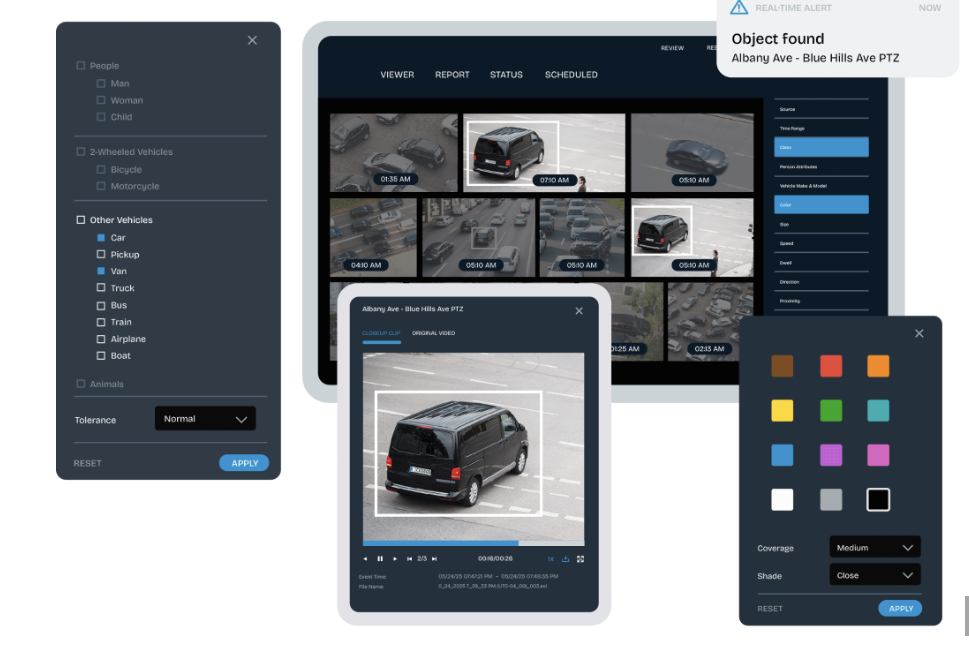
\includegraphics[width=0.6\textwidth]{briefcam.png}
    \caption{The search and filtering interface of BriefCam~\cite{milestone2026briefcam}}
    \label{fig:briefcam}
\end{figure}

\paragraph{Relation to the project.} BriefCam searches by attributes and by a sample object selected in recorded video, not an uploaded image as in this project; its documentation does not mention natural-language search.

\subsection{Avigilon Appearance Search}
\label{sec:2.1.2}

Avigilon Appearance Search is the deep-learning video search technology of Avigilon, part of Motorola Solutions, used to find a person or vehicle across hours of video from many cameras~\cite{motorola2021appearance}. A search can start by choosing appearance features from a predefined list such as clothing colour, gender and age group; by uploading an image; or by selecting an object in the video as a sample~\cite{motorola2021appearance}. The results help trace the route of the subject and can be bookmarked and exported as an evidence package describing the event. Figure~\ref{fig:avigilon} shows the interface with a person marked. The technology is built into the Avigilon Control Center video management software and runs on the vendor's cameras and recorders, or on the Avigilon AI Appliance for third-party ONVIF cameras.

\begin{figure}[H]
    \centering
    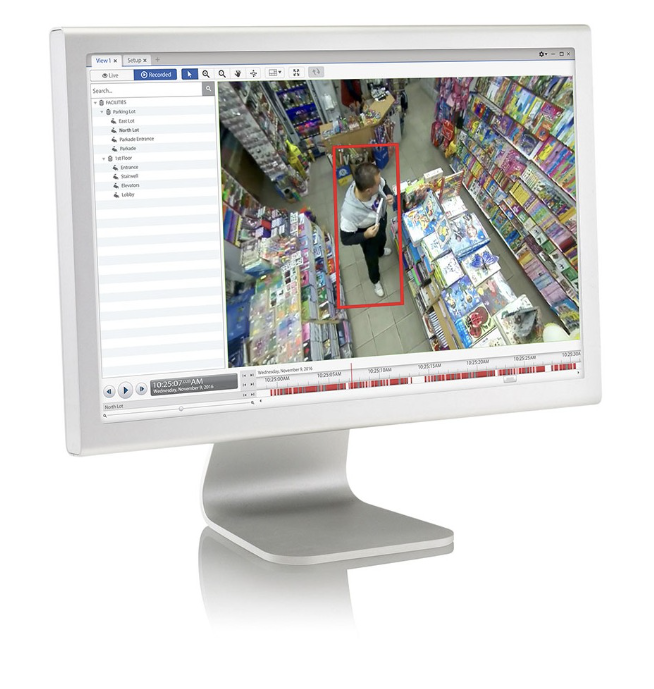
\includegraphics[width=0.45\textwidth]{avigilon.png}
    \caption{Avigilon Control Center with a marked subject~\cite{avigilon2026appearance}}
    \label{fig:avigilon}
\end{figure}

\paragraph{Relation to the project.} Avigilon supports two of the project's forms of description, attributes and a reference image, and compiles results into evidence like the project's case files; free-text search is not mentioned, and it is tied to the vendor's software and devices.

\subsection{Verkada AI-Powered Search}
\label{sec:2.1.3}

Verkada AI-Powered Search, introduced in 2024 on the Command cloud security platform, lets users search for people and vehicles in everyday language, for example ``person wearing helmet'', instead of choosing from a list of attributes~\cite{verkada2024aisearch}, and search with an uploaded image of a person, vehicle or object~\cite{verkada2024reverse}. According to the vendor's technical article~\cite{verkada2025scaling}, cameras produce crops of objects; in the cloud, the crops are encoded into vectors with the CLIP model, which maps images and text into one representation space, and stored in a vector database; the query sentence is encoded the same way to find the nearest crops. Figure~\ref{fig:verkada} shows the results of a natural-language query. The system works best with Verkada cameras; third-party cameras connect through a Command Connector device with higher latency~\cite{verkada2024connector}.

\begin{figure}[H]
    \centering
    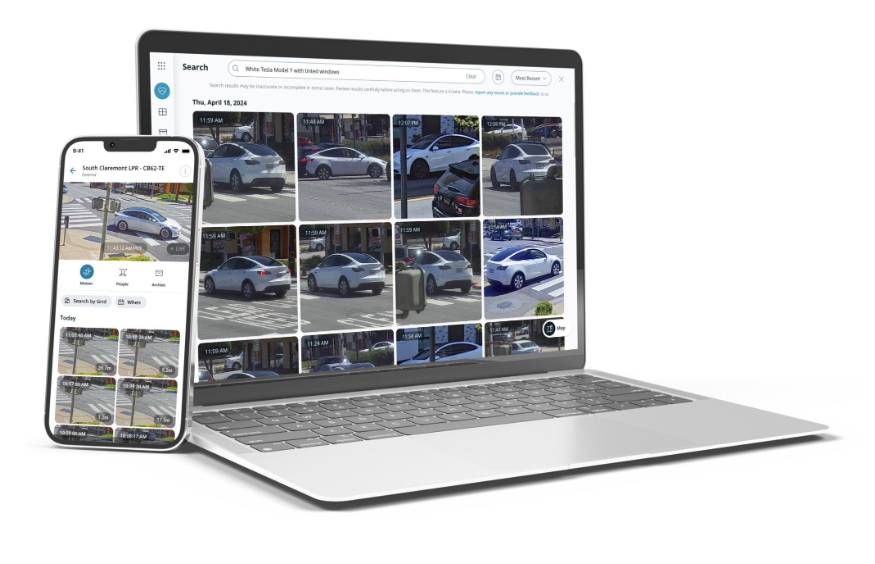
\includegraphics[width=0.52\textwidth]{verkada.png}
    \caption{Results of a natural-language query on the Verkada Command platform~\cite{verkada2024aisearch}}
    \label{fig:verkada}
\end{figure}

\paragraph{Relation to the project.} Verkada is technically closest: both search by description and by image through a shared representation space and a vector database. Verkada, however, runs on the vendor's cloud, while the project runs on premises on a commodity computer.

% !TEX root = ../../main.tex
% C2.2 - Comparison (translated). Only verified information from 2.1; "not mentioned" where the vendor says nothing.
\section{Comparison and Discussion}
\label{sec:2.2}

Table~\ref{tab:related-comparison} compares the three systems with the project, based on the vendors' documentation; anything not stated is marked ``not mentioned''.

\begin{longtable}{|>{\raggedright\arraybackslash}p{2.2cm}|>{\raggedright\arraybackslash}p{2.85cm}|>{\raggedright\arraybackslash}p{2.85cm}|>{\raggedright\arraybackslash}p{2.85cm}|>{\raggedright\arraybackslash}p{2.85cm}|}
\caption{Comparison of systems for searching people in video}\label{tab:related-comparison}\\
\hline
\textbf{Criterion} & \textbf{BriefCam} & \textbf{Avigilon Appearance Search} & \textbf{Verkada AI-Powered Search} & \textbf{The project's system} \\
\hline
\endfirsthead
\multicolumn{5}{l}{\textit{(continued from Table~\ref{tab:related-comparison})}}\\
\hline
\textbf{Criterion} & \textbf{BriefCam} & \textbf{Avigilon Appearance Search} & \textbf{Verkada AI-Powered Search} & \textbf{The project's system} \\
\hline
\endhead
Search by attributes & Yes: object type, colour, size, speed, direction & Yes: clothing colour, gender, age group; vehicle type and colour & Yes, predefined attribute filters, extended by natural-language search & Yes: gender, type and colour of upper and lower garments, carried items; converted into a description sentence \\
\hline
Search by image or appearance sample & Yes: select a sample object in the video to find similar appearances & Yes: upload an image or select a sample in the video & Yes: upload an image of a person, vehicle or object & Yes: upload a cropped image containing one person \\
\hline
Free-text search & Not mentioned & Not mentioned & Yes & Yes (English only) \\
\hline
Published matching mechanism & Metadata search and appearance similarity & Deep learning on appearance features, combined with facial features & Crops and query sentences encoded into one representation space (CLIP), searched in a vector database & Images, sentences and attributes encoded into one representation space, searched in a vector database \\
\hline
Other functions & Video Synopsis, face recognition, licence plates, real-time alerts, statistics and heat maps & Bookmarking and exporting results as evidence, multi-site search & Alerts created from a query, centralised cloud management & Case files, access control by role and surveillance area, overview dashboard of case files \\
\hline
Deployment model & On premises or on a cloud server & On premises, integrated with the vendor's video management software & The vendor's cloud platform & On premises on one personal computer \\
\hline
Hardware and device requirements & Processing server must have an NVIDIA graphics card & The vendor's cameras and recorders, or an AI Appliance for third-party ONVIF cameras & The vendor's cameras, or a Command Connector for third-party cameras & No discrete graphics card; receives streams from any RTSP camera \\
\hline
Distribution & Commercial software & Commercial software and devices & Commercial service platform & Self-developed application using published models \\
\hline
\end{longtable}

The comparison leads to the following observations:
\begin{itemize}
    \item \textbf{Supporting several forms of description has become the norm.} All three search by attributes and by an image or sample, but only Verkada offers free-text search (since 2024), encoding images and sentences into one space searched in a vector database, so one mechanism serves both forms.
    \item \textbf{Search usually comes with tools for compiling results}, such as Avigilon's bookmarks and evidence export, since investigators need to store and share results.
    \item \textbf{Commercial systems are tied to the vendor's infrastructure}: BriefCam needs a graphics card, Avigilon the vendor's software and devices, Verkada the vendor's cloud. Cost and lock-in are barriers for small organisations or those that must keep data on premises, and the products bundle many functions beyond search.
\end{itemize}

% !TEX root = ../../main.tex
% C2.3 - Development directions (translated).
\section{Development Directions}
\label{sec:2.3}

From these observations, the project sets the following directions:
\begin{enumerate}
    \item \textbf{Support all three forms of description in one search mechanism}: a reference image, an English description and predefined attributes, all mapped into one representation space as in Verkada; attributes become a structured sentence, so no per-attribute model is needed.
    \item \textbf{Organise results by appearance}, one appearance of a person on one camera, ranked by relevance and shown with the original frame for the user to judge (Section~\ref{sec:1.2}).
    \item \textbf{Manage results as case files}, like Avigilon's evidence compilation, so they can be reviewed without searching again.
    \item \textbf{Control access by role and surveillance area}, separating administration, searching and following results, with searchers limited to their area (Section~\ref{sec:1.1}).
    \item \textbf{Deploy on premises, independent of hardware vendors}: a web application that receives RTSP streams and processes and stores all data on a computer without a discrete graphics card.
\end{enumerate}


% !TEX root = ../../main.tex
% Chapter 3 (Part I) - translated from the Vietnamese edition.
\chapter{Theoretical Background}
\label{chapter:lythuyet}

\textit{This chapter presents the background of the application: person search and cross-modal retrieval, techniques for detecting and tracking people, frame sampling, joint image-text representation learning, vector search and the protocol used to stream camera video.}

% !TEX root = ../../main.tex
% C3.1 - Person search and cross-modal retrieval (translated).
\section{Person Search and Cross-Modal Retrieval}
\label{sec:3.1}

\subsection{Problem Statement}
\label{sec:3.1.1}

Given a set of person images extracted from the video of many cameras, called the \emph{gallery} $\mathcal{G} = \{g_1, g_2, \ldots, g_n\}$, and a \emph{query} $q$ describing the person being sought, the system must rank the elements of $\mathcal{G}$ by how well they match $q$ and return the $k$ best matches. The common approach is to learn a representation function that maps the query and every element into a vector space, then measure relevance with a similarity function $s(q, g_i)$; search then becomes finding the nearest vectors.

In surveillance data, the people to be indexed are not available as tightly cropped images as in benchmark datasets; they appear in full frames together with many other people and objects, so the complete problem also includes a person detection step. Xiao et al.\ learn detection and identification jointly in one model~\cite{xiao2017personsearch}; another approach uses a separate detector and a separate identification model~\cite{zheng2017reidwild}. The project follows the second approach so that each component can be replaced independently.

\subsection{Three Forms of Query}
\label{sec:3.1.2}
\label{sec:3.1.3}
\label{sec:3.1.4}

\paragraph{Search by image.} When the query is an image containing the person, the problem corresponds to \emph{person re-identification} (ReID): finding the images of the same person in data collected from several cameras or at several times~\cite{ye2022reidsurvey}. The main challenges are changes in viewpoint, lighting and pose, occlusion and low resolution: the same person can look very different between two cameras, while two people dressed alike can look very similar.

\paragraph{Search by text.} When the user only has a verbal description, for example ``a man wearing a black jacket and blue jeans, carrying a backpack'', the problem is text-based person search (TBPS), proposed by Li et al.\ together with the CUHK-PEDES dataset of person images with English descriptions~\cite{li2017cuhkpedes}. It is a cross-modal problem: the model must bring text and images into one representation space, while descriptions are often vague and the differences between people often lie in small details.

\paragraph{Search by attributes.} The user chooses appearance attributes from a predefined list such as gender, garment type and colour, and carried items. There are two ways to implement it: use a pedestrian attribute recognition model~\cite{wang2022parsurvey} and filter by label, which needs labelled data for every attribute; or combine the attributes into a description sentence from a fixed template and handle it as a text query. The project uses the second way so that it shares the model of text search; the trade-off is that attributes only affect the ranking and are not hard filters. Negative options such as ``no backpack'' are not supported, because CLIP-style vision-language models have considerable difficulty with negation, in many cases performing at chance level~\cite{alhamoud2025negation}.

Appearance search differs from face recognition: it does not rely on biometric features, which need a clearly visible face, but on clothing, colours and carried items, which are easy to observe from cameras mounted high and far away but can change and be shared by many people. The results are therefore suggestions for the user to assess, not conclusions about identity.

\subsection{Approach of the Project}
\label{sec:3.1.6}

Table~\ref{tab:query-modes} summarises the three forms of query and how the project handles them.

\begin{table}[H]
\centering
\caption{The three forms of describing the person and how the project handles them}
\label{tab:query-modes}
\begin{tabularx}{\textwidth}{|>{\raggedright\arraybackslash}p{2.6cm}|L|L|L|}
\hline
\textbf{Form} & \textbf{Input} & \textbf{Strengths and challenges} & \textbf{Handling in the project} \\
\hline
Reference image (ReID) & A cropped image containing one person & Rich visual information; sensitive to viewpoint, lighting and occlusion & Encoded with the image encoder \\
\hline
Text description (TBPS) & An English sentence & No image needed; descriptions may be vague or incomplete & Encoded with the text encoder \\
\hline
Attributes & Gender, type and colour of the upper and lower garments, carried items & Easy to enter and unambiguous; only expresses the available attributes & Turned into a structured English sentence, then handled as a text description \\
\hline
\end{tabularx}
\end{table}

\begin{itemize}
    \item \textbf{One shared representation space.} The RaSa model~\cite{bai2023rasa} encodes both images and text into one vector space, so person images from video, query images, description sentences and sentences generated from attributes can all be compared directly (Section~\ref{sec:3.5}).
    \item \textbf{The result unit is an appearance.} People are detected and tracked across frames (Sections~\ref{sec:3.2} and~\ref{sec:3.3}); each continuous appearance of a person on one camera (a track) is represented by one representative frame and one vector, which reduces the number of elements to match and avoids duplicate results.
    \item \textbf{Two separate stages.} The indexing stage runs in the background, processes camera streams and stores features; the query stage only encodes the user's description and finds the nearest vectors (Section~\ref{sec:3.6}), without processing images again.
    \item \textbf{A human makes the final decision.} The system only ranks; users assess each result on the original image before saving it to a case file.
\end{itemize}

% !TEX root = ../../main.tex
% C3.2 - Person detection (translated). Matches config/ultralytics_yolo_detector.json (conf 0.1, iou 0.7, max 300).
\section{Person Detection}
\label{sec:3.2}

\subsection{Object Detection}
\label{sec:3.2.1}

Object detection locates the objects in an image and determines their class. For each object, the model returns a rectangular \emph{bounding box}, usually given by the coordinates of two corners $(x_1, y_1, x_2, y_2)$, the \emph{class} of the object and a \emph{confidence score}. Two boxes are compared with the Intersection over Union (IoU):
\begin{equation}
    \mathrm{IoU}(A, B) = \frac{|A \cap B|}{|A \cup B|},
    \label{eq:iou}
\end{equation}
which ranges from 0 when the boxes do not overlap to 1 when they coincide. IoU is used to remove duplicate predictions and to link detections across frames in tracking (Section~\ref{sec:3.3}).

\subsection{Two-Stage and One-Stage Detectors}
\label{sec:3.2.2}

A \emph{two-stage} model such as Faster R-CNN~\cite{ren2017fasterrcnn} first uses a region proposal network to generate regions likely to contain objects, then classifies each region and refines its box; this is accurate but costly because many proposals must be processed. A \emph{one-stage} model such as YOLO (You Only Look Once)~\cite{redmon2016yolo} treats detection as a single regression problem, predicting the boxes and classes of all objects in one pass over the image, which is considerably faster and suits processing many video frames.

\subsection{The YOLO Family}
\label{sec:3.2.3}

Modern YOLO models have three parts: a feature extractor (backbone) at several levels of detail, a feature aggregator (neck) at several scales so that both large objects close to the camera and small distant ones can be detected, and a prediction head for boxes, classes and confidence. YOLO11 was released by Ultralytics in 2024 in five sizes (n, s, m, l, x) that trade speed for accuracy~\cite{ultralytics2024yolo11docs}. The models are pre-trained on COCO~\cite{lin2014coco}, which has 80 common object classes including \emph{person}, so they can detect people directly without further training.

\subsection{Post-Processing: Thresholding and Duplicate Removal}
\label{sec:3.2.4}

The raw output has many low-confidence and overlapping boxes. Boxes below a confidence threshold are discarded, and Non-Maximum Suppression (NMS) keeps the most confident box and removes same-class boxes overlapping it beyond an IoU threshold. A lower confidence threshold misses fewer people but adds false detections; a lower IoU threshold removes overlaps more aggressively but may merge people standing close together.

\subsection{Role of Detection in the System}
\label{sec:3.2.5}

The detector is applied to the sampled frames (Section~\ref{sec:3.4}) and keeps only the \emph{person} class, with a confidence threshold of 0.1, an NMS IoU threshold of 0.7 and at most 300 detections per frame. The low threshold is deliberate: ByteTrack needs low-confidence detections, often partially occluded people, to keep tracks alive (Section~\ref{sec:3.3}); they never start tracks, and a track needs two observations to be confirmed, so most transient false detections are removed by tracking. The reasons for choosing YOLO11n are given in Section~\ref{sec:6.1.4}.

% !TEX root = ../../main.tex
% C3.3 - Multi-object tracking (translated). Matches config/bytetrack_tracker.json and botsort_tracker.json.
\section{Multi-Object Tracking}
\label{sec:3.3}

\subsection{Problem and Basic Components}
\label{sec:3.3.1}
\label{sec:3.3.2}

A detector treats frames independently and cannot tell whether a person is the one seen before. Multi-Object Tracking (MOT) gives each object an identifier kept across frames; the sequence of its boxes is a \emph{track}, which in the project becomes an \emph{appearance}, the unit of search results (Section~\ref{sec:3.1.6}).

The common approach is \emph{tracking-by-detection}, founded on the SORT algorithm~\cite{bewley2016sort}, which has three components. First, each track has a Kalman filter~\cite{kalman1960} that predicts the position and size of its box in the current frame under a near-constant-velocity assumption, then corrects the prediction with the actual detection. Second, the match between a track and a detection is measured by the IoU (Equation~\ref{eq:iou}) between the predicted box and the detected box. Third, assigning each detection to at most one track at minimum total cost is solved with the Hungarian algorithm~\cite{kuhn1955hungarian}; an unmatched detection may start a new track, and an unmatched track is considered lost.

\subsection{ByteTrack}
\label{sec:3.3.3}

Earlier methods discarded low-confidence detections, so partially occluded people often broke their tracks. ByteTrack~\cite{zhang2022bytetrack} associates twice: high-confidence detections are matched with all tracks first, then the remaining tracks with low-confidence detections, so occluded people keep their tracks; unmatched low-confidence detections are dropped as mostly background. Only high-confidence detections start tracks, and a lost track is kept briefly so it can resume.

\subsection{BoT-SORT}
\label{sec:3.3.4}

BoT-SORT~\cite{aharon2022botsort} extends ByteTrack by adjusting the Kalman filter state, compensating camera motion and adding appearance re-identification (ReID) features to the association step. In the project, BoT-SORT is an alternative tracker with the same thresholds as ByteTrack; camera motion compensation and ReID are disabled because the cameras are static and to keep the cost low on a CPU-only machine.

\subsection{Track Life Cycle in the System}
\label{sec:3.3.5}

The tracker receives the detections of the sampled frames, separately for each camera, with the following rules:
\begin{itemize}
    \item \textbf{Confidence thresholds:} detections of 0.25 or more are high and may start a new track; detections from 0.1 to below 0.25 are only used in the second association step.
    \item \textbf{Confirmation:} a track is confirmed only after at least two observations; an unconfirmed track produces no result.
    \item \textbf{Termination:} a track ends after more than three lost processed frames or two seconds without observation, or when the stream ends. Both video files and RTSP streams use the timestamps recorded in the stream itself (Section~\ref{sec:3.7.4}), so the rule measures the time that passed in front of the camera and does not depend on how fast the machine processes.
    \item \textbf{Identifier scope:} one camera and one processing session only; the system does not link the tracks of the same person across cameras.
\end{itemize}

% !TEX root = ../../main.tex
% C3.4 - Frame sampling (translated). Matches workers/sampling.py (i mod N = 0; baseline N=10, throughput N=20 default).
\section{Frame Sampling}
\label{sec:3.4}
\label{sec:3.4.3}

The project's videos have about 60 frames per second, so consecutive frames are about 17 milliseconds apart and almost identical, and running the models on every frame is costly for little new information. Frames are sampled uniformly by index: frame $i$ is selected with sampling interval $N$ if and only if
\begin{equation}
    i \bmod N = 0,
    \label{eq:sampling}
\end{equation}
and it keeps its original index and timestamp, so that the time at which a person appears follows the camera's own timeline. With a source of $f$ frames per second, two processed frames are $N/f$ seconds apart: about 0.17 seconds with $N = 10$ and 0.33 seconds with $N = 20$.

The interval is a trade-off. Sampling precedes the detector, so model runs drop about $N$ times, but every frame must still be decoded, since most H.264 frames depend on earlier ones (Section~\ref{sec:3.7.1}). A larger $N$ misses brief appearances more easily, since a track needs two observations, and lets people move further between observations, making IoU association harder. The system provides two presets: \emph{baseline} with $N = 10$, which favours track quality, and \emph{throughput} with $N = 20$, which favours speed and was chosen as the default based on measurements on the target machine (Section~\ref{sec:8.5}). Each job records the value of $N$ it used so that results can be compared and reproduced.

% !TEX root = ../../main.tex
% C3.5 - Joint image-text representation learning (translated). RaSa (bai2023rasa), CLIP, ALBEF.
\section{Joint Image-Text Representation Learning}
\label{sec:3.5}

\subsection{Joint Embedding Space and Contrastive Learning}
\label{sec:3.5.1}
\label{sec:3.5.2}

To compare a description with a person image, the system uses two encoders: an image encoder turns an image into a feature vector, and a text encoder turns a sentence into a vector of the same dimension. The two encoders are trained so that the vector of an image and the vector of the sentence describing that image are close, while non-matching pairs are far apart; a space with this property is called a \emph{joint embedding space}. Closeness is measured with the cosine similarity
\begin{equation}
    s(\mathbf{u}, \mathbf{v}) = \frac{\mathbf{u}^\top \mathbf{v}}{\lVert \mathbf{u} \rVert \, \lVert \mathbf{v} \rVert},
    \label{eq:cosine}
\end{equation}
which becomes the inner product $\mathbf{u}^\top \mathbf{v}$ when the vectors are normalised to unit length (L2 normalisation). An important advantage is that the gallery images only need to be encoded once, at indexing time; at query time, the system only encodes the query and compares it with the stored vectors (Section~\ref{sec:3.1.6}).

The common training method is \emph{contrastive learning}: in each batch of $B$ image-text pairs, the correct sentence of an image is the positive sample, the other $B-1$ sentences are negatives, and the loss
\begin{equation}
    \mathcal{L}_i = -\log \frac{\exp\left(s(\mathbf{v}_i, \mathbf{t}_i)/\tau\right)}{\sum_{j=1}^{B} \exp\left(s(\mathbf{v}_i, \mathbf{t}_j)/\tau\right)}
    \label{eq:contrastive}
\end{equation}
pushes the similarity to the positive well above the negatives, with $\tau$ a temperature parameter; the text-to-image direction is computed the same way. CLIP~\cite{radford2021clip} applies this method to about 400 million image-text pairs from the Internet. ALBEF~\cite{li2021albef} first aligns the representations of the two modalities with contrastive learning, then fuses them in a multimodal encoder using cross-attention to match individual words with image regions in detail.

\subsection{The RaSa Model}
\label{sec:3.5.3}

General models such as CLIP and ALBEF struggle to separate small differences between people who look alike, for example the same jacket with trousers of a different colour. RaSa (Relation and Sensitivity Aware representation learning)~\cite{bai2023rasa} is built on ALBEF and designed specifically for text-based person search, with a 12-layer transformer image encoder, a 6-layer text encoder and a 6-layer multimodal encoder. Its three key points are:
\begin{itemize}
    \item \textbf{Intra- and inter-modal contrastive learning.} Besides pairing images with sentences, images of the same person are also pulled together. This makes the vectors of two images of one person close, which is the basis for using the same vector space for image queries in the project.
    \item \textbf{Relation-aware learning.} Each description is written for \emph{one} specific image and may not be fully true of the other images of that person; RaSa separates these two kinds of positive pairs so as not to learn details that are not true.
    \item \textbf{Sensitivity-aware learning.} The model is trained to notice when an important word is replaced, such as ``red shirt'' becoming ``blue shirt'', which changes the meaning of the sentence.
\end{itemize}
At query time, RaSa can re-rank the top 128 results with the multimodal encoder to improve accuracy, but this is far more costly than comparing vectors alone. On the CUHK-PEDES test set, RaSa reaches a Rank-1 of 76.51\% and an mAP of 69.38\%~\cite{bai2023rasa}.

\subsection{Use of RaSa in the System}
\label{sec:3.5.4}

The system uses RaSa weights pre-trained on CUHK-PEDES, without retraining. The image encoder encodes the person image cropped from the representative frame at indexing time and the query image when searching by image, with input images resized to $384 \times 384$ pixels; the text encoder encodes description sentences and sentences generated from attributes. Vectors have 256 dimensions and are L2-normalised, so all three kinds of query are compared with the same set of vectors by inner product, and each track needs only one vector. Re-ranking is not enabled, because it only applies to text queries, is costly on a CPU-only machine, and no measurement yet shows that it improves results on the project's data.

Two points should be noted. First, RaSa was designed and evaluated for text-based search; using its image encoder for image-to-image queries is the project's choice based on its intra-modal contrastive learning, not a published result. Second, CUHK-PEDES was built from the images of five existing person re-identification datasets~\cite{li2017cuhkpedes}, each image being a tightly cropped person with a sentence written for that image; the person images in the project are cropped automatically from full frames of a crowded area, with a different context and viewpoint, and are often partially occluded by the people around them. This domain gap directly affects the quality of text and attribute queries (Section~\ref{sec:8.4}).

% !TEX root = ../../main.tex
% C3.6 - Vector search (translated). HNSW (malkov2020hnsw), Milvus (wang2021milvus) and its docs.
% Matches storage/milvus/vectors.py (HNSW, IP, M=16, efConstruction=128, ef=64) and services/track_search.py.
\section{Vector Search}
\label{sec:3.6}

\subsection{Nearest Neighbour Search and the HNSW Index}
\label{sec:3.6.1}
\label{sec:3.6.2}

With one vector per appearance and a query vector $\mathbf{q}$, search becomes \emph{$k$-nearest-neighbour}: find the $k$ of $n$ stored vectors with the largest inner product with $\mathbf{q}$. Exhaustive search is exact but grows linearly with $n$; \emph{Approximate Nearest Neighbor} (ANN) search uses a prebuilt index to examine only part of the data, trading a few missed neighbours for speed.

HNSW (Hierarchical Navigable Small World)~\cite{malkov2020hnsw} is a graph-based ANN method: each vector links to some nearby vectors, and search keeps moving to a neighbour closer to the query. Sparse upper layers reach the right region quickly and the bottom layer, holding every vector, searches it precisely, so cost grows logarithmically with the data~\cite{malkov2020hnsw}. The index has three main parameters~\cite{milvus2026hnsw}: the maximum number of edges per node $M$ and the number of candidates during construction \textit{ef\-Con\-struc\-tion}, which give a better graph when larger but cost more memory and construction time; and the number of candidates during search $\mathit{ef}$, which is more accurate but slower when larger and should not be smaller than the number of results requested.

\subsection{Vector Search with Filters}
\label{sec:3.6.3}

Surveillance queries carry conditions such as the user's area or a time range. \textbf{Post-filtering} takes the $k$ nearest vectors overall and then drops those failing the condition, so it may return few or no results when the area is a small part of the data. \textbf{Pre-filtering} searches only among the vectors meeting the condition, so results fall short of $k$ only when the scope really holds little data. Milvus~\cite{wang2021milvus}, an open-source vector database, stores scalar fields next to the vectors and performs search with pre-filtering~\cite{milvus2026filtered}.

\subsection{Vector Search in the System}
\label{sec:3.6.4}

The system uses Milvus with an HNSW index, the inner-product metric, $M = 16$, \textit{ef\-Con\-struc\-tion}~$= 128$ and $\mathit{ef} = 64$. A search sends Milvus the query vector together with a filter made of the user's area, the permitted cameras, the time range if any and the ready status, and receives at most $k$ results with $k \in \{4, 8, 12, 16\}$. The similarity, computed at query time, is shown as the relevance score. Each result is checked against PostgreSQL for its details and scope; invalid results caused by temporarily unsynchronised stores are dropped, and if fewer than $k$ remain, the search is repeated with twice the number, up to three rounds; $\mathit{ef}$ is raised to the number requested when the re-ranking stage of Section~\ref{sec:5.2.3} asks for a pool larger than 64, up to 128. Exhaustive search would still suffice for the 1,523-track demonstration data (Section~\ref{sec:7.2}); HNSW keeps response times as data accumulates.

% !TEX root = ../../main.tex
% C3.7 - RTSP and camera simulation (translated). RFC 2326/7826/3550/6184, H.264, FFmpeg, MediaMTX.
% Matches scripts/rtsp.ps1 and workers/sources/rtsp.py (PyAV, TCP, 8 s timeouts, 3 reconnects 0.25-2 s, worker-clock timestamps).
\section{RTSP and Camera Stream Simulation}
\label{sec:3.7}

\subsection{H.264 Compressed Video}
\label{sec:3.7.1}

IP cameras compress video, since an uncompressed 1920$\times$1080 frame takes about 6~MB, or about 370~MB per second at 60 frames per second. H.264~\cite{wiegand2003h264} is the common standard and the project's format. An \emph{I-frame} only uses prediction within the frame itself, so it can be decoded independently; \emph{P-frames} and \emph{B-frames} only store motion and differences relative to reference frames, so they can only be decoded once their references are available. Decoding must therefore be done on every frame even though the system only analyses some of them (Section~\ref{sec:3.4}), and a decoder that joins a stream midway must wait for the next I-frame.

\subsection{RTSP and RTP}
\label{sec:3.7.2}

RTSP (Real Time Streaming Protocol)~\cite{rfc2326} is a \emph{control} protocol: the receiver identifies a stream by an address of the form \texttt{rtsp://<host>:<port>/<path>} and exchanges the \texttt{DESCRIBE}, \texttt{SETUP}, \texttt{PLAY} and \texttt{TEARDOWN} commands to obtain the description, set up, start and end the session. The data is carried by RTP (Real-time Transport Protocol)~\cite{rfc3550}: compressed video is split into packets with sequence numbers and timestamps; for H.264 the timestamps use a 90~kHz clock~\cite{rfc6184}. RTP packets can be sent over UDP, with low latency but possible packet loss, or interleaved on the TCP connection of the RTSP session, without loss but possibly late under congestion. RTSP 2.0~\cite{rfc7826} removed the commands used to push a stream to a server, so the project's simulation tools use version 1.0.

\subsection{Simulating Cameras with a Streaming Server}
\label{sec:3.7.3}

To test with the real protocol of IP cameras, each video is replayed as an RTSP stream acting as one camera. The MediaMTX streaming server~\cite{mediamtx2026} accepts streams pushed in and serves streams out over RTSP, each at its own path such as \texttt{/cam1}. The FFmpeg tool~\cite{ffmpeg2026docs} reads the file and pushes it to MediaMTX with three options: \texttt{-re} to send at the original frame rate, \texttt{-stream\_loop -1} to loop forever like a camera that never stops, and \texttt{-c copy} to copy the compressed data without re-encoding, so the stream carries exactly the H.264 data of the original file and costs almost no resources. Like a real camera, the stream uses the same protocol and format and does \emph{not wait} for a slow receiver; unlike one, its content repeats and it suffers almost no packet loss or disconnection.

\subsection{Receiving RTSP Streams in the System}
\label{sec:3.7.4}

The background worker reads streams with the PyAV library, which uses FFmpeg's decoding libraries, with RTP interleaved over TCP to avoid packet loss corrupting images. Connecting and waiting for data are both limited to 8 seconds; when a stream is interrupted, the system tries to reconnect up to three times with a waiting time growing from 0.25 to 2 seconds, then records the processing run as failed. Each frame is timestamped from the stream's own presentation timestamp, anchored to the machine clock at the first frame of each session, so that the time between two processed frames is the stream time between them even when the machine falls behind; a session that starts again after a reconnection or a restart of the source is anchored again, and only a frame without a usable timestamp falls back to the reception time (Section~\ref{sec:3.3.5}). Processing is much slower than the stream, so cameras share processing time as described in Section~\ref{sec:5.2.1}.


% !TEX root = ../../main.tex
% Chapter 4 (Part I) - translated from the Vietnamese edition.
% Role names in the English edition: Administrator (Admin), Operator, Viewer - as in the specifications and the code.
\chapter{System Analysis}
\label{chapter:phantich}

\textit{This chapter analyses the requirements of the system: actors, functional and non-functional requirements, the use case model and the permission matrix.}

% !TEX root = ../../main.tex
% C4.1 - Actors (translated). First place that names the roles: Administrator, Operator, Viewer; Case.
\section{Actors}
\label{sec:4.1}

The system has three actors, corresponding to three kinds of user account divided by responsibility: the \textbf{Administrator} (Admin), the \textbf{Operator} and the \textbf{Viewer}. All three share one login function; after authentication, the system determines the role of the account and only offers the functions and data suited to that role.

Before describing each actor, two business concepts used throughout the following chapters need to be defined:
\begin{itemize}
    \item \textbf{Surveillance area:} a geographic scope such as a building or a public space. Each camera belongs to exactly one area, set when the camera is added and not changed afterwards. The list of areas is declared at deployment; the current version has no interface for adding, editing or deleting areas.
    \item \textbf{Case:} a record created by an Operator to keep the search results related to an incident, with a title, notes and a status of \emph{Open} or \emph{Closed}. A case belongs to the Operator in charge of it but is not tied directly to a surveillance area: the area only limits the scope of search, while the rights over a case follow its owner. Since an Operator's area can change, a case may contain results from several areas.
\end{itemize}

\subsection{Administrator}
\label{sec:4.1.1}

The Administrator is responsible for the \emph{technical administration} of the system, keeping the camera system and the AI processing running so that the other actors can use them. The Administrator's responsibilities are:
\begin{itemize}
    \item \textbf{Managing accounts} of Operators and Viewers, including assigning a surveillance area to each Operator.
    \item \textbf{Managing cameras} and the connection to the RTSP stream of each camera.
    \item \textbf{Managing AI processing:} deciding which cameras are analysed, and choosing the person detector (Detector) and the tracking algorithm (Tracker) used by the whole system.
    \item \textbf{Monitoring operation:} following the status of cameras and AI processing, checking the AI components, and consulting the audit log.
\end{itemize}

Technical administration rights do \emph{not} imply business rights: by default, the Administrator may not search for people and does not see cases. The Administrator account is created at deployment; through the interface, the Administrator can only create and assign the Operator and Viewer roles.

\subsection{Operator}
\label{sec:4.1.2}

The Operator uses the main business function of the system directly: searching for people in the analysed camera data and saving the matching results into cases. The Operator's responsibilities are:
\begin{itemize}
    \item \textbf{Searching for people} by image, English description or appearance attributes.
    \item \textbf{Assessing results:} viewing each result in the context of its frame and deciding which results really show the person being sought.
    \item \textbf{Managing cases:} saving matching results into cases and following each case until it is closed.
\end{itemize}

The Operator's scope is limited by two principles. First, the \emph{search scope} is set by the surveillance area attached to the account: the system only searches the operational cameras of that area, and rejects any request containing a camera or area outside the Operator's rights. Second, the \emph{case scope} is set by ownership: each case has exactly one Operator in charge, the one who created it; an Operator only acts on the cases he or she owns and cannot transfer ownership to someone else. The two scopes are independent: when moved to another area, an Operator still sees and manages his or her old cases, while new searches only run in the new area.

\subsection{Viewer}
\label{sec:4.1.3}

The Viewer is at the management level of the organisation, such as a head of department or a director, who needs to follow the results of the work but does not search or configure the system. The Viewer's responsibilities are:
\begin{itemize}
    \item \textbf{Viewing an overview} of the cases across the whole system.
    \item \textbf{Viewing cases:} every case and the results saved in it.
\end{itemize}

The Viewer only has read access and does not search for people. Unlike the Operator, the Viewer is not limited by area, because the Viewer's scope is the cases, which are not tied to areas.

\subsection{Principles of Role Separation}
\label{sec:4.1.4}

The division above follows two principles: \textbf{separating technical rights from business rights}, so that the people who configure the system do not automatically access search data and the people who use the data cannot interfere with the configuration; and \textbf{least privilege}, so that each actor only has the rights needed for its work. The rights of each role for each group of actions are summarised in the permission matrix of Section~\ref{sec:4.6}.

The camera streams and the background AI processing are not actors: a camera is a data source configured by the Administrator, and the analysis of camera data is performed automatically by the system when AI processing is enabled, not triggered directly by a user.

% !TEX root = ../../main.tex
% C4.2 - Functional requirements (translated). Codes: FR-C (common), FR-A (Administrator), FR-O (Operator),
% FR-V (Viewer), FR-S (automatic system functions).
\section{Functional Requirements}
\label{sec:4.2}

The functional requirements are grouped by the actors of Section~\ref{sec:4.1}, together with a group of common functions and a group of functions the system performs by itself. Each requirement has a code for cross-reference with the use case specifications (Section~\ref{sec:4.5}) and the test results (Chapter~\ref{chapter:kiemthu}).

\subsection{Common Functions}
\label{sec:4.2.1}

\begin{reqlist}
    \item[FR-C01] Users log in with a username and password and are taken to the interface of their role; locked or deactivated accounts are rejected.
    \item[FR-C02] Users can log out. A session expires 12 hours after it is issued or after 30 minutes of inactivity, and becomes invalid immediately when the account is locked or deactivated. While the user is active, the session is refreshed with a new session.
\end{reqlist}

\subsection{Administrator Functions}
\label{sec:4.2.2}

\paragraph{Account management.}
\begin{reqlist}
    \item[FR-A01] Create, update, lock, unlock, delete or deactivate accounts, assigning the Operator or Viewer role; usernames are unique.
    \item[FR-A02] Each Operator is assigned exactly one surveillance area, chosen from the predefined list.
\end{reqlist}

\paragraph{Camera management.}
\begin{reqlist}
    \item[FR-A03] Add and update cameras with a code, name, area, RTSP address and credentials; the camera code is unique, and the area cannot be changed after creation.
    \item[FR-A04] Check the RTSP connection when a camera is added, when its address changes and on request; if the connection fails, the camera is still saved with a warning so that it can be checked again later.
    \item[FR-A05] Retire a camera from operation or bring it back. The data of a retired camera is kept but cannot be searched or added to cases for the time being; results already saved in cases remain visible. A camera brought back into operation starts with AI processing disabled.
\end{reqlist}

\paragraph{AI processing management.}
\begin{reqlist}
    \item[FR-A06] Enable or disable AI processing for each camera; enabling is refused when the camera has lost its RTSP connection, has been retired or the models are not ready.
    \item[FR-A07] Upload a video file for a camera to be processed through the same pipeline as an RTSP stream; the function is used to prepare the demonstration data (Section~\ref{sec:1.3}) and for cameras without RTSP.
    \item[FR-A08] Choose the Detector and Tracker from a registered list, applied to the whole system; the configuration is only applied when the models are ready and the pair is compatible, otherwise the previous configuration is kept. The image and text encoders are fixed.
\end{reqlist}

\paragraph{Operation monitoring.}
\begin{reqlist}
    \item[FR-A09] Follow the RTSP connection and AI processing status of each camera, filter abnormal cameras and refresh the data.
    \item[FR-A10] Check the camera processing group, on a real frame from one camera, and the search group separately; results are shown per component, and a frame without people is reported as not yet verifiable rather than as an error.
    \item[FR-A11] View and filter the audit log by actor, event type and time. The log records logins, logouts, failed logins, administrative actions, case actions and important technical errors; it does not record searches.
\end{reqlist}

\subsection{Operator Functions}
\label{sec:4.2.3}

\paragraph{Searching for people.}
\begin{reqlist}
    \item[FR-O01] Search by image, provided by file selection, drag and drop, pasting, or dragging a result into the search box to search again for the same person.
    \item[FR-O02] Search by an English description; Vietnamese is not supported and nothing is translated automatically.
    \item[FR-O03] Search by attributes, namely gender, the type and colour of the upper and lower garments, and carried items, with no negative options; the attributes are combined into an English description and searched as in FR-O02.
    \item[FR-O04] The search scope is automatically limited to the account's area and can be narrowed further by operational camera and time range; requests containing cameras or areas outside the Operator's rights are rejected.
    \item[FR-O05] Choose 4, 8, 12 or 16 results; the system returns at most that many in decreasing order of relevance, without a score threshold that discards results.
\end{reqlist}

\paragraph{Viewing and assessing results.}
\begin{reqlist}
    \item[FR-O06] Each result is one appearance of a person on one camera, shown as the person image with surrounding context, rank, camera, area, time and relevance score.
    \item[FR-O07] Select a result to see the full frame with the person's bounding box and the details.
    \item[FR-O08] Sort results by relevance or time, and filter them again by camera or time.
\end{reqlist}

\paragraph{Case management.}
\begin{reqlist}
    \item[FR-O09] Create a new case from a result with a title and notes; the owner is always the logged-in account.
    \item[FR-O10] Add a result to an open case the Operator owns; each save creates a new entry, even for the same appearance.
    \item[FR-O11] Optionally close the case while saving; if that step fails, the result is still saved and the user is informed.
    \item[FR-O12] Edit the title and notes and remove results from an open case.
    \item[FR-O13] Close or reopen a case; the content of a closed case cannot be edited and results cannot be added or removed.
    \item[FR-O14] View the cases the Operator owns, including after a change of area; results are shown as in FR-O06 and FR-O07 but without the relevance score.
\end{reqlist}

\subsection{Viewer Functions}
\label{sec:4.2.4}

\begin{reqlist}
    \item[FR-V01] View a system-wide overview: the number of cases by status, the number of saved results and the list of recent cases; select a case to see its details.
    \item[FR-V02] View every case, filtered by status, creation time or the Operator in charge.
    \item[FR-V03] View the details of a case and its saved results in read-only mode.
    \item[FR-V04] View the details of a saved result and the full frame with its bounding box; the relevance score is not shown.
\end{reqlist}

\subsection{Automatic System Functions}
\label{sec:4.2.5}

\begin{reqlist}
    \item[FR-S01] Automatically analyse, in turn, the cameras that are operational, have AI processing enabled and have RTSP, so that every camera is analysed.
    \item[FR-S02] For each RTSP stream or video file: sample frames, detect people, track them into appearances, choose one representative frame and create a feature vector.
    \item[FR-S03] Store the representative frame, bounding box, vector and camera, area and time information of each appearance; an appearance can only be found once it is fully stored.
\end{reqlist}

% !TEX root = ../../main.tex
% C4.3 - Non-functional requirements (translated), NFR-01..23.
\section{Non-Functional Requirements}
\label{sec:4.3}

The quality requirements stem from three traits of the problem: camera data is sensitive, each appearance is stored in several parts that must stay consistent, and the system runs on a personal computer without a graphics card.

\subsection{Security and Access Control}
\label{sec:4.3.1}

\begin{reqlist}
    \item[NFR-01] \textbf{Server-side permission checks} for every request, images included, based on the login session rather than on data sent by the browser; hiding a function in the interface is not access control.
    \item[NFR-02] \textbf{Authentication:} passwords are only stored as one-way hashes, sessions follow FR-C02, and requests that change data are protected against cross-site request forgery (CSRF).
    \item[NFR-03] \textbf{Image protection:} frames are never publicly accessible; they only reach the browser through the server after a permission check.
    \item[NFR-04] \textbf{Camera connection protection:} RTSP credentials are encrypted and never shown again; the system only connects to the camera network ranges declared at deployment.
    \item[NFR-05] \textbf{Abuse limitation:} the number of calls to sensitive functions is limited, uploaded files are size-limited and format-checked, and error messages do not reveal internal information.
\end{reqlist}

\subsection{Data Integrity and Recoverability}
\label{sec:4.3.2}
\label{sec:4.3.3}

\begin{reqlist}
    \item[NFR-06] \textbf{Data consistency:} an appearance can only be found once its description, vector and frame are all stored; incomplete data must be completable or cleanable.
    \item[NFR-07] \textbf{No destruction of historical data:} retiring a camera, disabling AI processing, locking or deleting an account and removing a result from a case keep the original data; the cases of a locked or deleted account keep their owner and stay visible to Viewers.
    \item[NFR-08] \textbf{Case integrity:} results in a case keep a snapshot of the camera name, area and time; concurrent updates never silently overwrite each other.
    \item[NFR-09] \textbf{No mixing of vector spaces} from different encoder versions.
    \item[NFR-10] \textbf{Fault isolation:} a failing component only fails its own function, is reported by name and does not stop other cameras.
    \item[NFR-11] \textbf{Self-recovery:} the system reconnects automatically when an RTSP stream is interrupted.
    \item[NFR-12] \textbf{No misleading results:} unavailable search components produce an error, not an empty result; a missing image does not hide the other information.
    \item[NFR-13] \textbf{Safe retries:} multi-step operations leave a valid state when interrupted and can be retried without creating duplicate data.
\end{reqlist}

\subsection{Performance and Resources}
\label{sec:4.3.4}

\begin{reqlist}
    \item[NFR-14] \textbf{Runs on the target machine:} the whole system runs on an Intel Core i5-11300H laptop with 16~GB of memory and no discrete graphics card.
    \item[NFR-15] \textbf{Search independent of indexing:} analysis runs in the background and search only uses indexed data, so search stays usable during analysis.
    \item[NFR-16] \textbf{No real-time requirement:} streams need not be analysed in real time or concurrently; the sampling interval is chosen from presets.
\end{reqlist}

\subsection{Traceability, Usability and Maintainability}
\label{sec:4.3.5}
\label{sec:4.3.6}
\label{sec:4.3.7}

\begin{reqlist}
    \item[NFR-17] \textbf{The audit log} (FR-A11) cannot be modified, contains no passwords or credentials, and keeps the actor's information when the account is deleted.
    \item[NFR-18] \textbf{Reproducible provenance:} each appearance records the versions of the Detector, Tracker and encoder and the sampling interval used.
    \item[NFR-19] \textbf{Language:} the interface is in Vietnamese; only the query content is in English.
    \item[NFR-20] \textbf{Support for visual assessment:} person images are shown in context, the relevance score is for reference only, and the system neither concludes on identity nor shows the models' internal confidence.
    \item[NFR-21] \textbf{Several screen sizes:} usable on a computer and on a phone about 390 pixels wide.
    \item[NFR-22] \textbf{Replaceable models:} a new Detector or Tracker needs no change elsewhere; RTSP streams and video files share the pipeline after frame reading.
    \item[NFR-23] \textbf{Replaceable camera source:} standard RTSP lets real cameras replace the simulated streams without changing the pipeline.
\end{reqlist}

% !TEX root = ../../main.tex
% C4.4 - Use case diagram (translated). Figure H1 is the English version (figures/H1-use-case.png, generated from tools-en).
\section{Use Case Diagram}
\label{sec:4.4}

The functional requirements of Section~\ref{sec:4.2} are organised into 15 use cases. Figure~\ref{fig:usecase} shows all the use cases of the system with their relations and actors, and Table~\ref{tab:usecases} lists each use case with its actor and purpose.

\begin{figure}[H]
\centering
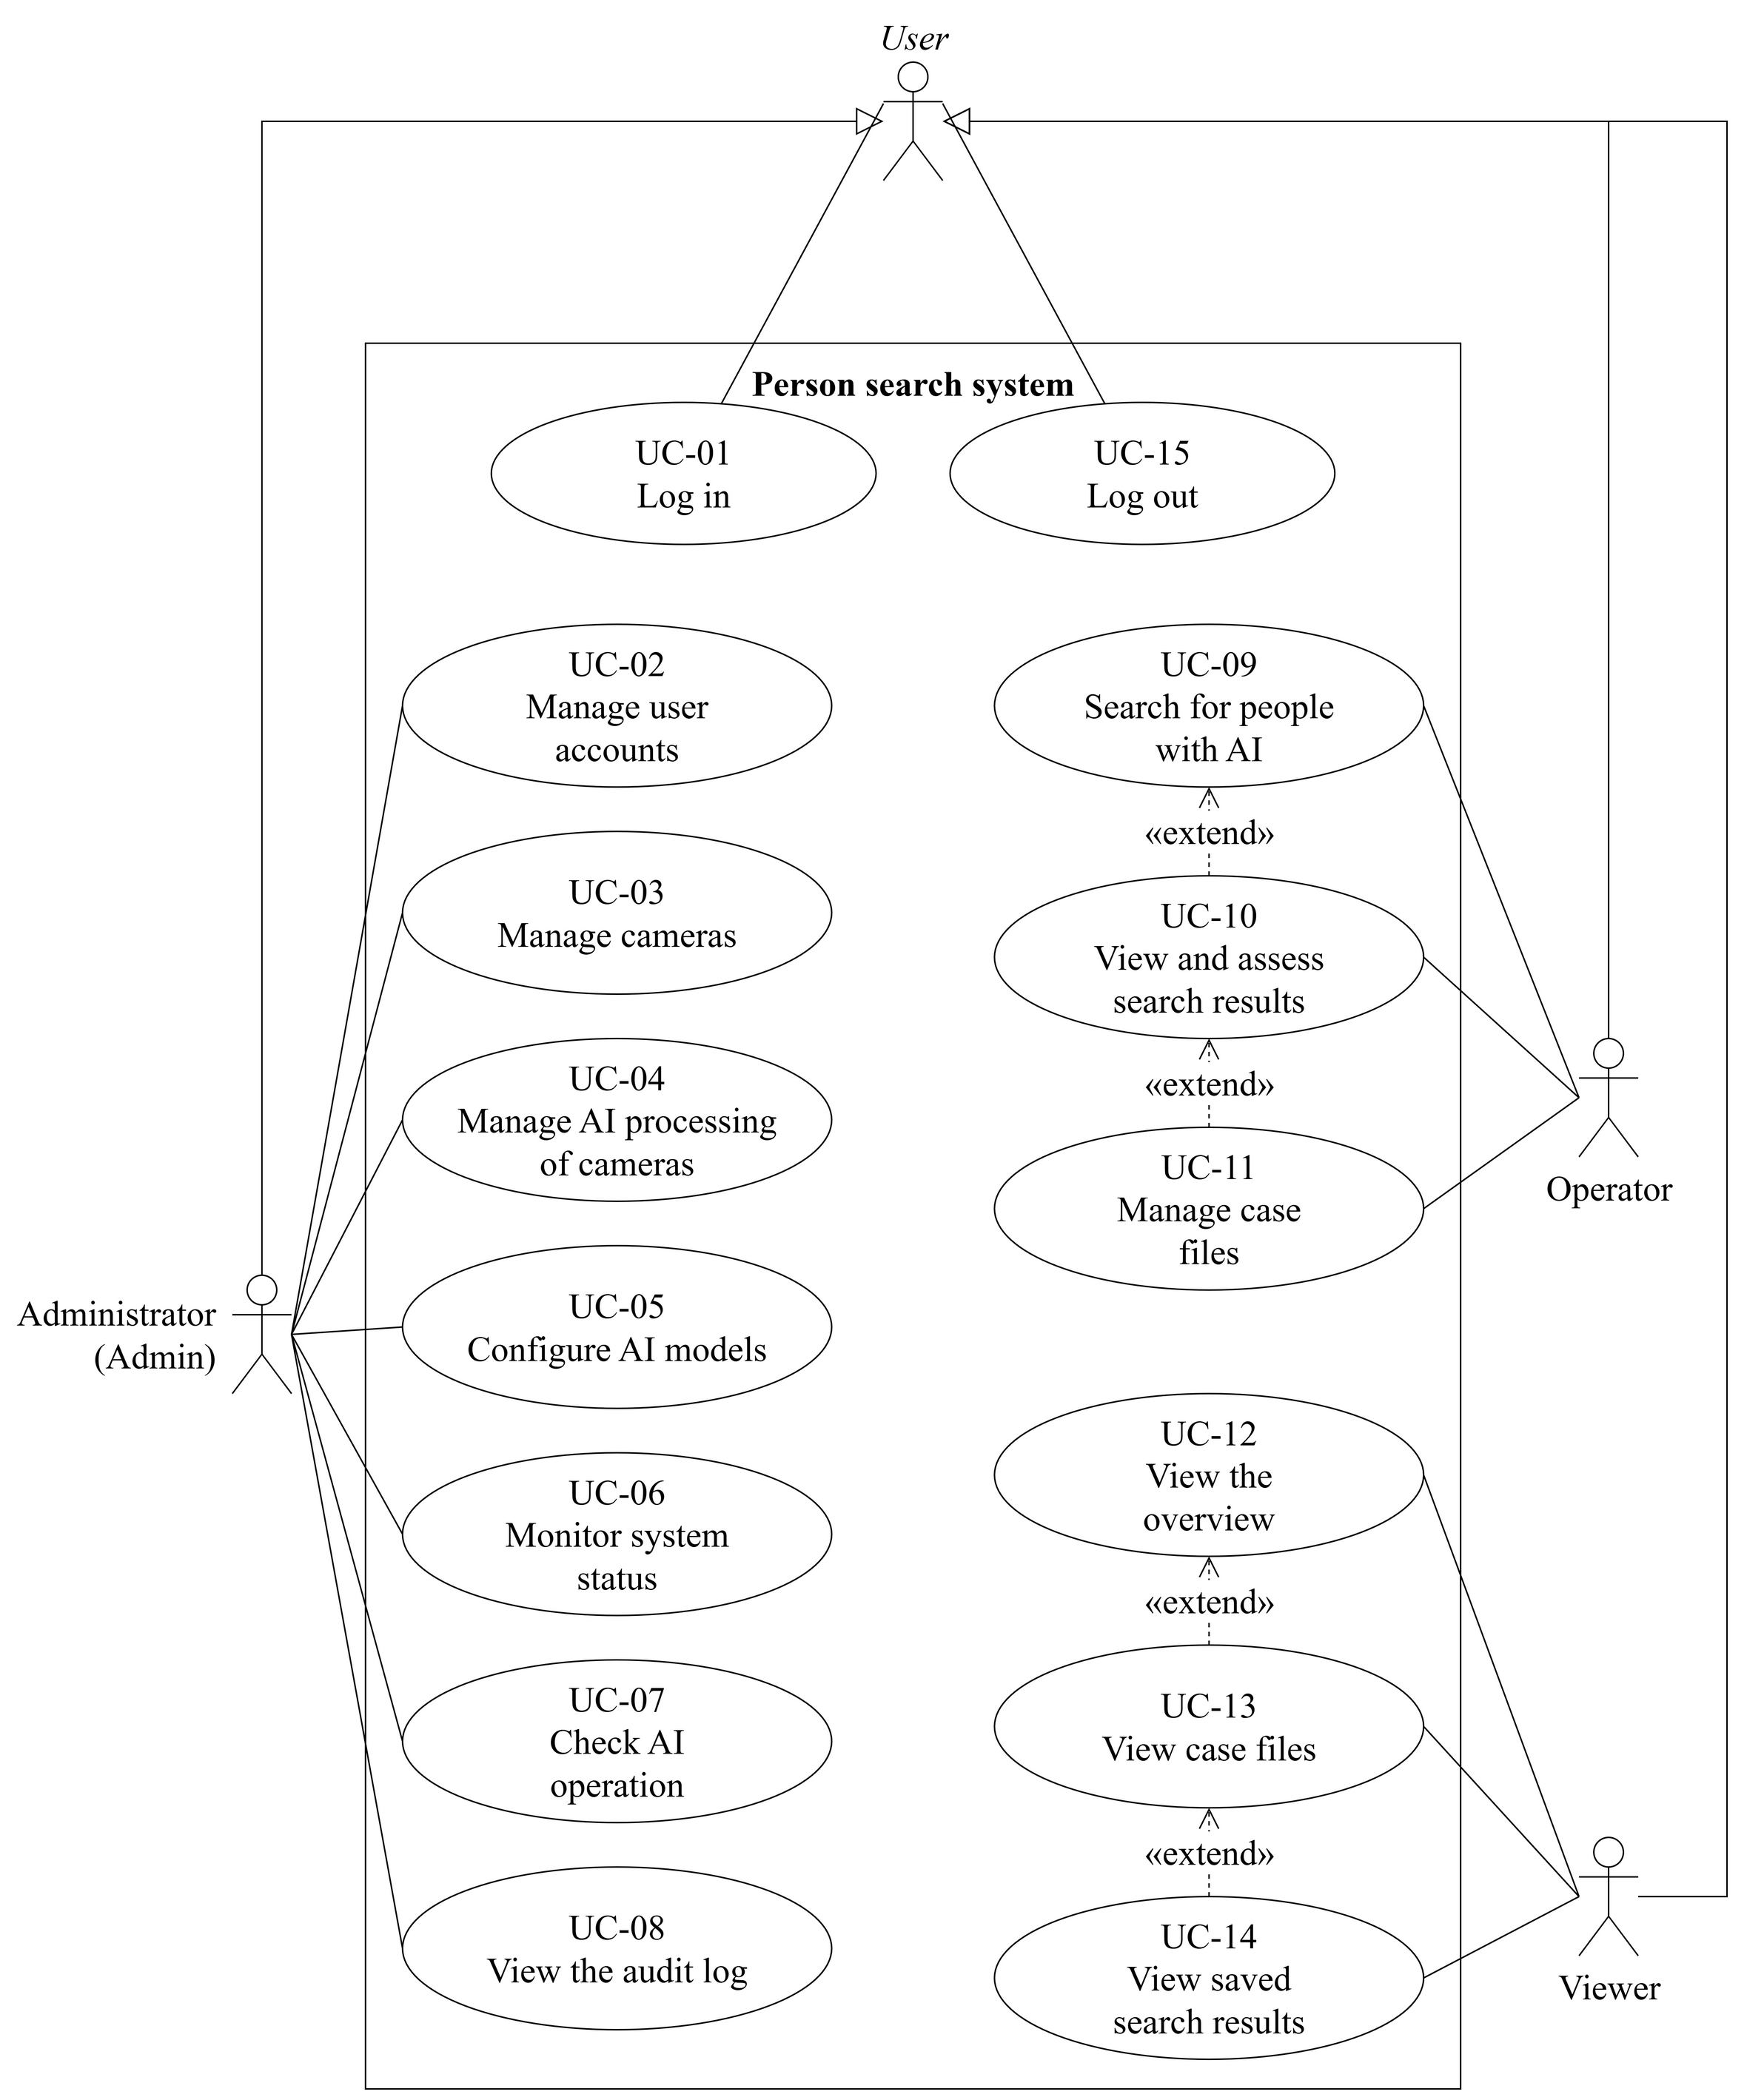
\includegraphics[width=\textwidth]{H1-use-case.png}
\caption{Use case diagram of the system}
\label{fig:usecase}
\end{figure}

The diagram is organised as follows:
\begin{itemize}
    \item \textbf{An abstract \emph{User} actor.} The three concrete actors share login (UC-01) and logout (UC-15), so the diagram links these two use cases to an abstract \emph{User} actor, which the three concrete actors generalise to.
    \item \textbf{Division by role.} The Administrator is linked to UC-02 to UC-08, the Operator to UC-09 to UC-11 and the Viewer to UC-12 to UC-14; no use case is shared among these actors.
    \item \textbf{Extend relations.} UC-10 extends UC-09 and UC-11 extends UC-10: after searching, the Operator can view the details of a result and then save it into a case. Likewise, UC-13 extends UC-12 and UC-14 extends UC-13. The extending use cases are still linked directly to their actor, because the actor can also start them independently, for example opening the list of cases without searching first.
    \item \textbf{Login is a precondition} of every other use case, not a step inside them, so the diagram draws no «include» relation to UC-01.
\end{itemize}

The automatic system functions (Section~\ref{sec:4.2.5}) have no use case of their own because no actor triggers them; they take place when the Administrator enables AI processing in UC-04.

\begin{table}[H]
\centering
\caption{List of use cases}
\label{tab:usecases}
\begin{tabularx}{\textwidth}{|>{\raggedright\arraybackslash}p{1.4cm}|>{\raggedright\arraybackslash}p{3.8cm}|>{\raggedright\arraybackslash}p{2.4cm}|L|}
\hline
\textbf{Code} & \textbf{Use case} & \textbf{Actor} & \textbf{Purpose} \\
\hline
UC-01 & Log in & All three actors & Authenticate and access the functions of the role \\
\hline
UC-02 & Manage user accounts & Administrator & Create, update, lock and delete accounts; assign roles and areas \\
\hline
UC-03 & Manage cameras & Administrator & Add and update cameras, check the RTSP connection, retire and restore them \\
\hline
UC-04 & Manage AI processing of cameras & Administrator & Enable or disable AI processing per camera; process fallback video files \\
\hline
UC-05 & Configure AI models & Administrator & Choose the Detector and Tracker used by the whole system \\
\hline
UC-06 & Monitor system status & Administrator & Follow the status of cameras, RTSP streams and AI processing \\
\hline
UC-07 & Check AI operation & Administrator & Check the camera processing group and the search group \\
\hline
UC-08 & View the audit log & Administrator & Consult the log of actions and technical events \\
\hline
UC-09 & Search for people with AI & Operator & Search by image, description or attributes within the assigned area \\
\hline
UC-10 & View and assess search results & Operator & View the details of each result, compare and assess it \\
\hline
UC-11 & Manage case files & Operator & Create cases, save results, update, close and reopen cases \\
\hline
UC-12 & View the overview & Viewer & See the system-wide figures and recent cases \\
\hline
UC-13 & View case files & Viewer & View every case in read-only mode \\
\hline
UC-14 & View saved search results & Viewer & View the details of a result saved in a case \\
\hline
UC-15 & Log out & All three actors & End the session \\
\hline
\end{tabularx}
\end{table}

% !TEX root = ../../main.tex
% C4.5 - Use case specifications (translated). Eight use cases of the main workflow: UC-01, 03, 04, 05, 09, 10, 11, 13.
% Condensed from files/usecase_detail.md. Interface labels in bold are the English meaning of the Vietnamese UI labels.
\section{Use Case Specifications}
\label{sec:4.5}

This section specifies the eight use cases that make up the main workflow of the system: a user logs in (UC-01); the Administrator adds a camera (UC-03), puts it under analysis (UC-04) and chooses the AI models (UC-05); the Operator searches for a person (UC-09), assesses the results (UC-10) and saves a result into a case (UC-11); the Viewer looks at the case files (UC-13). Each specification gives the actor, purpose, precondition, postcondition, main flow, exceptions (marked E) and alternative flows (marked A). The behaviour of the remaining use cases is stated in the functional requirements of Section~\ref{sec:4.2}; the data scope of each role is summarised in the permission matrix of Section~\ref{sec:4.6}.

\begin{longtable}{|>{\raggedright\arraybackslash}p{2.9cm}|p{12.3cm}|}
\caption{Use case specification UC-01: Log in}\label{tab:uc01}\\
\hline
\textbf{Actor} & Administrator, Operator, Viewer \\ \hline
\textbf{Purpose} & Authenticate the account to access the functions and data suited to the user's role. \\ \hline
\textbf{Precondition} & The user has an active account. \\ \hline
\textbf{Postcondition} & The system creates a login session and takes the user to the home page of the role. \\ \hline
\endfirsthead
\multicolumn{2}{l}{\textit{(continued from Table~\ref{tab:uc01})}}\\
\hline
\endhead
\textbf{Main flow} & \hangindent=1.6em\hangafter=1\noindent\makebox[1.6em][l]{1.}The user opens the login page and enters a username and password. \\
 & \hangindent=1.6em\hangafter=1\noindent\makebox[1.6em][l]{2.}The system checks the credentials and the status of the account. \\
 & \hangindent=1.6em\hangafter=1\noindent\makebox[1.6em][l]{3.}The system creates a login session and determines the role of the account. \\
 & \hangindent=1.6em\hangafter=1\noindent\makebox[1.6em][l]{4.}The system takes the user to the home page of the role; the user only sees the functions of that role. \\ \hline
\textbf{Exceptions} & \textbf{E1 - Wrong credentials:} The system reports that the login failed, with the same message for a wrong username and a wrong password; the failure is recorded in the audit log. \\ \cline{2-2}
 & \textbf{E2 - Locked or deactivated account:} The system refuses the login. \\ \cline{2-2}
 & \textbf{E3 - Too many attempts:} If there are too many login attempts in a short time, the system refuses temporarily and states how long to wait before trying again. \\ \hline
\textbf{Alternative flows} & None. \\ \hline
\end{longtable}

\begin{longtable}{|>{\raggedright\arraybackslash}p{2.9cm}|p{12.3cm}|}
\caption{Use case specification UC-03: Manage cameras}\label{tab:uc03}\\
\hline
\textbf{Actor} & Administrator \\ \hline
\textbf{Purpose} & Manage the cameras of the system: add and update them, check the RTSP connection, retire a camera from operation and bring it back. \\ \hline
\textbf{Precondition} & The Administrator is logged in; the list of surveillance areas has been declared. \\ \hline
\textbf{Postcondition} & The information and operational status of the camera are updated; the result of the RTSP connection check is recorded. \\ \hline
\endfirsthead
\multicolumn{2}{l}{\textit{(continued from Table~\ref{tab:uc03})}}\\
\hline
\endhead
\textbf{Main flow} & \hangindent=1.6em\hangafter=1\noindent\makebox[1.6em][l]{1.}The Administrator opens camera management; the system shows the list of cameras with their area, operational status, RTSP connection status and AI processing status. \\
 & \hangindent=1.6em\hangafter=1\noindent\makebox[1.6em][l]{2.}The Administrator chooses to add a camera and enters its code, name, area and RTSP address, optionally with the camera's username and password; the RTSP address is optional for a camera processed only through video files. \\
 & \hangindent=1.6em\hangafter=1\noindent\makebox[1.6em][l]{3.}The system validates the data, separates the credentials from the address and stores them encrypted, then saves the camera with the connection status \emph{Unverified}. \\
 & \hangindent=1.6em\hangafter=1\noindent\makebox[1.6em][l]{4.}The system tries to connect to the RTSP stream and updates the connection status of the camera. \\ \hline
\textbf{Exceptions} & \textbf{E1 - Invalid data:} If required information is missing, the address is not a valid RTSP address, or the camera code already exists, the system refuses to save. \\ \cline{2-2}
 & \textbf{E2 - Connection fails:} The camera is still saved with the status \emph{Offline} and a warning; the Administrator can fix the configuration and check again later. \\ \cline{2-2}
 & \textbf{E3 - Address outside the permitted network:} If the address is not an IP address in the camera network ranges declared at deployment, the system refuses to check the connection and the camera stays \emph{Unverified}. \\ \hline
\textbf{Alternative flows} & \textbf{A1 - Update a camera:} The Administrator edits the name or the RTSP address; the area of the camera cannot be changed. When the address changes, the connection status returns to \emph{Unverified} and is checked again. \\ \cline{2-2}
 & \textbf{A2 - Check the connection again:} The Administrator requests a connection check for a camera; the system tries to connect and updates the status. \\ \cline{2-2}
 & \textbf{A3 - Retire from operation:} The camera is retired, AI processing is disabled and its running job is cancelled; the data already created is kept but temporarily cannot be searched. \\ \cline{2-2}
 & \textbf{A4 - Bring back into operation:} The camera returns to operation with AI processing disabled; its old data can be searched again as normal. \\ \hline
\end{longtable}

\begin{longtable}{|>{\raggedright\arraybackslash}p{2.9cm}|p{12.3cm}|}
\caption{Use case specification UC-04: Manage AI processing of cameras}\label{tab:uc04}\\
\hline
\textbf{Actor} & Administrator \\ \hline
\textbf{Purpose} & Decide which cameras are analysed by enabling or disabling AI processing for each camera, and process a recorded video file for a camera when needed. \\ \hline
\textbf{Precondition} & The Administrator is logged in; the camera has been added to the system and is operational. \\ \hline
\textbf{Postcondition} & The AI processing status of the camera is updated; the system starts or stops including the camera in the analysis. \\ \hline
\endfirsthead
\multicolumn{2}{l}{\textit{(continued from Table~\ref{tab:uc04})}}\\
\hline
\endhead
\textbf{Main flow} & \hangindent=1.6em\hangafter=1\noindent\makebox[1.6em][l]{1.}The Administrator opens AI processing management; the system shows the list of cameras with their AI processing status and the model configuration in use. \\
 & \hangindent=1.6em\hangafter=1\noindent\makebox[1.6em][l]{2.}The Administrator enables or disables AI processing for a camera and confirms. \\
 & \hangindent=1.6em\hangafter=1\noindent\makebox[1.6em][l]{3.}The system checks the status of the camera and the current model configuration. \\
 & \hangindent=1.6em\hangafter=1\noindent\makebox[1.6em][l]{4.}The system saves the new status. When enabled, the camera is analysed in turn with the other cameras that have AI processing enabled. When disabled, the camera's running job is cancelled and the system stops creating new data; existing data is kept. \\
 & \hangindent=1.6em\hangafter=1\noindent\makebox[1.6em][l]{5.}The system reports the result to the Administrator. \\ \hline
\textbf{Exceptions} & \textbf{E1 - Camera offline:} If a camera with RTSP has lost its connection, the system refuses to enable AI processing and reports it. \\ \cline{2-2}
 & \textbf{E2 - AI models not ready:} If the current model configuration is incomplete or unavailable, the system refuses to enable AI processing. \\ \cline{2-2}
 & \textbf{E3 - Camera no longer operational:} If the camera has been retired, the system does not allow its AI processing status to change. \\ \cline{2-2}
 & \textbf{E4 - Invalid video file:} If the uploaded file has the wrong format or exceeds the permitted size, the system refuses it and creates no job. \\ \hline
\textbf{Alternative flows} & \textbf{A1 - Process a video file:} The Administrator chooses a camera, uploads a recorded video file, and chooses the recording start time and the sampling mode. The system checks the file, creates a processing job that goes through the same analysis pipeline as an RTSP stream and shows its progress. This is the only way to process a camera without RTSP. \\ \hline
\end{longtable}

\begin{longtable}{|>{\raggedright\arraybackslash}p{2.9cm}|p{12.3cm}|}
\caption{Use case specification UC-05: Configure AI models}\label{tab:uc05}\\
\hline
\textbf{Actor} & Administrator \\ \hline
\textbf{Purpose} & Choose the person detector (Detector) and tracking algorithm (Tracker) used by the whole system. The image and text encoders are fixed components that cannot be changed from the interface. \\ \hline
\textbf{Precondition} & The Administrator is logged in; the system has a registered list of Detectors and Trackers. \\ \hline
\textbf{Postcondition} & The chosen Detector-Tracker pair becomes the current configuration; processing jobs created afterwards use it. \\ \hline
\endfirsthead
\multicolumn{2}{l}{\textit{(continued from Table~\ref{tab:uc05})}}\\
\hline
\endhead
\textbf{Main flow} & \hangindent=1.6em\hangafter=1\noindent\makebox[1.6em][l]{1.}The Administrator opens the AI model configuration; the system shows the Detector-Tracker pair in use and the list of registered models, in which unavailable models are marked and cannot be selected. \\
 & \hangindent=1.6em\hangafter=1\noindent\makebox[1.6em][l]{2.}The Administrator chooses a Detector, a Tracker or both, then confirms. \\
 & \hangindent=1.6em\hangafter=1\noindent\makebox[1.6em][l]{3.}The system checks that the models are ready and that the Detector-Tracker pair is compatible, then trial-loads the new configuration. \\
 & \hangindent=1.6em\hangafter=1\noindent\makebox[1.6em][l]{4.}The system saves the new configuration as the current one and reports the result. \\ \hline
\textbf{Exceptions} & \textbf{E1 - Model unavailable:} If a chosen model is missing or cannot be loaded, the system refuses and keeps the previous valid configuration. \\ \cline{2-2}
 & \textbf{E2 - Incompatible Detector and Tracker:} The system refuses and asks the Administrator to choose another pair. \\ \hline
\textbf{Alternative flows} & None. \\ \hline
\end{longtable}

\begin{longtable}{|>{\raggedright\arraybackslash}p{2.9cm}|p{12.3cm}|}
\caption{Use case specification UC-09: Search for people with AI}\label{tab:uc09}\\
\hline
\textbf{Actor} & Operator \\ \hline
\textbf{Purpose} & Find a person in the analysed camera data by image, English description or appearance attributes, within the assigned surveillance area. \\ \hline
\textbf{Precondition} & The Operator is logged in; the account has an assigned surveillance area with analysed data. \\ \hline
\textbf{Postcondition} & The system shows at most $k$ best-matching results within the valid scope, in decreasing order of relevance. \\ \hline
\endfirsthead
\multicolumn{2}{l}{\textit{(continued from Table~\ref{tab:uc09})}}\\
\hline
\endhead
\textbf{Main flow} & \hangindent=1.6em\hangafter=1\noindent\makebox[1.6em][l]{1.}The Operator chooses the form of search and provides an image of the person, an English description or the attributes. \\
 & \hangindent=1.6em\hangafter=1\noindent\makebox[1.6em][l]{2.}The Operator may also choose cameras of the area and a time range, choose the number of results $k$ among 4, 8, 12 and 16, then sends the request. \\
 & \hangindent=1.6em\hangafter=1\noindent\makebox[1.6em][l]{3.}The system validates the query and limits the search scope to the operational cameras of the account's area. \\
 & \hangindent=1.6em\hangafter=1\noindent\makebox[1.6em][l]{4.}The system encodes the query, matches it against the indexed data and takes the $k$ results with the highest relevance. \\
 & \hangindent=1.6em\hangafter=1\noindent\makebox[1.6em][l]{5.}The system shows the person image, camera, area, time of appearance and relevance score of each result. \\ \hline
\textbf{Exceptions} & \textbf{E1 - Invalid query:} If the image has a wrong format, the description is not in English, the attributes are invalid or $k$ is not an allowed value, the system reports the error and asks for new input. \\ \cline{2-2}
 & \textbf{E2 - No data in scope:} The system reports that there is no matching data and suggests widening the time range or choosing more cameras. \\ \cline{2-2}
 & \textbf{E3 - Search components unavailable:} If the encoder or the vector store is not working, the system reports that the search failed instead of returning an empty list. \\ \cline{2-2}
 & \textbf{E4 - Request out of scope:} If a request sent directly contains a camera outside the account's area, the server refuses it. \\ \hline
\textbf{Alternative flows} & \textbf{A1 - Search again from a result:} The Operator drags the image of a result into the image search box to search again for the same person. \\ \hline
\end{longtable}

\begin{longtable}{|>{\raggedright\arraybackslash}p{2.9cm}|p{12.3cm}|}
\caption{Use case specification UC-10: View and assess search results}\label{tab:uc10}\\
\hline
\textbf{Actor} & Operator \\ \hline
\textbf{Purpose} & View the details of each result and assess it to decide which results really show the person being sought. \\ \hline
\textbf{Precondition} & The Operator has performed UC-09 and the system has returned at least one result. \\ \hline
\textbf{Postcondition} & The Operator has assessed the results; the original data is unchanged. \\ \hline
\endfirsthead
\multicolumn{2}{l}{\textit{(continued from Table~\ref{tab:uc10})}}\\
\hline
\endhead
\textbf{Main flow} & \hangindent=1.6em\hangafter=1\noindent\makebox[1.6em][l]{1.}The Operator views the list of results with the person image, camera, area, time of appearance and relevance score. \\
 & \hangindent=1.6em\hangafter=1\noindent\makebox[1.6em][l]{2.}The Operator selects a result; the system shows the full frame with the bounding box of the person found, together with the details. \\
 & \hangindent=1.6em\hangafter=1\noindent\makebox[1.6em][l]{3.}The Operator compares it with the person being sought and may go on to other results. \\
 & \hangindent=1.6em\hangafter=1\noindent\makebox[1.6em][l]{4.}For a result to keep, the Operator chooses \textbf{Create new case} or \textbf{Add to existing case}; the system continues with UC-11. \\ \hline
\textbf{Exceptions} & \textbf{E1 - Result no longer available:} If the data of the result has been removed, the system reports that the result is no longer available. \\ \cline{2-2}
 & \textbf{E2 - Image cannot be shown:} The system still shows the remaining information and reports that the person image cannot be shown. \\ \hline
\textbf{Alternative flows} & \textbf{A1 - Sort results:} The Operator sorts the list by relevance or by time of appearance. \\ \cline{2-2}
 & \textbf{A2 - Filter results:} The Operator filters the current list by camera or time range without sending a new query. \\ \hline
\end{longtable}

\begin{longtable}{|>{\raggedright\arraybackslash}p{2.9cm}|p{12.3cm}|}
\caption{Use case specification UC-11: Manage case files}\label{tab:uc11}\\
\hline
\textbf{Actor} & Operator \\ \hline
\textbf{Purpose} & Save the search results related to an incident into a case the Operator owns, and follow the case until it is closed. \\ \hline
\textbf{Precondition} & The Operator is logged in; the result to save is within the Operator's search scope. \\ \hline
\textbf{Postcondition} & The case is created or updated, with exactly one Operator in charge, a title, notes, a status and the saved results. \\ \hline
\endfirsthead
\multicolumn{2}{l}{\textit{(continued from Table~\ref{tab:uc11})}}\\
\hline
\endhead
\textbf{Main flow} & \hangindent=1.6em\hangafter=1\noindent\makebox[1.6em][l]{1.}From a search result, the Operator chooses \textbf{Create new case} or \textbf{Add to existing case}. \\
 & \hangindent=1.6em\hangafter=1\noindent\makebox[1.6em][l]{2.}For a new case, the Operator enters a title and notes; the system sets the logged-in account as the owner. For an existing case, the system only lists the open cases owned by the Operator. \\
 & \hangindent=1.6em\hangafter=1\noindent\makebox[1.6em][l]{3.}The system saves the result as a new entry in the case, even if the appearance is already in it. \\
 & \hangindent=1.6em\hangafter=1\noindent\makebox[1.6em][l]{4.}The Operator may edit the title and notes and remove results from the case; the original data of the appearance is not deleted. \\
 & \hangindent=1.6em\hangafter=1\noindent\makebox[1.6em][l]{5.}When the work is done, the Operator marks the case \textbf{Closed}; the system records the closing time and locks the case. \\ \hline
\textbf{Exceptions} & \textbf{E1 - Result or case no longer available:} The system reports it, saves nothing and reloads the list of cases. \\ \cline{2-2}
 & \textbf{E2 - Result outside the Operator's rights:} If a request sent directly tries to save a result outside the Operator's scope, the system refuses it. \\ \cline{2-2}
 & \textbf{E3 - Case already closed:} The system refuses to add or remove results or to edit the title and notes, and asks for the case to be reopened first. \\ \cline{2-2}
 & \textbf{E4 - Data changed elsewhere:} The system refuses to overwrite and asks the Operator to reload the case. \\ \hline
\textbf{Alternative flows} & \textbf{A1 - Close while saving:} If the Operator ticks \textbf{Mark the case as closed} when saving, the case is closed right after the save; if this step fails, the result is still saved and the system asks the Operator to close the case again. \\ \cline{2-2}
 & \textbf{A2 - Reopen a case:} The Operator reopens a closed case; it returns to \textbf{Open} and can be edited as normal. \\ \hline
\end{longtable}

\begin{longtable}{|>{\raggedright\arraybackslash}p{2.9cm}|p{12.3cm}|}
\caption{Use case specification UC-13: View case files}\label{tab:uc13}\\
\hline
\textbf{Actor} & Viewer \\ \hline
\textbf{Purpose} & View every case created by the Operators with its saved results, in read-only mode. \\ \hline
\textbf{Precondition} & The Viewer is logged in. \\ \hline
\textbf{Postcondition} & The Viewer has seen the content of the case; no data has changed. \\ \hline
\endfirsthead
\multicolumn{2}{l}{\textit{(continued from Table~\ref{tab:uc13})}}\\
\hline
\endhead
\textbf{Main flow} & \hangindent=1.6em\hangafter=1\noindent\makebox[1.6em][l]{1.}The Viewer opens the case files; the system shows the list of all cases in the system. \\
 & \hangindent=1.6em\hangafter=1\noindent\makebox[1.6em][l]{2.}The Viewer may filter by status, creation time or the Operator in charge, then selects a case. \\
 & \hangindent=1.6em\hangafter=1\noindent\makebox[1.6em][l]{3.}The system shows the title, notes, status, Operator in charge, creation time and saved results, without relevance scores. \\
 & \hangindent=1.6em\hangafter=1\noindent\makebox[1.6em][l]{4.}The Viewer may select a result to see its details; the system continues with UC-14 (View saved search results). \\ \hline
\textbf{Exceptions} & \textbf{E1 - No cases yet:} The system shows an empty state. \\ \cline{2-2}
 & \textbf{E2 - Case cannot be retrieved:} The system reports that the case cannot be shown and allows retrying. \\ \cline{2-2}
 & \textbf{E3 - Some results no longer available:} The system still shows the case and the remaining data, and marks the results that could not be retrieved. \\ \hline
\textbf{Alternative flows} & \textbf{A1 - Open from the overview:} The Viewer selects a case in the recent-cases list of UC-12; the system opens its details directly. \\ \hline
\end{longtable}

% !TEX root = ../../main.tex
% C4.6 - Permission matrix (translated). Chapter 8 (Section 8.3) tests against it.
\section{Permission Matrix}
\label{sec:4.6}

Besides the functions of each actor (Figure~\ref{fig:usecase}), the roles differ in the \emph{scope of data} they may access. Table~\ref{tab:permissions} gives the rights of each role for each group of actions, with these conditions.

\begin{table}[H]
\centering
\caption{Permission matrix by role}
\label{tab:permissions}
\begin{tabularx}{\textwidth}{|>{\raggedright\arraybackslash}p{4.4cm}|L|L|L|}
\hline
\textbf{Group of actions} & \textbf{Administrator} & \textbf{Operator} & \textbf{Viewer} \\
\hline
Log in, log out & Yes & Yes & Yes \\
\hline
Manage accounts, assign areas to Operators & Yes & No & No \\
\hline
Manage cameras, enable/disable AI processing, upload fallback videos, choose the Detector/Tracker & Yes & No & No \\
\hline
Monitor status, check AI operation, view the audit log & Yes & No & No \\
\hline
Search for people, view the images and frames of search results & No & Only on operational cameras of the current area & No \\
\hline
Create cases, add or remove results, edit the title and notes, close or reopen & No & Only for the cases the Operator owns; newly added results must belong to the current area & No \\
\hline
View cases and the images of saved results & No & The cases the Operator owns, including after a change of area & Every case, read-only \\
\hline
View the overview dashboard & No & No & System-wide \\
\hline
\end{tabularx}
\end{table}

The images of an appearance are granted on one of two grounds: the search right (an operational camera in the Operator's current area) or the right over a case that contains it. The second ground lets a Viewer, or an Operator who has changed area, see the images in a case without the right to search that camera. Every right is checked on the server (NFR-01).

Section~\ref{sec:8.3} shows how the tests check every cell of this matrix.


% !TEX root = ../../main.tex
% Chapter 5 (Part I) - translated from the Vietnamese edition.
\chapter{System Design}
\label{chapter:thietke}

\textit{This chapter presents the design of the system: the overall architecture, the main processing flows, the database, the application programming interface, the security mechanisms and the user interface.}

% !TEX root = ../../main.tex
% C5.1 - Architecture (translated). Figure H2 is the English version generated from tools-en.
\section{System Architecture}
\label{sec:5.1}

Figure~\ref{fig:architecture} shows the architecture, organised around the two stages of Section~\ref{sec:3.1.6}: the \emph{indexing} flow (left) turns camera data into searchable appearances, the \emph{search} flow (right) serves the user, and both meet at the storage layer. Black lines show indexing, blue lines search and data access, dashed lines the creation and claiming of jobs, and the thick line the continuous RTSP stream.

\begin{figure}[!tbp]
\centering
% 18 cm wide, 1 cm beyond each margin for readability (2 cm left margin and 1 cm right margin remain).
\makebox[\textwidth][c]{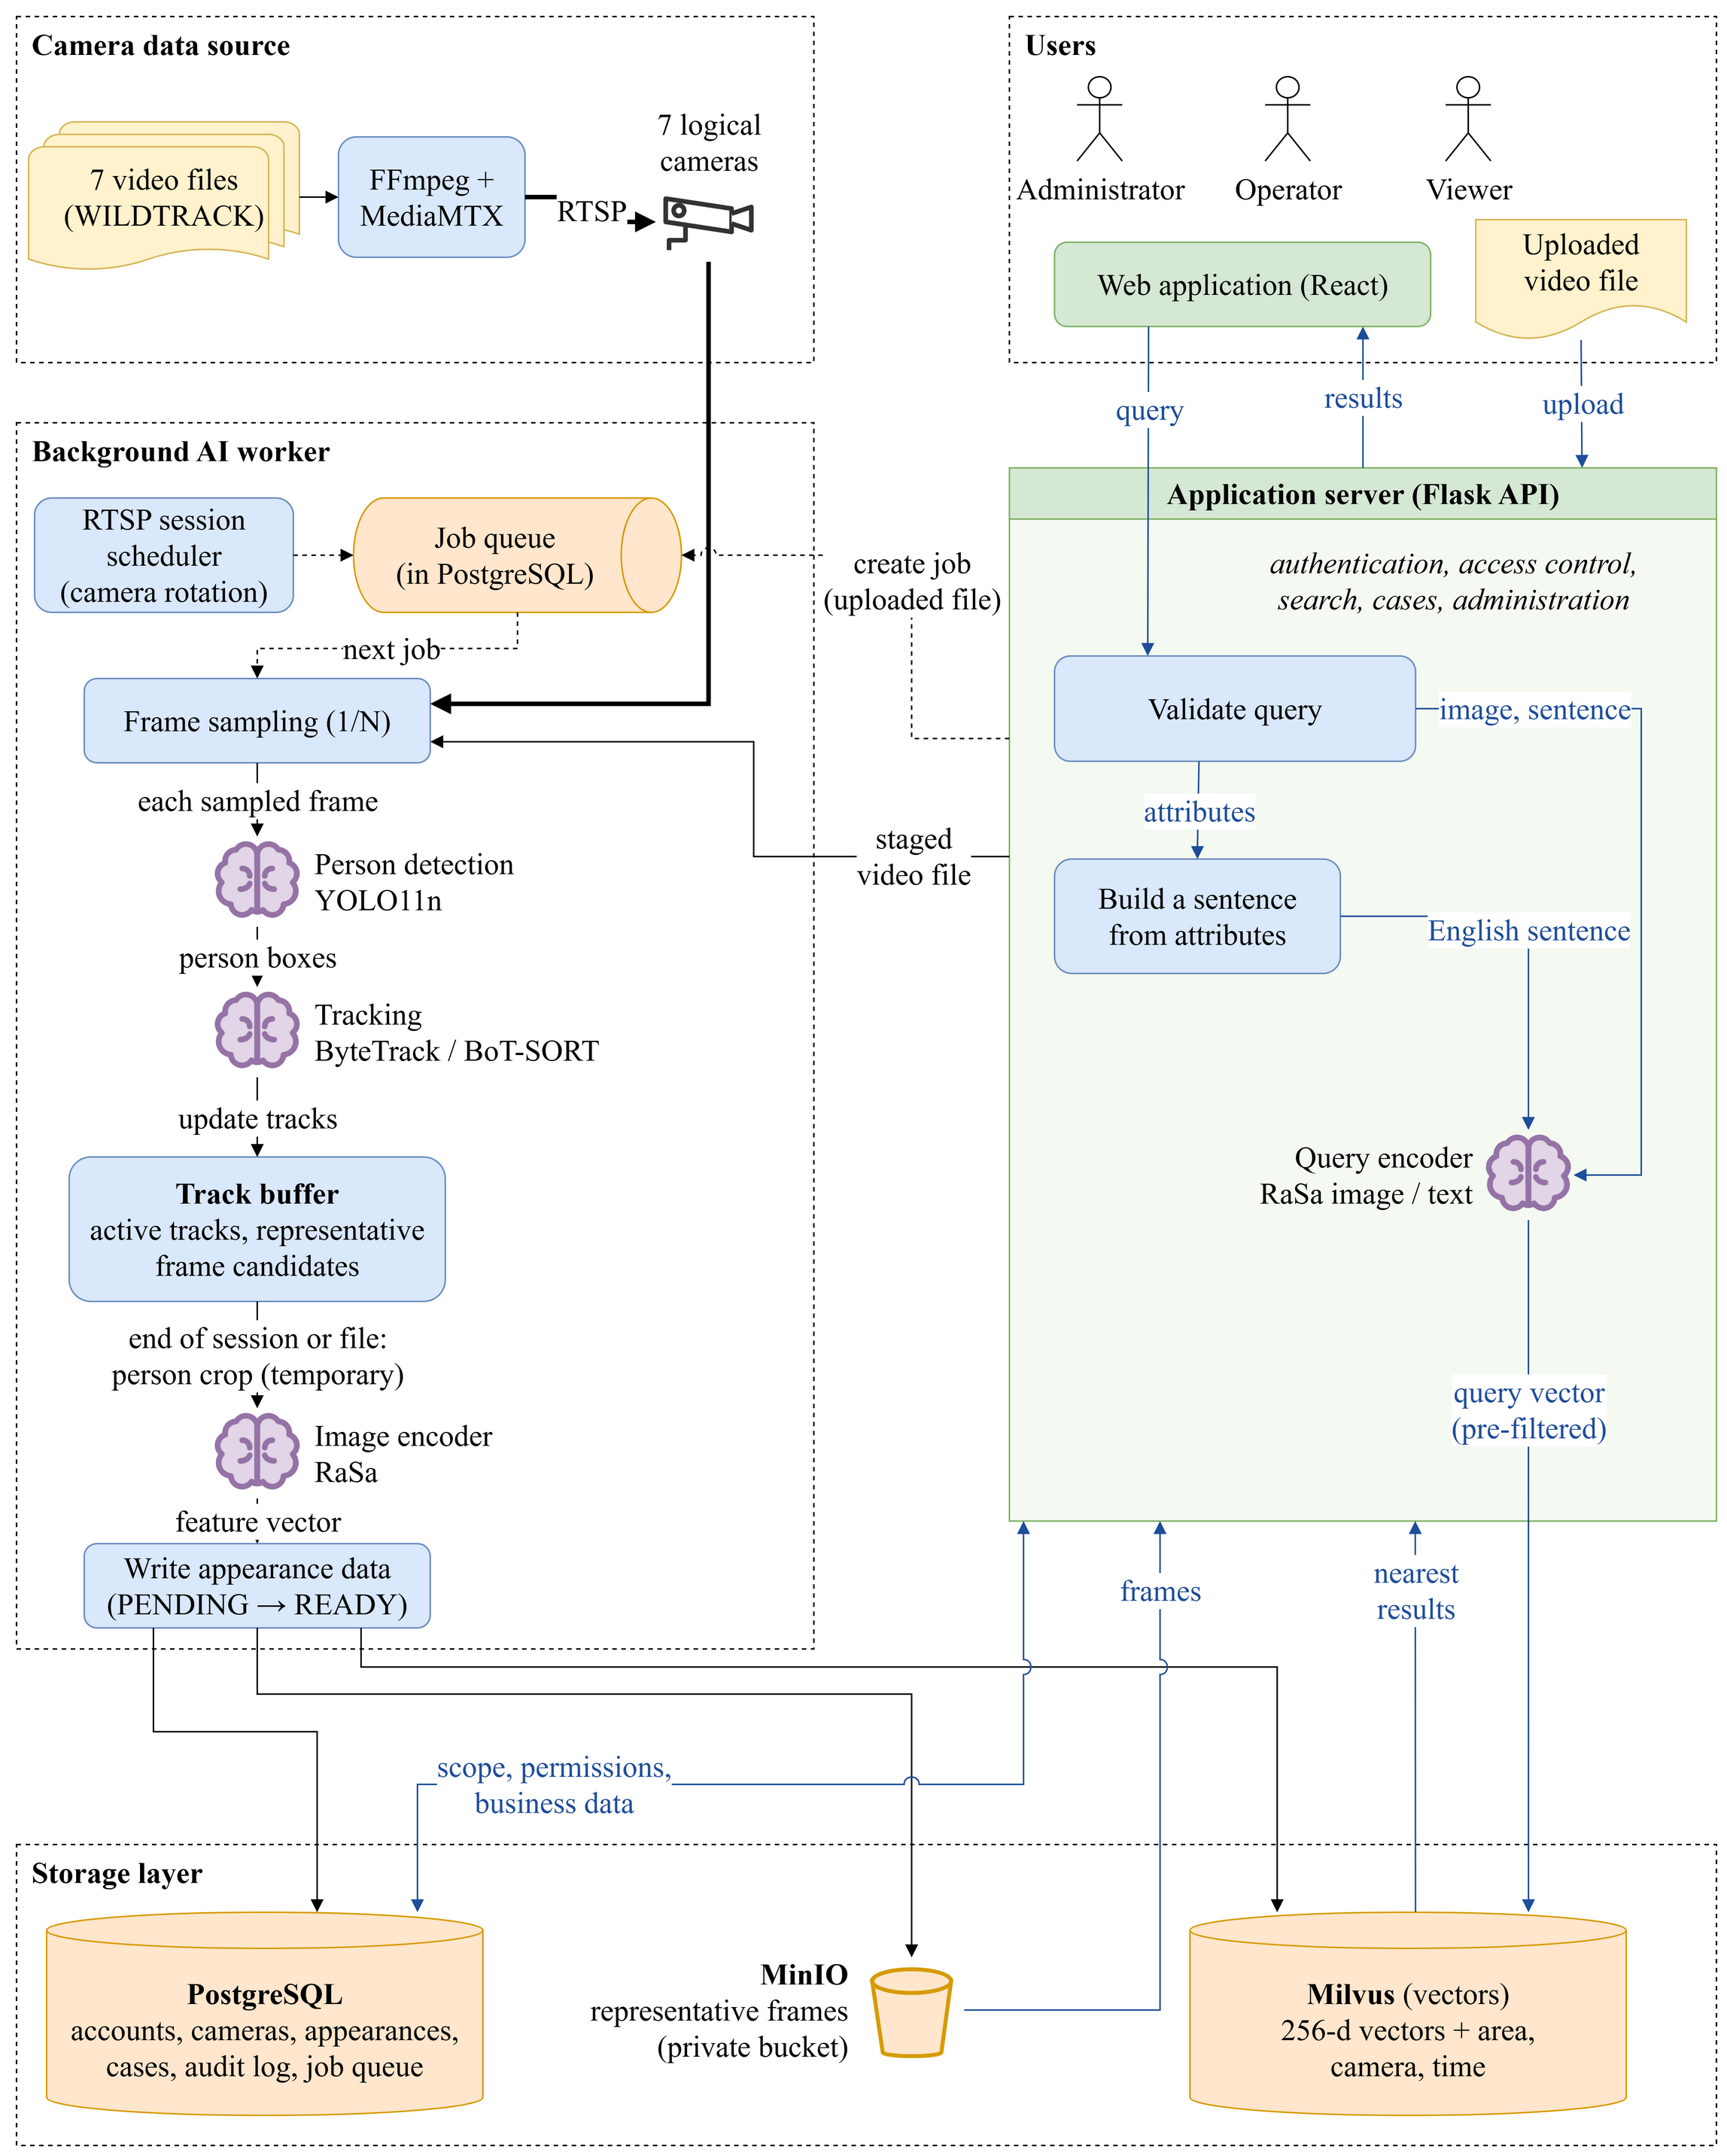
\includegraphics[width=18cm]{H2-kien-truc.png}}
\caption{Overall architecture of the system}
\label{fig:architecture}
\end{figure}

\subsection{Components}
\label{sec:5.1.1}

\begin{itemize}
    \item \textbf{Camera data source.} FFmpeg streams the test videos to a MediaMTX server; each RTSP stream is a logical camera (Section~\ref{sec:3.7.3}), no different from a real IP camera for the system.
    \item \textbf{Web application.} A React interface shared by the three roles; it only talks to the application server, never to a data store.
    \item \textbf{Application server.} A Flask process serves the API and keeps the RaSa encoder loaded for search queries.
    \item \textbf{Background worker.} A separate Python process runs all AI processing: it creates RTSP sessions in rotation among the cameras and runs the queued jobs one by one.
    \item \textbf{Storage layer.} PostgreSQL holds the business data and the job queue, Milvus the feature vectors with their filter fields, and MinIO the representative frame of each appearance.
\end{itemize}

\subsection{Design Principles}
\label{sec:5.1.3}

The main principle is to separate AI processing from the application server. Analysis on the target machine is about seven times slower than real time, so the application server only creates jobs and the background worker runs them. Search stays available during indexing, and analysis errors cannot stop the server.

The job queue is a PostgreSQL table rather than a separate message queue, which means one less component to deploy and keeps job status next to the business data. The worker runs one job at a time, and bounded RTSP sessions rotate among the cameras so that each is analysed in turn without overloading the CPU.

Each store holds one kind of data, linked by a shared appearance identifier, and PostgreSQL is the source of truth (Section~\ref{sec:5.3.4}). Every data access, images included, goes through the application server, so the permission matrix of Section~\ref{sec:4.6} is enforced at one point.

Finally, queries are encoded with the same RaSa weights as the indexed frames, so both lie in one vector space, and RTSP streams and video files share the pipeline after frame reading.

% !TEX root = ../../main.tex
% C5.2 - Main processing flows (translated). Figures H3, H4, H5, H7 are the English versions.
\section{Main Processing Flows}
\label{sec:5.2}

\subsection{Camera Data Processing Flow}
\label{sec:5.2.1}

All analysis is organised into \emph{processing jobs} stored in a queue, each tied to one camera and one data source. For \textbf{automatic RTSP sessions}, when the queue is empty, the scheduler in the background worker chooses a camera that is operational, has AI processing enabled and has an RTSP address, preferring the camera that has waited longest, and creates a session limited to 1,800 source frames, about 30 seconds of video at 60 frames per second; a camera whose last session failed is skipped for 5 minutes so that it does not take the turn of the other cameras. Thanks to the rotation, the cameras are analysed in turn, but between two sessions of the same camera there are periods that are not analysed (Section~\ref{sec:1.4}). For \textbf{uploaded video files}, the application server checks the file, stores it temporarily and creates the corresponding job.

\paragraph{Job life cycle.} Figure~\ref{fig:job-state} shows the states of a job. A new job is \emph{Queued}. When the background worker claims it, the job becomes \emph{Running} with a 60-second lease that is renewed periodically during processing; if the worker stops suddenly and the lease expires, the job can be claimed again. For a video file job, transient errors are retried after a delay, up to three times; an RTSP session that fails ends at once, and the camera is processed again in a later session. A job ends as \emph{Succeeded}, as \emph{Failed} after an unrecoverable error or when the retries are exhausted, or as \emph{Cancelled} when the Administrator cancels it, or when the camera is retired or its AI processing is disabled while the job is queued or running.

\begin{figure}[!htbp]
\centering
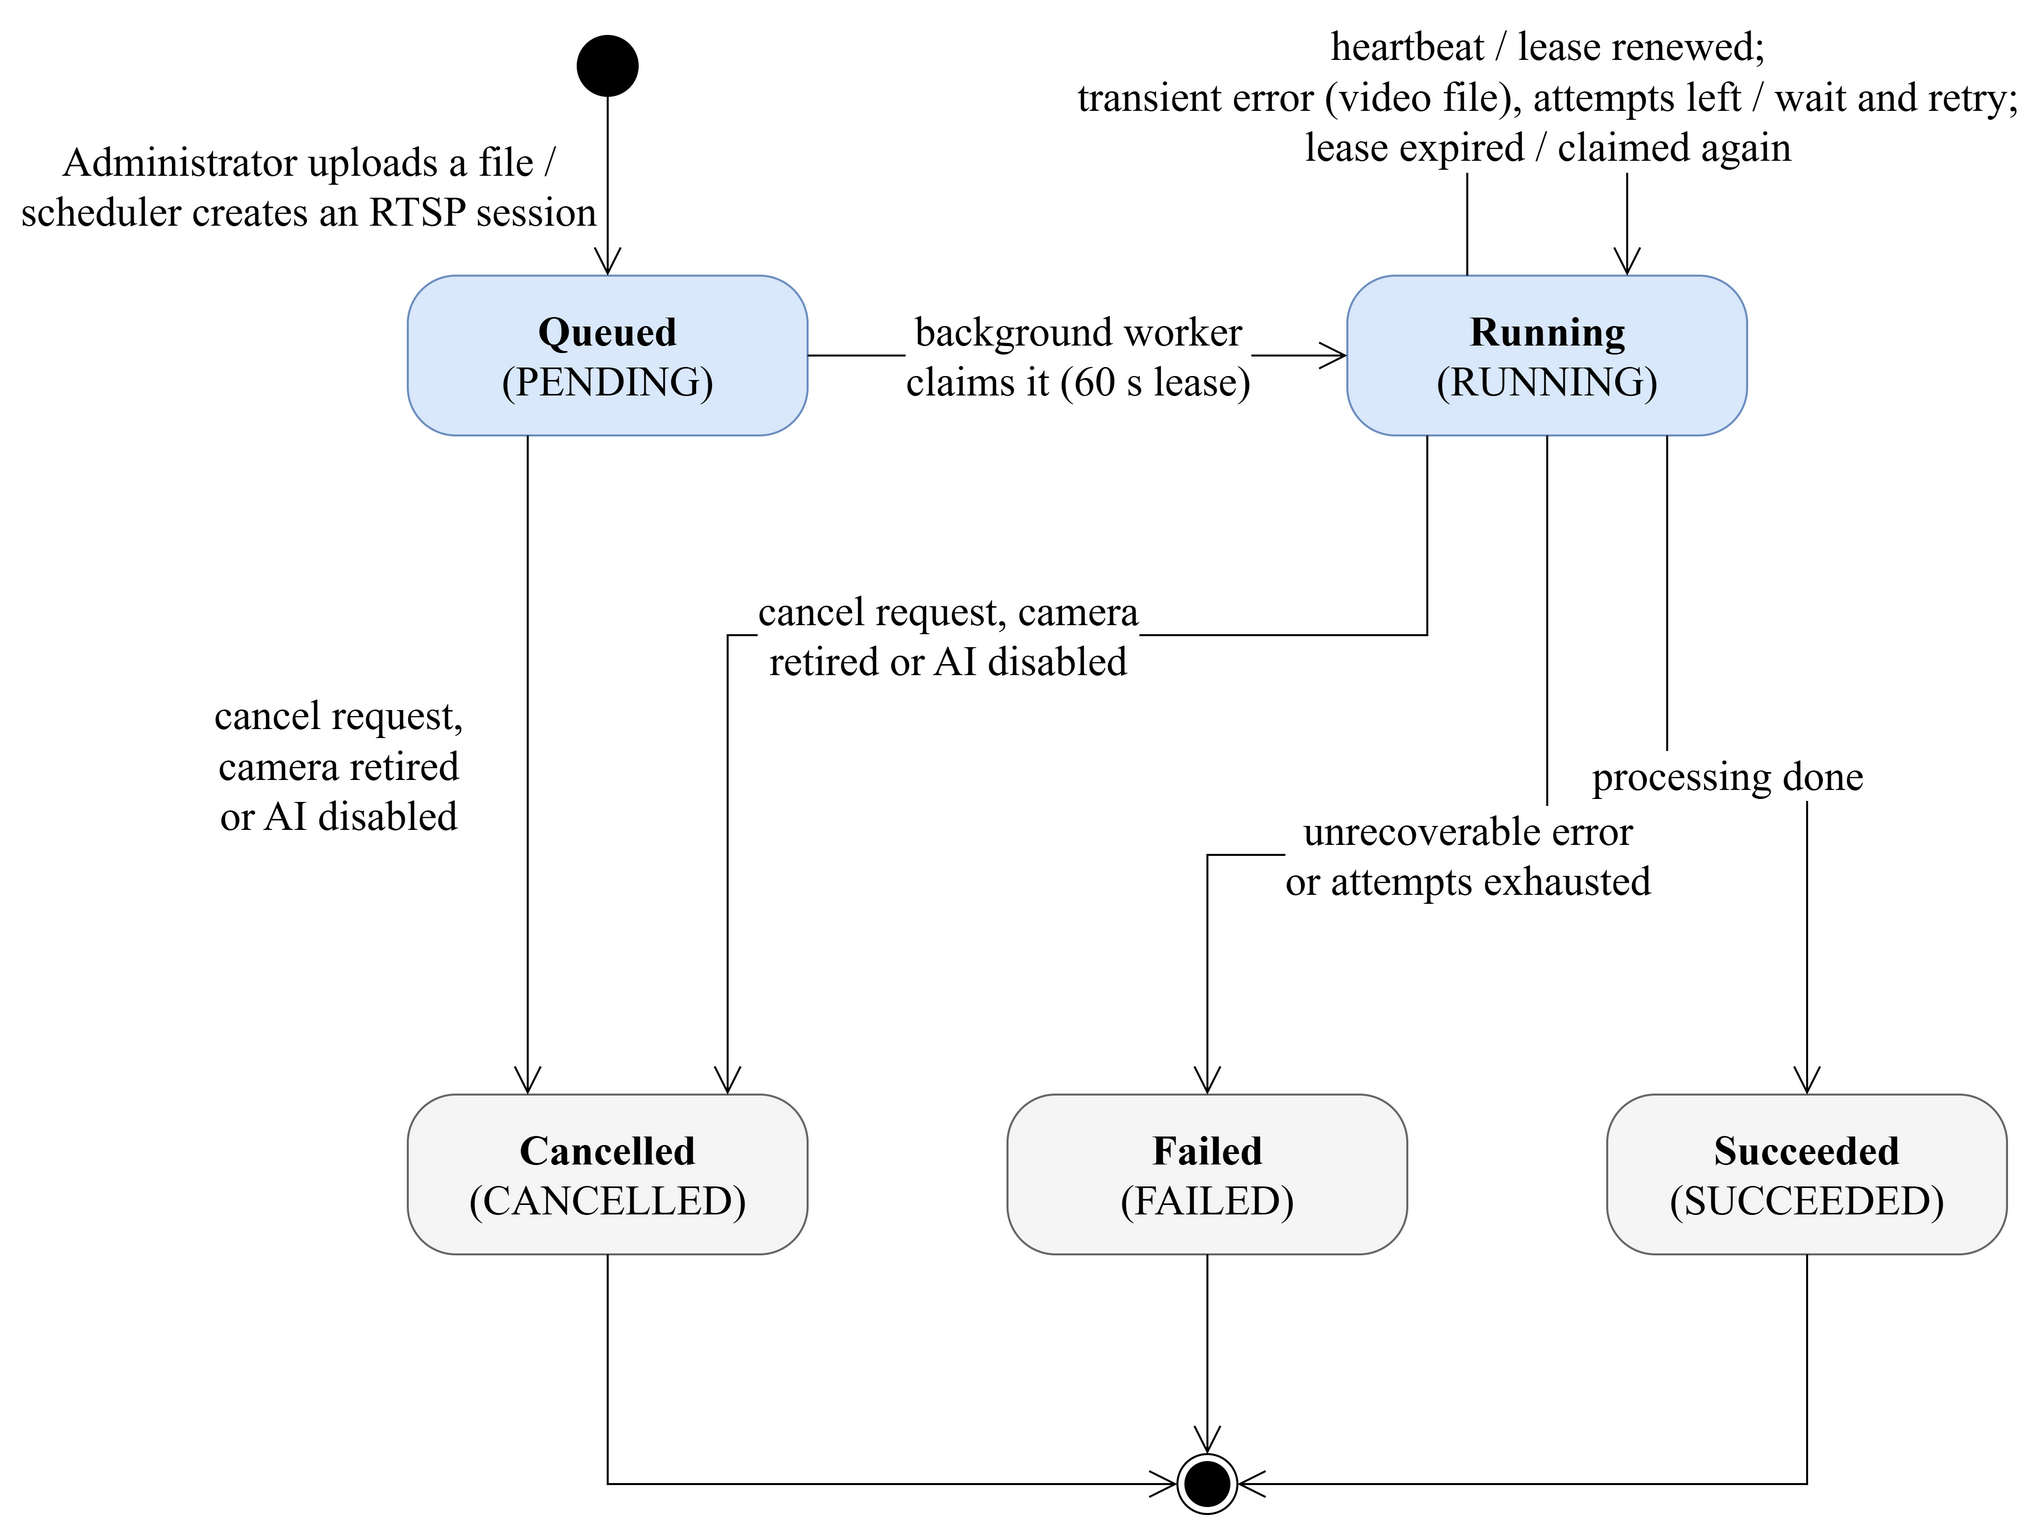
\includegraphics[width=\textwidth]{H7-trang-thai-cong-viec.png}
\caption{State diagram of a processing job}
\label{fig:job-state}
\end{figure}

\paragraph{Processing steps.} Figure~\ref{fig:pipeline-flow} shows the flowchart of one job, which has two phases. In the \emph{per-frame loop}, each frame is read with its index and timestamp (Section~\ref{sec:3.7.4}), and only one in every $N$ frames goes through the Detector and the Tracker. The tracking result updates the \emph{track buffer}, which holds the appearances being tracked with their representative frame candidates, and the system moves on to the next frame. When an appearance ends, its representative frame is chosen and kept in memory. When the source runs out or the session reaches its frame count, the appearances still being tracked are ended as well, and the job moves to the \emph{encode and write} phase: for each appearance, the person region of the representative frame is cropped temporarily in memory, widened by 5\% of the box size on each side, passed through the image encoder to produce the feature vector, and written to the three stores in the order of Section~\ref{sec:5.3.4}. The appearances of a job can therefore only be found after the job has finished its source. For RTSP streams, the source of a job is a session of 1,800 frames, so a camera's data is written session by session: a person appearing in front of the camera can only be searched once the session containing that appearance has been processed. If the job is cancelled or its lease expires while it is reading and analysing the source, none of its appearances is written. Each appearance is written with the version of the Detector-Tracker configuration, the version of the encoder and the sampling interval $N$ used.

\begin{figure}[!htbp]
\centering
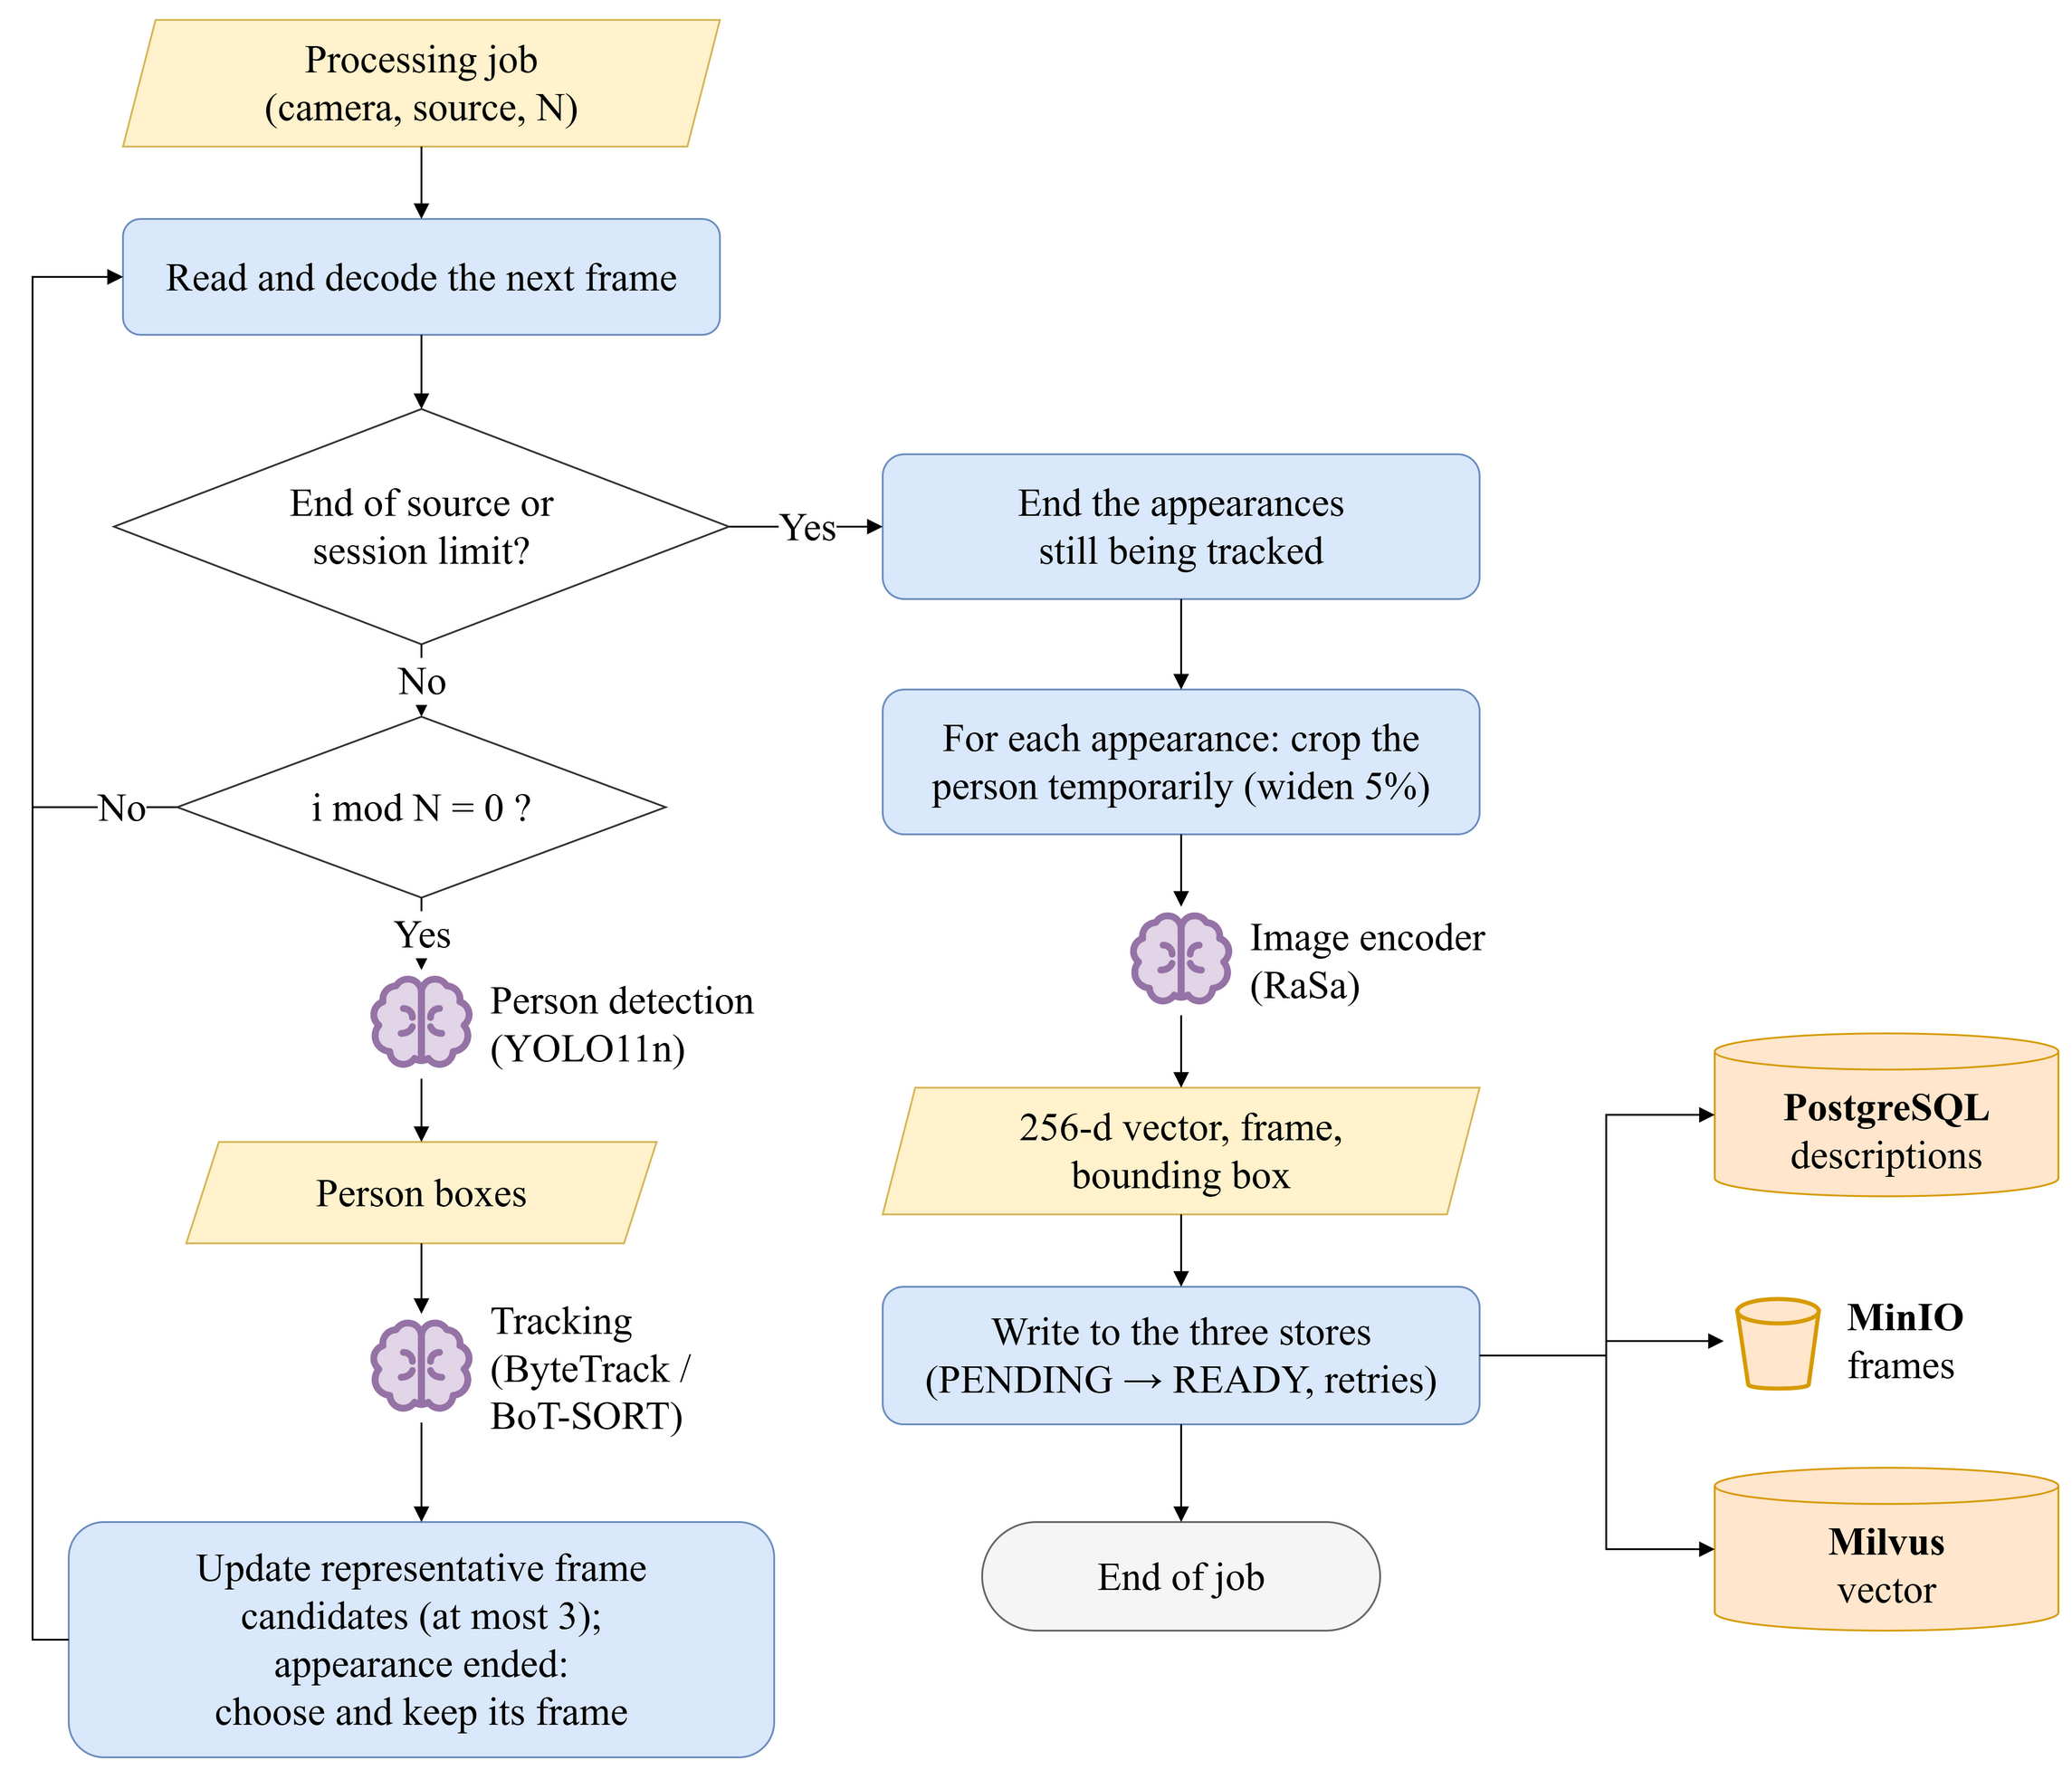
\includegraphics[width=\textwidth]{H3-luu-do-xu-ly-camera.png}
\caption{Flowchart of one processing job}
\label{fig:pipeline-flow}
\end{figure}

\subsection{Representative Frame Selection}
\label{sec:5.2.2}

Each appearance stores only \emph{one} full frame, used both to create the vector and to display the result, so this frame should show the person as clearly as possible. The representative frame selector works as follows:
\begin{itemize}
    \item \textbf{Keep at most three candidates} with the highest scores for each ongoing appearance; the total memory for the candidates of all appearances is limited to 256~MB.
    \item \textbf{Hard filters.} A candidate only passes when its box is at least 24$\times$48 pixels, the person region is sharp enough, the box touches fewer than two edges of the frame and its shape does not change abruptly from the previous observation (area not changing more than 4 times, aspect ratio not changing more than 2.5 times), since an abrupt change usually signals a wrong person or occlusion.
    \item \textbf{The quality score} is a weighted sum of the person's size in the frame (0.30), sharpness (0.25), completeness of the body (0.20), stability relative to the previous observation (0.15) and closeness to the middle of the appearance (0.10), minus penalties when the box touches the frame edges or overlaps other people.
    \item \textbf{Choice at the end.} The highest-scoring candidate among those passing the hard filters is chosen; if none passes, the highest-scoring candidate is still chosen and the appearance is marked low quality instead of being discarded.
\end{itemize}
The criteria and weights were designed empirically, are stored in a configuration file and give deterministic results.

\subsection{Search Flow}
\label{sec:5.2.3}

Figure~\ref{fig:search-sequence} shows the search flow as a sequence diagram.

\begin{figure}[!htbp]
\centering
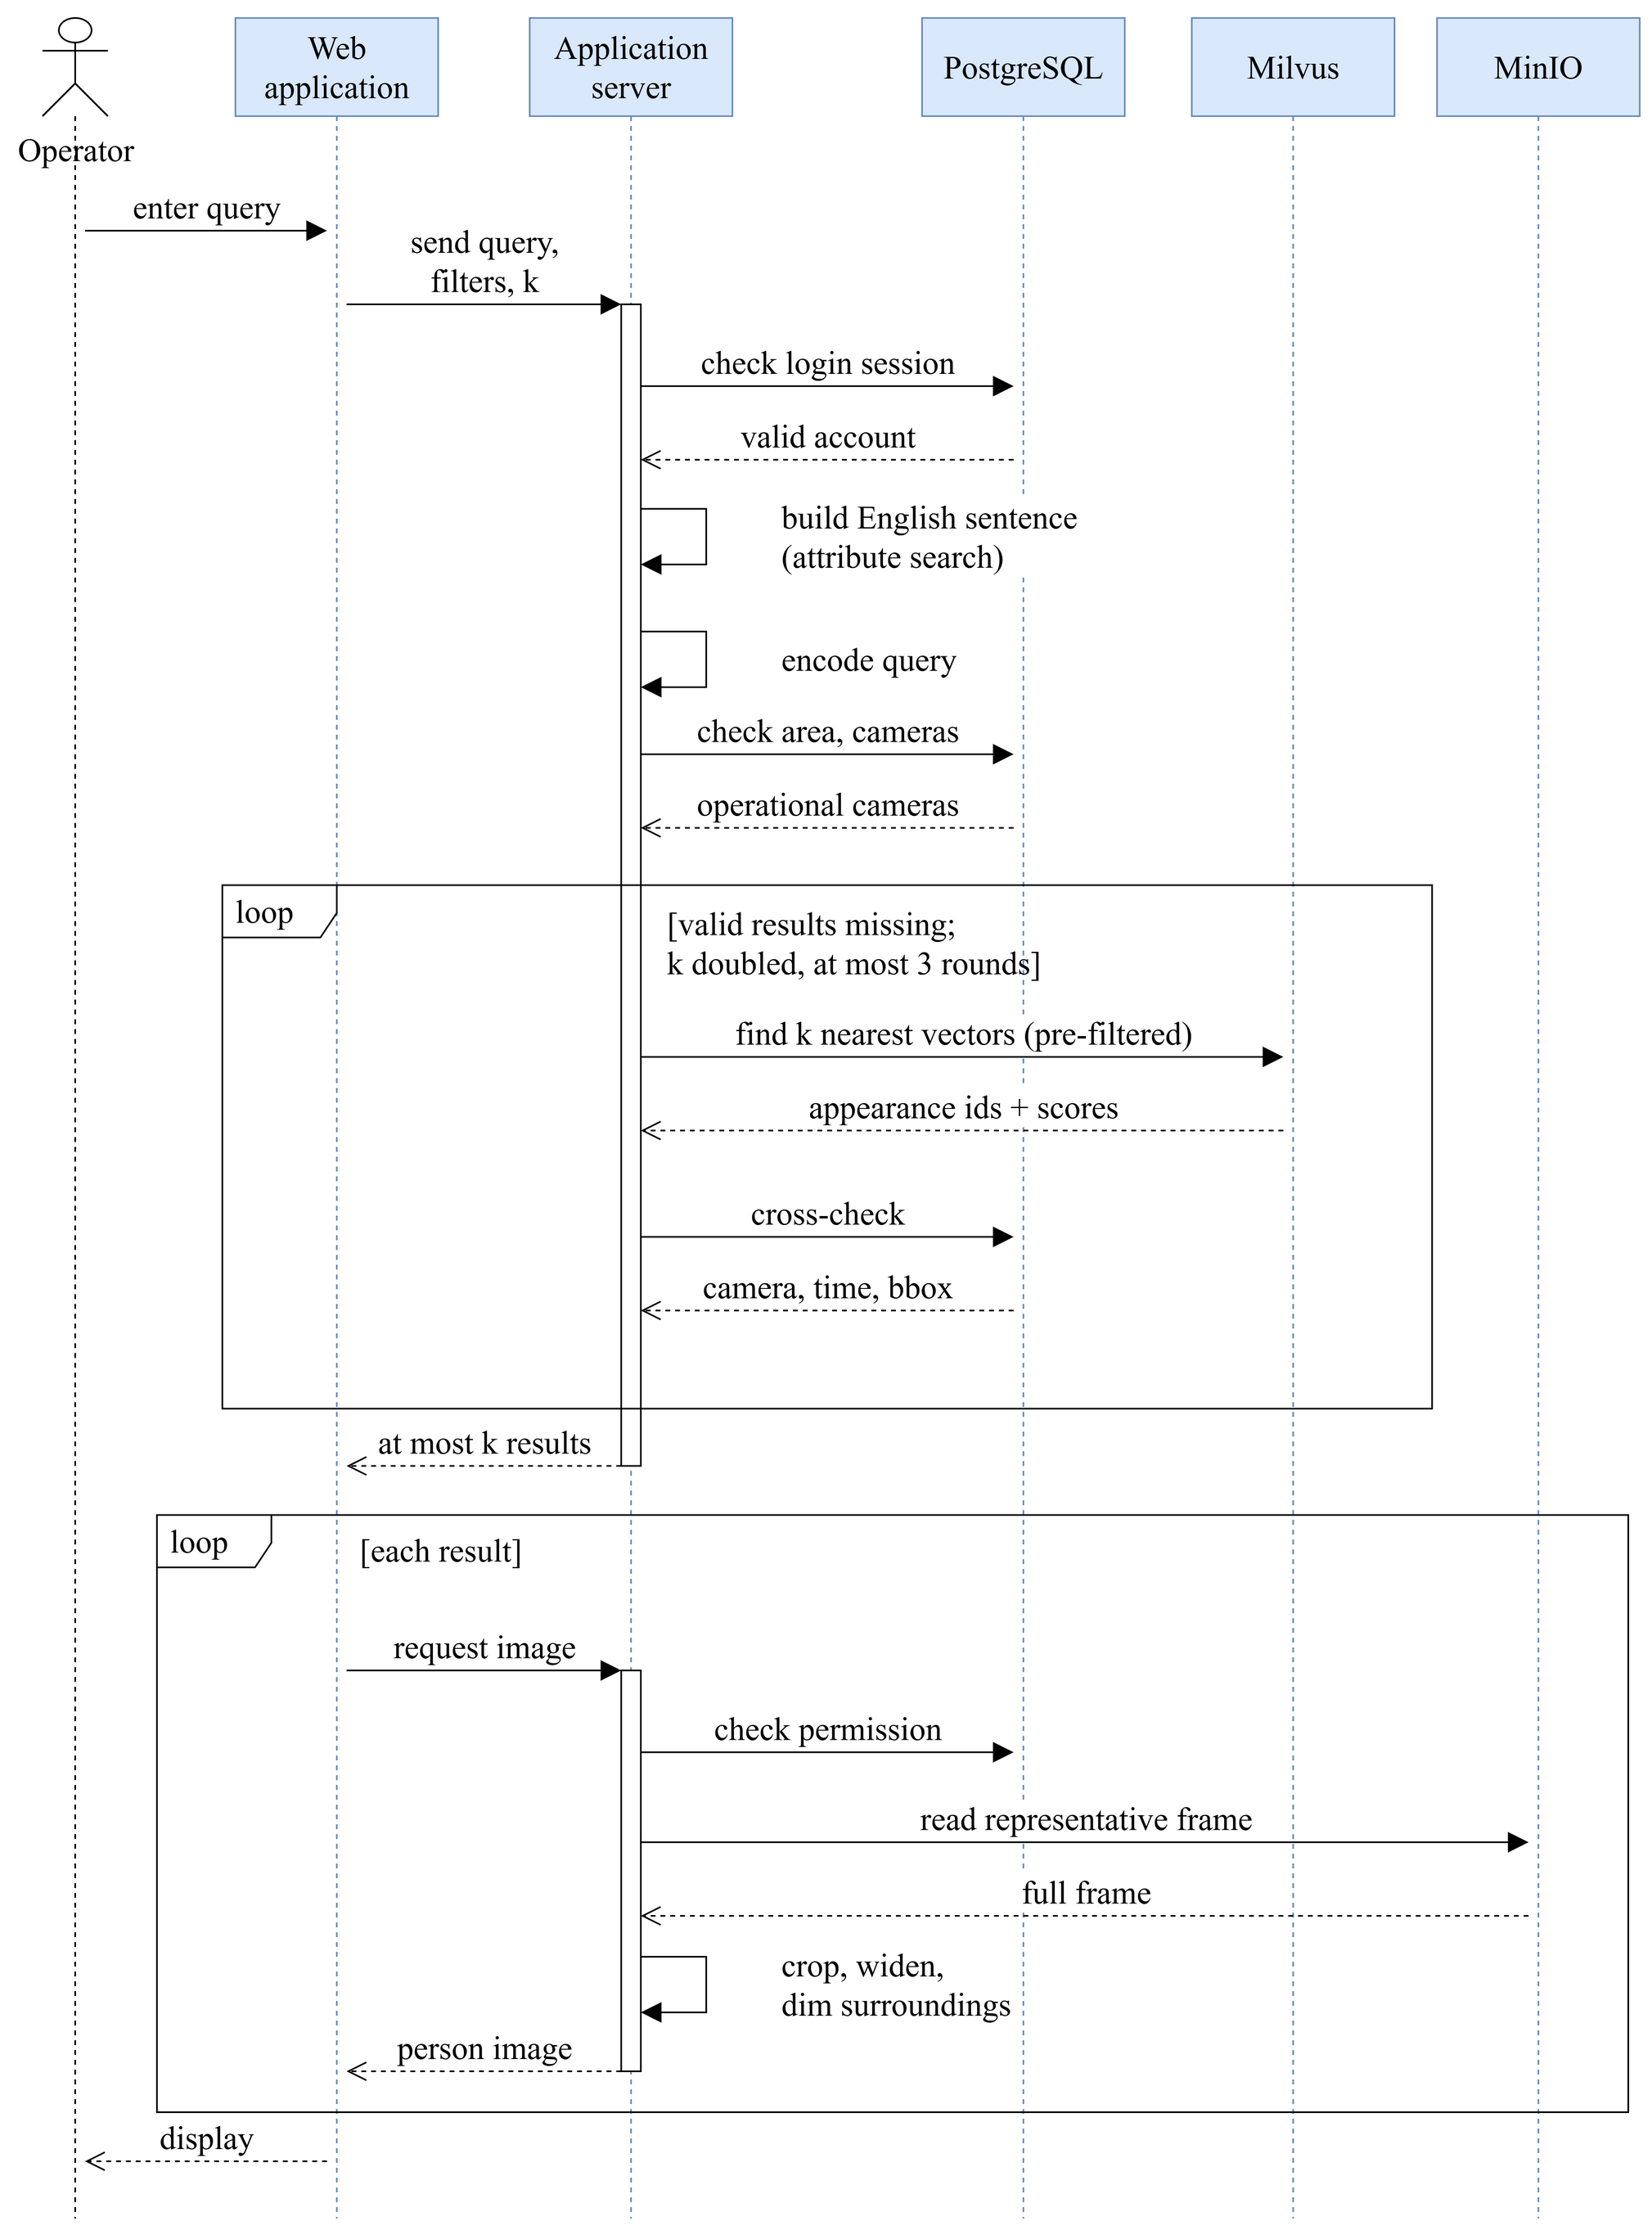
\includegraphics[width=\textwidth]{H4-tuan-tu-tim-kiem.png}
\caption{Sequence diagram of the search flow}
\label{fig:search-sequence}
\end{figure}

The web application sends the query with the camera filter, time range and number of results $k$. The application server then:
\begin{enumerate}
    \item \textbf{validates the input:} a JPEG or PNG image of at most 10~MB; attributes from the allowed list forming a valid combination; $k$ in $\{4, 8, 12, 16\}$;
    \item \textbf{encodes the query:} an image through the image encoder, a description through the text encoder; attributes are combined into an English sentence from a fixed template, for example \emph{``A woman wearing a red jacket and blue jeans, carrying a handbag.''}, and then handled as a description;
    \item \textbf{determines the scope:} the area is taken from the Operator's account; the cameras are those selected, or every operational camera of the area if none is selected; cameras outside the scope are rejected;
    \item \textbf{runs a pre-filtered vector search} in Milvus, checks the results against PostgreSQL and searches again with twice the number when valid results are missing, up to three rounds (Section~\ref{sec:3.6.4}).
\end{enumerate}
The returned list only contains the descriptive information and relevance score of each result. Images are fetched through a separate request for each result, in which the server checks the permission again and renders the person image from the representative frame (Section~\ref{sec:6.3.3}). This keeps the list fast to return and makes every image go through the permission check.

\subsection{Case Management Flow}
\label{sec:5.2.4}

Figure~\ref{fig:case-sequence} shows the flow for saving a search result into a new or existing case, with the option to close the case while saving.

\begin{figure}[!htbp]
\centering
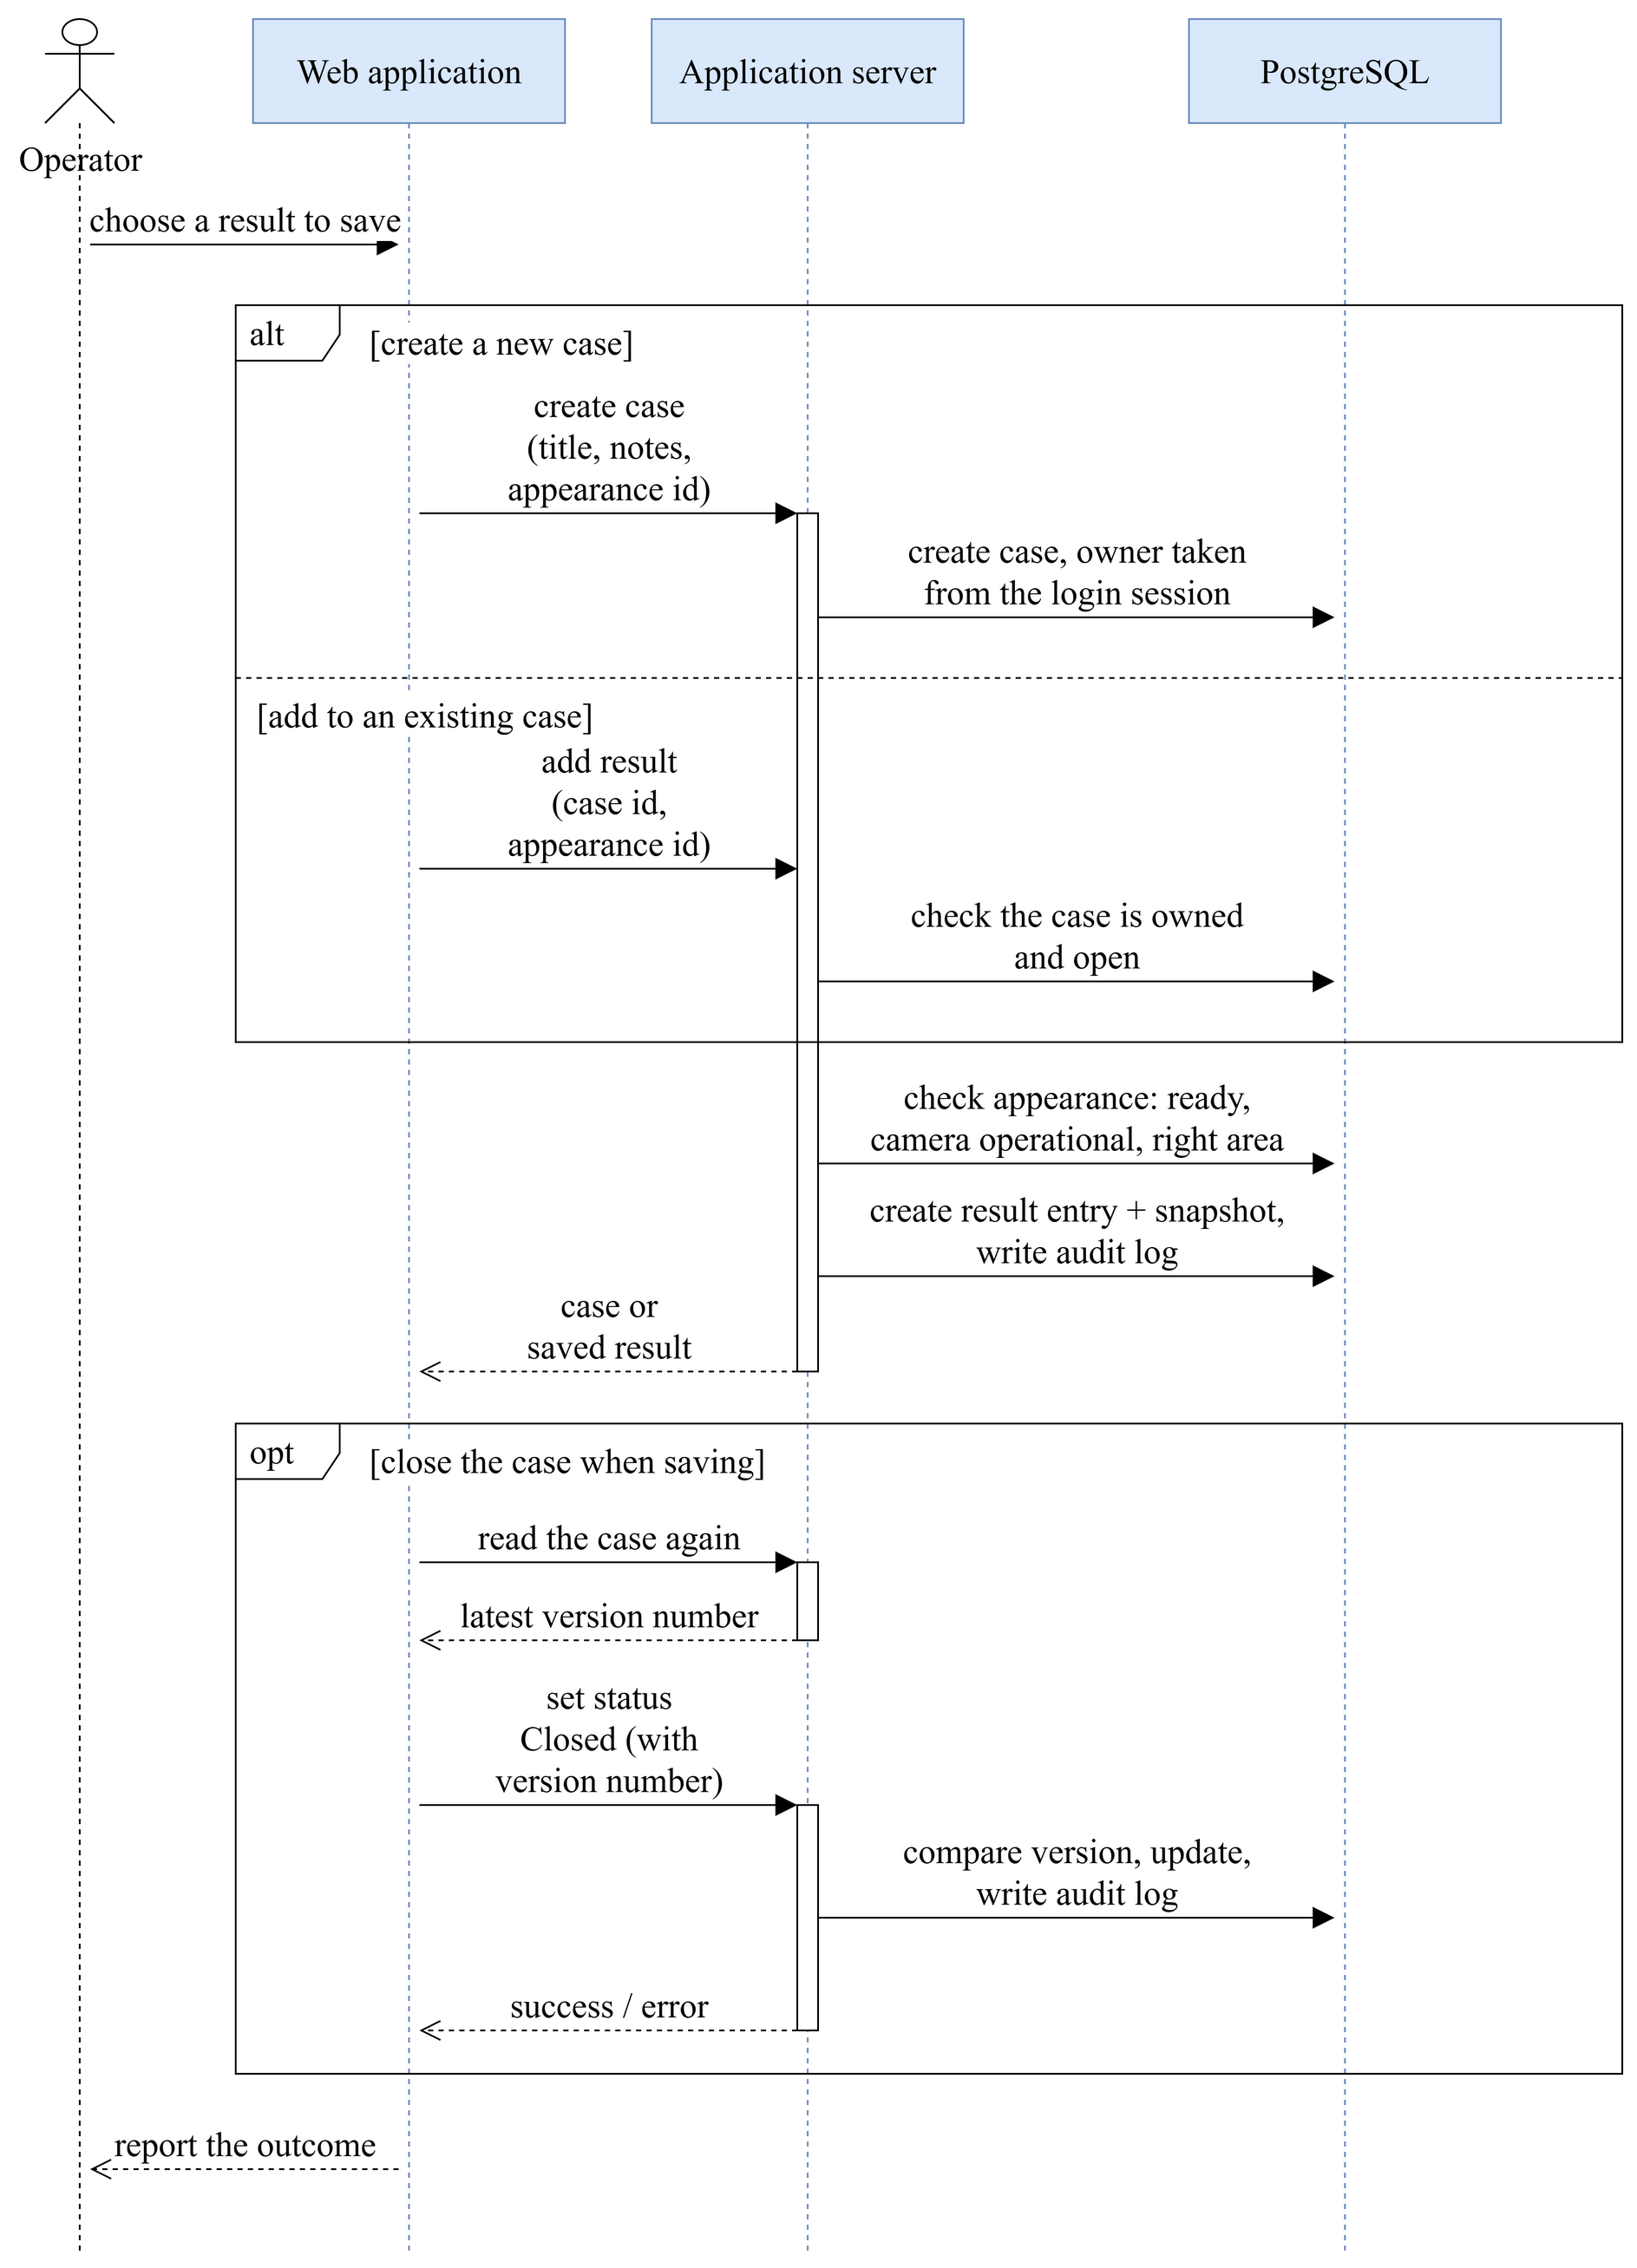
\includegraphics[width=0.95\textwidth]{H5-tuan-tu-vu-viec.png}
\caption{Sequence diagram of saving a result into a case}
\label{fig:case-sequence}
\end{figure}

When saving, the interface only sends the appearance identifier, not the relevance score or display information. The server checks that the appearance is ready and belongs to an operational camera in the Operator's current area, and that the target case is owned by that Operator and open. If valid, the server creates a new result entry with a \emph{snapshot} of the camera name, area name and time of appearance, so that the case still shows correctly if the camera is renamed later or its frame is temporarily unavailable. Each case carries a version number; update requests must include the version being displayed, so concurrent changes from elsewhere are never silently overwritten. The option to close the case is performed by the interface after saving: it reads the case again to get the latest version number, then sends the status change with that version number; if the status change fails, the result is kept and the user is told to close the case again. When a case is opened, images are granted by the right over the case rather than the search right (Section~\ref{sec:4.6}).

% !TEX root = ../../main.tex
% C5.3 - Database design (translated). Matches storage/postgres models and migrations (12 tables), storage/milvus/vectors.py,
% storage/minio/frames.py, services/track_ingestion.py and storage/maintenance_cli.py. Figures H6, H8 are the English versions.
\section{Database Design}
\label{sec:5.3}

\subsection{Relational Database}
\label{sec:5.3.1}

PostgreSQL stores all the business data and is the source of truth for permissions and states. The database has 12 tables in five groups, as in Table~\ref{tab:db-tables}.

\begin{table}[H]
\centering
\caption{Tables of the relational database}
\label{tab:db-tables}
\begin{tabularx}{\textwidth}{|>{\raggedright\arraybackslash}p{3.0cm}|>{\raggedright\arraybackslash}p{5.4cm}|L|}
\hline
\textbf{Group} & \textbf{Tables} & \textbf{Role} \\
\hline
Organisation and access & \texttt{areas}, \texttt{users}, \path{auth_sessions} & Surveillance areas, user accounts, login sessions \\
\hline
Cameras and AI processing & \texttt{cameras}, \path{ai_config_versions}, \path{processing_jobs}, \path{worker_heartbeats} & Logical cameras, versions of the Detector-Tracker-encoder configuration, job queue, background worker status \\
\hline
Search data & \path{person_tracks}, \path{storage_outbox_events} & Descriptions of the appearances; synchronisation events for the other two stores (Section~\ref{sec:5.3.4}) \\
\hline
Cases & \texttt{cases}, \path{case_results} & Cases and their saved results \\
\hline
Traceability & \path{audit_logs} & Audit log, append-only \\
\hline
\end{tabularx}
\end{table}

Figure~\ref{fig:erd} shows the entity-relationship diagram of the 11 tables that have foreign keys, in crow's foot notation; each table only shows its primary key, foreign keys and main attributes. The \path{worker_heartbeats} table has no foreign key and is not drawn.

\afterpage{%
\begin{landscape}
\begin{figure}[p]
\centering
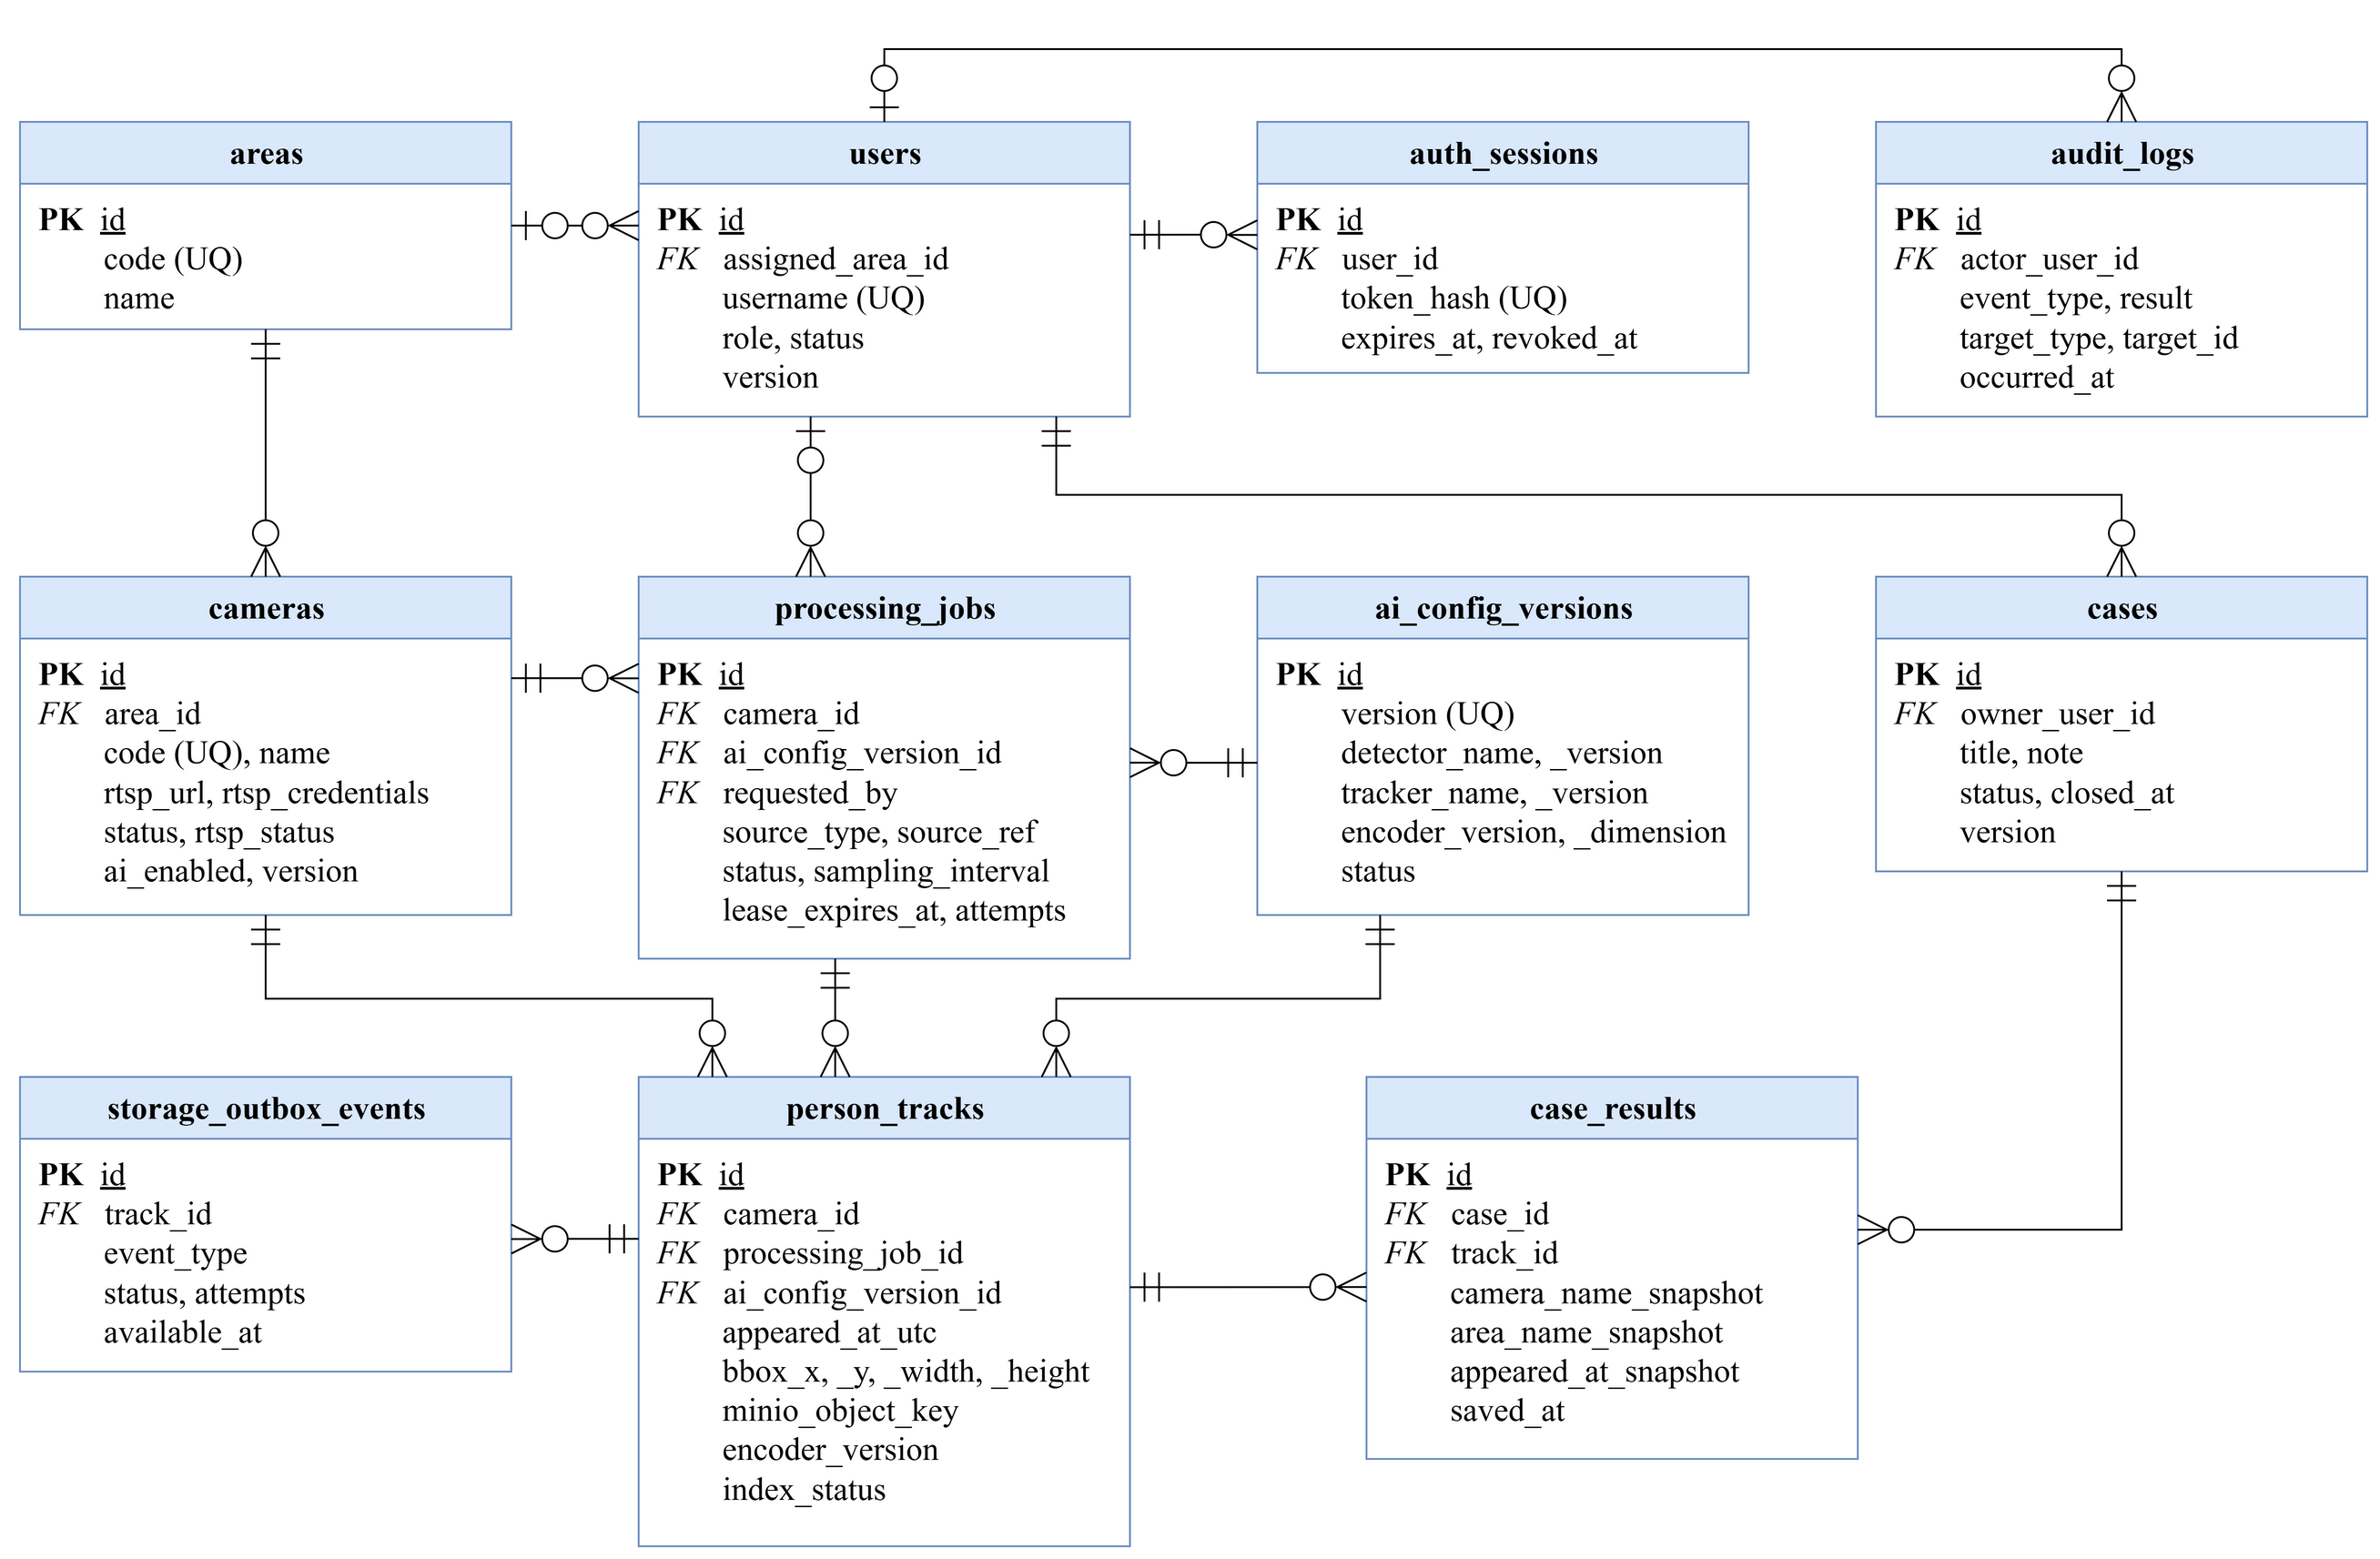
\includegraphics[width=\linewidth,height=0.86\textheight,keepaspectratio]{H8-erd.png}
\caption{Entity-relationship diagram of the relational database}
\label{fig:erd}
\end{figure}
\end{landscape}
}

\paragraph{Relationships.} Most foreign keys are mandatory: each camera belongs to exactly one area, each case has exactly one owner, and each appearance belongs to exactly one camera and was created by exactly one job with one AI configuration version. Three foreign keys may be null: an account only has an area when it is an Operator, a job only has a requester when it was created from an uploaded file, and a log entry may not be tied to a user, for example when it records a technical error. \texttt{cases} and \path{person_tracks} have a many-to-many relationship through \path{case_results}. Each row of this table has its own primary key, stores a snapshot of the information at the time of saving, and has \emph{no} uniqueness constraint on the case-appearance pair, since each save creates a new entry.

\paragraph{Integrity constraints.} Many business rules are expressed directly in the database, so that invalid data cannot be written even if the application layer has a bug:
\begin{itemize}
    \item An Operator account always has an area and the other two roles never do; a case has a closing time if and only if it is \texttt{CLOSED}; only one AI configuration version is \texttt{ACTIVE}; the area code and the area of a camera do not change after creation.
    \item Most foreign keys use the RESTRICT rule, so data that is still referenced cannot be deleted; accounts and cameras are not deleted but change status (\texttt{INACTIVE}, \texttt{RETIRED}). Only login sessions and result entries are deleted with their parent.
    \item An appearance can only be \texttt{READY} when it has the object key, hash and size of its frame and the time its vector was written. No table stores a relevance score.
    \item The \texttt{users}, \texttt{cameras} and \texttt{cases} tables have a version column to prevent overwriting on concurrent updates (Section~\ref{sec:5.2.4}); the requester-idempotency key pair of \path{processing_jobs} is unique, so a repeated upload request creates no additional job.
\end{itemize}
Indexes are also created for frequent queries, such as appearances by camera and time (with a separate index containing only ready appearances), cases by owner, and log entries by actor.

\subsection{Feature Vector Storage}
\label{sec:5.3.2}

Milvus serves a single purpose: quickly finding the vectors closest to the query vector within a filtered scope; all other information and every permission decision live in PostgreSQL.

\paragraph{One collection per encoder version.} Milvus organises data into \emph{collections}, similar to tables. The system creates a separate collection for each encoder version, for example \path{person_track_embeddings_rasa_cuhk_pedes_v1}, because vectors from two versions belong to two representation spaces that cannot be compared. A fixed alias always points to the collection of the version in use; when the background worker starts, the dimension of the collection is checked against the configuration. Each appearance corresponds to one record with the fields of Table~\ref{tab:milvus-schema}.

\begin{table}[H]
\centering
\caption{Schema of the Milvus collection of feature vectors}
\label{tab:milvus-schema}
\begin{tabularx}{\textwidth}{|>{\raggedright\arraybackslash}p{4.2cm}|>{\raggedright\arraybackslash}p{3.7cm}|L|}
\hline
\textbf{Field} & \textbf{Type} & \textbf{Meaning} \\
\hline
\path{track_id} & VARCHAR(36), primary key & Appearance identifier, the same as the primary key of \path{person_tracks} \\
\hline
\path{embedding} & FLOAT\_VECTOR, 256 dimensions & Feature vector, L2-normalised \\
\hline
\path{area_id}, \path{camera_id} & VARCHAR(36) & Area and camera, used for scope filtering \\
\hline
\path{appeared_at_epoch} & INT64 & Time of appearance (Unix seconds), used for time filtering \\
\hline
\path{encoder_version} & VARCHAR(64) & Version of the encoder that produced the vector \\
\hline
\path{index_status} & VARCHAR(16) & Readiness; only \texttt{READY} records are searched \\
\hline
\end{tabularx}
\end{table}

The area, camera and time fields are copied from PostgreSQL so that Milvus can pre-filter before searching (Section~\ref{sec:3.6.3}); since the area of a camera does not change after creation, this copy cannot diverge. The operational status of a camera, by contrast, changes with the Administrator's actions and is not copied: each search takes the list of operational cameras from PostgreSQL and puts it in the filter, so the data of a retired camera is hidden immediately without updating Milvus.

\paragraph{Index and operations.} The vector field has an HNSW index with the inner-product metric, $M = 16$, \textit{ef\-Con\-struc\-tion}~$= 128$, and $\mathit{ef} = 64$ at search time (Section~\ref{sec:3.6.4}). Vectors are written with an \emph{upsert} keyed by the appearance identifier, so retries create no duplicate records, and are checked for the right dimension, the absence of invalid values and unit length before writing or searching. Every operation uses strong consistency, so a vector just written appears in the very next search.

\subsection{Frame Storage}
\label{sec:5.3.3}

Each appearance has exactly one image file in MinIO: the representative full frame, stored as JPEG at quality 90; PostgreSQL only stores the object key, hash and file size. The system does not store cropped person images as separate files: the person image in the result list is rendered from the full frame and the bounding box on request (Section~\ref{sec:6.3.3}). One file therefore serves both views, the cropping can change without regenerating data, and no standalone person images exist that could be copied out of control. The original video is not stored.

The key of each file is derived deterministically from the appearance, following the pattern
\begin{center}
\texttt{tracks/v1/}\allowbreak \textit{camera code}\texttt{/}\allowbreak \textit{year}\texttt{/}\allowbreak \textit{month}\texttt{/}\allowbreak \textit{day}\texttt{/}\allowbreak \textit{appearance id}\texttt{/}\allowbreak \texttt{representative.jpg}
\end{center}
so a retry rewrites the same file instead of creating a new one; the versioned prefix allows the layout to change later, and grouping by camera and day makes clean-up by camera or time range easy.

Before writing, the file is checked for the right format, a size of at most 20~MB and dimensions matching its description; its SHA-256 hash is stored in both MinIO and PostgreSQL. A write to an existing key with the same hash reuses the existing file, and one with a different hash is rejected as a conflict; on reading, the hash is recomputed to detect corruption. The files live in a private bucket, the application accesses it with an account that only has rights on that bucket, and the browser never receives a direct address to MinIO.

\subsection{Consistency Across the Stores}
\label{sec:5.3.4}

An appearance is stored as three parts in three stores, linked by the same identifier. The three stores share no transaction, so the process may stop midway or a store may be temporarily unreachable. The system guarantees that incomplete data never appears in search results and can be completed or detected later.

\paragraph{Appearance states.} Each appearance record has a synchronisation state, with the allowed transitions of Figure~\ref{fig:track-state}. Only appearances in the \emph{Ready} state can be searched; transitions not shown in the figure are rejected by the application layer.

\begin{figure}[!htbp]
\centering
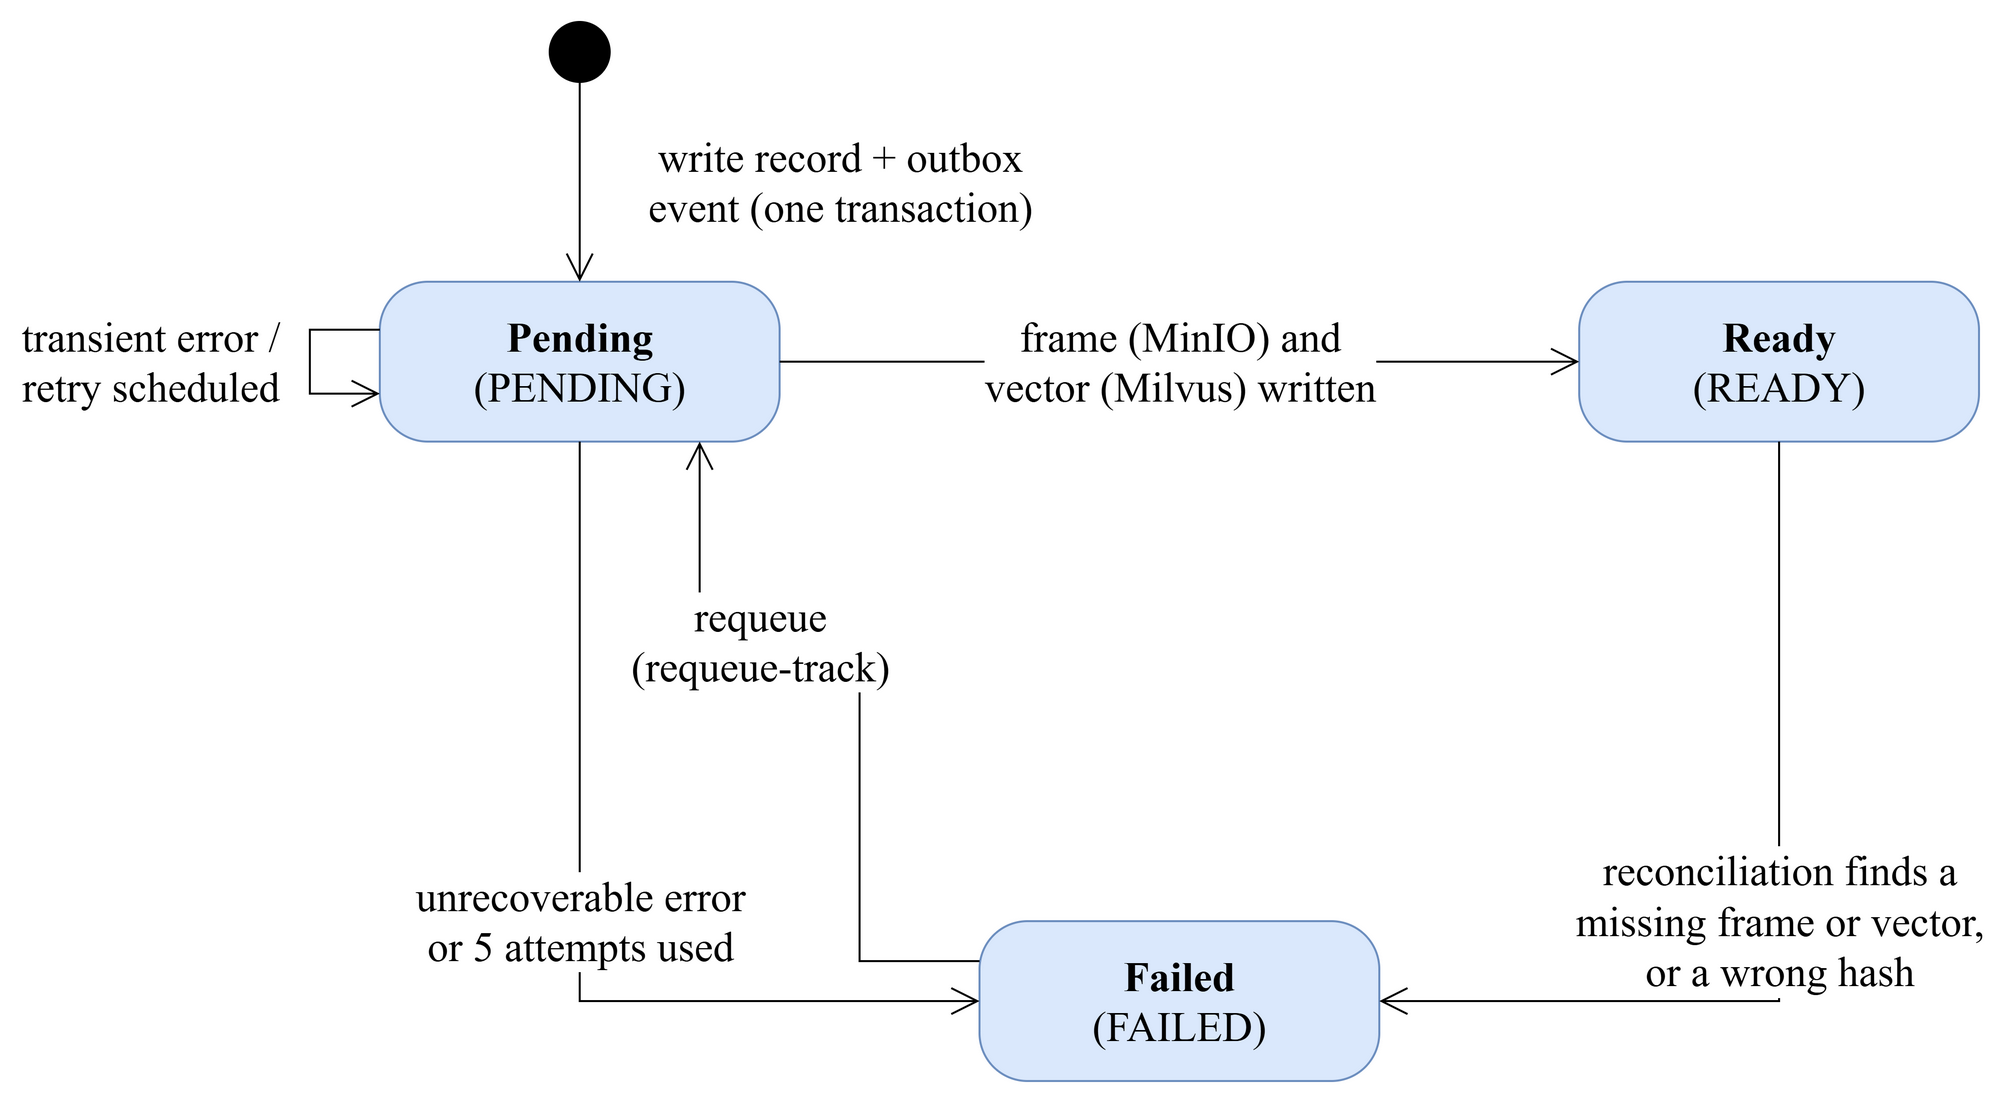
\includegraphics[width=\textwidth]{H6-trang-thai-lan-xuat-hien.png}
\caption{State diagram of an appearance}
\label{fig:track-state}
\end{figure}

\paragraph{Write order.} An appearance is written in a fixed order:
\begin{enumerate}
    \item In \emph{one} PostgreSQL transaction, create the record in the \emph{Pending} state and an event in \path{storage_outbox_events} holding everything that must be written to the other two stores, the vector included. This is the \emph{transactional outbox} pattern: the intent to write to another system is stored in the same transaction as the main data.
    \item Write the frame to MinIO under its deterministic key.
    \item Write the vector to Milvus, then read it back to confirm the record exists with the right area and camera.
    \item In a new transaction, move the record to \emph{Ready}, store the hash and size of the frame and the time the vector was written, and mark the outbox event as done.
\end{enumerate}
Because PostgreSQL is always written \emph{first}, every frame and vector can be matched with a known record, and anything without a matching record is orphaned data. Because the \emph{Ready} state is set \emph{last}, an appearance can only be found once all its data is present. Steps 2 and 3 can both be repeated safely thanks to the deterministic key and the upsert.

\paragraph{Error handling and maintenance tools.} If step 2 or 3 fails with a transient error, the record stays \emph{Pending} and the outbox event is scheduled for retry, with a delay starting at 2 seconds, doubling each time, up to 300 seconds. After five unsuccessful attempts, or on an unrecoverable error such as a hash conflict, the record moves to \emph{Failed} and the incident is written to the audit log. Since the outbox event holds all the data, a retry does not need to rerun the video analysis. Operators also have a command-line tool to complete pending appearances; to reconcile the three stores, finding records pending for too long, ready records missing their frame or vector, and orphaned data (by default it only reports; on request it quarantines broken records and deletes orphans); to move a failed appearance back to pending; and to rebuild the Milvus data from the outbox events. These commands are currently run by hand.

\paragraph{Protection at search time.} Even when the three stores are temporarily out of sync, users never see wrong data: every result returned by Milvus is checked again against PostgreSQL, and results that do not exist or are outside the permitted scope are removed before being shown (Section~\ref{sec:3.6.4}).

% !TEX root = ../../main.tex
% C5.4 - API design (translated). Matches backend/src/person_search/api.
\section{Application Programming Interface Design}
\label{sec:5.4}

The web application and the application server communicate entirely through a REST-style application programming interface (API). Every business API lives under the prefix \path{/api/v1} and names resources with plural nouns, such as \path{/cases}. APIs reserved for the Administrator live under \path{/admin}. Data is exchanged as JSON, except query images and video files, which are sent as \texttt{multipart/form-data}. State transitions with a business meaning, such as locking an account or retiring a camera, are designed as explicit actions, for example \texttt{POST} \path{/admin/cameras/{id}/retire}, so that each one is checked and logged separately.

Every error is returned in one format with a stable \emph{error code} for the interface to handle programmatically, a \emph{message} in Vietnamese for display, \emph{details} such as per-field errors, and a \emph{request identifier} for matching with the server log. HTTP status codes are used with their standard meaning: 401 when not logged in or the session has expired, 403 when the role is not allowed, 404 when the resource does not exist or is outside the permitted scope, 409 on a conflict with the current state, 422 for invalid data and 429 when the call limit is exceeded.

To prevent overwriting, requests that update accounts, cameras and cases must include the version number the interface holds. If the data has been changed elsewhere, the server returns 409 instead of overwriting. A video upload request may carry an idempotency key, so resending it creates no additional job. Uploading a video is also asynchronous: the server only creates the job and returns 202 immediately, and the interface follows the progress through the jobs API instead of keeping the request open for the whole analysis.

For access control, no API takes the Operator's area or the case owner as a parameter. The server determines these values from the login session, so editing a request in the browser cannot widen the rights. Search and case responses only contain descriptive information, and images are fetched through separate paths. Images of search results and images of saved results use two different sets of paths, matching the two grounds for viewing images in Section~\ref{sec:4.6}.

Besides the business APIs, the server has three health-check paths (\path{/health/live}, \path{/health/ready}, \path{/health/storage}) for deployment and monitoring.

% !TEX root = ../../main.tex
% C5.5 - Security and access control design (translated). Matches auth/*, api/security.py, api/rate_limit.py, services/*.
% Note: refresh() sets a new expiry of now + 12 h (architect.md section 13 #8, spec follows the application).
\section{Security and Access Control Design}
\label{sec:5.5}

This section presents the mechanisms implementing the security requirements of Section~\ref{sec:4.3.1} and the permission matrix of Section~\ref{sec:4.6}, following the principle of \emph{defence in depth}: each request is checked in turn for its login session, its role and its data scope, and the database constraints are the last layer that keeps invalid data from being written.

\subsection{Authentication and Sessions}
\label{sec:5.5.1}

Passwords are hashed with Argon2 and are at least 8 characters long. When the username does not exist, the system still verifies against a dummy hash and returns the same error message as for a wrong password, so that neither the response time nor the error content reveals which usernames exist; every failed login is written to the audit log.

On a successful login, the server generates a random 32-byte session token and sends it in a cookie with the \texttt{HttpOnly} attribute, so that JavaScript on the page cannot read it, \texttt{SameSite=Lax}, so that the browser does not send the cookie with data-changing requests coming from another site, and \texttt{Secure} when deployed over HTTPS. The database only stores the SHA-256 hash of the token, so even if the session table leaks, an attacker has no valid token. On each request, the server answers 401 if the session has been revoked, is more than 12 hours old since it was issued, or has been inactive for more than 30 minutes, and revokes the session immediately if the account has been locked or deactivated or is an Operator without an area. While the user is actually active, the interface refreshes the session periodically; each refresh issues a new token whose 12-hour limit counts from the refresh and revokes the old one, so a leaked token is only valid for a short time.

\subsection{Cross-Site Request Forgery Protection}
\label{sec:5.5.2}

Since the browser sends the session cookie automatically, a malicious website could try to make the user's browser send requests to the system without the user knowing (a CSRF attack). Besides the \texttt{SameSite} attribute, every data-changing request must carry an \texttt{X-CSRF-Token} header containing an anti-forgery token, computed with HMAC-SHA256 from the session token and returned to the interface at login; another website cannot read this token and therefore cannot build a valid request. The server only allows the configured origins to call the API with cookies (CORS), and every response carries security headers such as disabling content-type sniffing, forbidding the page from being framed by another site and disabling caching of API responses.

\subsection{Access Control}
\label{sec:5.5.3}

Access control is enforced on the server in three layers. First, each API declares the roles allowed to call it; requests from other roles are rejected with 403 before any business processing. Second, the business layer checks the rights on each object: cameras and appearances must belong to the Operator's current area and the camera must be operational, a case must be owned by that Operator, and images are granted on one of the two grounds of Section~\ref{sec:4.6}; the area and the owner are always taken from the login session. Third, the database constraints keep invalid data from being written even if the business layer has a bug.

For objects outside the scope, the server returns 404 rather than 403: with 403, a user could infer that an object exists by trying identifiers one by one. Hiding the functions of other roles in the interface is only a convenience and is not considered an access control measure.

\subsection{Data Protection and Abuse Limitation}
\label{sec:5.5.4}

The credentials in an RTSP address are separated, encrypted with the Fernet symmetric encryption scheme using a key configured through an environment variable, and only decrypted at connection time; they are never returned to the interface or written to logs. Since the connection check makes the server connect to an address entered by the user, the system only accepts IP addresses within the camera network ranges declared at deployment and always rejects loopback, link-local and multicast addresses, so that the function cannot be abused to probe other machines on the internal network (an SSRF attack).

Resource-intensive or probe-prone functions are limited in calls per minute: login 10 times per IP address-username pair, and search 30 times, video upload 10 times, camera connection check 10 times and AI check 6 times per account. When the limit is exceeded, the server returns 429 with the time to wait. The counters live in the memory of the server process, which suits the project's single-process deployment. Uploaded data is also checked before processing: query images must be JPEG or PNG, at most 10~MB and 24 megapixels, and video files at most 500~MB with a valid format signature. File names sent by users are never used as storage paths.

% !TEX root = ../../main.tex
% C5.6 - User interface design (translated). Figure H12 is the English version. Screen names are the English meaning of the Vietnamese UI.
\section{User Interface Design}
\label{sec:5.6}

The interface was designed directly in the web application, without a mock-up stage; Section~\ref{sec:6.3} shows the main screens.

\subsection{Screen Structure by Role}
\label{sec:5.6.1}

Each role lands on its own home page and only sees its own screens (Figure~\ref{fig:screen-flow}). In the figure, bold arrows mark the page opened after login, dashed frames are dialogs, and screens of one role are linked through the left-hand menu.

\begin{figure}[!htbp]
\centering
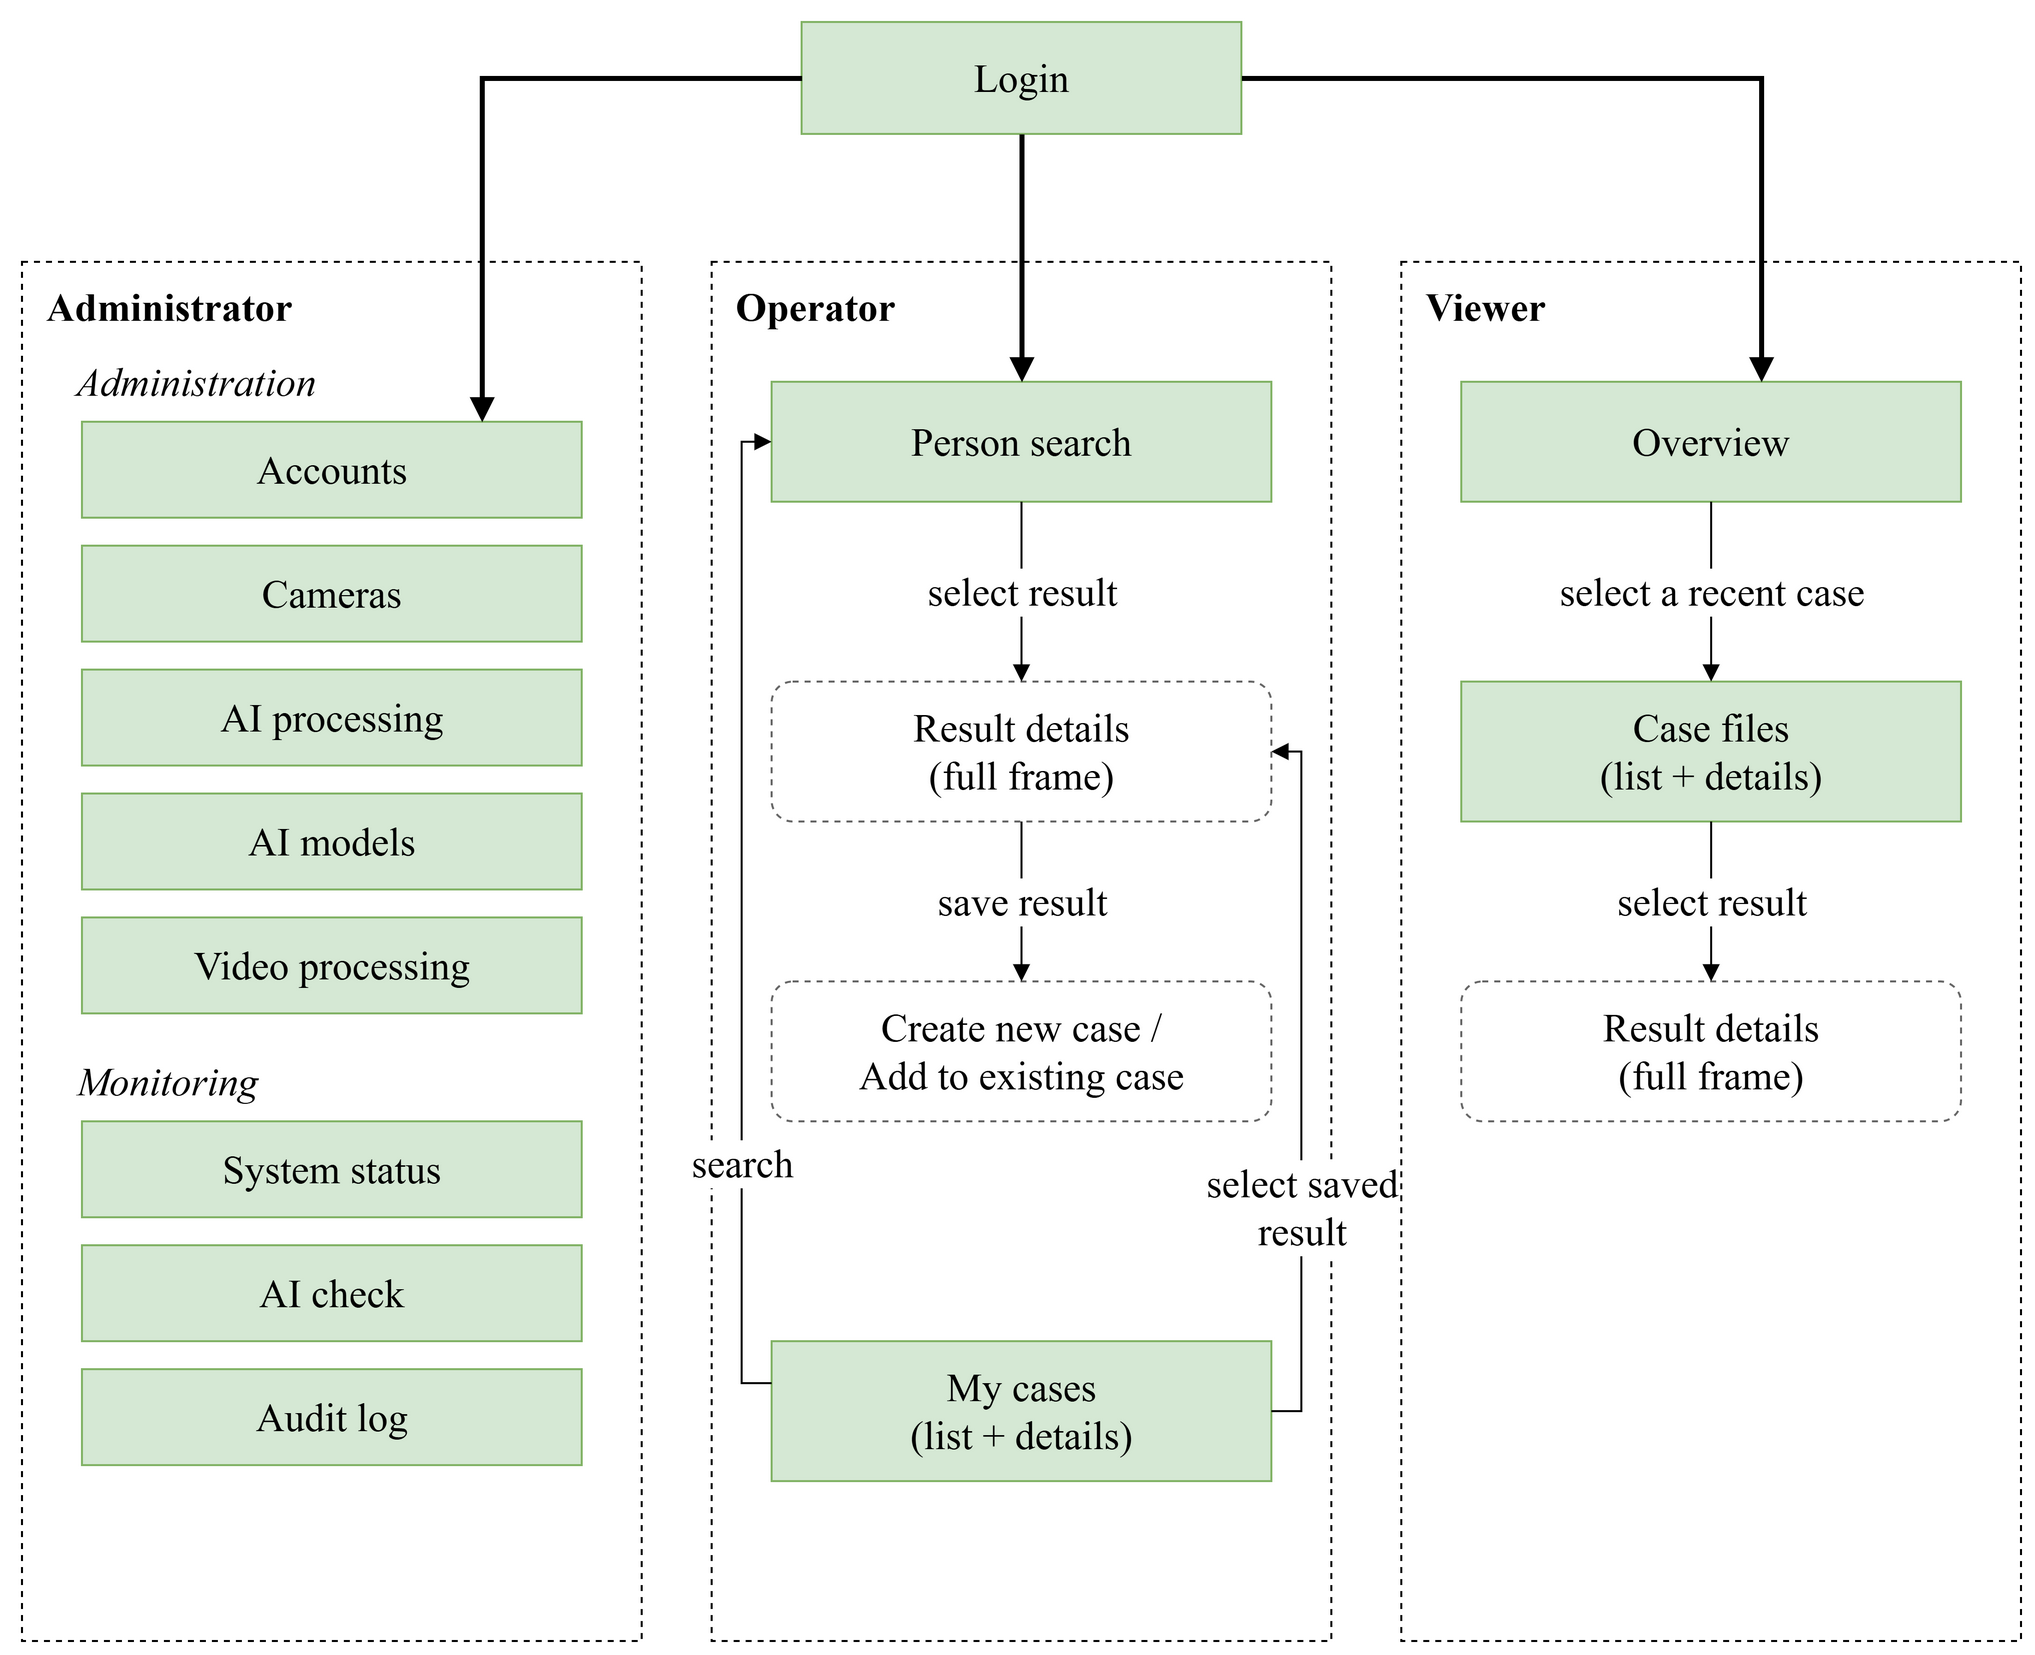
\includegraphics[width=\textwidth]{H12-luong-man-hinh.png}
\caption{Screen flow by role}
\label{fig:screen-flow}
\end{figure}

\begin{itemize}
    \item \textbf{The Administrator} has eight screens in an \emph{Administration} and a \emph{Monitoring} group.
    \item \textbf{The Operator} works mainly on \emph{Person search}, where the query form and results share one page so searches can be repeated; a result opens a detail dialog from which it is saved into a case. \emph{My cases} shows the list and details of cases on one page.
    \item \textbf{The Viewer} starts from \emph{Overview} and opens cases in \emph{Case files}, a read-only version of the Operator's case screen.
\end{itemize}

\subsection{Design Principles}
\label{sec:5.6.2}

Since every result needs the user's confirmation, the interface first supports visual assessment (NFR-20): person images are shown in their frame, with the person highlighted when there are several, and rank, camera and time come first while the score is secondary.

It also saves repetitive actions: query images can be given in several ways, including dragging a result back into the search box (FR-O01), and results can be sorted and filtered without a new query.

Empty results come with a reason and a suggestion, errors use the server's Vietnamese messages, and conflicting changes ask the user to reload. On a phone about 390 pixels wide, the menu becomes a drop-down list and wide tables scroll horizontally.


% !TEX root = ../../main.tex
% Chapter 6 (Part I) - translated from the Vietnamese edition.
\chapter{System Implementation}
\label{chapter:hienthuc}

\textit{This chapter presents the evaluation and choice of technologies and models, the implementation of the background AI worker and of the user interface, and the operation monitoring tools.}

% !TEX root = ../../main.tex
% C6.1 - Choice of technologies and models (translated). YOLO11 figures from docs.ultralytics.com/models/yolo11.
\section{Evaluation and Choice of Technologies and Models}
\label{sec:6.1}

The options were evaluated against four common criteria: meeting the requirements of Chapter~\ref{chapter:phantich}; running on a CPU-only machine with 16~GB of memory; being open-source software with a licence suited to a non-commercial project; and the developer's familiarity with them, to reduce risk within limited time. Table~\ref{tab:tech-summary} summarises the choices, and the subsections below explain the important ones.

\begin{table}[H]
\centering
\caption{Summary of technology and model choices}
\label{tab:tech-summary}
\begin{tabularx}{\textwidth}{|>{\raggedright\arraybackslash}p{3.0cm}|>{\raggedright\arraybackslash}p{3.1cm}|>{\raggedright\arraybackslash}p{3.4cm}|L|}
\hline
\textbf{Component} & \textbf{Choice} & \textbf{Alternatives considered} & \textbf{Main reason} \\
\hline
Front end & React 19, Vite, Tailwind CSS & Server-side rendering; Angular, Vue & Many interactions on one screen; front end and server separated by an API \\
\hline
Server & Python, Flask 3.1, SQLAlchemy, Alembic & Django, FastAPI & Same language as the AI models; small and explicit \\
\hline
Queue & A table in PostgreSQL & Celery with Redis or RabbitMQ & One sequential worker; few infrastructure components \\
\hline
Relational database & PostgreSQL 17 & MySQL & CHECK constraints, partial indexes, JSONB, \texttt{SKIP LOCKED} \\
\hline
Vector storage & Milvus 2.6 & pgvector, FAISS & Pre-filtering, durable storage, one collection per version \\
\hline
Frame storage & MinIO & Files on disk & Bucket-level permissions, hashes, shared with Milvus \\
\hline
Person detection & YOLO11n & YOLO11s, YOLO11m, YOLOX, Faster R-CNN & Fastest on CPU; YOLOX as a licence fallback \\
\hline
Tracking & ByteTrack (default), BoT-SORT & DeepSORT, StrongSORT & No appearance features per person per frame \\
\hline
Encoder & RaSa & Two separate models; CLIP & One shared space for the three forms of query \\
\hline
\end{tabularx}
\end{table}

\subsection{Front-End Technologies}
\label{sec:6.1.1}

The interface has many interactions on one screen, such as dragging and pasting a query image, sorting and filtering results without a new query, and opening dialogs over the list. These interactions suit a \emph{single-page application}, in which the browser loads the application once and then only exchanges data through the API, better than server-side rendering. React was chosen for its large ecosystem with ready-made libraries for routing, API calls and styling, together with Vite for development and bundling, and Tailwind CSS to keep the layout consistent and responsive on phones.

\subsection{Server-Side Technologies}
\label{sec:6.1.2}

The server and the background worker are written in Python because all the project's AI models are provided for Python. Using one language lets the server load the query encoder directly and share the data access code with the background worker. Among the three common frameworks, Django is heavier than an API-only server needs, and the asynchronous advantage of FastAPI matters little because the slowest task, video analysis, has already been moved out of the server (Section~\ref{sec:5.1.3}). Flask is small and explicit, and the developer had already used it. The queue lives in PostgreSQL instead of Celery with Redis or RabbitMQ, because there is only one sequential worker, while each additional infrastructure component costs memory on the target machine.

\subsection{Database and Storage}
\label{sec:6.1.3}

PostgreSQL was chosen because it supports the features the design uses directly: complex CHECK constraints, partial indexes, the JSONB type for logs and measurements, and row locking that skips locked rows (\texttt{SKIP LOCKED}) for safe job claiming. For vector storage, pgvector~\cite{pgvector2026} was suggested at first because it only needs one database, but with an approximate index the filter is applied \emph{after} the index scan, so a query may return fewer results than requested (Section~\ref{sec:3.6.3}). FAISS is only an in-memory library, so the application would have to handle storage, filtering and concurrent access itself. Milvus~\cite{wang2021milvus} was chosen because it filters before searching~\cite{milvus2026filtered}, directly meeting the area-based access control requirement; the trade-off is that Milvus needs etcd and an object store, which makes deployment more complex, although in practice all the services in Docker only use about 515~MiB of memory (Section~\ref{sec:8.7}). Frames are stored in MinIO rather than as files on disk to control access per bucket and keep a hash per object. Milvus already needs an object store, so the application shares that MinIO server in a separate bucket.

\subsection{AI Models}
\label{sec:6.1.4}

\paragraph{Person detection.} Two-stage detectors such as Faster R-CNN are too slow on a CPU, so the project chose the YOLO family. Within YOLO11, the model size directly determines the speed on a CPU (Table~\ref{tab:yolo11-sizes}); even with YOLO11n, the pipeline is about seven times slower than real time (Section~\ref{sec:7.2}), so the project chose the smallest size and compensates for accuracy with a low confidence threshold combined with tracking. YOLO11 is licensed under AGPL-3.0, which suits a non-commercial project, but a commercial product would need a commercial licence; YOLOX~\cite{ge2021yolox}, licensed under Apache-2.0, is therefore registered as a fallback.

\begin{table}[H]
\centering
\caption{Comparison of YOLO11 sizes on the COCO validation set~\cite{ultralytics2024yolo11docs}}
\label{tab:yolo11-sizes}
\begin{tabularx}{\textwidth}{|L|>{\raggedright\arraybackslash}p{2.6cm}|>{\raggedright\arraybackslash}p{3.8cm}|>{\raggedright\arraybackslash}p{3.0cm}|}
\hline
\textbf{Model} & \textbf{mAP$_{50\text{--}95}$} & \textbf{CPU time (ms/image)} & \textbf{Parameters (millions)} \\
\hline
YOLO11n & 39.5 & 56.1 & 2.6 \\
\hline
YOLO11s & 47.0 & 90.0 & 9.4 \\
\hline
YOLO11m & 51.5 & 183.2 & 20.1 \\
\hline
\end{tabularx}
\end{table}

\paragraph{Tracking.} Algorithms that add appearance features, such as DeepSORT~\cite{wojke2017deepsort} and StrongSORT~\cite{du2023strongsort}, keep tracks better through long occlusions, but must run an extra model for every person in every frame, a heavy burden on a CPU in crowded scenes. With static cameras, the project chose ByteTrack~\cite{zhang2022bytetrack} as the default and integrated BoT-SORT~\cite{aharon2022botsort} as an alternative with ReID and camera motion compensation disabled.

\paragraph{Encoder.} Using two separate models for image and text queries would require storing two vectors per appearance and running two models during indexing. General image-text models such as CLIP~\cite{radford2021clip}, including the multilingual variants considered to support Vietnamese, are weaker at separating small differences in clothing. The project chose RaSa~\cite{bai2023rasa} on the supervisor's recommendation: a single model serves all three forms of query with one vector per appearance (Section~\ref{sec:3.5.4}). Its limitation is that queries are English only. The evaluation on the project's data is presented in Section~\ref{sec:8.4}. Part~II of this report studies a different choice for text queries, CLIP ViT-H/14 followed by a reasoning layer, outside the application (Chapter~\ref{chapter:r-overview}).

% !TEX root = ../../main.tex
% C6.2 - Background AI worker implementation (translated). Matches ai/registry.py, ai/configuration.py, workers/*, services/diagnostics.py.
\section{Background AI Worker Implementation}
\label{sec:6.2}

Section~\ref{sec:5.2.1} presented the processing steps and life cycle of a job. This section presents how the background worker is implemented to run reliably on a CPU-only machine.

\subsection{Model Management and Packaging}
\label{sec:6.2.1}

The system only loads the models declared in a \emph{model registry}, where each entry records an identifier, version, weight file with its SHA-256 hash, preprocessing version and provenance, including the licence; Trackers also list the compatible Detectors. A model can only be used when its weight file exists, the hash matches, the licence has been approved and the model has been trial-loaded successfully; models failing these conditions are still listed on the \emph{AI models} screen with the label \emph{Unavailable}. Currently YOLO11n, ByteTrack, BoT-SORT and RaSa are usable, while the larger YOLO sizes and YOLOX have no weight files yet (Section~\ref{sec:6.1.4}). The hash is recomputed every time a pair of models is selected to run, so a weight file replaced on disk cannot be used silently. When the Administrator applies a new Detector-Tracker configuration, the server trial-loads all three components before saving, and each job uses exactly the configuration version current when it was created.

Each kind of model is wrapped in an \emph{adapter} with a common interface: open to load the model, process one input, and close to release resources. The adapter checks the output before passing it on: the Detector only keeps the person class and valid boxes; RaSa vectors must have 256 dimensions, contain no invalid values and be normalised. As a result, adding a new model, for example enabling YOLOX, only needs the weight file and a registry entry, plus an adapter if the model is of a new kind.

\subsection{Resource Limits and Error Handling}
\label{sec:6.2.2}

Since the target machine has limited memory, the background worker is limited at several levels. The number of threads of the numerical libraries is set to 2, so that the models do not take every CPU core that the application server and the data stores also need. The Detector and the image encoder run in a separate child process; if an inference does not return within 120 seconds, the child process is killed, because a call hanging inside a native library cannot be interrupted from within the same process. Each job runs in its own process with a default total deadline of 3,600 seconds; when the job ends, the process ends with it, so the memory of the models and frames is fully reclaimed by the operating system. Frames are processed one at a time and released immediately, except for the representative frame candidates, which are already bounded.

Each error is tied to the step that caused it and a specific error code, stored with the job for display on the administration screens, and classified in advance as \emph{transient} or \emph{unrecoverable}. For video files, transient errors are retried after 5 seconds, doubling each time up to 300 seconds, at most three times. RTSP sessions are not retried, since that part of the video has passed; the scheduler creates a new session after 5 minutes (Section~\ref{sec:5.2.1}). When the process receives a stop signal, the running job is left \emph{Running} so that it can be claimed again when its lease expires, instead of being marked failed immediately. A global lock in PostgreSQL guarantees that only one process executes jobs at a time, even if the background worker is accidentally started twice.

\paragraph{AI check.}\label{sec:6.2.5} The \emph{AI check} screen trial-runs the models on real data without creating a job: for a camera, the system reads at most 90 frames from the RTSP stream, takes 6 of them and runs the Detector, Tracker and image encoder in turn; for the search group, the system encodes a sample image and a sample description. Each check is limited to 180 seconds, and only one check runs at a time.

% !TEX root = ../../main.tex
% C6.3 - User interface implementation (translated). The screenshots show the application's Vietnamese interface;
% screen and label names in the text are their English meaning.
\section{User Interface Implementation}
\label{sec:6.3}

\subsection{Navigation and Communication with the Server}
\label{sec:6.3.1}
\label{sec:6.3.2}

Navigation uses React Router with routes grouped by role: a user without a session goes to the login screen, and a route of another role redirects to the user's own home page. This guard only hides unusable screens; permissions are checked by the server (NFR-01).

All requests go through one API layer. It attaches the CSRF token, kept only in page memory, to every data-changing request (Section~\ref{sec:5.5.2}), and turns errors into Vietnamese messages. Server errors also show a \emph{lookup code}, the first eight characters of the request identifier, so that the matching log line can be found (Section~\ref{sec:6.4}). A 401 response clears the login state and returns to the login screen. The session is refreshed only on real user activity, shared across browser tabs, so background requests do not keep it alive.

\subsection{Rendering Person Images in the Results}
\label{sec:6.3.3}

The server renders each person image from the full frame and bounding box (Section~\ref{sec:5.3.3}). For the 3:5 result card, the crop is widened with the real surrounding scene until it fits, never cutting into the person; since it may then include other people, the surroundings are dimmed to 60\% and the person is outlined in an accent colour. The detail dialog shows the full frame with a red box. Images are sent only to users entitled to the result, marked not to be cached, and a missing frame shows an \emph{Image unavailable} icon.

\subsection{Main Screens}
\label{sec:6.3.4}

The figures show the main screens by role on the demonstration data (Section~\ref{sec:7.2}). The interface is in Vietnamese (NFR-19); screen and label names are given by their English meaning.

\paragraph{Operator.} \emph{Person search} (Figure~\ref{fig:ui-search-image}) has the query form on the left (image, cameras of the area, date range, number of results) and the ranked results on the right, each with the person image in context, camera, time and score; the shared area and date appear once above the list. In attribute search (Figure~\ref{fig:ui-search-attr}), the form shows the generated English description, so users see what is actually searched. A result opens the detail dialog (Figure~\ref{fig:ui-result}), from which it is saved into a case (Figure~\ref{fig:ui-create-case}). \emph{My cases} (Figure~\ref{fig:ui-cases}) lists the cases by status with the details of the selected one; a closed case is locked until reopened.

\begin{figure}[!htbp]
\centering
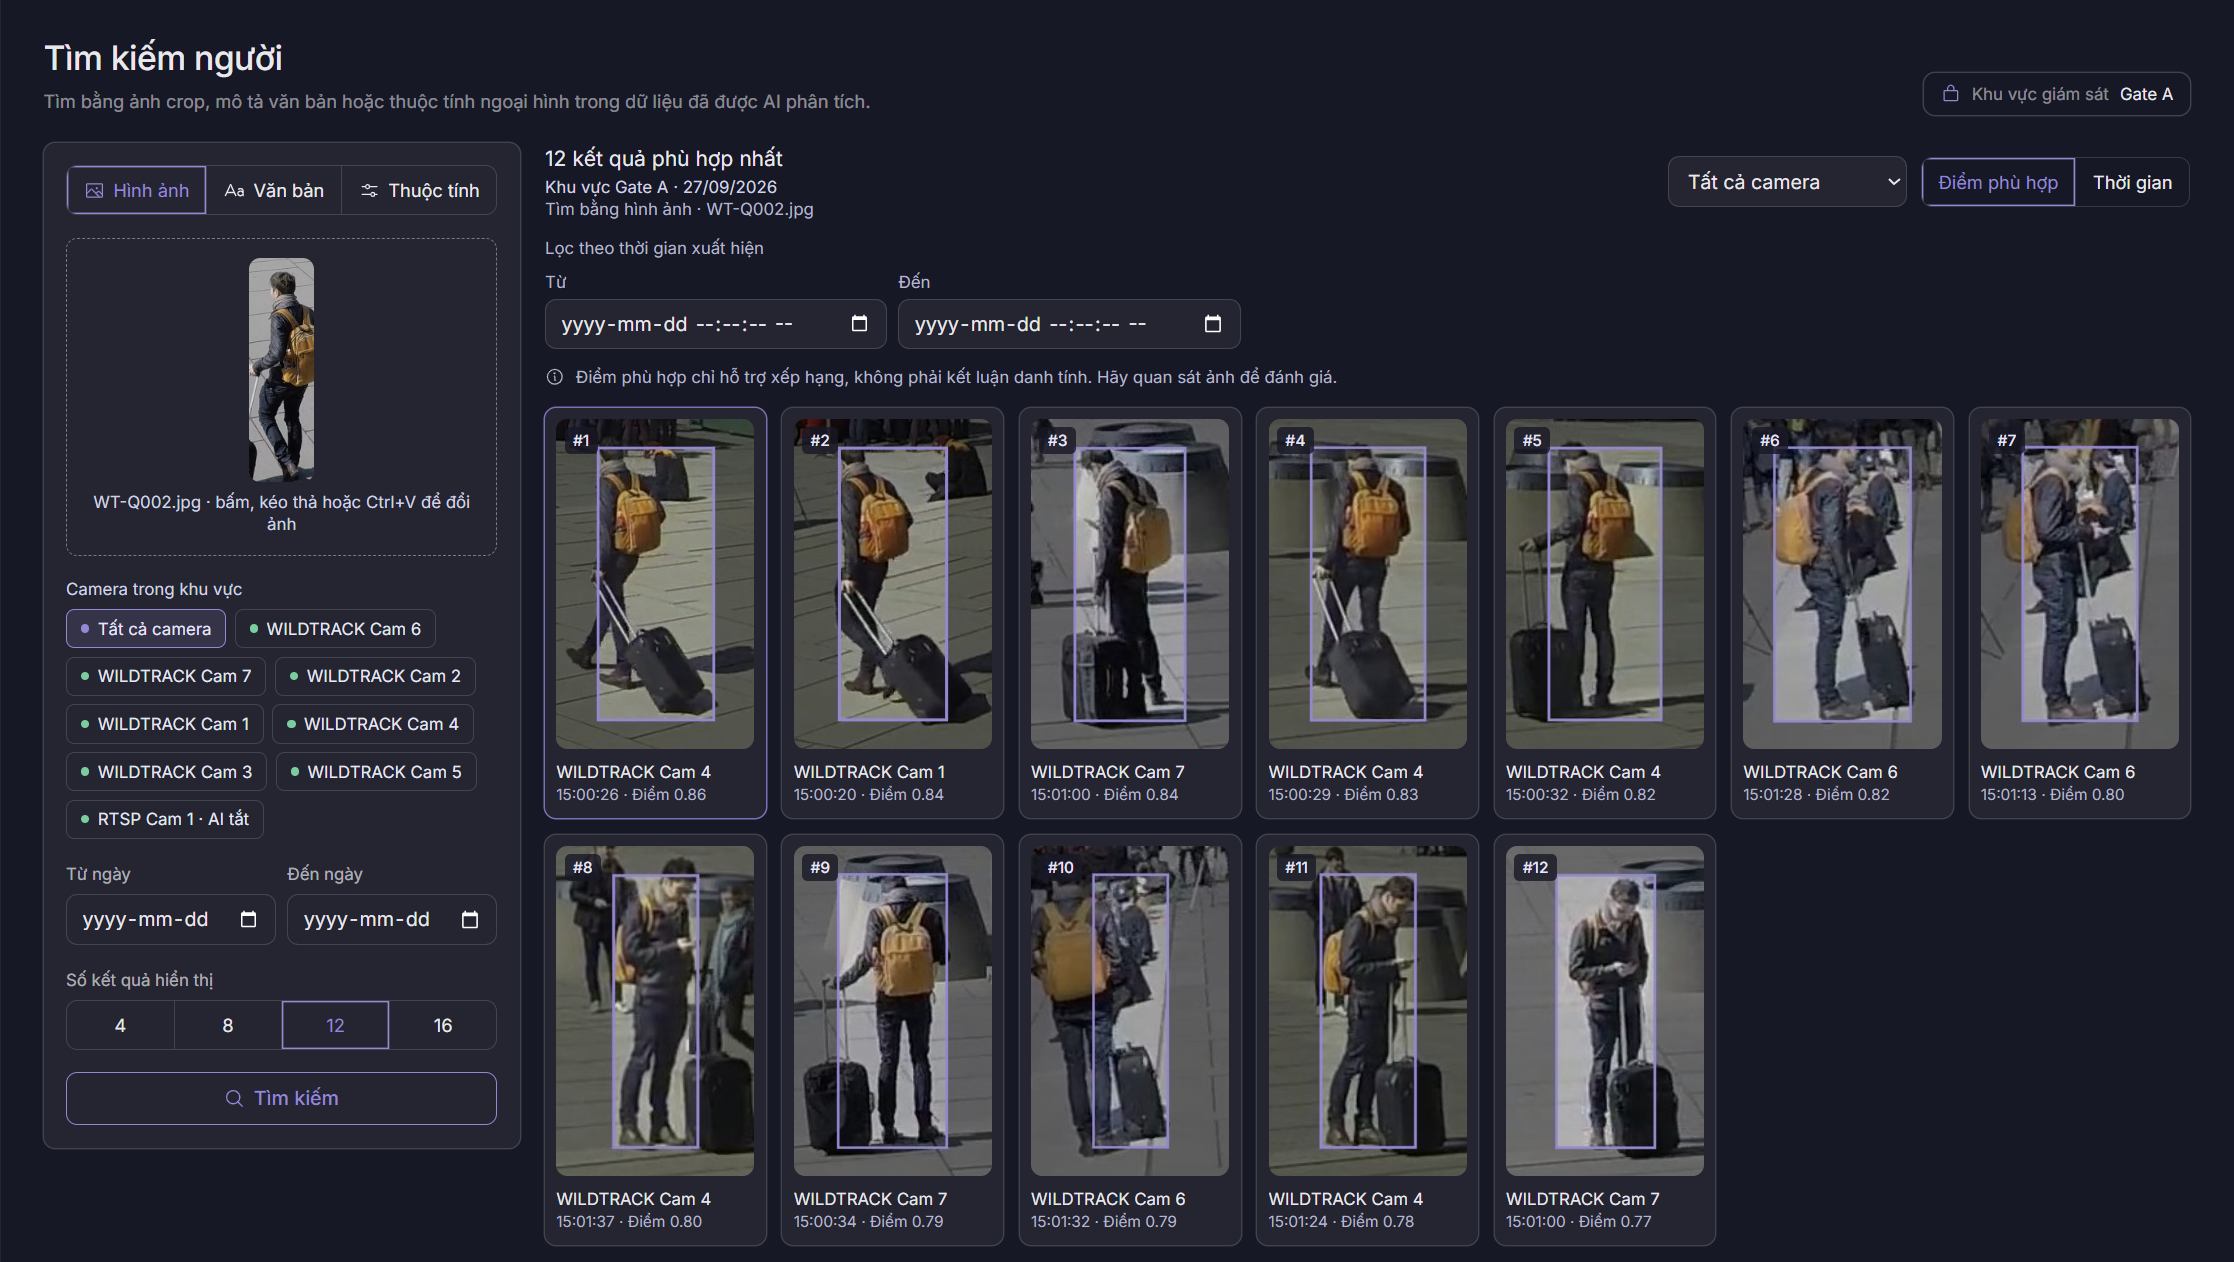
\includegraphics[width=\textwidth]{H10a-tim-kiem-anh-cat.png}
\caption{Person search by image}
\label{fig:ui-search-image}
\end{figure}

\begin{figure}[!htbp]
\centering
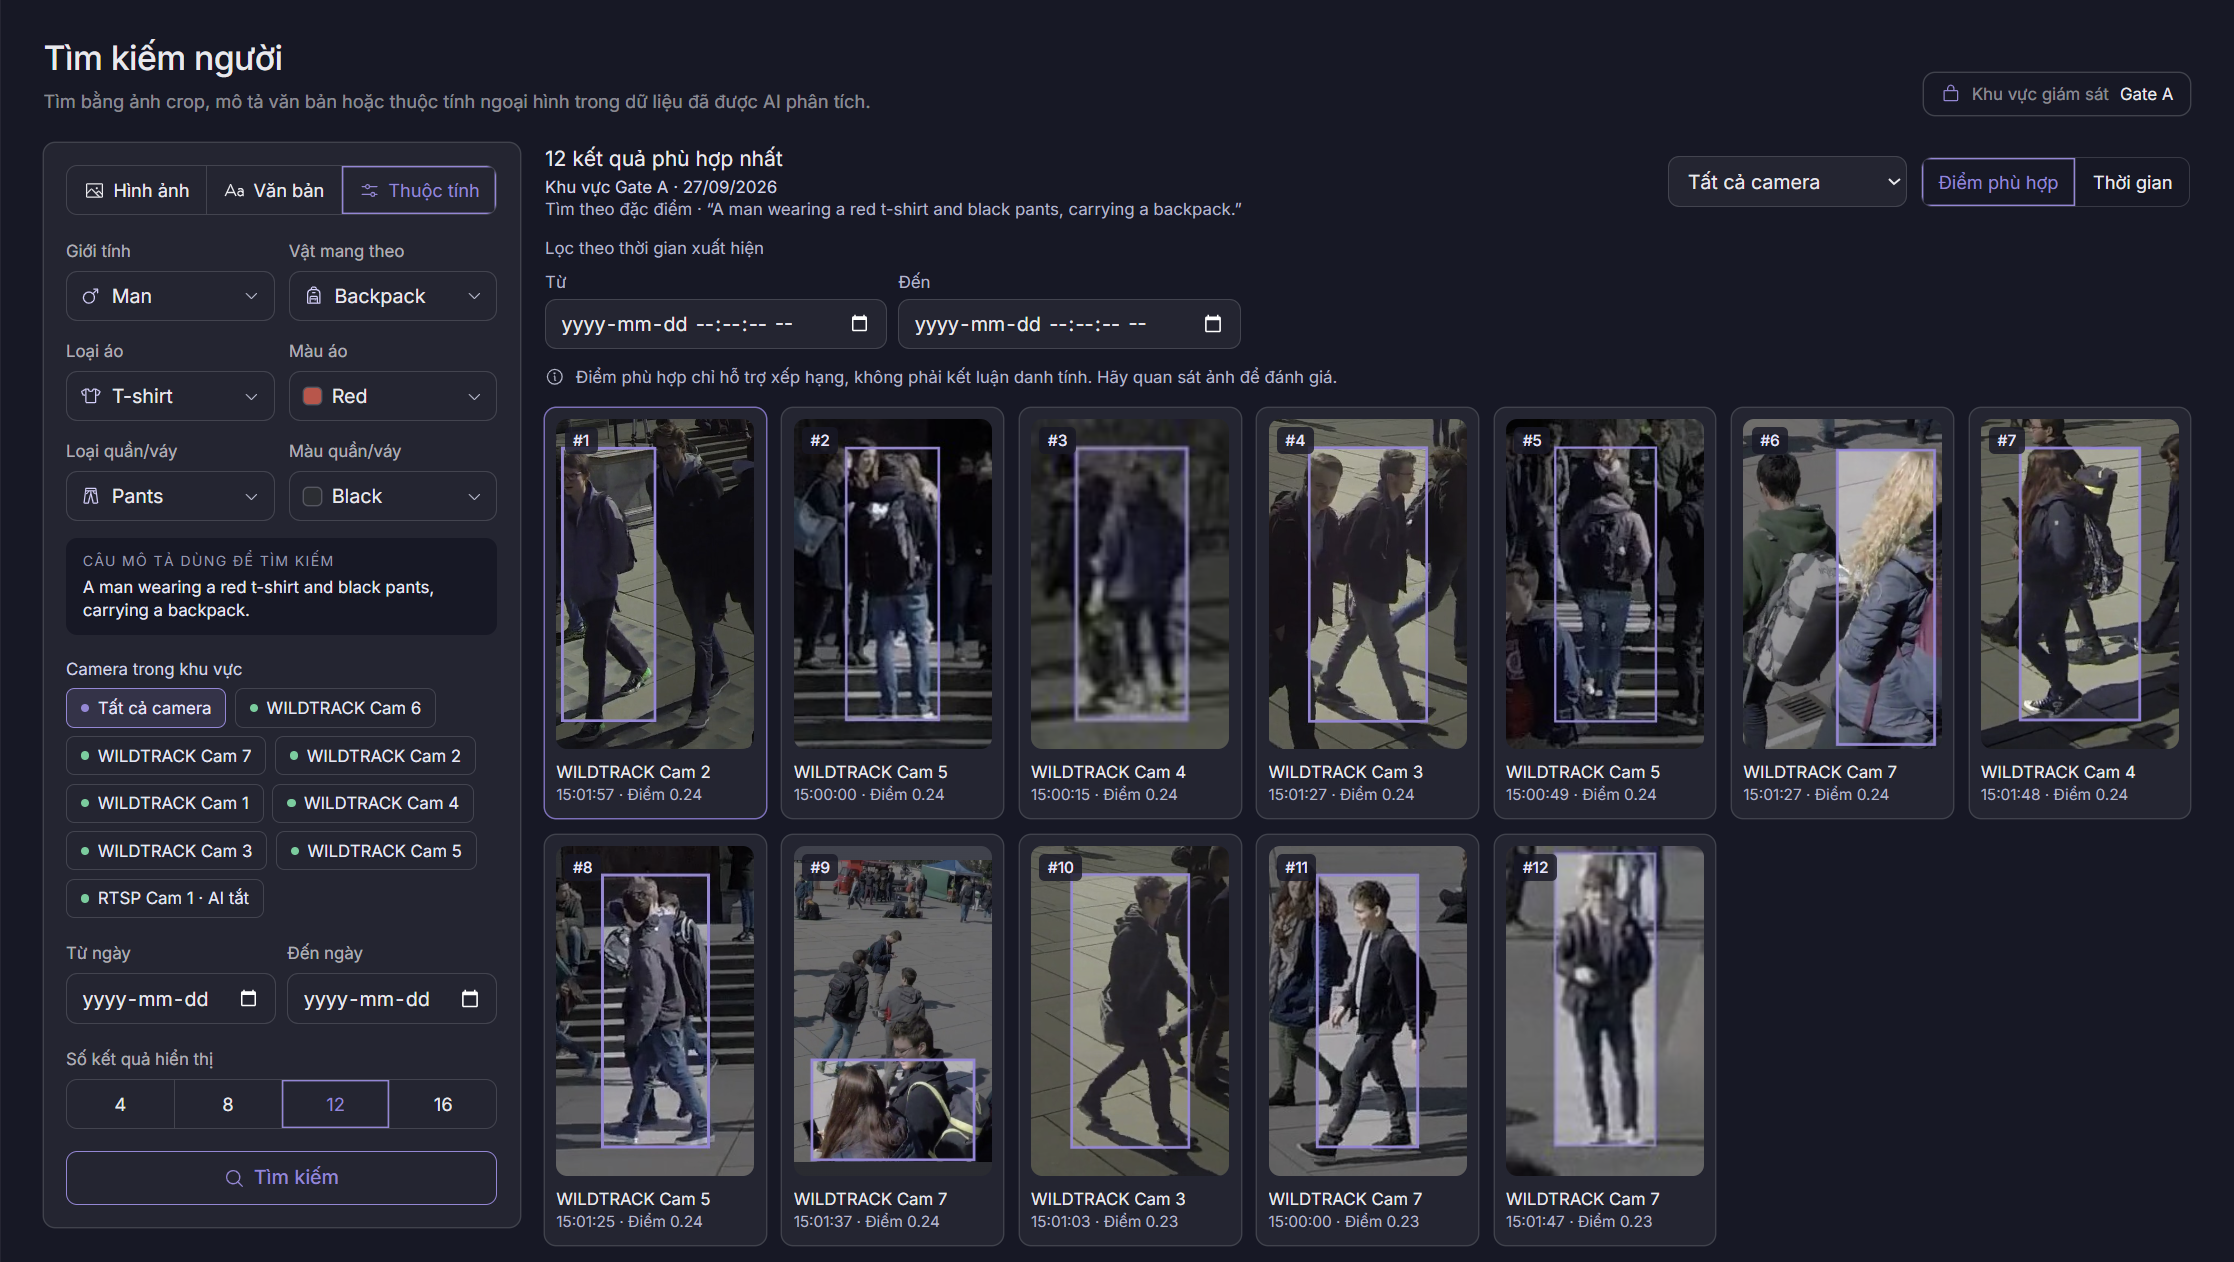
\includegraphics[width=\textwidth]{H10b-tim-kiem-thuoc-tinh-cat.png}
\caption{Person search by attributes}
\label{fig:ui-search-attr}
\end{figure}

\begin{figure}[!htbp]
\centering
\begin{subfigure}[b]{0.61\textwidth}
    \centering
    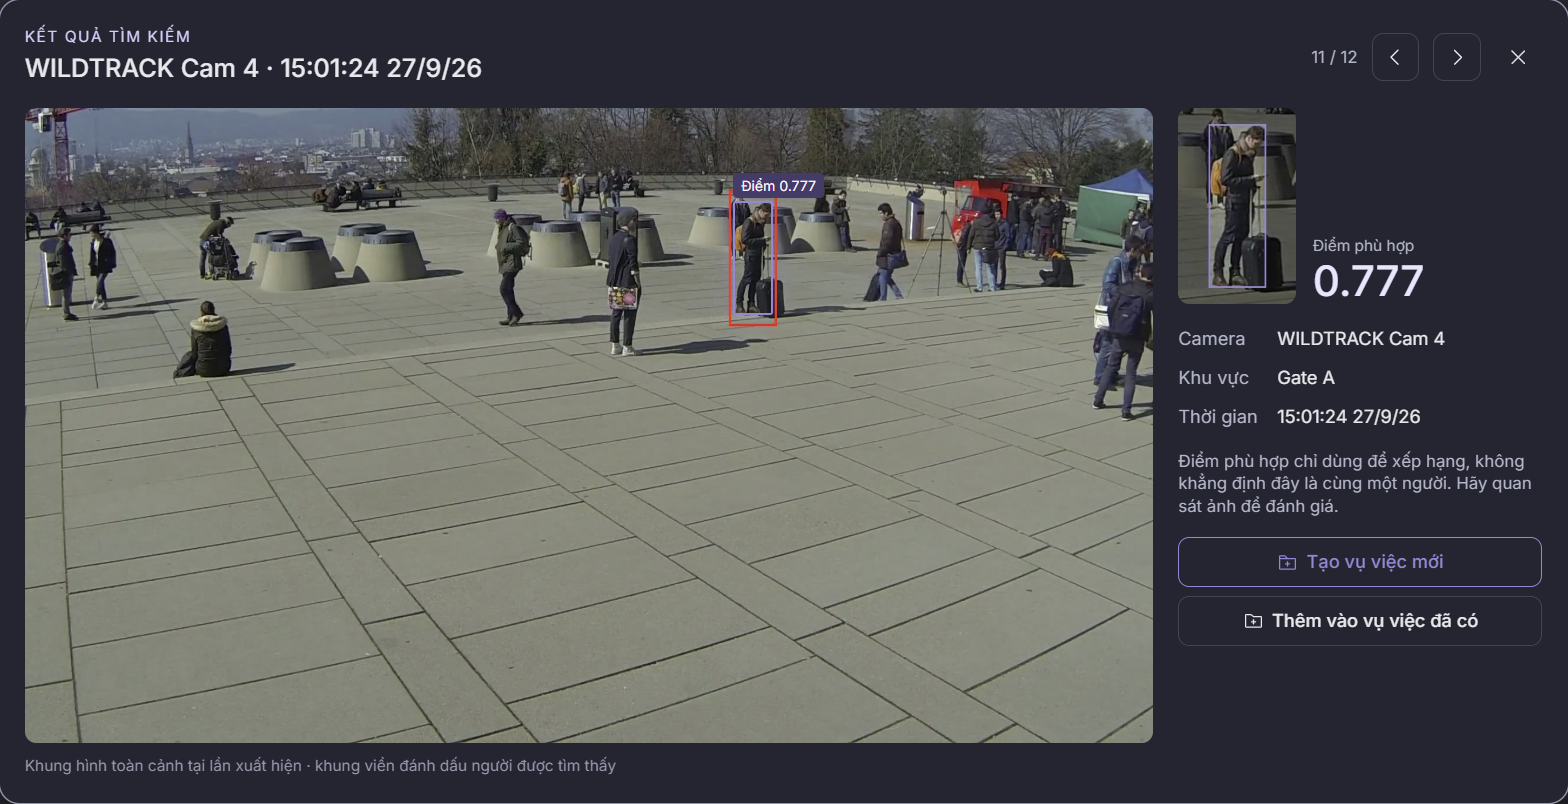
\includegraphics[width=\linewidth]{H10c-chi-tiet-ket-qua-cat.png}
    \caption{Details of a result}
    \label{fig:ui-result}
\end{subfigure}\hfill
\begin{subfigure}[b]{0.36\textwidth}
    \centering
    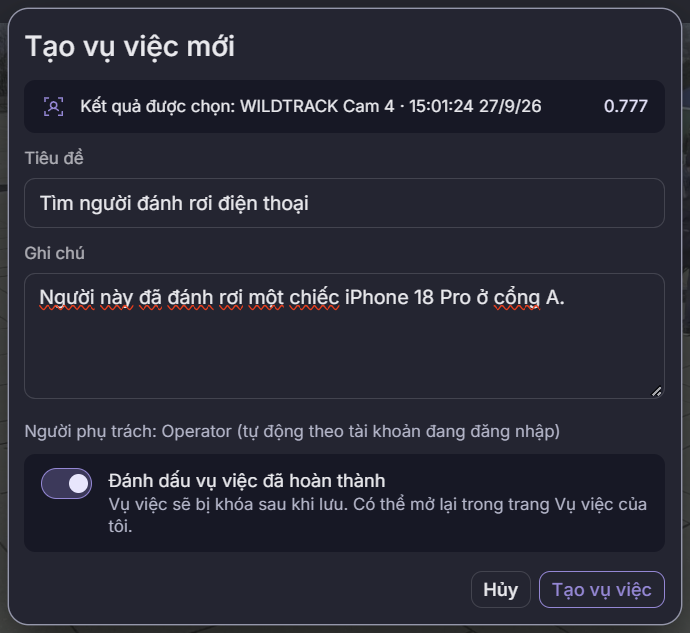
\includegraphics[width=\linewidth]{H10d-tao-vu-viec-cat.png}
    \caption{Creating a case from a result}
    \label{fig:ui-create-case}
\end{subfigure}
\caption{The result detail dialog and the case creation dialog}
\label{fig:ui-result-case}
\end{figure}

\begin{figure}[!htbp]
\centering
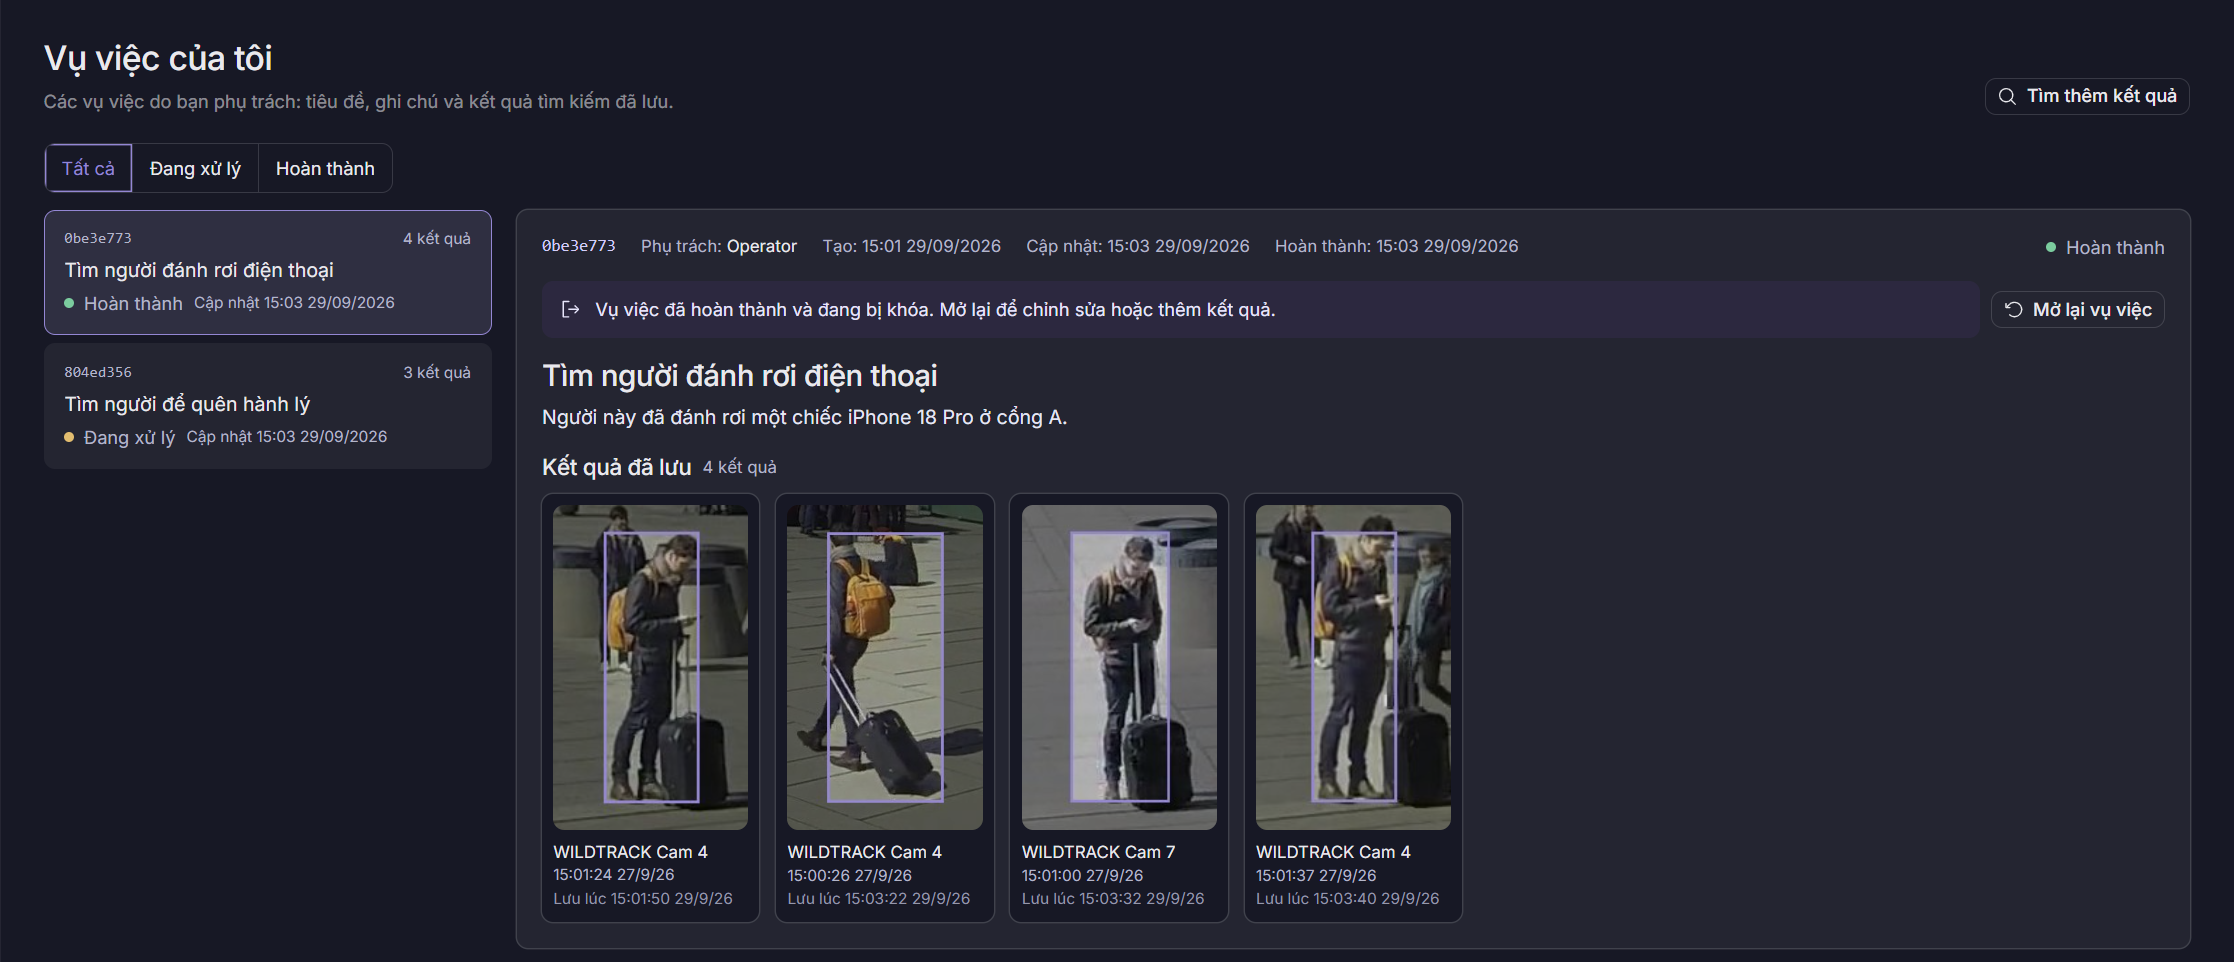
\includegraphics[width=\textwidth]{H10e-vu-viec-cua-toi-cat.png}
\caption{The Operator's case management screen}
\label{fig:ui-cases}
\end{figure}

\paragraph{Viewer.} \emph{Overview} (Figure~\ref{fig:ui-overview}) shows cases by status, saved results and recent cases; a case opens in \emph{Case files}, a read-only version of Figure~\ref{fig:ui-cases}.

\begin{figure}[!htbp]
\centering
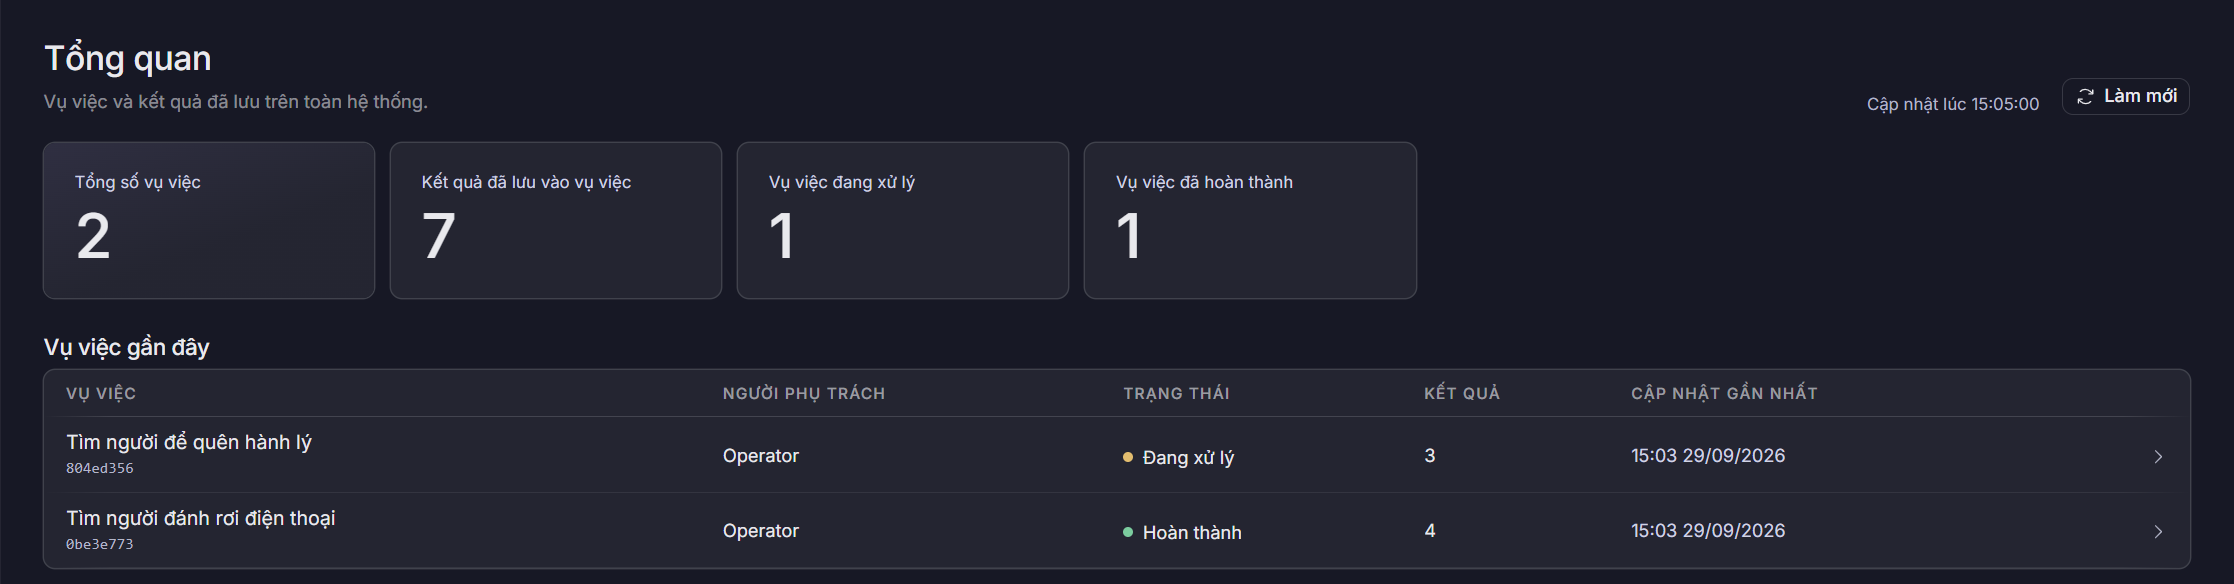
\includegraphics[width=\textwidth]{H10f-tong-quan-cat.png}
\caption{The Viewer's overview screen}
\label{fig:ui-overview}
\end{figure}

\paragraph{Administrator.} \emph{Cameras} (Figure~\ref{fig:ui-cameras}) lists the cameras by area with their connection status (\emph{Uploaded video} for file-only cameras), AI processing status and actions. \emph{AI models} (Figure~\ref{fig:ui-models}) selects the Detector and Tracker, marking unusable models and showing the encoder as fixed (Section~\ref{sec:6.2.1}). \emph{Video processing} (Figure~\ref{fig:ui-video}) uploads a video with a sampling preset and follows each job by frames and ready tracks. The monitoring screens are \emph{System status} (Figure~\ref{fig:ui-status}, Section~\ref{sec:6.4}) and \emph{AI check} (Figure~\ref{fig:ui-diagnostics}, Section~\ref{sec:6.2.5}).

\begin{figure}[!htbp]
\centering
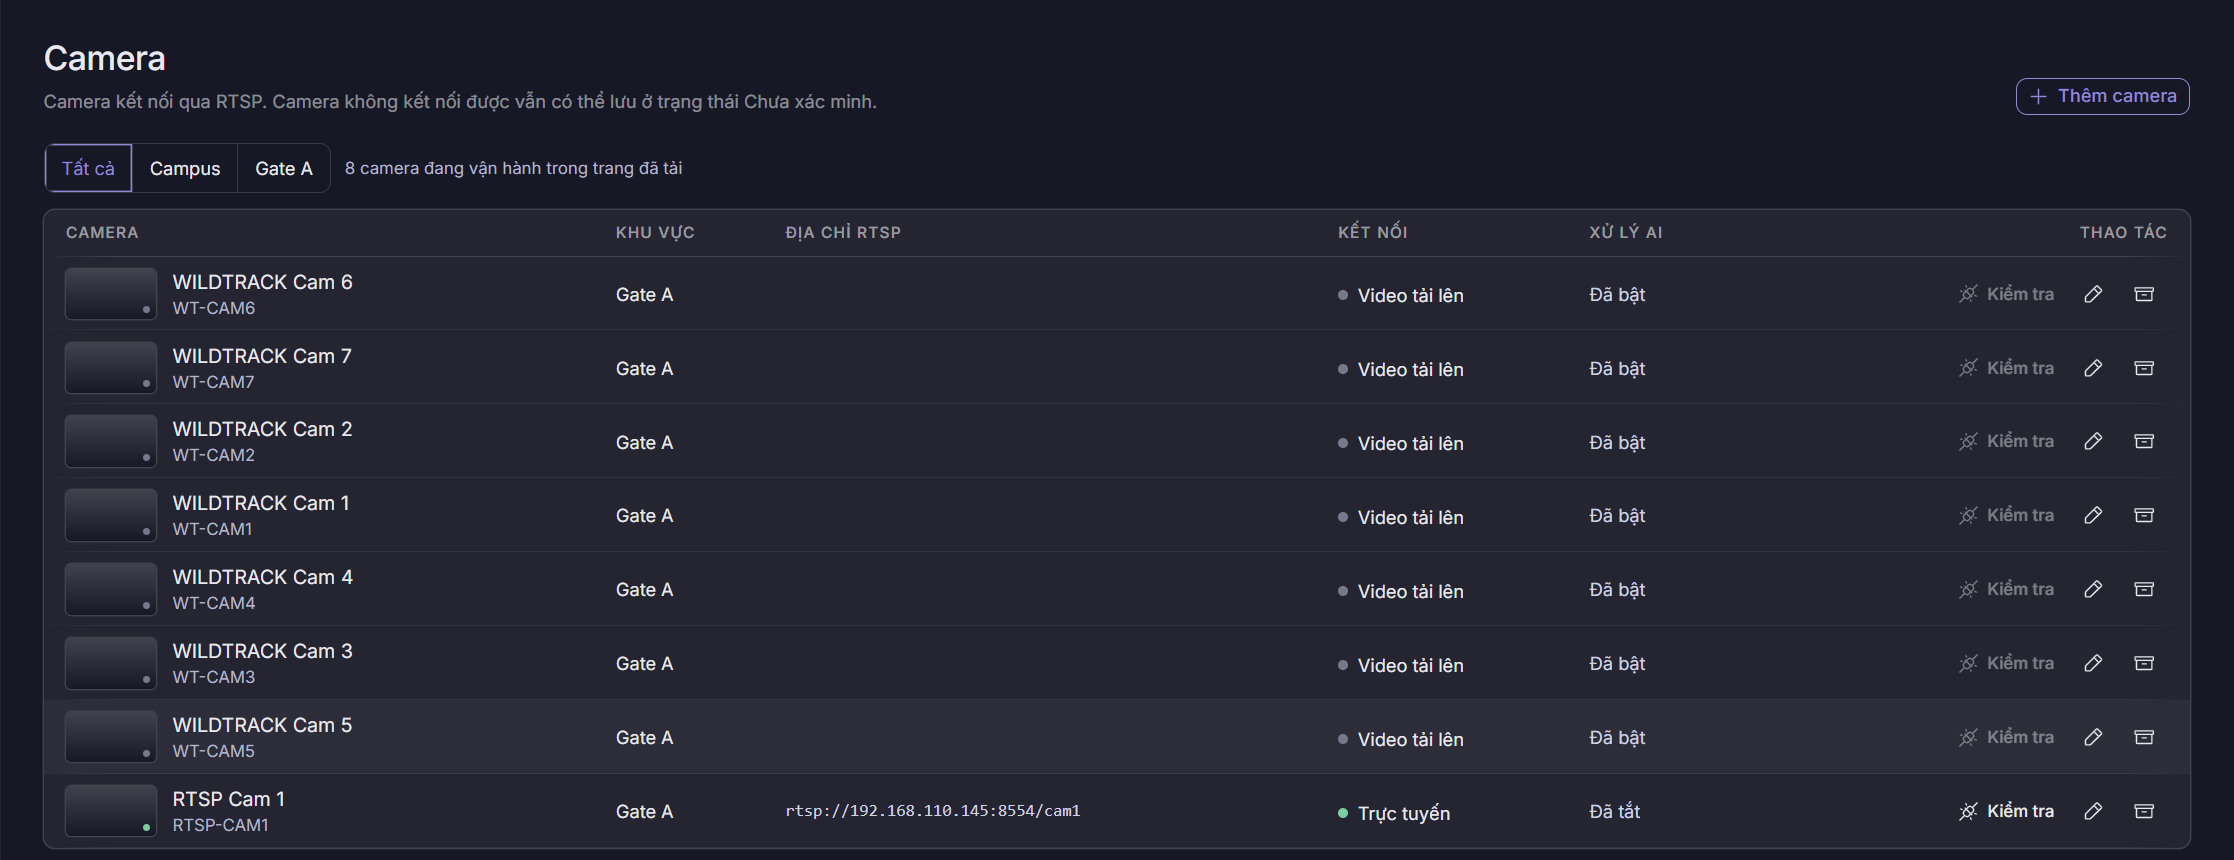
\includegraphics[width=\textwidth]{H10g-camera-cat.png}
\caption{Camera management screen}
\label{fig:ui-cameras}
\end{figure}

\begin{figure}[!htbp]
\centering
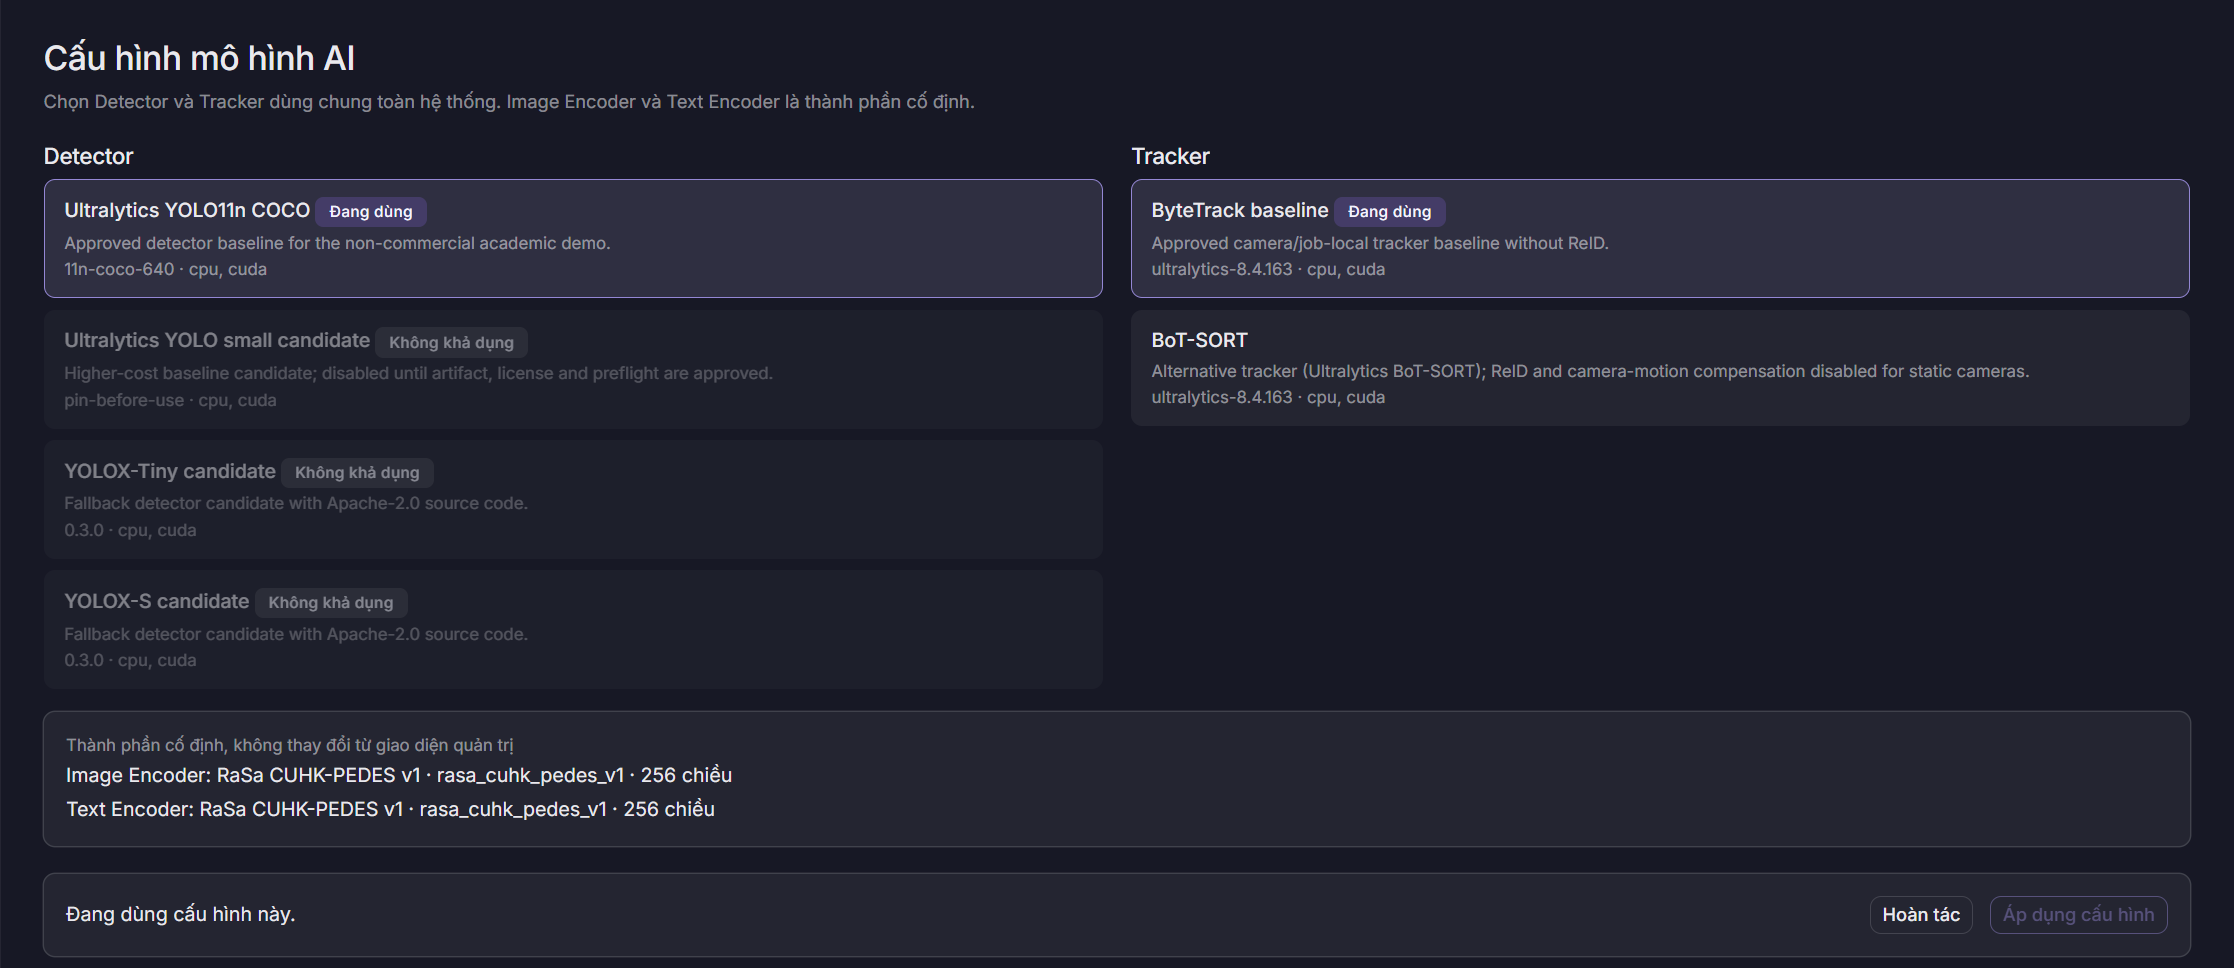
\includegraphics[width=\textwidth]{H10h-mo-hinh-ai-cat.png}
\caption{AI model configuration screen}
\label{fig:ui-models}
\end{figure}

\begin{figure}[!htbp]
\centering
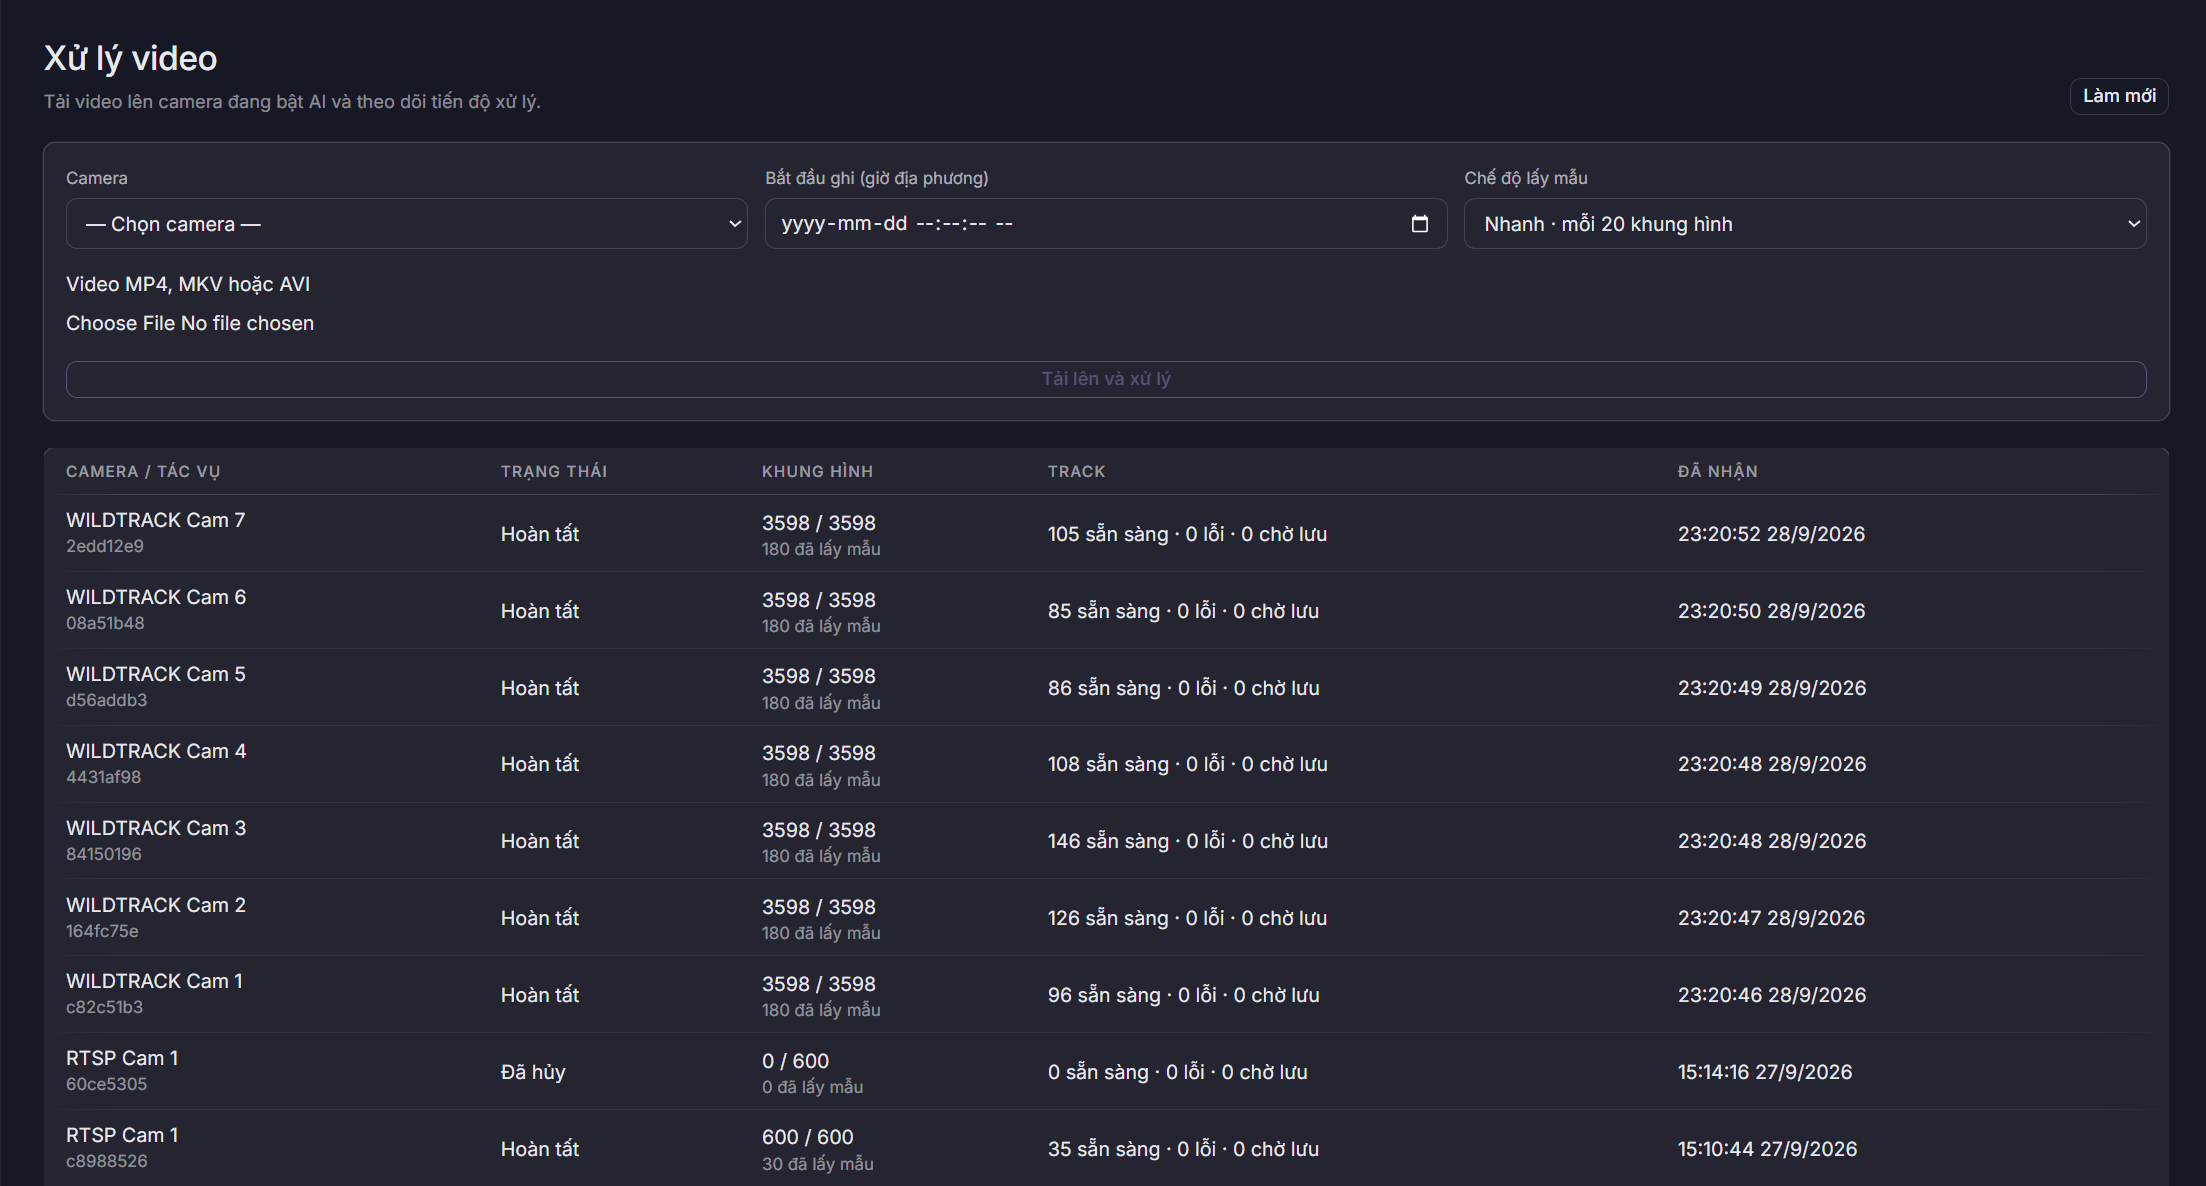
\includegraphics[width=\textwidth]{H10i-xu-ly-video-cat.png}
\caption{Uploaded video processing screen}
\label{fig:ui-video}
\end{figure}

\begin{figure}[!htbp]
\centering
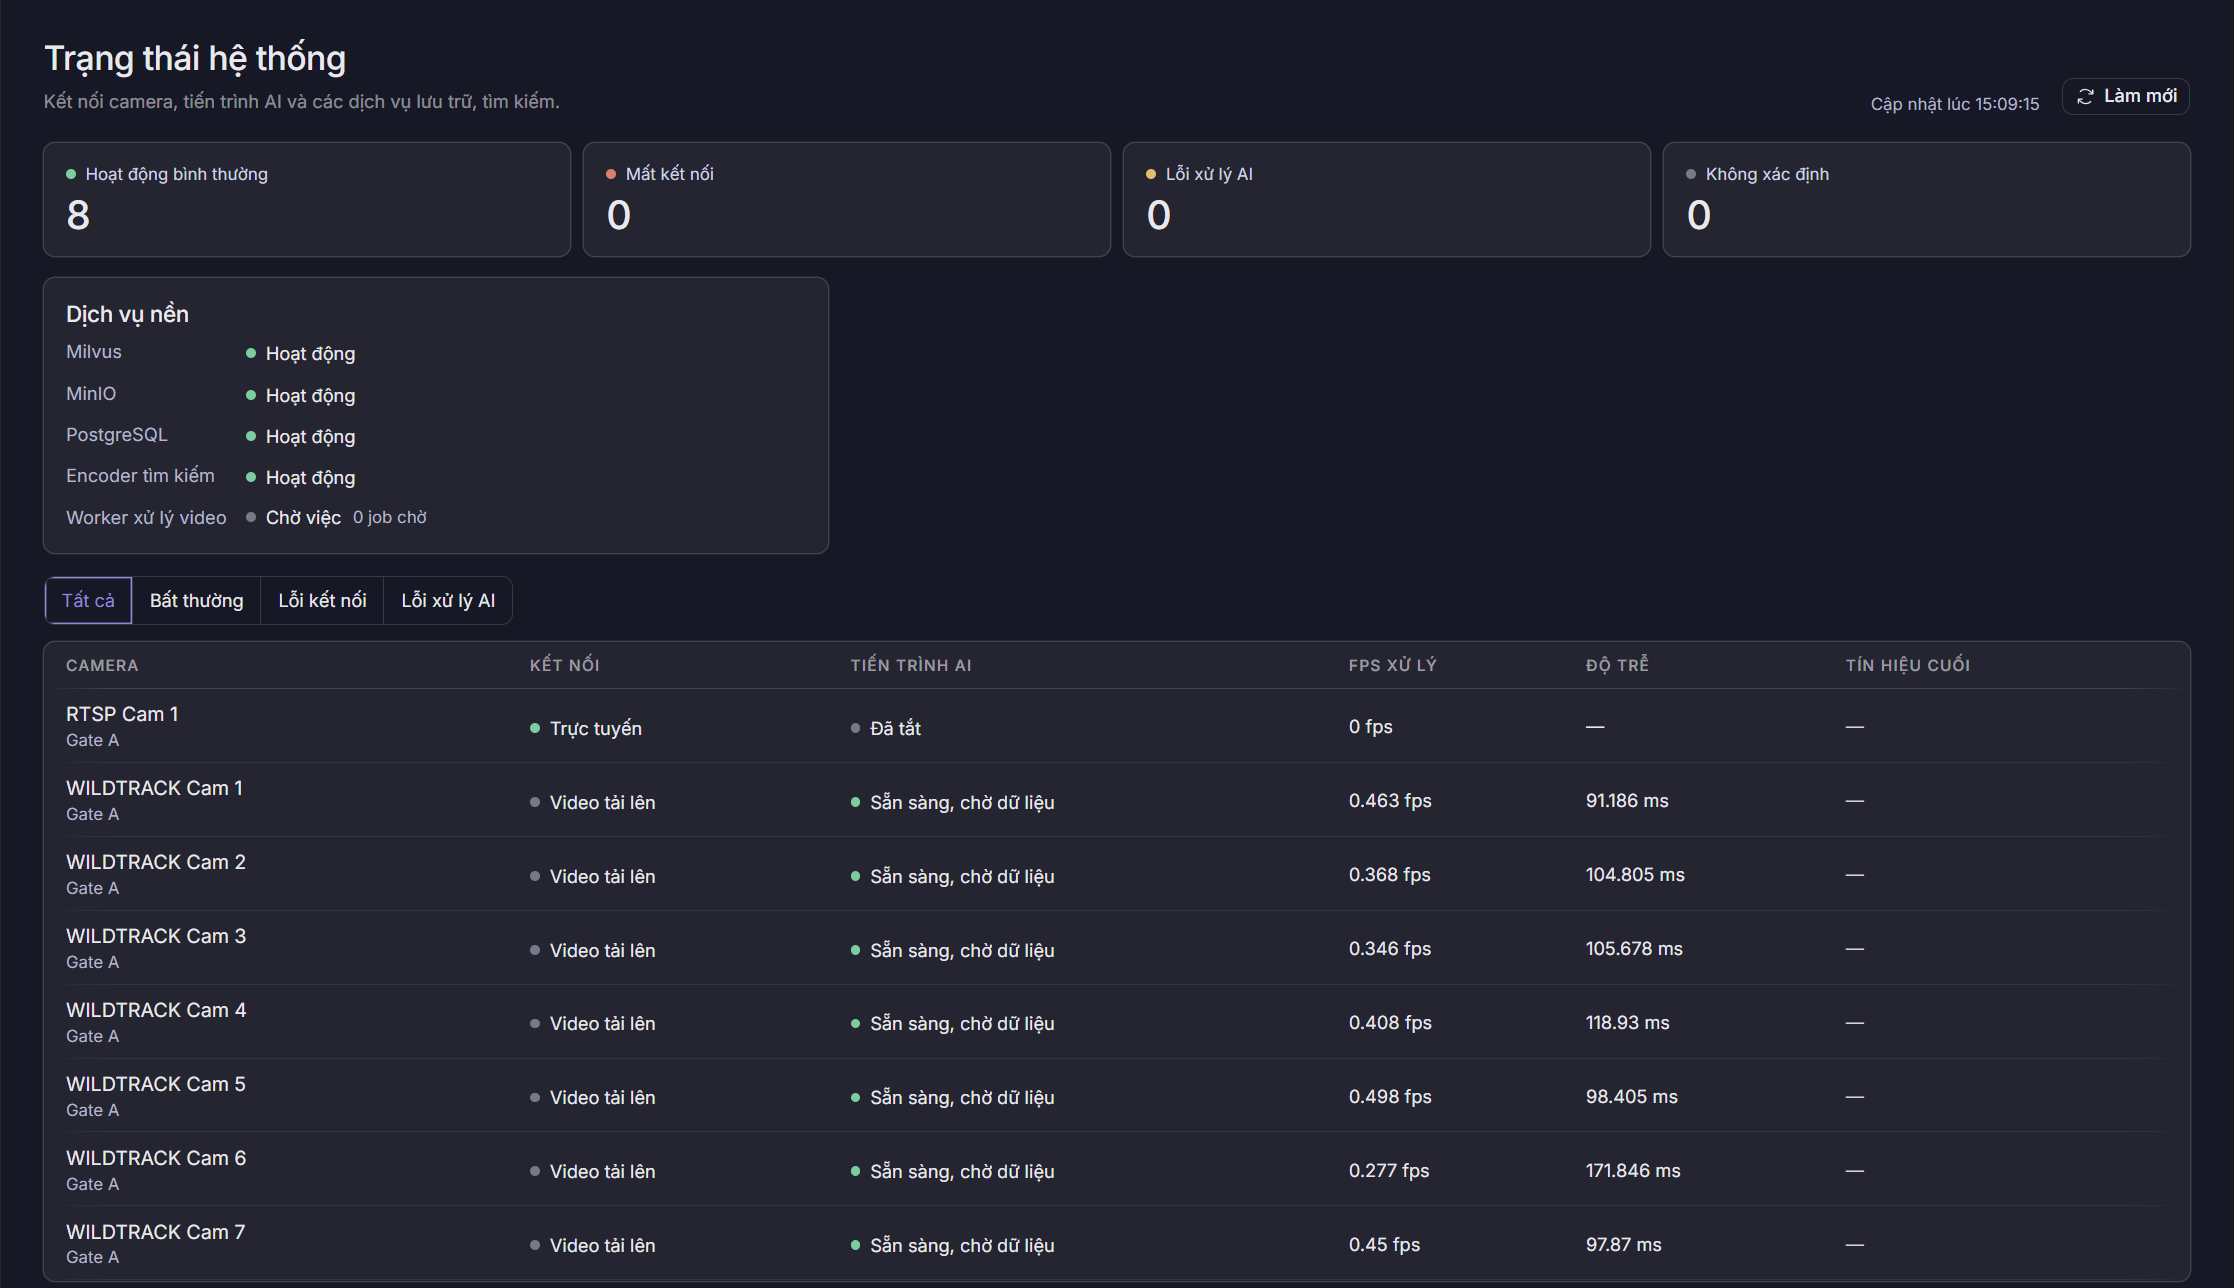
\includegraphics[width=\textwidth]{H10j-trang-thai-he-thong-cat.png}
\caption{System status screen}
\label{fig:ui-status}
\end{figure}

\begin{figure}[!htbp]
\centering
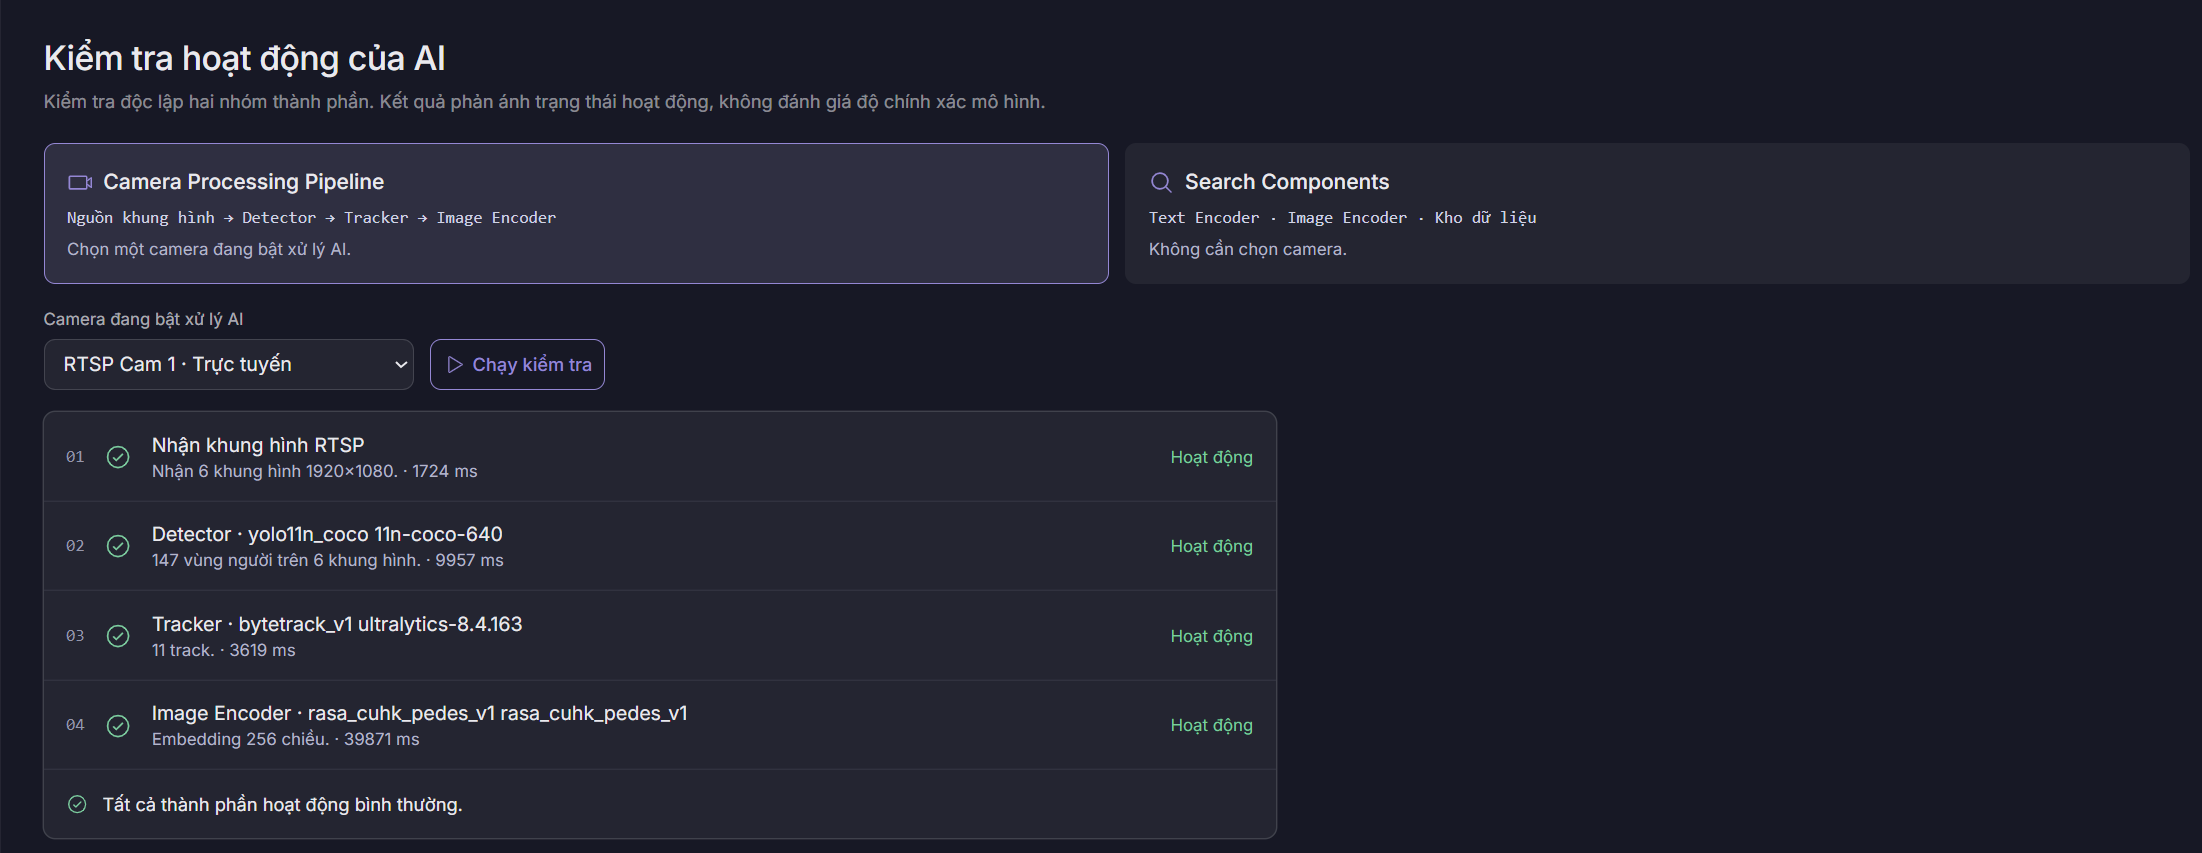
\includegraphics[width=\textwidth]{H10k-kiem-tra-ai-cat.png}
\caption{AI check screen}
\label{fig:ui-diagnostics}
\end{figure}

% !TEX root = ../../main.tex
% C6.4 - Operation monitoring (translated). Matches observability.py, services/audit.py, workers/telemetry.py, services/monitoring.py.
\section{Operation Monitoring}
\label{sec:6.4}

\paragraph{Technical logs.} The server and the worker write JSON logs, one event per line, tagged with the request identifier or with the job, camera and AI configuration identifiers, so the \emph{lookup code} of an error message (Section~\ref{sec:6.3.2}) or a failed job's identifier finds all related lines. Sensitive fields such as passwords, tokens, RTSP addresses, vectors, images and query sentences are replaced by \texttt{[REDACTED]}, and credentials, vector-like number sequences or encrypted data in free text are masked.

\paragraph{Audit log.} Important user actions and operational events are stored in PostgreSQL as 32 event types, from logins and session expiry to account, camera and AI configuration changes, processing and AI check errors, jobs, cases and maintenance tools; the \emph{Audit log} screen filters them by date, type, actor and outcome.

\paragraph{Metrics and system status.} A running job updates its metrics about every 2 seconds (frame rate, average Detector, Tracker and encoder time, memory, CPU), and the worker sends a heartbeat every 10 seconds, being considered down after 45 seconds of silence. \emph{System status} (Figure~\ref{fig:ui-status}) gathers, for each camera, its RTSP and AI status, rate, latency and failed jobs in 24 hours, placing it in one of four groups (normal, offline, AI error, unknown), and for the components, the health of the three stores, the search encoder and the queue. Each value shows its age, so stale numbers are not mistaken for the current state.


% !TEX root = ../../main.tex
% Chapter 7 (Part I) - translated. Figures only from files/report-data-guide.md section 3.
\chapter{System Deployment}
\label{chapter:trienkhai}

\textit{This chapter presents the deployment environment and procedure of the system, together with the test data and the simulation of the camera system.}

% !TEX root = ../../main.tex
% C7.1 - Environment and deployment procedure (translated). Figures: report-data-guide.md section 2 and C7.3 (current).
\section{Environment and Deployment Procedure}
\label{sec:7.1}
\label{sec:7.3}

\paragraph{Environment.} The whole system is deployed on a laptop with an Intel Core i5-11300H processor (4 cores, 8 threads, 3.1~GHz), 16~GB of memory and no discrete graphics card, running Windows 11. The infrastructure services run in Docker Compose: PostgreSQL 17, Milvus 2.6 in Standalone mode with etcd, MinIO shared by Milvus and by the application's frames, and MediaMTX to stream the simulated cameras. The Flask application server, the background worker and the React web application run directly on the machine. The AI configuration is YOLO11n with a confidence threshold of 0.1, ByteTrack, the RaSa encoder and a sampling interval of $N = 20$, all running on the CPU.

\paragraph{Start-up procedure.} The components are started in order: infrastructure services, simulated camera streams, application server, background worker, then the web application. Since the query encoder is only loaded at the first search, a warm-up search is run before use (Section~\ref{sec:8.7}).

\paragraph{Backup and restore.} The backup of the demonstration data of the three stores is about 510~MB in 1,525 files. The restore procedure was rehearsed with 1,555 tracks, 10 of whose frames had been deleted on purpose: the restore finished in 28.8 seconds (PostgreSQL 1.8 seconds; frames 6.2 seconds, with all 10 of 10 files re-uploaded; rebuilding the Milvus vectors 8.8 seconds; reconciling the three stores 12 seconds). The first rehearsal, when vectors were still written one by one, took 1,485 seconds and had one vector time out, which led to the switch to batch writes. After each demonstration rehearsal, the data is reset to its baseline in about 70 seconds.

% !TEX root = ../../main.tex
% C7.2 - Test data and simulated cameras (translated). Figures: report-data-guide.md section 2 and C7.2 (current).
\section{Test Data and Simulated Cameras}
\label{sec:7.2}

\paragraph{Dataset.} The project uses the WILDTRACK dataset~\cite{chavdarova2018wildtrack}, made of the videos of seven static 1920$\times$1080 cameras observing one crowded outdoor pedestrian area with overlapping fields of view, together with person position labels on a set of frames. Each video is treated as one camera, and all seven cameras are assigned to the same surveillance area.

\paragraph{Simulated cameras.} The seven videos are streamed as seven RTSP streams through MediaMTX as in Section~\ref{sec:3.7.3}. On the target machine, however, the analysis is about seven times slower than real time, so the streaming server drops frames and most of the stream content is not analysed. The RTSP streams are therefore used to demonstrate and verify camera ingestion (Section~\ref{sec:8.6}), while the demonstration data is indexed from the video files themselves through the video upload function, which goes through the same pipeline.

\paragraph{Preparing the demonstration data.} Indexing is done by a tool that calls the system's API as an Administrator: it cuts the segment of video to process, uploads it for each camera with the same time origin for all seven cameras, and follows the jobs until they finish. The demonstration data covers the first 120 seconds of each video: the 0-60 second segment produced 736 tracks, and the 60-120 second segment was processed by 7 jobs in 55 minutes, adding 752 tracks without errors. In total there are 1,488 ready tracks, distributed as in Table~\ref{tab:demo-tracks}. Together with 35 tracks from one RTSP processing session, the demonstration data has 1,523 tracks and one sample case with 3 results.

\begin{table}[H]
\centering
\caption{Number of tracks in the demonstration data per camera (first 120 seconds of each video)}
\label{tab:demo-tracks}
\begin{tabularx}{\textwidth}{|L|c|c|c|c|c|c|c|c|}
\hline
\textbf{Camera} & C1 & C2 & C3 & C4 & C5 & C6 & C7 & \textbf{Total} \\
\hline
\textbf{Tracks} & 208 & 254 & 308 & 188 & 182 & 159 & 189 & 1,488 \\
\hline
\end{tabularx}
\end{table}


% !TEX root = ../../main.tex
% Chapter 8 (Part I) - translated. Figures ONLY from files/report-data-guide.md section 3, following its status column.
\chapter{Testing and Evaluation}
\label{chapter:kiemthu}

\textit{This chapter presents the results of software testing, the evaluation of search quality, and the measurements of processing speed, RTSP handling and resource use of the application.}

% !TEX root = ../../main.tex
% C8.1-C8.3 - Software testing (translated). Figures: report-data-guide.md C8.1-C8.3 (current): unit 713, integration, E2E, UI, rehearsal.
\section{Software Testing}
\label{sec:8.1}
\label{sec:8.2}
\label{sec:8.3}

The system was tested at five levels, from individual functions to the whole demonstration script; the results are summarised in Table~\ref{tab:test-levels}. The server-side code is tested with pytest and the interface with automated Playwright tests in the Edge browser. Integration and end-to-end tests only run on a disposable database: the test suite refuses to run if the database name does not carry the suffix reserved for tests, so that the demonstration data is never written by mistake.

\begin{table}[H]
\centering
\caption{Test results by level}
\label{tab:test-levels}
\begin{tabularx}{\textwidth}{|>{\raggedright\arraybackslash}p{2.9cm}|L|>{\raggedright\arraybackslash}p{4.4cm}|}
\hline
\textbf{Level} & \textbf{Scope} & \textbf{Result} \\
\hline
Unit & Each component of the server and the background worker, including API contract, security and fault injection tests & 713 passed \\
\hline
Integration & With real PostgreSQL, Milvus, MinIO and MediaMTX: store connections; business services; storage adapters; database migrations and schema; RTSP streams & 37 passed, 1 skipped (fault injection needs a service to be fully stopped) \\
\hline
End-to-end (E2E) & The whole flow through the real API with the real models: video upload, indexing, search, saving a case, viewing as a Viewer & 2 passed; the AI flow with a 10-second video took 217 seconds (model loading 44 seconds, processing 154 seconds, first text search 16 seconds) \\
\hline
User interface & 20 screens at three widths, 390, 768 and 1440 pixels & No overflowing elements, no browser or HTTP errors; 3 bugs found and fixed \\
\hline
Demonstration script & The steps of the three roles, from adding an RTSP camera to viewing a case file, run automatically & Twice in a row 15/15 steps passed, 85-88 seconds of interaction \\
\hline
\end{tabularx}
\end{table}

The three interface bugs found were: a model could not be selected on the AI models screen, the first search reported a lost connection because the timeout was shorter than the time needed to load the encoder, and the AI processing status was shown wrongly on the camera screen.

\paragraph{Access control and security tests.} These tests belong to the unit tests and cover the permission matrix of Section~\ref{sec:4.6}:
\begin{itemize}
    \item Every API must declare an access rule; one test calls every API with every role and without login, and checks that only the permitted roles are not rejected.
    \item An Operator opening another Operator's case receives 404; a Viewer can only read cases; appearances outside the area and images belonging to another case are blocked. The end-to-end tests further confirm that an Operator in another area can neither find nor open the frame of an appearance, and that a Viewer cannot call the search function.
    \item Every write requires the anti-forgery token. Login is rate-limited per IP address and username, and search per account. The security headers are present in both successful and error responses, and only the configured origins may call the API with cookies.
\end{itemize}

% !TEX root = ../../main.tex
% C8.4 - Search quality evaluation. 5 Oct 2026: 26 queries (files/wildtrack_evaluation_queries_v2.json), current
% configuration, backend/var/evaluation/wildtrack-v2-conf010.json (B3 in files/part1-improvement-plan.md).
\section{Search Quality Evaluation}
\label{sec:8.4}

\paragraph{Method.} The pipeline was run with the current configuration (YOLO11n at a confidence threshold of 0.1, ByteTrack, RaSa, every frame) on the labelled frames of the seven WILDTRACK cameras, 400 frames per camera, which produced a gallery of 1,526 tracks; each track was given, for evaluation only, the majority person among its matched labels. The evaluation set has 26 queries, each in three forms: a cropped image, an English description and a set of attributes. Six of them were written for the first version of the evaluation; twenty identities were added on 5 October, chosen among people seen on all seven cameras with at least 30 labelled boxes, with descriptions and attributes written from three crops on different cameras using only the attribute vocabulary of the application; two identities walking next to a person dressed alike were left out. The observation used as the query image is removed from the gallery, and every other labelled observation of the same person is a correct result, 5 to 33 per query. \emph{Recall@$k$} is the fraction of queries with at least one correct result in the top $k$, with $k \in \{4, 8, 12, 16\}$, and \emph{MRR} is the mean reciprocal rank of the first correct result; text and attribute queries are tokenised with RaSa's own tokenizer (Section~\ref{sec:3.5.4}). With 26 queries one query is 3.8 points of recall, so Table~\ref{tab:recall} gives the 95\% Wilson interval of Recall@8. An earlier run of the first six queries at a confidence threshold of 0.25, on a gallery of 1,552 tracks, gave the same picture: Recall@8 of 1.0 by image and 0 by text and by attributes.

\begin{table}[H]
\centering
\caption{Search quality results at the current configuration (26 queries, 1,526 tracks, confidence threshold 0.1)}
\label{tab:recall}
\begin{tabularx}{\textwidth}{|L|c|c|c|c|c|c|}
\hline
\textbf{Form} & \textbf{R@4} & \textbf{R@8} & \textbf{R@12} & \textbf{R@16} & \textbf{MRR} & \textbf{95\% interval of R@8} \\
\hline
By image & 0.846 & 0.885 & 0.885 & 0.885 & 0.671 & 0.71 to 0.96 \\
\hline
By text & 0 & 0 & 0.038 & 0.038 & 0.021 & 0 to 0.13 \\
\hline
By attributes & 0 & 0 & 0 & 0.038 & 0.015 & 0 to 0.13 \\
\hline
\end{tabularx}
\end{table}

\paragraph{Person detection and tracking.} At the confidence threshold of 0.1, detection on the 2,800 labelled frames reaches a precision of 0.43 and a recall of 0.64 at an IoU of 0.5 (27,194 correct boxes, 35,602 extra boxes, 15,527 labelled people missed); the earlier run at 0.25 gave 0.58 and 0.54. The lower threshold misses fewer people but adds false detections, mostly removed by tracking (Section~\ref{sec:3.2.5}): of the 1,526 tracks, 491 match no labelled person, and 825 of the 1,639 labelled people are covered by at least one track.

\paragraph{Discussion.} Search by image performs well: 23 of the 26 queries have a correct result in the top 8, the first correct result is at rank 1 for 14 queries, and the three failures are at ranks 99, 109 and 553. Search by text and by attributes, in contrast, bring almost nothing into the top 16: one text query (at rank 12) and one attribute query (at rank 15). The first correct result lies at a median rank of 73 by text and 111 by attributes in the gallery of 1,526 tracks; with 5 to 33 correct tracks per query, a random order would place it at a median rank of about 150, so the text encoder separates very little on this data. Two causes are established below and in Section~\ref{sec:3.5.4}: the application searches with RaSa's contrastive vectors alone, while the model's accuracy relies on its cross-modal re-ranker, and the domain gap between CUHK-PEDES, on which RaSa was trained, and the person images cropped automatically from the full frames of WILDTRACK. Search by image is therefore the main form, while text and attribute search play a supporting role that needs careful visual assessment. This weakness of text search is the starting point of the research in Part~II (Chapter~\ref{chapter:r-overview}).

\paragraph{Pipeline check on the training domain.} To tell an implementation fault from the domain gap, the adapters that serve queries (image bytes through the image encoder, sentence through the text encoder, inner-product ranking) were run on 600 images of the CUHK-PEDES training split, the domain of the checkpoint, with their captions; the published test split is not redistributed, and the copy used carries the captions of a person on each of that person's images, so retrieval is scored per identity. Three things follow. Image-to-image retrieval of the same person is perfect (Recall@1 of 1.000 on 109 queries), so the image side is right. Text-to-image retrieval by the vectors alone, as the application searches, reaches Recall@1 of 0.035 and Recall@10 of 0.177, against 0.002 and 0.017 for a random order: well above chance, far below the published 76.5\%. Re-ranking the top 32 candidates with RaSa's cross-modal matching head, as the authors' evaluation code does over the top 128, raises Recall@1 to 0.650 on 40 of these queries over a 150-image gallery (contrastive vectors alone: 0.050), at roughly 50 milliseconds per candidate on the CPU. The published accuracy of RaSa therefore belongs to its re-ranker, which the application keeps disabled (Section~\ref{sec:3.5.4}); the contrastive vectors that the vector search compares are only its candidate generator. This, not an implementation fault, is the first reason text search is weak, before any domain gap. The check also found one difference from the authors' code: queries were tokenised with the standard BERT tokenizer, which closes a sentence with [SEP], while RaSa trains and evaluates without it; using RaSa's own tokenizer raised Recall@10 on this sample from 0.137 to 0.177 and is now the default, with the image vectors and the index unchanged.

\paragraph{Qualitative check on the demonstration data.} On the demonstration data (Section~\ref{sec:7.2}), five query images were tried with the top 8 results and assessed visually: three queries had 8/8 correct results, one 7/8 and one 4/8; the correct results lay on 4 to 5 different cameras. This is only a qualitative check on a dataset different from the evaluation set and cannot be compared with the Recall values of Table~\ref{tab:recall}.

% !TEX root = ../../main.tex
% C8.5-C8.7 - Performance and camera stream handling (translated). Figures: report-data-guide.md C8.5-C8.7 (updated 2026-09-29),
% with the mandatory measurement conditions.
\section{Performance and Camera Stream Handling}
\label{sec:8.5}
\label{sec:8.6}
\label{sec:8.7}

\paragraph{Sampling interval.} Table~\ref{tab:sampling} compares the two sampling presets on the same 10-second video (600 frames) with the current configuration, each preset run 3 times, interleaved, on the target machine. The first run of $N = 10$ had to load the models (taking 178.5 seconds), so the time of $N = 10$ is the average of the other two runs. Other applications on the machine were not closed during the measurement, so the time varied by about $\pm 12$ seconds between runs. CPU and memory were sampled every 0.25 seconds, so they are lower bounds of the actual values.

\begin{table}[H]
\centering
\caption{Comparison of the two sampling intervals on a 10-second video (confidence threshold 0.1)}
\label{tab:sampling}
\begin{tabularx}{\textwidth}{|L|>{\centering\arraybackslash}p{3.4cm}|>{\centering\arraybackslash}p{3.4cm}|}
\hline
\textbf{Metric} & \textbf{$N = 10$} & \textbf{$N = 20$} \\
\hline
Processing time with the models loaded & 149.5 s & 132.6 s \\
\hline
CPU time (main process and model processes) & about 212 s & about 160 s \\
\hline
Peak memory of the main process & 695 MiB & 576 MiB \\
\hline
Peak memory of the model processes & 4,284 MiB & 4,267 MiB \\
\hline
Tracks & 44 & 36 \\
\hline
Short tracks (under 2 seconds) & 22 & 24 \\
\hline
Size of the representative images & 10.2 MB & 6.9 MB \\
\hline
\end{tabularx}
\end{table}

With $N = 20$, CPU time drops by about a quarter and the image size by about a third, while the number of short tracks, a sign of broken tracks, hardly changes. Processing time drops only about 9\%, because most of it is spent in the image encoder, about 1.85 seconds per track against 0.16 to 0.23 seconds per sampled frame for the Detector; it therefore depends mainly on the number of people in the video. The benchmark video is more crowded than the demonstration data: 36 tracks in 10 seconds, against 752 tracks in 420 seconds of video from the seven cameras in the 60-120 second segment (Section~\ref{sec:7.2}). The ratio of processing time to video length is therefore higher here than the roughly sevenfold slowdown measured when indexing the demonstration data. Model process memory barely differs, since it mostly holds weights. As a CPU-only machine is already far slower than real time, $N = 20$ stays the default (Section~\ref{sec:3.4}).

\paragraph{RTSP stream handling.} The ingestion of simulated RTSP streams was verified in three situations, with a confidence threshold of 0.25, so the track counts are only indicative: a normal session processed 300 frames, produced 29 tracks and a text search returned 8 results, in 136 seconds; when the streaming source was cut for 5 seconds mid-session, the background worker reconnected once and continued, completing 600 frames with 38 tracks in 140 seconds; when the Administrator disabled AI processing mid-session, the job became \emph{Cancelled} and left no incomplete track. With the current configuration, in the rehearsals, a newly added RTSP camera was \emph{Online} and the background worker created a processing session 13 to 24 seconds after AI processing was enabled.

\paragraph{Search latency.} Latency was measured on the client side by calling the search API with $k = 8$ on the 1,523-track demonstration data, 30 calls per form after one warm-up call, interleaved and 2.5 seconds apart, with the background worker idle. The results are in Table~\ref{tab:latency}; no call was rejected by the rate limit.

\begin{table}[H]
\centering
\caption{Search latency through the API (30 calls per form, $k = 8$)}
\label{tab:latency}
\begin{tabularx}{\textwidth}{|L|c|c|c|}
\hline
\textbf{Form} & \textbf{Median} & \textbf{95th percentile} & \textbf{Maximum} \\
\hline
By image & 1,269 ms & 1,976 ms & 2,289 ms \\
\hline
By text & 106 ms & 142 ms & 151 ms \\
\hline
By attributes & 103 ms & 136 ms & 136 ms \\
\hline
\end{tabularx}
\end{table}

Search by image is over ten times slower because the query image goes through RaSa's image encoder on the CPU, while a description only needs the text encoder. Through the interface in the rehearsals, the first search after start-up took about 31 seconds, mostly to load the encoder. Later searches took about 8 seconds, as they were measured while the worker ran an RTSP session and include the rendering time. Without warm-up and with a busy worker, the first search took about 97 seconds, which is why the deployment procedure includes a warm-up search (Section~\ref{sec:7.1}).

\paragraph{Storage and memory.} Each track takes about 358~KB on average for its full JPEG frame and 1~KB for its 256-dimensional vector; the relational database is about 24~MB. Memory was measured for each component with the whole system running as in the demonstration, taking the maximum in each state. When idle and after the search warm-up, the services in Docker use 515~MiB (828~MiB including the Docker virtual machine), the application server 1,978~MiB (153~MiB before loading the query encoder), the background worker 338~MiB, the front-end development server 318~MiB and the FFmpeg processes streaming the cameras 286~MiB, about 3.7~GiB in total. While searching, the application server rises to 2,037~MiB. While processing a job, the analysis pipeline uses up to 4,772~MiB more, bringing the system's total to about 8.0~GiB.

The memory figures come with four conditions. First, to avoid writing into the demonstration data, the processing state was measured with a tool that runs exactly the system's analysis pipeline on a 10-second video in place of the background worker. Second, the peak of 4,772~MiB adds the peaks of the main process and the model processes, which may not occur at the same time, so it is an upper bound. Third, on Windows, the measured memory is the part currently in RAM, which the operating system may trim when RAM runs low. Fourth, other applications were open during the measurement, so the RAM used by the whole machine rose from 13.2~GiB when idle to 13.9~GiB while searching and 15.2~GiB while processing, out of 15.7~GiB. The main reason is that the server and the pipeline load their own models, about 1.8~GiB for the query encoder and 4.2~GiB for the Detector and image encoder, so unneeded applications should be closed during a demonstration.



% ---- Part II: semantic reasoning research (Nguyen Huu Cuong)
\part{Semantic Reasoning for Text-Based Person Search}
% !TEX root = ../../main.tex
% Part II (Nguyen Huu Cuong) - merged from the research report (report_latex_v3), see MERGE_NOTES.md.
% Style pass 2026-09-30: em dashes and rhetorical sentences removed; technical content, numbers and references unchanged.
% Tightened 2026-10-05 (both authors agreed): shorter sentences; the "why not CLIP alone" argument is stated once (9.1.2).
\chapter{Semantic Reasoning: Motivation and Overview}
\label{chapter:r-overview}

\textit{This chapter opens Part~II, the research on the search block. It states the problem and the contributions, reads the person search pipeline as a template of replaceable blocks, argues for improving the search block with a reasoning layer inspired by ZARA, and fills each block with a concrete model.}

\section{Motivation and Contributions}
\label{sec:r-intro}

\subsection{Problem}
Given a free-text description such as \emph{``a teenage woman, with short hair,
wearing a short-sleeve red top and shorts, with a bag''} and a gallery of person
crops from surveillance video, the task is to return the crops that show that
person. This is text-based person search (Section~\ref{sec:3.1}), here over small,
blurred, badly lit crops taken from arbitrary viewpoints.

\subsection{Why a reasoning layer}
A dual-encoder model such as CLIP encodes the sentence and every crop and sorts by
cosine similarity. This is fast and the right first stage, but it has two limits.

\begin{itemize}
\item It gives one opaque number per crop. When the right person is ranked 37th,
      the score cannot say whether the top colour, the sleeves or the gender was
      misread, so nothing can be corrected, and fine-tuning only changes the number.
\item It ignores the track. Tracking groups crops of the same person seen under
      different blur, lighting and pose, but CLIP scores each crop alone and
      discards that redundancy.
\end{itemize}

An attribute-level representation addresses both: it is readable and can be
aggregated across the frames of a track. The attributes, however, come from a small
VLM and are noisy (Section~\ref{sec:r-noise}), so they are aggregated by an LLM
that reasons over evidence rather than by a majority vote.

\subsection{Contributions}
\begin{enumerate}
\item A statement of where the improvement should go: the pipeline is read as a
      template of replaceable blocks, and the search block is chosen because it
      must both generalise semantically and tolerate the errors of every block
      upstream (Section~\ref{sec:r-directions}).
\item An attribute-centric index over tracked person crops: 18 attributes per crop
      read by Qwen2.5-VL-3B, with image-quality statistics per body region
      (sharpness, contrast, brightness, saturation) that let a later stage reason
      about \emph{why} two readings disagree.
\item An adaptation of the ZARA evidence-and-reasoning pattern from motion-sensor
      activity recognition to image-text person retrieval
      (Section~\ref{sec:r-zara}).
\item A four-stage multi-agent funnel (query analyst, feature selector, evidence
      reader, ranker) over two rounds with different cut semantics, with the prompt
      mechanisms that make it work: a citation rule, a reliability-not-direction
      ranking rule, a rarity table and a round-dependent coverage floor.
\item An evaluation protocol and tooling that rebuild every ranking from the saved
      model replies, and that separate retrieval from reasoning failures by
      reporting the pool ceiling next to every recall number.
\item A measured result on 100 identities, decomposed into what the layer rescues
      and what it costs, with an error analysis of both.
\end{enumerate}

% ============================================================= 2 background =
\section{The Pipeline, and Where to Improve It}

\subsection{The pipeline in the abstract}
\label{sec:r-pipeline}
Figure~\ref{fig:r-overall} names every block by what it \emph{does} rather than by
what implements it: a person search system has five replaceable parts and two
phases. The question is then which block a fixed budget should go into.

\begin{figure}[H]
\centering
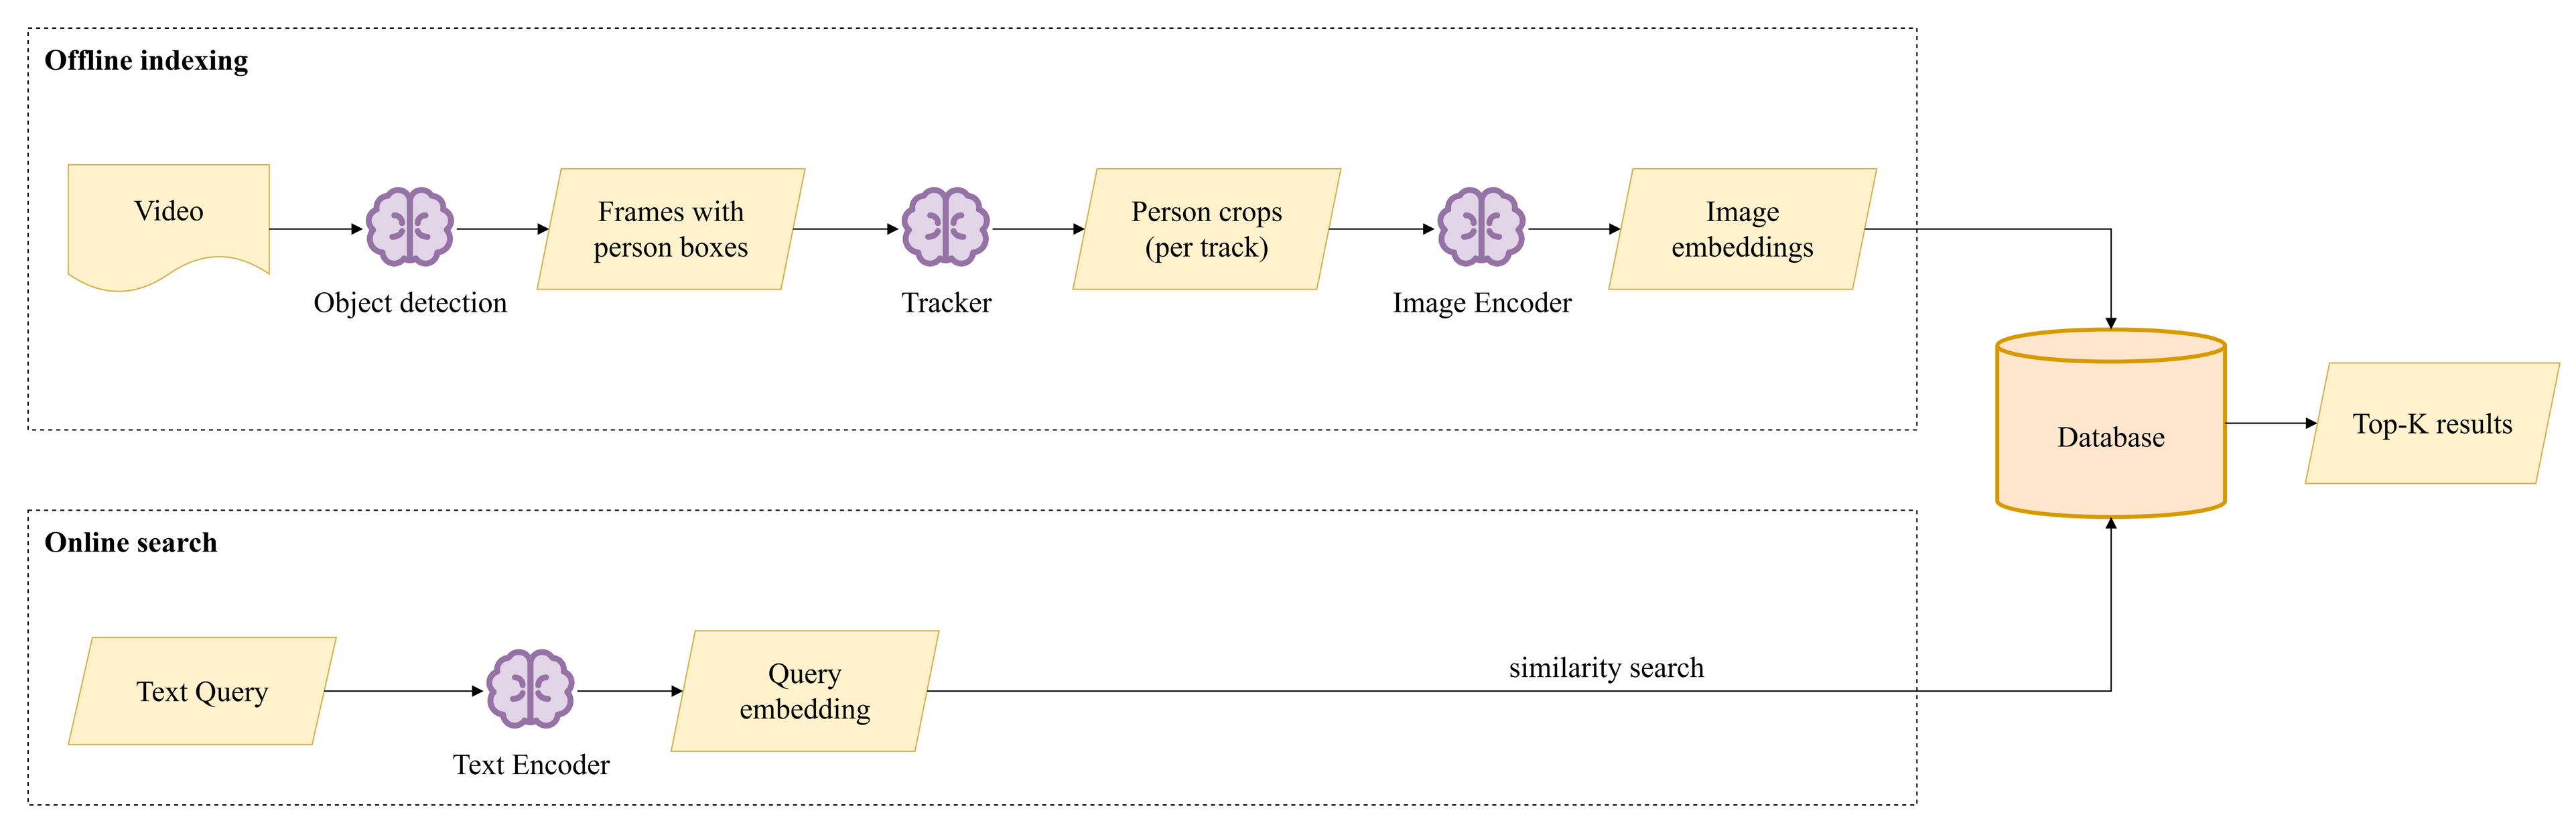
\includegraphics[width=\textwidth]{S23-overall-pipeline.png}
\caption[The pipeline as a template of replaceable blocks]{The pipeline as a template. Offline: video $\rightarrow$ object
detection $\rightarrow$ tracker $\rightarrow$ image encoder $\rightarrow$
database. Online: text query $\rightarrow$ text encoder $\rightarrow$ similarity
search against the same database. Every box is a slot for any detector, tracker
or encoder.}
\label{fig:r-overall}
\end{figure}

\subsection{Possible directions for improvement}
\label{sec:r-directions}
Table~\ref{tab:r-directions} compares the blocks by what each must achieve and how
it fails.

\begin{table}[H]
\centering
\begin{tabular}{@{}P{3.2cm}P{4.0cm}P{6.4cm}@{}}
\toprule
\textbf{Direction} & \textbf{Main requirement} & \textbf{Our consideration}\\
\midrule
Object detection & Detect people correctly & Errors propagate downstream.\\
\addlinespace
Tracking & Maintain identity across frames & Tracker errors can contaminate a
whole track.\\
\addlinespace
Image/text encoders and online search & Match the query to visual appearances &
Needs semantic generalisation and robustness to upstream errors, at the image
quality of deployed cameras.\\
\bottomrule
\end{tabular}
\caption[The three places where the pipeline can be improved]{The three places the pipeline can be improved, what each has to do, and
what that costs.}
\label{tab:r-directions}
\end{table}

Detection and tracking are well studied, and improving them mostly means a better
model in the slot. Their failures also reach the search block anyway: a missed
detection is a crop that never exists, and a merged track contains two people.

The search block alone must generalise from a sentence to an appearance, tolerate
the detector's and tracker's mistakes, and do both on deployed-camera crops; it is
also where the answer is decided. The work of this part is therefore placed there.
Given the two limits of CLIP above, the block needs a representation that can be
\emph{read}, attributes with their evidence, and a component able to weigh several
partly contradictory readings of one person. This is a reasoning problem over text,
which suits an LLM, as ZARA observed in another domain.

\subsection{ZARA: related work and inspiration}
\label{sec:r-zara}
The closest prior work is ZARA~\cite{li2025zara}, from which the reasoning pattern
is taken; the domain and the evidence are this project's own. ZARA's key idea is
that an LLM reasons poorly over raw numerical signals but well over \emph{textual}
evidence, so it first converts statistical patterns of the reference data into a
textual knowledge base and, at inference, retrieves the discriminative evidence for
the candidate classes (Figure~\ref{fig:r-zara}).

We keep this structure and change the domain. ZARA's statistics come from motion
signals; ours are human-readable person attributes extracted offline by Qwen-VL.
In ZARA, several sensors give complementary views of one activity; here, the
frames of one track give complementary views of one person. The difference is that
a tracker can group two people in one track, an upstream failure that ZARA's
sensors do not have (Section~\ref{sec:r-directions}).

The attribute statistics are not treated as ground truth, since Qwen-VL errs,
especially on real surveillance image quality and viewpoints, and the tracker adds
its own errors. They are given to an LLM as \emph{evidence to be reasoned over},
and the aggregated track-level reading re-ranks the candidates against the query:

\begin{center}
\small
\begin{tabular}{@{}ll@{}}
\toprule
ZARA & motion signals $\rightarrow$ statistical features $\rightarrow$
       multi-sensor evidence $\rightarrow$ LLM reasoning\\
Ours & person images $\rightarrow$ human-readable attributes $\rightarrow$
       multi-frame track evidence\\
     & \quad $\rightarrow$ LLM evidence aggregation $\rightarrow$ candidate
       re-ranking\\
\bottomrule
\end{tabular}
\end{center}

\begin{figure}[H]
\centering
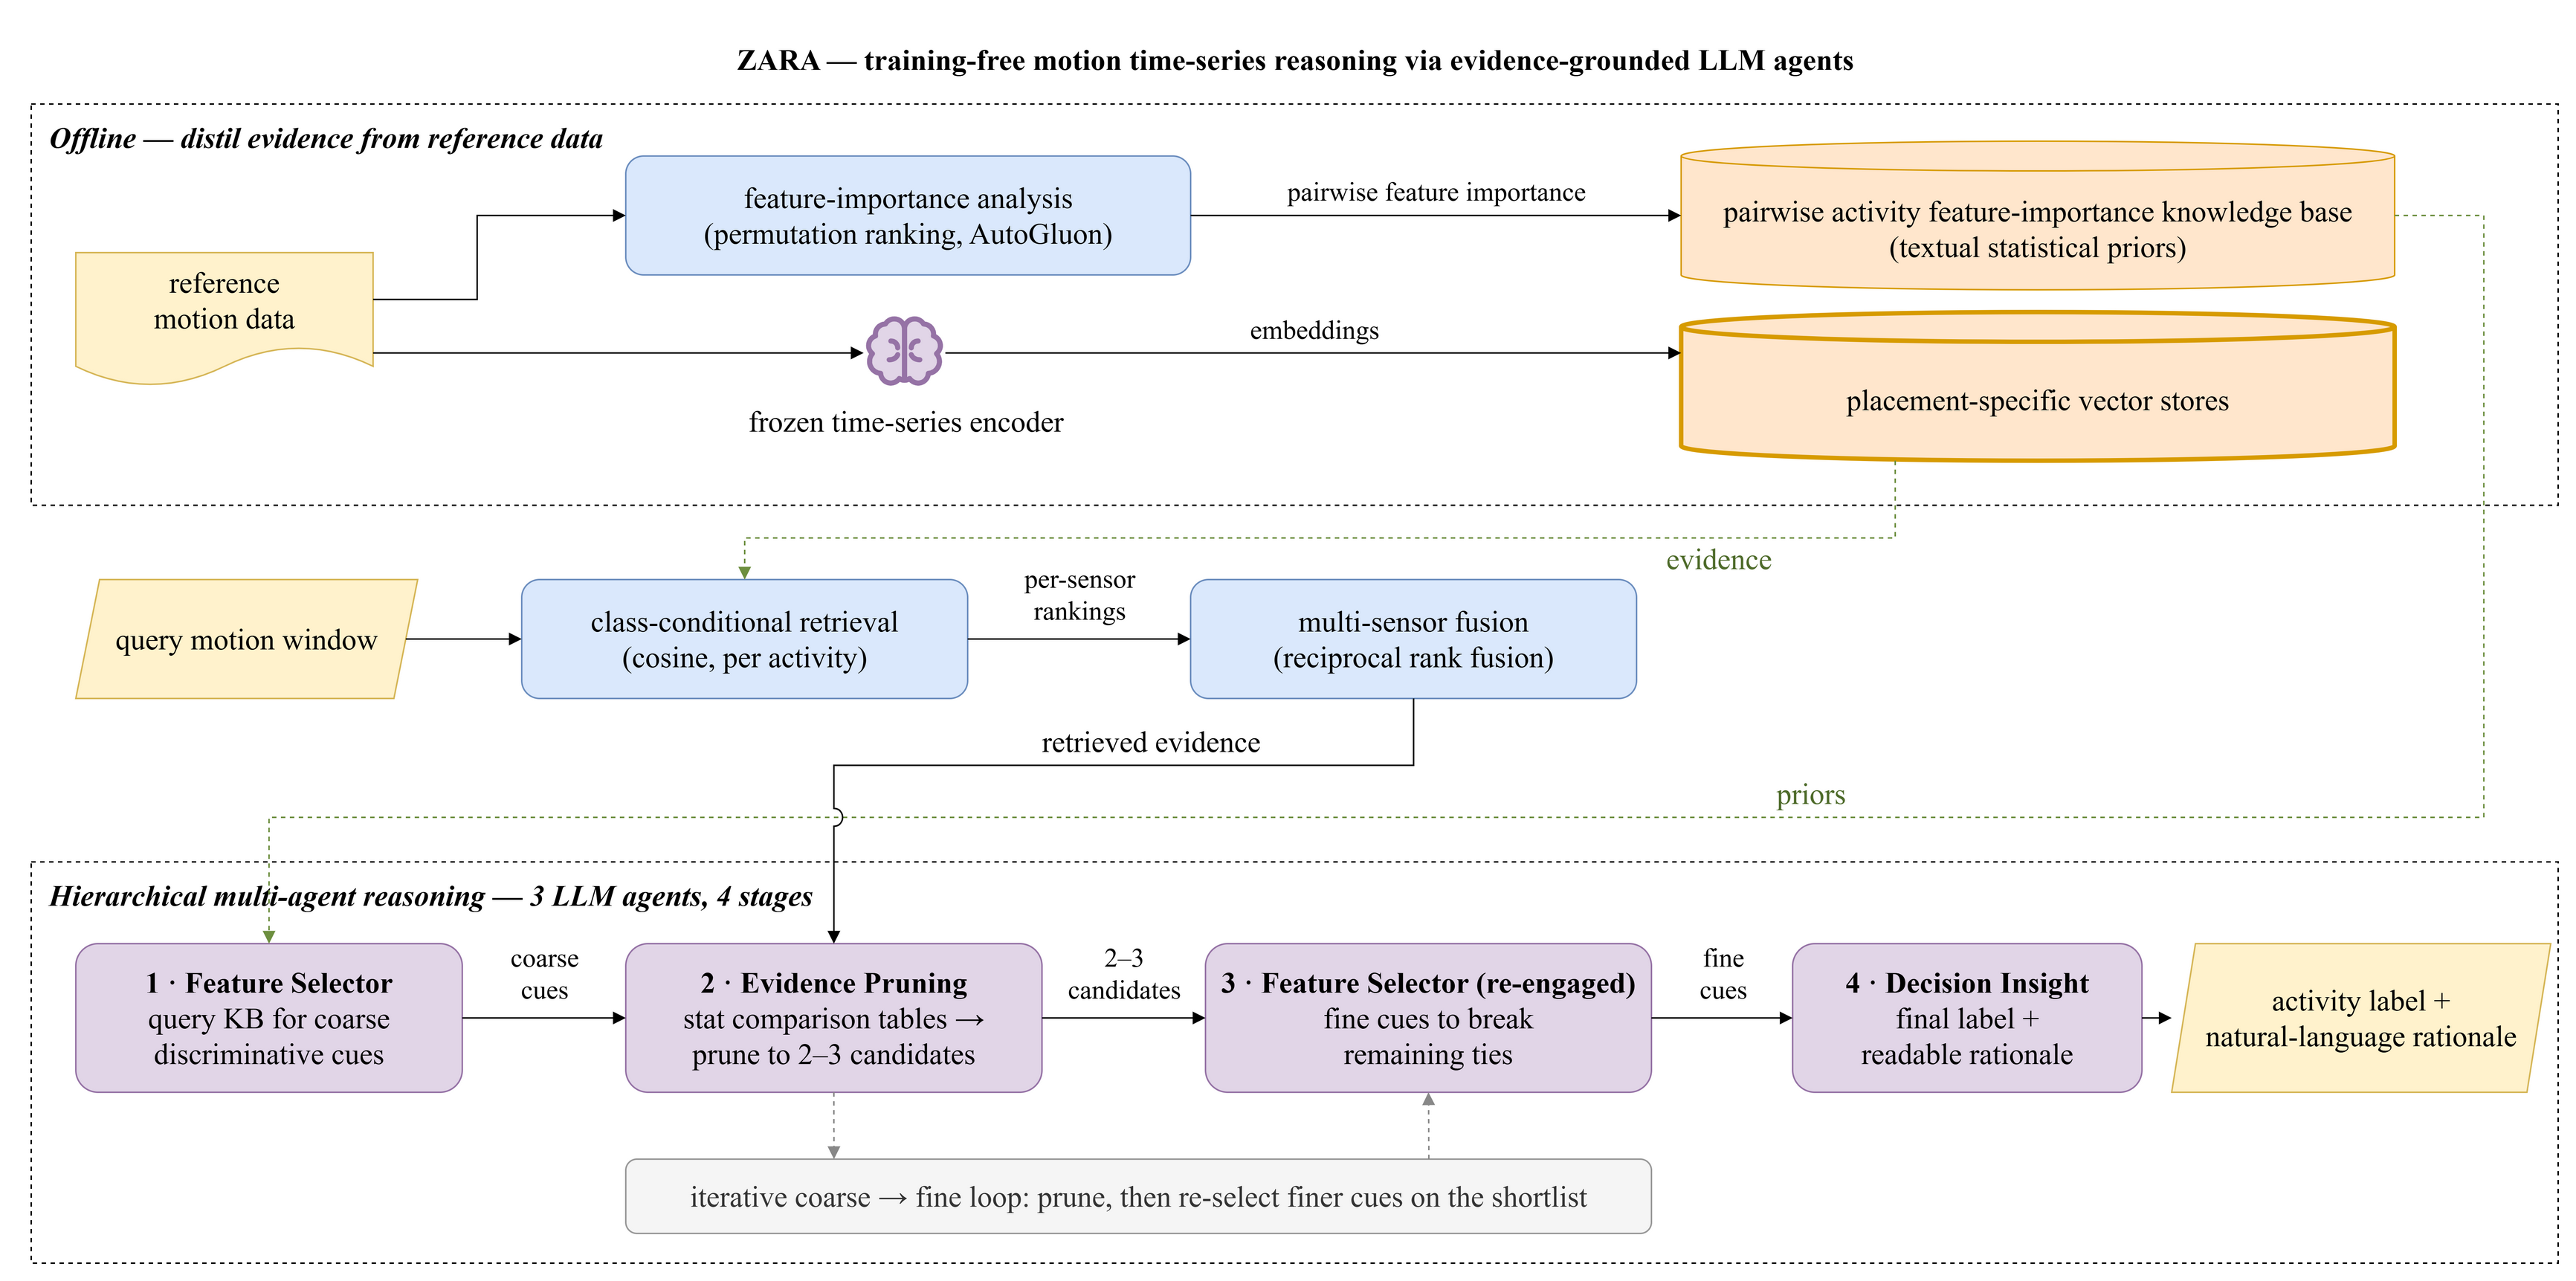
\includegraphics[width=\textwidth]{S26-zara.png}
\caption[ZARA's retrieval of discriminative evidence]{ZARA's retrieval of discriminative evidence for candidate classes, the
pattern this project adapts.}
\label{fig:r-zara}
\end{figure}

The coarse-to-fine iteration is also taken from ZARA: the funnel of
Section~\ref{sec:r-reasoning} prunes before it decides, with a coarse round over the
whole pool and a finer round over the survivors.

\section{System Overview}

\subsection{Filling the slots}
\label{sec:r-choices}
Table~\ref{tab:r-choices} puts a model into each block of Figure~\ref{fig:r-overall}.
The detector and tracker are established defaults, chosen so that they are not the
bottleneck, and are not studied further. In the search block, CLIP stays as the
\emph{base encoder} that builds the candidate pool, followed by an LLM-based
reasoning layer.

\begin{table}[H]
\centering
\begin{tabular}{@{}lll@{}}
\toprule
\textbf{Block} & \textbf{Choice} & \\
\midrule
Object detection            & YOLO11n                     & \cite{jocher2024yolo11}\\
Tracker                     & ByteTrack                   & \cite{zhang2022bytetrack}\\
Image/text encoder          & CLIP ViT-H/14 (laion2B), as the base encoder
                                                          & \cite{laion2022clipvith14}\\
Online search               & LLM-based reasoning layer over the CLIP pool & \\
Database, similarity search & Milvus                      & \cite{milvusdocs}\\
VLM (attribute describer)   & Qwen2.5-VL-3B-Instruct      & \cite{qwen2024qwen25vl3b}\\
LLM (reasoning)             & Gemini Flash-Lite 3.5       & \cite{googledeepmind-geminiflashlite}\\
\bottomrule
\end{tabular}
\caption{One model per slot. None of them is fine-tuned on this dataset.}
\label{tab:r-choices}
\end{table}

\subsection{Offline indexing}
\label{sec:r-offline}
In the indexing phase (Figure~\ref{fig:r-offline-new}), detection and tracking are
unchanged; the new element is that each tracked crop passes through \emph{two}
describers: CLIP for the retrieval embedding and Qwen2.5-VL-3B for the attribute
record. Both are stored under (video, track, frame), so a retrieved crop is joined
with its attributes and with the other frames of its track in one lookup.

\begin{figure}[H]
\centering
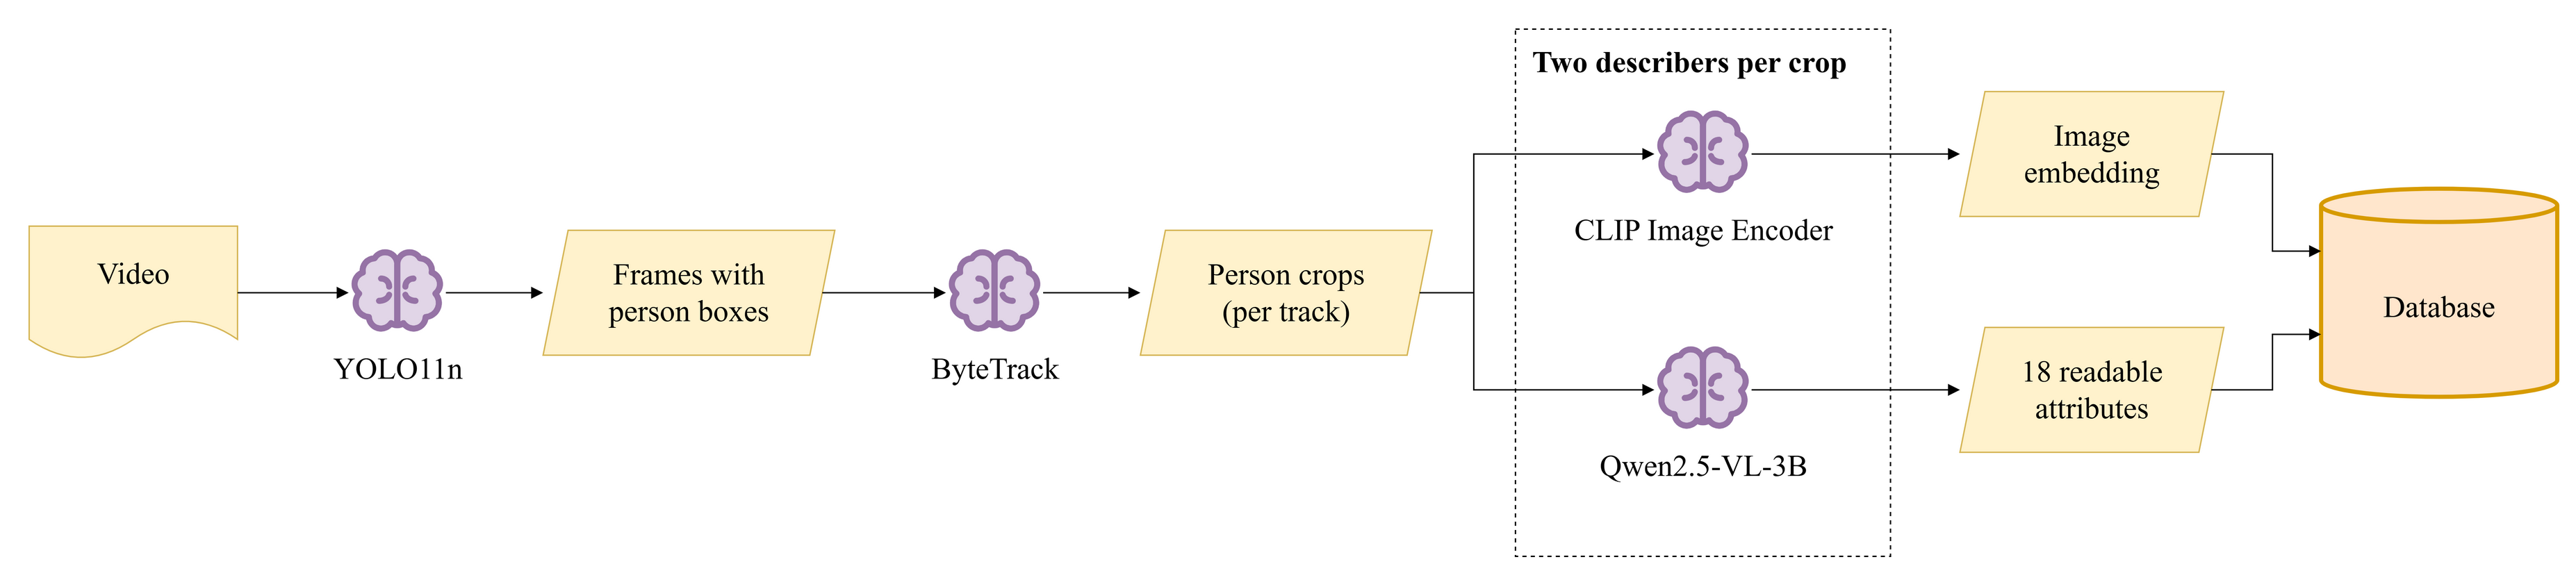
\includegraphics[width=\textwidth]{S31-offline-indexing.png}
\caption[Extended offline indexing with the attribute describer]{Extended offline indexing. The Qwen2.5-VL-3B branch turns each crop into
18 readable attributes alongside its embedding, which the reasoning stages need.}
\label{fig:r-offline-new}
\end{figure}

\subsection{Online search}
\label{sec:r-online}
In the search path (Figure~\ref{fig:r-online-full}), CLIP retrieval is unchanged,
but its output becomes an \emph{intermediate candidate pool}, which the multi-agent
reasoning block takes together with the original text to return the final top-$K$.

\begin{figure}[H]
\centering
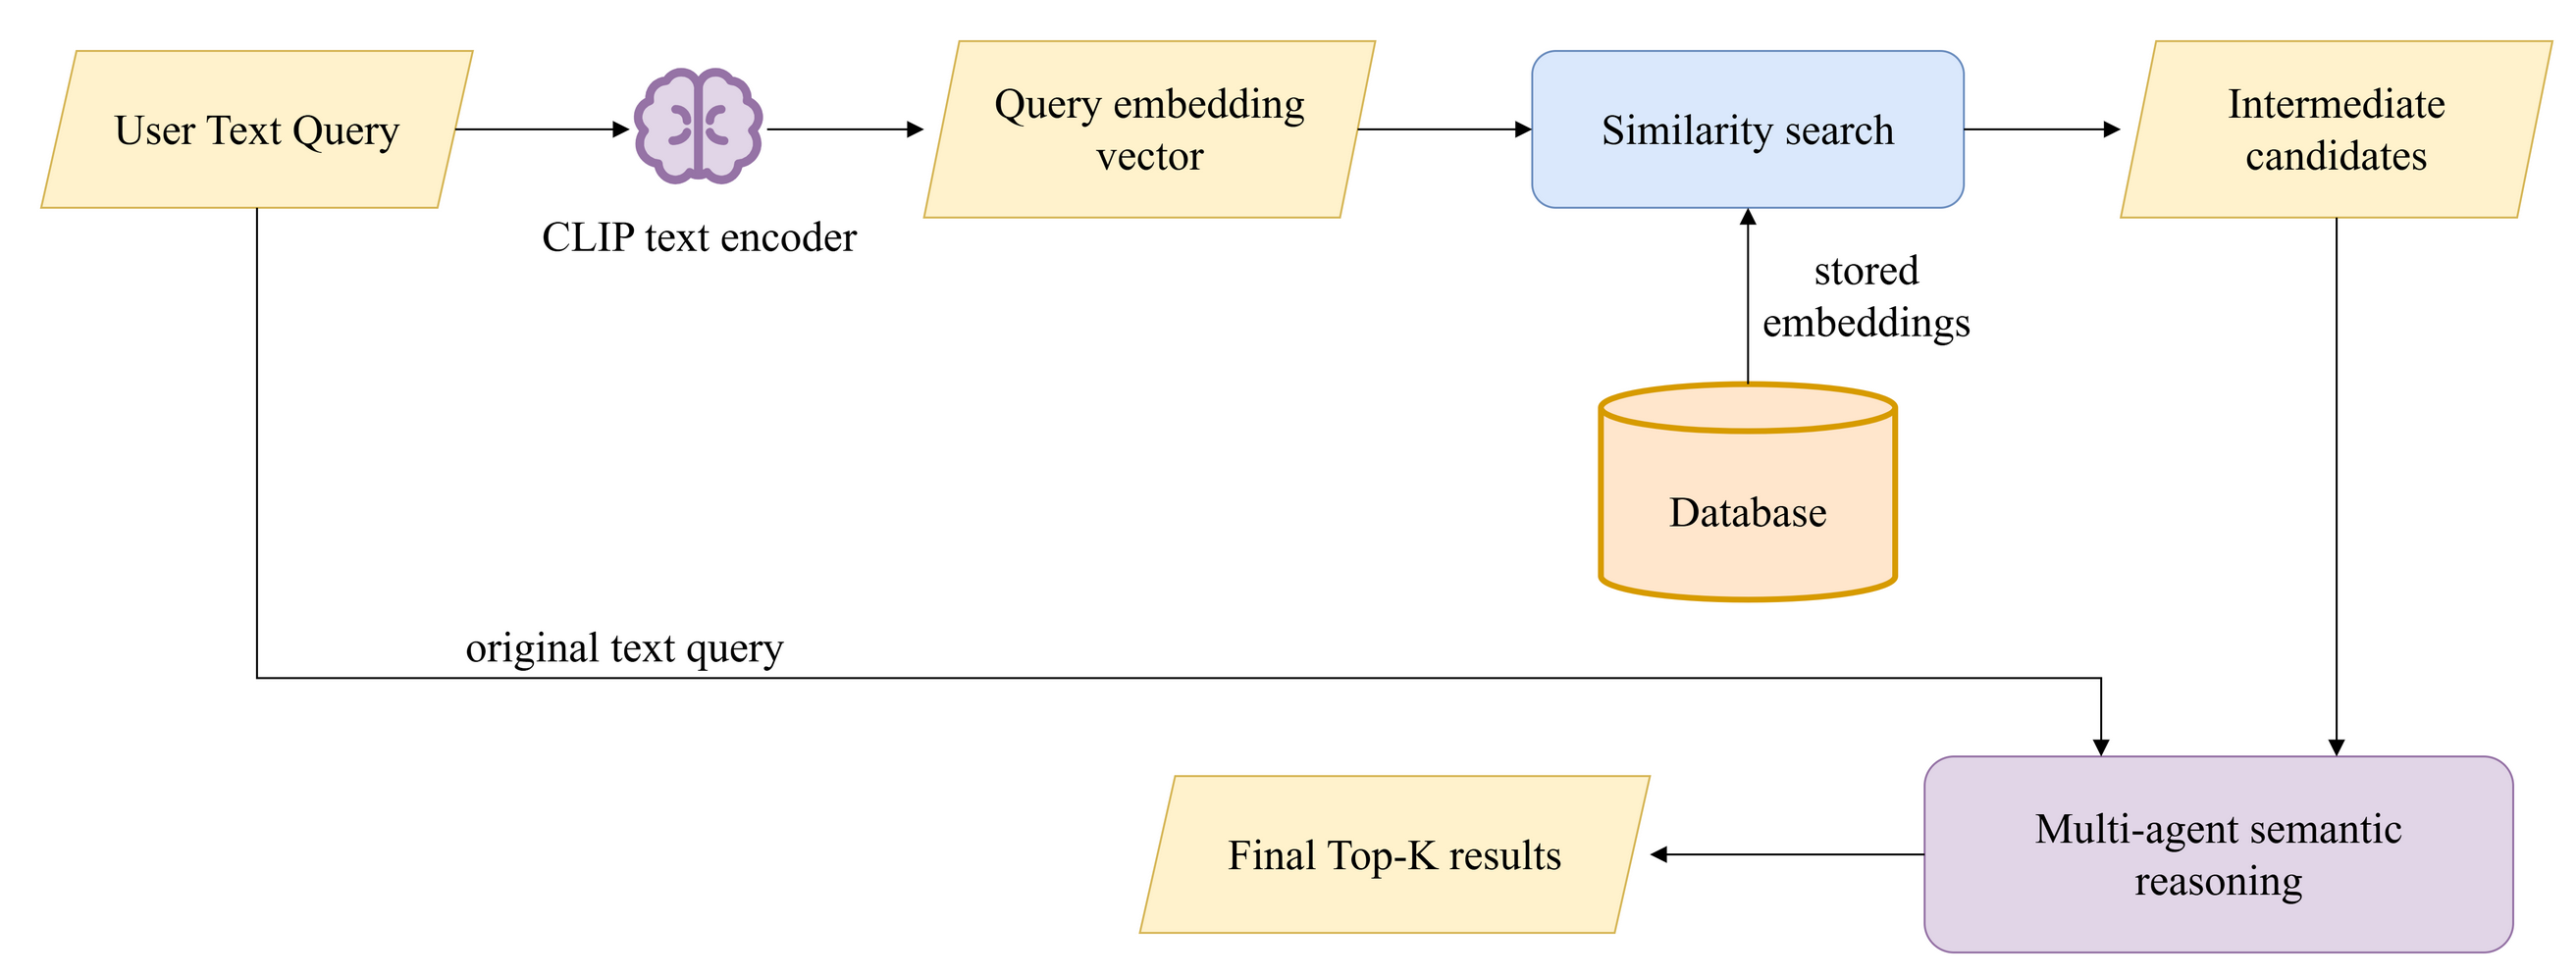
\includegraphics[width=0.95\textwidth]{S35-text-retrieval.png}
\caption[Online search with the reasoning layer]{Online search with the reasoning layer. CLIP produces the candidates and
the funnel orders them. The user's text reaches the reasoning block directly and
is not summarised by the retrieval stage.}
\label{fig:r-online-full}
\end{figure}

The reasoning layer can only reorder what retrieval gave it: a person missing from
the pool cannot be returned. Section~\ref{sec:r-metrics} therefore reports this
ceiling, \code{cap@75}, next to every recall number.

% ============================================================ 4 the index ===

% !TEX root = ../../main.tex
% Part II (Nguyen Huu Cuong) - merged from the research report (report_latex_v3), see MERGE_NOTES.md.
% Style pass 2026-09-30: em dashes and rhetorical sentences removed; technical content, numbers and references unchanged.
\chapter{Attribute Index and Multi-Agent Reasoning}
\label{chapter:r-reasoning}

\textit{This chapter describes the attribute index built offline with a vision-language model, and the multi-agent funnel that re-ranks the candidates of CLIP retrieval from that evidence.}

\section{The Attribute Index}

\subsection{Schema}
Each described crop carries the 18 attributes of Table~\ref{tab:r-attrs}. The
schema is deliberately centred on garments, since these are what a witness
usually describes. \at{carrying\_canon} is list-valued (a person can carry a
backpack \emph{and} a handbag); every other attribute is single-valued per crop,
although the same attribute read across a track often produces several values,
which is the signal the reasoning stages use.

\begin{table}[H]
\centering
\small
\begin{tabular}{@{}lll@{}}
\toprule
\textbf{Attribute} & \textbf{Region} & \textbf{Meaning}\\
\midrule
\at{gender}             & whole & apparent gender\\
\at{age\_group}         & head  & apparent age band\\
\at{build}              & whole & apparent build\\
\at{height\_class}      & whole & apparent height, words only\\
\at{hair\_color}        & head  & dominant hair colour\\
\at{hair\_style}        & head  & visible hairstyle\\
\at{upper\_inner\_type} & upper & the top worn under any outer layer\\
\at{upper\_inner\_color}& upper & the colour of that top\\
\at{upper\_outer\_type} & upper & the outermost upper garment (jacket, coat)\\
\at{upper\_outer\_color}& upper & the colour of that outer garment\\
\at{sleeves}            & upper & sleeve length\\
\at{pattern}            & upper & visible pattern on the upper body\\
\at{lower\_type}        & lower & lower-body garment\\
\at{lower\_color}       & lower & its colour\\
\at{lower\_length}      & lower & how far it reaches\\
\at{shoes\_type}        & feet  & footwear type\\
\at{shoes\_color}       & feet  & footwear colour\\
\at{carrying\_canon}    & whole & non-clothing objects carried (LIST-valued)\\
\bottomrule
\end{tabular}
\caption{The attribute schema, and the visual band each attribute is judged
from. The region column is a manual routing table: a wrong entry is invisible at
run time, because the evidence line still reads correctly but quotes the
sharpness of the wrong part of the body.}
\label{tab:r-attrs}
\end{table}

\subsection{Visual context}
Attributes alone cannot explain a disagreement. If one frame reads the top as red
and another as black, the useful question is whether the two frames were taken
under conditions that make this confusion likely. Every crop therefore also
carries numeric quality statistics, computed per band:

\begin{center}
\begin{tabular}{@{}ll@{}}
\toprule
\textbf{Band} & \textbf{Extent of the crop}\\
\midrule
\at{whole} & the entire crop\\
\at{head}  & the first 15\%\\
\at{upper} & the next 30\%\\
\at{lower} & the next 40\%\\
\at{feet}  & the last 15\%\\
\bottomrule
\end{tabular}
\end{center}

\noindent
Each band carries four numbers: sharpness, contrast, brightness and saturation.
Because \at{upper\_inner\_color} is routed to the \at{upper} band, a note about a
colour disagreement can cite the saturation of the upper body in the frames that
read red and in those that read black, giving a mechanism with its figure rather
than a guess.

\subsection{Three different counts}
The same attribute value can be counted in three ways. Confusing them is the
easiest mistake in this design, so the implementation keeps them as three
separate functions:

\begin{itemize}
\item The \emph{global prior} is the value's share over the \emph{whole index},
      with lists \emph{split}: a reading of \at{[red, white]} plus a reading of
      \at{red} gives red 66\% and white 33\% over three observations. This is
      the base rate against which rarity is judged.
\item The \emph{track distribution} is the set of readings of one track, kept
      \emph{whole}: the same two readings give ``red+white 50\%, red 50\%''.
      This is what the evidence reader quotes.
\item \emph{Membership} tells whether a query value \at{red} matches a frame that
      read \at{[red, white]}, which it does.
\end{itemize}

The local (pool) prior adds one more rule: it is computed over
\emph{deduplicated tracks}, not over pool crops. Two pool crops from the same
five-frame track give a five-frame statistic, not a ten-frame one. Without this
rule, a person retrieved many times would dominate the pool statistic simply
because the retriever returned that person several times.

\subsection{The image-quality problem, and why voting does not work}
\label{sec:r-noise}
Table~\ref{tab:r-noise} shows one real track, described over ten frames. It is
the motivating example for Section~\ref{sec:r-reasoning}.

\begin{table}[H]
\centering
\small
\begin{tabular}{@{}ll@{}}
\toprule
\textbf{Attribute} & \textbf{Across the 10 described frames}\\
\midrule
\at{gender}             & female 80\%, male 20\%\\
\at{age\_group}         & young adult 100\%\\
\at{build}              & slim 100\%\\
\at{height\_class}      & average height 80\%, average 20\%\\
\at{hair\_color}        & black 40\%, brown 30\%, blonde 30\% (split)\\
\at{hair\_style}        & short 50\%, straight 30\%, long+straight 20\% (split)\\
\at{upper\_outer\_type} & hoodie 20\%, not visible 80\% (split)\\
\at{upper\_outer\_color}& black 20\%, not visible 80\% (split)\\
\at{upper\_inner\_type} & sweater 70\%, tank top 10\%, not visible 20\%\\
\at{upper\_inner\_color}& gray 40\%, black 40\%, not visible 20\%
                          (tied, the aggregate is arbitrary)\\
\bottomrule
\end{tabular}
\caption{VLM noise on one track. A majority vote would report
\at{hair\_color}${=}$black on a 40/30/30 split, and would break the 40/40 tie
on \at{upper\_inner\_color} by whichever value the sort visited first.}
\label{tab:r-noise}
\end{table}

Three distinct problems appear in this track. Ties make the aggregate arbitrary.
Splits across near-synonyms (\at{short}, \at{straight}, \at{long+straight}) are
not a disagreement about the person but about the vocabulary. Occlusion
(\at{not visible} 80\%) is not a value: it is the absence of an observation, and
counting it as one would let an invisible garment outvote a visible one. A voting
aggregator cannot distinguish these cases; an LLM that is told what each form
means can.

% ========================================================= 5 the reasoning ==
\section{Multi-Agent Semantic Reasoning}
\label{sec:r-reasoning}

\subsection{The funnel}
Figure~\ref{fig:r-reasoning} shows the reasoning block. It keeps ZARA's
coarse-to-fine iteration (Section~\ref{sec:r-zara}), pruning first and deciding
second, with four agents run over two rounds:

\begin{enumerate}
\item The attribute-value selector (stage 1) chooses the attribute-value pairs to
      spend evidence on, from the knowledge base and the pool statistics.
\item The evidence pruning agent (stage 2A) reads, for every candidate and every
      selected pair, what this crop says and what the evidence around that
      reading looks like.
\item After the coarse cut ($75 \rightarrow 25$), a second selector (stage 3)
      works on the survivors, whose statistics have changed because the pool has.
\item The decision agent (stages 2B and 4B) ranks the candidates from the notes
      and returns the final ordering.
\end{enumerate}

\begin{figure}[H]
\centering
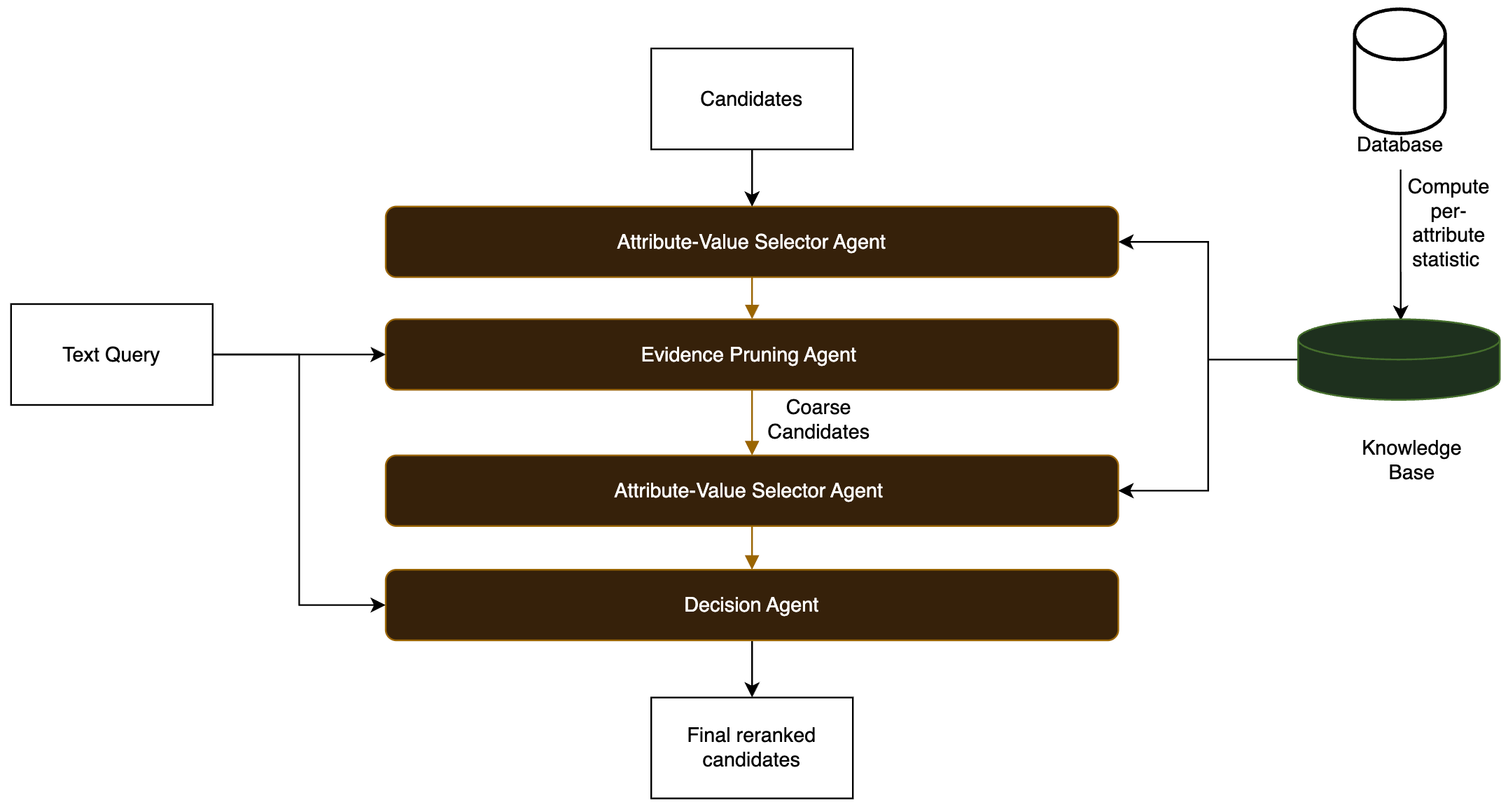
\includegraphics[width=0.95\textwidth]{reasoning-000.png}
\caption{The semantic reasoning block. The knowledge base supplies per-attribute
statistics to both selector calls; the text query reaches the pruning and
decision agents directly.}
\label{fig:r-reasoning}
\end{figure}

\paragraph{Why stage 0 is not in the funnel.} Neither the list above nor
Figure~\ref{fig:r-reasoning} shows the query analyst (stage 0), on purpose. The
funnel is the part that looks at candidates, and stage 0 never sees one. It is a
\emph{pre-run} over the query alone: it runs once per query, before the pool is
examined, and settles how each word of the query relates to each value used in
the index. Its output is a lookup table of relations, not a decision about any
candidate, and every stage of both rounds reads the same table. Drawing it as a
fifth agent inside the funnel would suggest that it takes part in pruning or
ranking, which it does not. Section~\ref{sec:r-stage0} describes it and explains
why it exists.

Two properties of this arrangement drive the prompt design. First, the coarse cut
cannot be undone: a candidate placed 26th in the first round can never be
returned, while a candidate ranked low in the second round still can. The two
mistakes are not symmetric, and the ranker is told so in round-dependent terms
(Section~\ref{sec:r-coverage}). Second, the second round renumbers the
candidates: the survivors are presented to stages 3 and 4 as candidates $1..M$
without their round-1 labels, so that the refine round is not anchored by the
ordering of the coarse round.

\subsection{Stage 0: query analyst}
\label{sec:r-stage0}
Before any candidate is seen, one call settles what the query asks of each
attribute. For every attribute in the index vocabulary it emits either
\code{NOT-CONSTRAINED} or one line per (index value, query value) pair with a
relation:

\begin{center}
\begin{tabular}{@{}ll@{}}
\toprule
\textbf{Relation} & \textbf{Meaning}\\
\midrule
\code{exact}     & interchangeable both ways; nothing gained or lost by writing either\\
\code{near}      & a plausible neighbour: what a describer might write for the same
                   thing\\
                 & under different light, from further away, or in motion\\
\code{far}       & a different value of the same kind, unlikely to be confused\\
\code{unrelated} & not the same property\\
\code{neutral}   & can neither confirm nor contradict (hides the attribute, too vague)\\
\bottomrule
\end{tabular}
\end{center}

\noindent
This is a statement about \emph{words}: the analyst sees no candidate, no image
and no statistic. The \code{near} relation matters most, because later stages use
it to tell a describer's mistake from a different person. The relations are
settled once per query and reused by every later stage, including the second
round, since asking the same question twice could produce two different answers.

\paragraph{Why a separate pre-run.} Every later stage has to decide whether what a
crop read agrees with what the query asked: the selector to weigh a pair, the
evidence reader to state where the query value stands, and the ranker to size a
conflict. Without stage 0, each of these calls would derive the relation between,
for example, \emph{navy} and \emph{black} on its own, inside a prompt already
crowded with statistics, and nothing would keep the answers consistent: the
evidence reader could treat a reading as a near match while the ranker treated
the same reading as a contradiction. Settling the relations once, from the words
alone, has three consequences.

\begin{itemize}
\item Consistency: one relation per (index value, query value) pair, read in the
      same way by stages 1 to 4 in both rounds.
\item Separation of concerns: a relation is a statement about language. Deciding
      it without candidates, images or statistics keeps it free of bias from how
      common a value is or from what the pool happens to contain; the later
      stages then reason about evidence, not vocabulary.
\item Cost: the call depends only on the query and the index vocabulary, so it is
      small, runs once per query, and is replayed from disk whenever the query is
      run again (Section~\ref{sec:r-engineering}).
\end{itemize}

\noindent
The most useful relation it produces is \code{near}: it lets the evidence reader
and the ranker treat a likely confusion of the describer (navy read as black in a
dim crop) differently from a real mismatch (navy read as red).

\subsection{Stage 1: attribute-value selector}
The selector chooses 4 to 10 attribute=value pairs with the highest expected
decision value, each with a one-sentence justification
(Figure~\ref{fig:r-selector}). It sees two tables: the \emph{global prior}, the
value's share over the whole index, and the \emph{local prior}, the pool's
distribution with the mean CLIP similarity and track stability per value
(Figure~\ref{fig:r-selector-work}).

\begin{figure}[H]
\centering
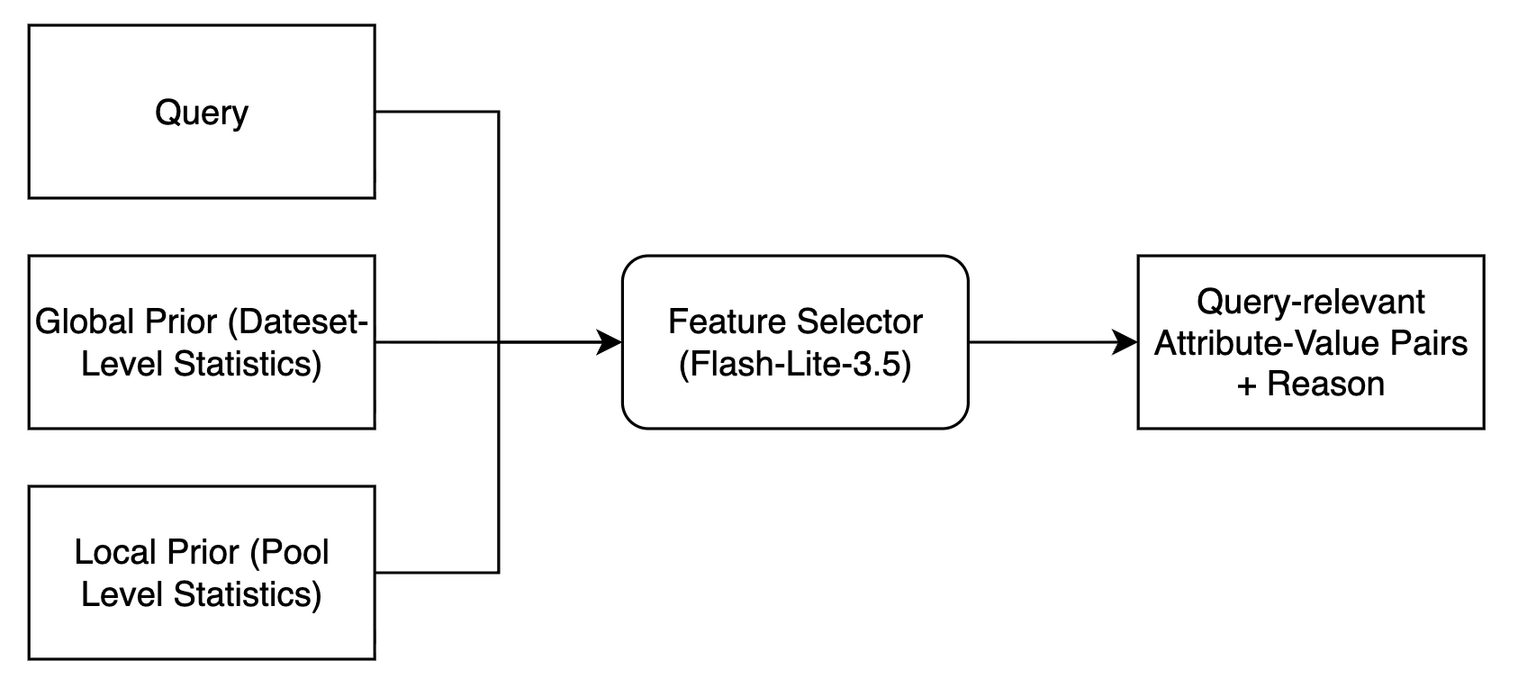
\includegraphics[width=0.90\textwidth]{selector-000.png}
\caption{The selector in the abstract. It decides \emph{where to look}, never what
is true: the output is a set of pairs with reasons, not a verdict.}
\label{fig:r-selector}
\end{figure}

\begin{figure}[H]
\centering
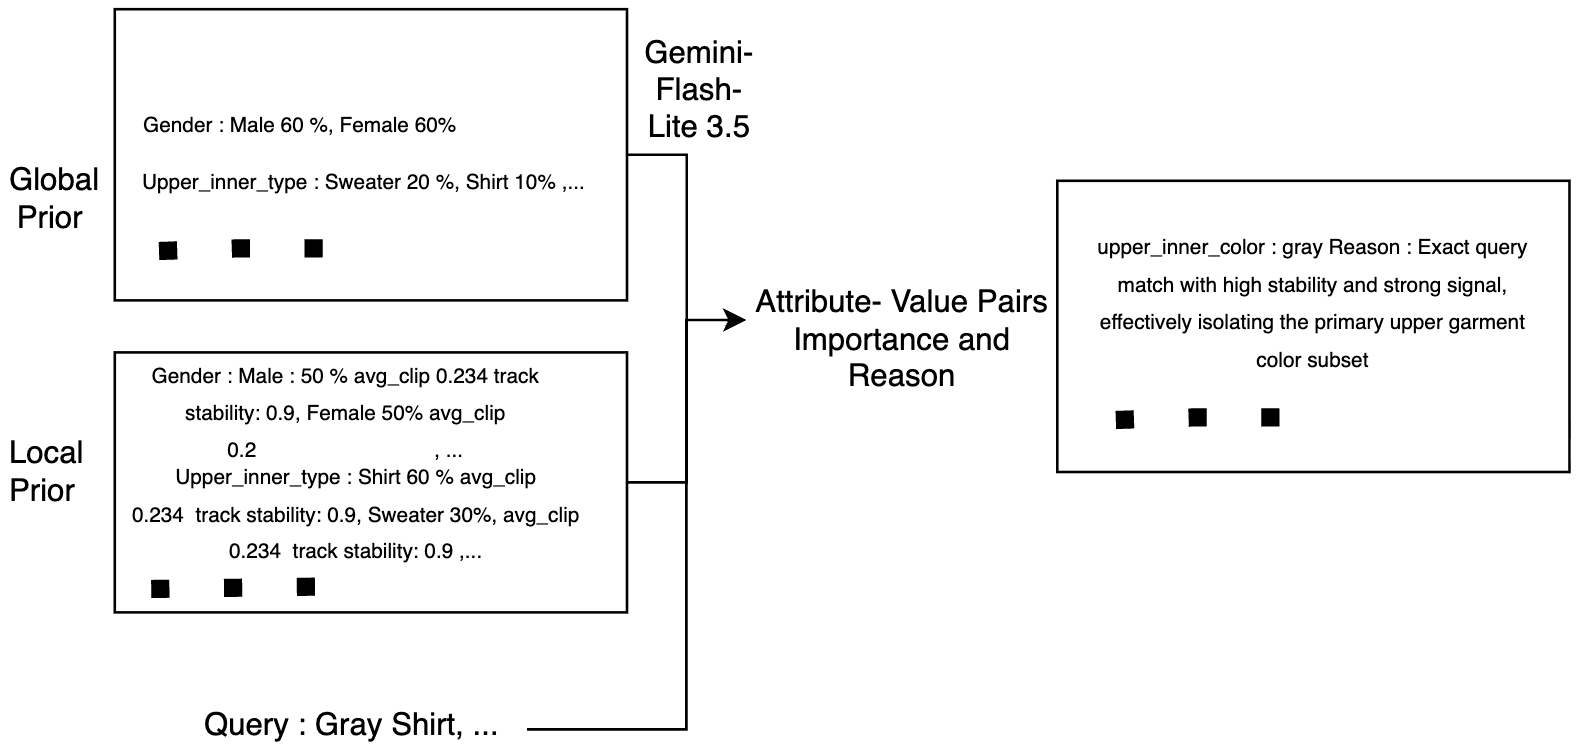
\includegraphics[width=0.97\textwidth]{selector_work-000.png}
\caption{The same stage with its real inputs and output: the two prior tables as
input, an attribute-value pair with its reason as output.}
\label{fig:r-selector-work}
\end{figure}

The prompt requires the choice to be made jointly across five dimensions, none of
which may decide alone: the query relation from stage 0; discrimination, that is,
how small a subset the value picks out; partitioning, how usefully it separates
competing groups; inspectability, the track stability qualified by the track
size, since a single-crop track has a stability of 1.00 by construction; and the
enrichment or depletion signal. A rare exact value can be highly decisive, a
common exact value can be weak, and a \emph{near} value can be worth a slot
because it explains an apparent mismatch.

One restriction was added after measurement: the selector's input is limited to
the attributes the query actually constrains. When shown the whole index, the
selector spent slots on attributes the query never mentioned, for which any
reading is equally consistent with the request.

\subsection{Stage 2A: evidence reader}
This is the most expensive stage and the core of the system. For each candidate
and each selected pair it writes exactly two lines: what \emph{this crop} read,
and a note about the evidence around that reading.

\begin{figure}[H]
\centering
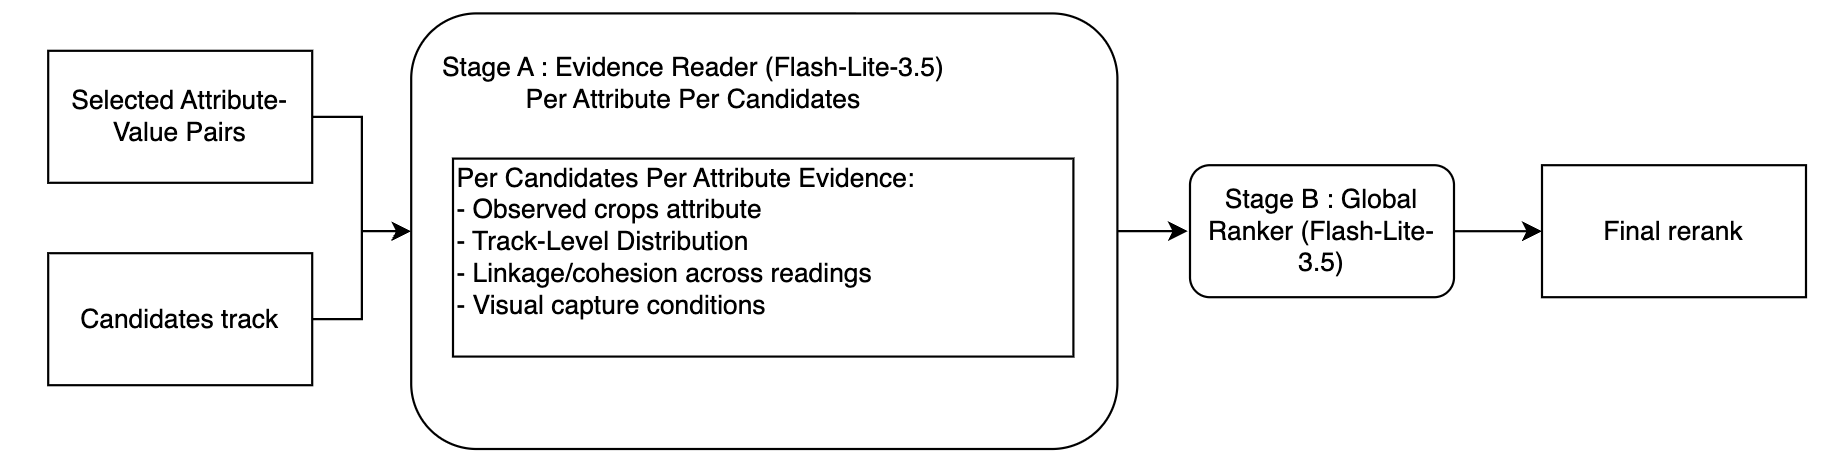
\includegraphics[width=0.95\textwidth]{pruning-000.png}
\caption{The evidence and decision stages in the abstract: stage A reads the
evidence per candidate and per attribute, and stage B ranks from what it wrote.}
\label{fig:r-pruning}
\end{figure}

\begin{figure}[H]
\centering
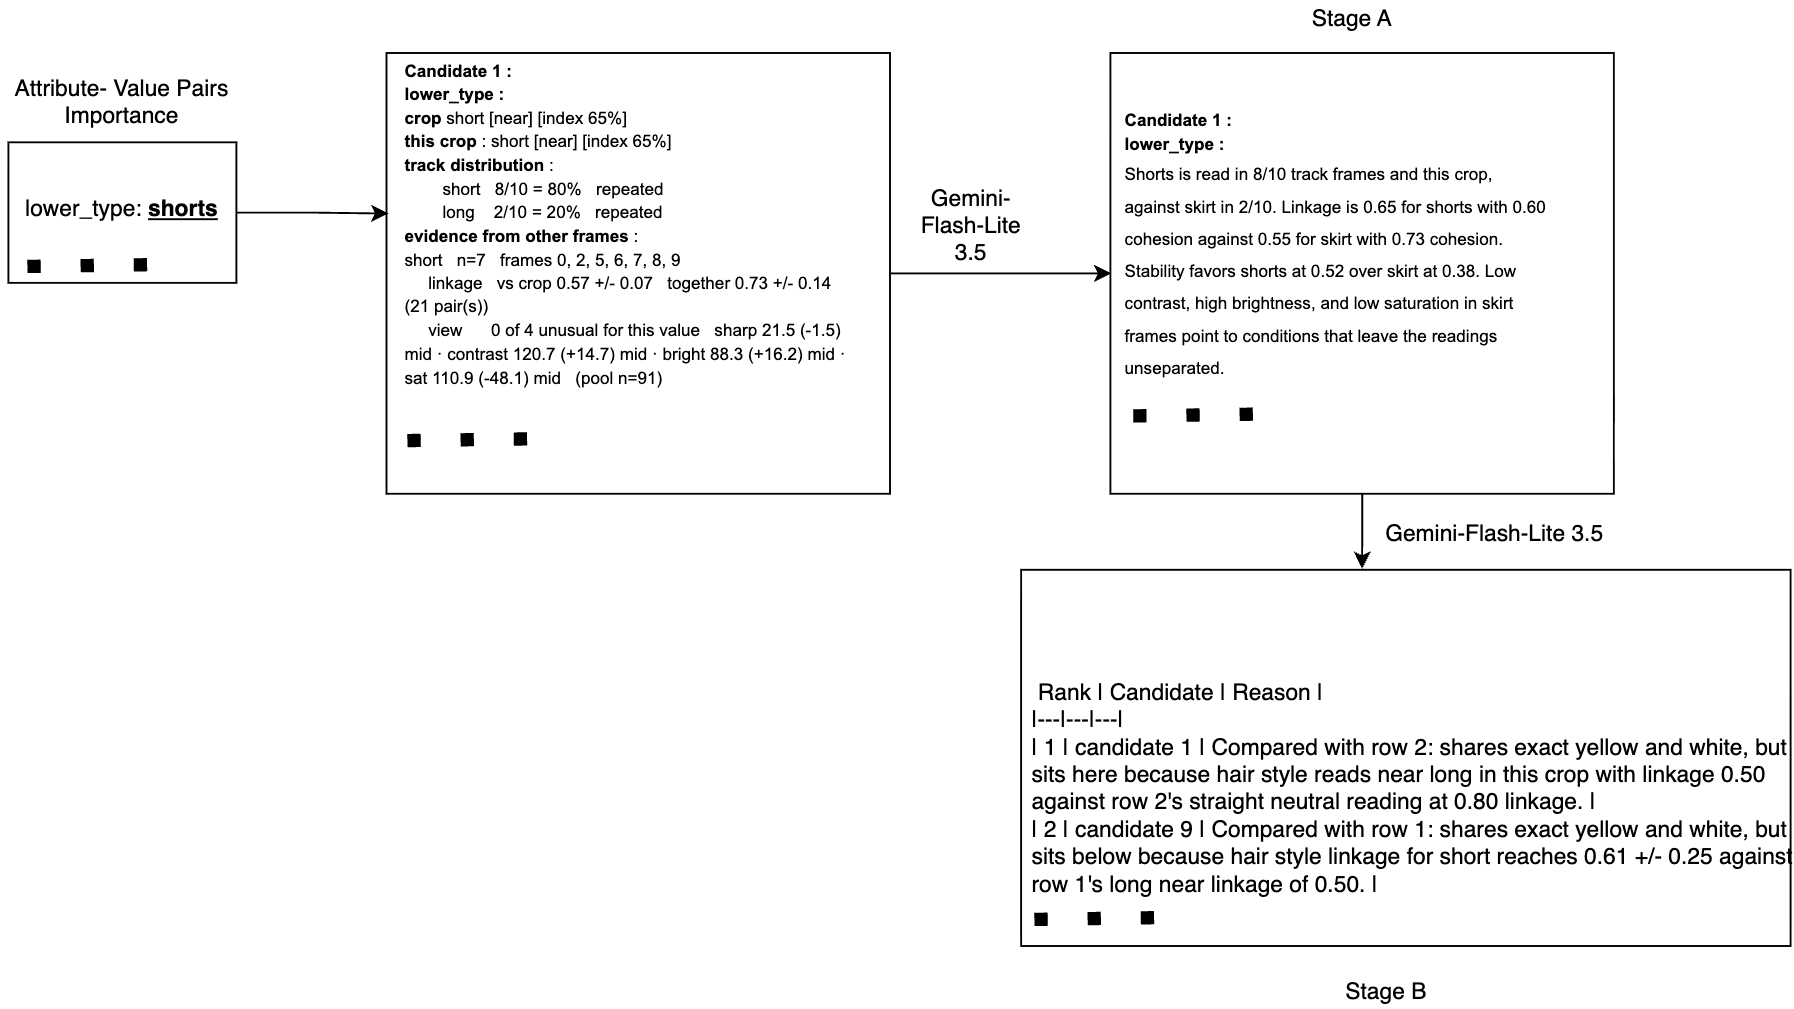
\includegraphics[width=0.97\textwidth]{pruning_work-000.png}
\caption{The same two stages at work: one rendered evidence block, the note the
reader writes from it, and the ranking the decision agent produces. Every figure
in the note appears in the block; nothing is recomputed or invented.}
\label{fig:r-evidence}
\end{figure}

The rendered block for one candidate and one pair contains at most:

\begin{itemize}
\item the crop's own reading, with its relation to the query value and its index
      share, for example \code{short [near] [index 65\%]};
\item the track distribution, such as \code{short 8/10 = 80\% repeated} and
      \code{long 2/10 = 20\% repeated}, kept whole as readings rather than split;
\item linkage and cohesion: how strongly the frames that read this value link to
      this crop (\code{vs crop 0.57 +/- 0.07}) and to each other
      (\code{together 0.73 +/- 0.14}), with the number of pairs the figure is
      computed from;
\item conditions: the quality figures for the relevant band, with the deviation
      from the pool's own distribution, for example
      \code{sharp 21.5 (-1.5) mid}, \code{contrast 120.7 (+14.7) mid},
      \code{bright 88.3 (+16.2) mid}, \code{sat 110.9 (-48.1) mid};
\item the view: whether this frame is unusual for its own value, printed only
      when at least two metrics fall outside that value's own range;
\item frame agreement: how much a quoted frame resembles the crop overall,
      \emph{excluding the attribute being judged}, so that a frame agreeing about
      the upper colour cannot be used to justify trusting it about the upper
      colour.
\end{itemize}

Four rules govern the note, each adopted after a measured failure:

\begin{enumerate}
\item The citation rule: never name a mechanism without the figure that shows it.
      Adding this rule reduced the invented causes in this stage from 19 to 0,
      and the mechanisms named without numbers to 0 of 82. It is the change with
      the clearest result in this pipeline, and it was also applied to the
      ranker.
\item The crop is a reference observation, not the truth. A frame agreeing with
      the crop is not evidence that the crop is right, because a tracker can group
      two people.
\item No deciding, ranking or averaging. The reader may not write
      \emph{correct}, \emph{winner}, \emph{most likely} or \emph{therefore the
      person is X}. Its task is to make the evidence readable; ordering is done by
      another stage with another prompt.
\item A length budget: one sentence of at most 25 words for an uncontested unit,
      and 40 to 95 words where the evidence is contested. Contested notes must be
      written in full: two to four channels with their figures, then a closing
      sentence saying where the evidence leaves the readings.
\end{enumerate}

Because a single call with 75 candidates would exceed the token window of the
free tier, stage 2A is split into three calls of 25 candidates. The split is sound
because stage 2A is independent across candidates and attributes: no note depends
on another. The batches are paced (Section~\ref{sec:r-engineering}).

\subsection{Stage 2B: the ranker}
The ranker sees the query and one note per attribute per candidate, and nothing
else: no per-attribute verdict, no score and no CLIP similarity. It ranks all $N$
candidates against each other and writes at least the top
$N_{\text{keep}} = \text{cap} + 5$ rows (30 of 75 in the coarse round, 15 of 25
in the refine round) as a markdown table with one reason per row.
$N_{\text{keep}}$ is a minimum, not a quota: the model is told to keep writing
while the evidence still separates one candidate from the next, and to stop when
it no longer does.

Three mechanisms shape the ordering.

\paragraph{Reliability, not direction.} Whether an attribute matches is the first
question; how much weight the reading can bear is the second, and the ordering is
based on the second. Ranking on direction produced 69 of 75 rows opening with
``Exact red top, shorts, female gender'', all of which was shared by the whole
pool and ordered nothing.

\paragraph{What each query value is worth.} The ranker receives a rarity table
once, at the top of its message: for every query value, its share in the index,
the \emph{typical} (median) share for that attribute, the most common share, and
the track stability. Each row ends with a label, \emph{decisive}
($\geq 5\times$ typical), \emph{moderate} ($\geq 1.5\times$) or \emph{almost
nothing}, and the ratio is printed next to it so that the label can be checked.
This was added after a measured failure: a candidate whose upper body was read as
green in every frame, green being rare, was ranked below candidates that only
matched a common colour, because no downstream stage carried any notion of
rarity.

\paragraph{The coverage floor.}
\label{sec:r-coverage}
The two rounds receive different instructions about absence, because their cuts
differ in kind.

\begin{itemize}
\item In the coarse round, PRESENT means read \emph{anywhere}: in one frame, as a
      minority reading, overshadowed by a competing value, in the track but not in
      this crop, or as a \code{[near]} value standing in for the query value. A
      present but weak reading ranks above an absent one. ABSENT is an evidence
      gap in either of its two forms: \emph{read nowhere in the track} (silence)
      and \emph{nothing closer than \code{[far]} read anywhere} (contradiction).
      The floor applies in one case only, the absence of a value that the rarity
      table calls \emph{decisive}. It is neither a count of matching attributes
      nor a score.
\item In the final round nothing lies below the cut any more, so there is nothing
      left to protect. A value read nowhere is still a reliable mismatch and
      should still push a candidate down; a single overshadowed frame is weak
      positive evidence, weighed against everything else, and not a floor.
\end{itemize}

\subsection{What the CLIP score is worth inside the pool}
\label{sec:r-clipscore}
The ranker receives the evidence notes and the query, and deliberately does
\emph{not} receive the CLIP similarity. This design decision is based on the
measurement in Table~\ref{tab:r-clipscore}.

CLIP does two jobs here, and only the second is in question. Building the pool is
not contested: the 75 candidates are CLIP's top 75 out of the whole index, and no
other part of the system could have produced them. Ordering inside the pool is
what stages 2B and 4B would inherit if the score were passed on, but the pool is
already the narrow top tail of a similarity distribution, so the spread that
ranked it against the \emph{index} may be almost gone \emph{within} the pool.

\begin{table}[H]
\centering
\begin{tabular}{@{}lr@{}}
\toprule
\textbf{Measured over the evaluated pools} & \textbf{Value}\\
\midrule
Mean pool similarity                        & 0.3272\\
Mean within-pool spread (rank 1 $-$ rank 75)& 0.0622\\
Mean within-pool standard deviation         & 0.0142\\
Median adjacent-rank gap                    & 0.0004 \ (2.7\% of one sd)\\
AUC, ground truth vs.\ rest of pool         & 0.601\\
Ground-truth $z$-score within pool          & $+1.24$ sd\\
\bottomrule
\end{tabular}
\caption{What the CLIP score separates \emph{inside} the 75-candidate pool. The AUC
is the probability that a ground-truth crop outranks a non-ground-truth crop there;
1.0 would mean the score alone sorts the pool perfectly, and 0.5 would be chance.
It is computed with ties taken into account, because many crops share the same
similarity to three decimals and counting a tie as a win would overstate the score
exactly where it is weakest.}
\label{tab:r-clipscore}
\end{table}

The three measurements point the same way. An AUC of 0.601 is weak separation:
inside the pool, the score is closer to chance than to a useful ordering. The
median gap between \emph{adjacent} ranks is 2.7\% of one standard deviation, so
ranks 8 and 20 are separated by numerical noise, and a ranker told to respect them
would be respecting noise. The ground truth does sit $+1.24$ standard deviations
above the pool mean, which is above average but not separated.

CLIP is therefore a good \emph{retriever}, since it produced this pool out of a
496-identity gallery, but a weak \emph{ranker of what it retrieved}. These are
different jobs, which is why they are measured separately here. Passing the score
into the ranking prompt would add little ordering information and would anchor the
ranker to the ordering it is meant to correct.

\subsection{Stages 3 and 4}
Stage 3 is the stage-1 prompt with one paragraph inserted: it selects
attribute-value pairs again over the 25 survivors, whose pool statistics differ
from those of the original 75. A value that was rare in the pool may now be shared
by all the survivors, and therefore useless for separating them. Stage 4A is the
evidence reader again, on the new pairs, and stage 4B is the ranker with the
\code{COVERAGE\_FINAL} section. The output of 4B, cut to 10, is the system's
answer.

\subsection{Engineering}
\label{sec:r-engineering}
Several implementation details are essential for reproducibility:

\begin{itemize}
\item Replay by byte-identical input. Every stage writes its rendered input and
      its reply to disk. Running an identity again replays from disk every stage
      whose input text is byte-identical, and resumes at the first stage without a
      saved answer. A run interrupted by a quota limit can therefore continue
      without repeating the calls already made.
\item Pacing. A rolling token-per-minute pacer holds back a call that would exceed
      the window, with a fixed 60-second gap between 2A batches, 180 seconds
      between identities, and exponential retry (60/120/240/480\,s) on errors 503
      and 429.
\item Robust parsing. A duplicate row in a ranking and a short reply are different
      failures and are reported separately; a candidate skipped in the middle of
      the list is appended in input order rather than dropped; and a ranking that
      cannot be parsed falls back to the CLIP order with a warning, because an
      empty round would score exactly like a wrong answer while hiding the parse
      failure.
\end{itemize}

% ================================================================= 6 setup ==

% !TEX root = ../../main.tex
% Part II (Nguyen Huu Cuong) - merged from the research report (report_latex_v3), see MERGE_NOTES.md.
% Style pass 2026-09-30: em dashes and rhetorical sentences removed; technical content, numbers and references unchanged.
\chapter{Experiments and Results}
\label{chapter:r-experiments}

\textit{This chapter presents the experimental setup on Market-1501, the results of the reasoning layer against the CLIP baseline with an analysis of what it rescues and what it loses, the ablations of its mechanisms, and the tooling that makes every number reproducible.}

\section{Experimental Setup}

\subsection{Dataset}
\label{sec:r-dataset}
The experiments use Market-1501~\cite{zheng2015market1501}, with the attribute
labels of the Market-1501\_\allowbreak Attribute project~\cite{lin2019market1501attr}. The
dataset contains 1501 identities, captured by six cameras on a university campus,
and its person boxes were produced by an automatic pedestrian detector rather than
drawn by hand.

\paragraph{Why Market-1501, and how it stands in for a tracker.} The reasoning
layer needs several crops of the same person, grouped together, so that the frames
of a track can agree or disagree about an attribute. Market-1501 provides this,
because every crop carries an identity label. Grouping crops by identity gives each
person a set of observations under different viewpoints, lighting, blur and
occlusion, which is what a tracker passes to the search block in the deployed
pipeline.

This is not a single-camera setting. A single-camera tracker links a person across
consecutive frames of one view, whereas the identity groups of Market-1501 span up
to six cameras. They therefore play the role of an \emph{ideal} tracker, one that
never switches identities, never merges two people, and follows a person across
cameras. The views inside one group differ more than the frames of a single-camera
track would, so disagreement between readings, which the funnel is built to reason
about, is more frequent rather than less. Market-1501 also carries third-party
hand annotation of attributes~\cite{lin2019market1501attr}, which makes an
attribute-level error analysis possible.

\paragraph{Why YOLO11n and ByteTrack are not in the experiment.} The experiment
tests the search block in isolation: the encoder, the retrieval of the candidate
pool, and the reasoning funnel behind it. Detection and tracking are left out on
purpose. Market-1501 already supplies the detected person crops and the identity
grouping, i.e.\ the outputs those two blocks would produce, so running YOLO11n and
ByteTrack on top would add nothing the dataset does not already provide, while
mixing their errors into the measurement. With them removed, every failure
reported in Section~\ref{sec:r-error} belongs to retrieval or to reasoning. The
cost of this isolation is that upstream errors are not measured at all;
Section~\ref{sec:r-limits} returns to this point. YOLO11n and ByteTrack remain the
chosen blocks of the deployed pipeline (Table~\ref{tab:r-choices}).

\paragraph{The 496-identity subset.} From the dataset and its hand annotation we
keep only the identities that are \emph{uniquely identified} by their annotated
attributes, that is, no other identity carries the same attribute vector. This
reduces 1501 identities to 496, and every rate in this part is drawn from that
population.

The reason is that the task has to be answerable from the description alone. If
two people in the gallery are described identically, a text query giving that
description has two correct answers while the annotation records only one, so a
system that returns the other is marked wrong although it is right. Removing those
identities removes a source of noise that the system cannot act on. It also makes
the benchmark \emph{easier} than the full 1501 identities, which must be taken into
account whenever these numbers are compared with published Market-1501 results,
since those are not computed on this subset.

\subsection{Models}
The models used in the experiment are the search-block entries of
Table~\ref{tab:r-choices}: CLIP ViT-H/14 (laion2B) as the base encoder, Milvus as
the vector database, Qwen2.5-VL-3B-Instruct as the attribute describer, and Gemini
Flash-Lite 3.5 as the reasoning LLM at thinking level HIGH for every stage.
Detection and tracking are supplied by the dataset itself
(Section~\ref{sec:r-dataset}), so YOLO11n and ByteTrack, the deployed pipeline's
choices for those blocks, are not run here.

No model is fine-tuned on this dataset, and every number below is zero-shot.
Sampling temperature is left at the provider default, following the guidance for
this model family.

\subsection{Funnel sizes and token budget}
To fit the token limits of the free Google AI Studio tier, we retrieve a cached
pool of 150 crops and use the top 75; the coarse round keeps 25 and the final
round returns 10. Stage 2A is split into three calls of 25 candidates.

\begin{table}[H]
\centering
\begin{tabular}{@{}lrr@{}}
\toprule
\textbf{Stage} & \textbf{Input tokens (est.)} & \textbf{Output tokens}\\
\midrule
1 and 3                  & $\sim$3k          & $\sim$200\\
2A (per split) and 4A    & 40k $\rightarrow$ 60k & 15k $\rightarrow$ 20k\\
2B                       & $\sim$60k         & $\sim$2k\\
4B                       & $\sim$20k         & $\sim$1k\\
\bottomrule
\end{tabular}
\caption{Per-call token budget. Output excludes thinking tokens, which are billed
as output and counted against the same rate window, so the real output load is
higher than this column. The reliable signal for a truncated reply is the API's
\code{finish\_reason}, not the reported output count.}
\label{tab:r-tokens}
\end{table}

\subsection{Baseline}
\paragraph{image-clip.} The baseline returns the top-10 \emph{crops} of the
75-candidate pool by cosine similarity, ungrouped, with repeats kept. Every table
reports this baseline. It is a like-for-like comparison: it returns the same kind
of result as the funnel, from the same pool.

\paragraph{A grouped baseline, considered and not reported.} An earlier sweep
also scored a \emph{track-naive} row, which assumes a perfect tracker: the pool's
crops are grouped by track, each person is scored by the maximum cosine over their
crops blended with how many of their crops surfaced
($0.7\,s_{\text{norm}} + 0.3\,c_{\text{norm}}$, both normalised within the
query's own pool), and the people are ranked by this score. It is not carried into
the results below, for two reasons. It answers a different question: it returns
ten distinct \emph{people} where image-clip and the funnel return ten
\emph{crops}, so its R@10 has a different denominator of opportunity. In addition,
on the earlier 44-identity sweep where it was measured, it tied image-clip exactly
at every $k$ and recovered no identity that CLIP's raw ordering had missed. This
cheaper grouping alternative to the reasoning layer therefore did not help.

\subsection{Metrics}
\label{sec:r-metrics}
R@$k$ is the fraction of queries whose ground-truth identity appears in the
returned top-$k$. Alongside it we report \code{cap@75}, how often the ground truth
was in the 75-crop pool at all. No reranking can exceed it, so the gap between
R@10 and \code{cap@75} is what reasoning could still gain, and the gap from
\code{cap@75} to 100\% can only be closed by retrieval. Reporting recall without
this ceiling would make a retrieval failure and a reasoning failure look the same.

% =============================================================== 7 results ==
\section{Results}

\subsection{Main comparison}

\begin{table}[H]
\centering
\begin{tabular}{@{}lccc@{}}
\toprule
\textbf{Method} & \textbf{R@1} & \textbf{R@5} & \textbf{R@10}\\
\midrule
CLIP (image-clip)   & \textbf{26.0\%} & 29.0\%          & 33.0\%\\
2 stages            & 23.0\%          & \textbf{46.0\%} & 53.0\%\\
4 stages            & 15.0\%          & 38.0\%          & \textbf{56.0\%}\\
\bottomrule
\end{tabular}
\caption{100 identities out of the 496-identity subset
(Section~\ref{sec:r-dataset}), pool of 75 candidates, zero-shot, one descriptive
phrasing each. At $n=100$ a percentage point is one identity.}
\label{tab:r-main}
\end{table}

Table~\ref{tab:r-main} gives three results.

First, the reasoning layer improves recall at depth. The four-stage funnel returns
the right person in the top 10 for 56 of 100 queries against CLIP's 33, that is,
23 more identities, from reranking alone, with no fine-tuning and no change to
retrieval. At R@5 the gain of the four-stage funnel is smaller, 9 points (38.0\%
against 29.0\%); the two-stage variant gains 17 points there (46.0\% against
29.0\%).

Second, the funnel is worse at the first rank. CLIP is the best method at R@1 (26
against 23 and 15). This is not a rounding effect: the funnel is consistently
better at placing the right person somewhere in the top ten and consistently worse
at placing them first. Section~\ref{sec:r-lost} shows where this happens.

Third, the refine round trades precision for depth. Two stages are better at R@1
and R@5, four stages at R@10. The second round moves into the top 10 candidates
that the coarse round had placed below it, rescuing three more identities, while
costing eight identities at R@1 and eight at R@5. Which of the two rounds should
decide rank 1 remains an open question of the project: the coarse ranker sees 75
candidates with sparse evidence, and the refine ranker sees 25 with dense
evidence.

\subsection{What the funnel changed: rescued and lost}
\label{sec:r-lost}
A recall figure combines two opposite effects. Table~\ref{tab:r-lost} separates
them: of the 33 identities CLIP already had in its top 10, how many survived; and
of the 67 it missed, how many the funnel recovered.

\begin{table}[H]
\centering
\begin{tabular}{@{}lcccc@{}}
\toprule
\textbf{Record} & \textbf{n} & \textbf{Lost} & \textbf{Rescued} & \textbf{No pool}\\
\midrule
2 stages & 100 & 5/33 \ (15\%) & 25/67 \ (37\%) & 3/100\\
4 stages & 100 & 5/33 \ (15\%) & 28/67 \ (42\%) & 3/100\\
\bottomrule
\end{tabular}
\caption{Lost: inside CLIP's top 10, not in the funnel's. Rescued: outside CLIP's
top 10, inside the funnel's. No pool: the ground truth was not among the 75
retrieved crops at all, so no reranking could have returned it.}
\label{tab:r-lost}
\end{table}

The table reproduces Table~\ref{tab:r-main} exactly, which confirms that it
measures the same thing: $33 - 5 + 28 = 56$ for four stages and $33 - 5 + 25 = 53$
for two.

The rescue rate is the main result: 42\% of the identities that CLIP could not
find in its top ten are found by reasoning over attributes, on a pool that CLIP
itself produced. The loss rate is the cost: about one in seven of the identities
already found by retrieval is pushed out. The ceiling is also close: only 3 of 100
ground truths were never retrieved, so 97 of the 100 identities could have been
returned; 56 of them are, and the other 41 (41\% of the sample) are lost somewhere
inside the funnel. The 3 identities outside the pool are not part of these 41,
since no reranking could have returned them. The remaining room for improvement is
therefore in the ranking, not in retrieval.

The loss count is also the same for two and four stages (5 in both), while the
rescue count differs (25 against 28). The refine round adds rescues without adding
losses at the top-10 boundary; its cost appears at R@1 and R@5, inside the top ten.

\subsection{Where the losses happen}
\label{sec:r-lostwhere}
The five lost identities were traced through both rounds. Table~\ref{tab:r-lostwhy}
gives, for each, the rank assigned by CLIP and by each round.

\begin{table}[H]
\centering
\small
\begin{tabular}{@{}ccllp{4.6cm}@{}}
\toprule
\textbf{Candidate} & \textbf{CLIP} & \textbf{Stage 2} & \textbf{Stage 4} &
\textbf{Where it went}\\
\midrule
1 & 1 & 9/73  & 16 & the REFINE round put it 16 of 23\\
2 & 1 & 27/74 & n/a & LOST AT THE COARSE CUT (rank 27 $>$ 25)\\
3 & 1 & 15/75 & 15 & the REFINE round put it 15 of 25\\
4 & 1 & 7/74  & 22 & the REFINE round put it 22 of 24\\
5 & 6 & 30/73 & n/a & LOST AT THE COARSE CUT (rank 30 $>$ 25)\\
\bottomrule
\end{tabular}
\caption{The five identities CLIP had in its top 10 and the funnel did not
return. `Stage 2' is the coarse round's rank out of the candidates it ranked;
`n/a' in stage 4 means the refine round never saw that candidate.}
\label{tab:r-lostwhy}
\end{table}

Two were cut by the coarse round, at ranks 27 and 30 against a cut of 25. These
were near misses, but they cannot be recovered, because stages 3 and 4 never see
them. Three survived the coarse round and were then pushed out by the refine round,
one of them from rank 7 to rank 22. Four of the five were at CLIP rank 1.

That the refine round causes most of the losses is consistent with
Table~\ref{tab:r-main}, where the second round costs R@1 and R@5 while gaining
R@10. It is also why the coarse and refine rounds receive \emph{different}
instructions about absence (Section~\ref{sec:r-coverage}): the coarse cut cannot be
undone and the refine cut can, so the two mistakes are not symmetric and the
prompts should not treat them alike.

\subsection{Is the ranker the bottleneck? A targeted re-run}
\label{sec:r-rerun}
The losses in Table~\ref{tab:r-lostwhy} are ranking failures by construction: the
right person was retrieved, described and ranked, but not high enough. They are
therefore the one set on which the question \emph{``is the small model the
limitation?''} can be asked directly.

The five were re-run with only the ranking stages switched to a larger model
(Gemini Flash 3.8 in place of Flash-Lite 3.5). Everything else was held fixed:
stages 0, 1 and 2A were \emph{replayed} from the original run's saved replies
rather than sent again, so the new ranker read exactly the same evidence as the old
one. Stages 3 and 4A were run again, because their inputs change as soon as the
coarse ranking does.

\begin{table}[H]
\centering
\small
\begin{tabular}{@{}cclll@{}}
\toprule
\textbf{Identity} & \textbf{CLIP} & \textbf{Stage 2} & \textbf{Stage 4} &
\textbf{Result}\\
\midrule
1 & 1 & 9 $\rightarrow$ 7 of 73  & 16 $\rightarrow$ 8 of 24 & FIXED\\
2 & 1 & 27 $\rightarrow$ 1 of 74 & n/a $\rightarrow$ 1 of 25 & FIXED\\
3 & 1 & 15 $\rightarrow$ 3 of 75 & 15 $\rightarrow$ 1 of 25 & FIXED\\
4 & 1 & 7 $\rightarrow$ 14 of 74 & 22 $\rightarrow$ 14 of 25 & STILL WRONG\\
5 & 6 & 30 $\rightarrow$ 1 of 73 & n/a $\rightarrow$ 1 of 24 & FIXED\\
\bottomrule
\end{tabular}
\caption{The five lost identities re-ranked by a larger model at stages 2B and 4B
only. `Stage 2' and `Stage 4' read \emph{before} $\rightarrow$ \emph{after}.}
\label{tab:r-rerun}
\end{table}

Four of the five are recovered, and three of them reach rank 1 of the refine
round. Both coarse-cut losses (candidates 2 and 5) pass the cut easily once a
larger model does the coarse ranking, moving from 27 to 1 and from 30 to 1. The
one that stays wrong, candidate 4, is also the one that the original refine round
demoted the most.

This indicates that these losses came from the capacity of Flash-Lite at the
ranking stages, not from the evidence. The notes were sufficient, but the small
model did not use them well enough.

This result has one important limitation. The five identities were selected using
the ground truth: they are exactly the queries that the original run got wrong
while CLIP got them right. The experiment therefore answers whether the ranker is
the bottleneck \emph{on these failures}. It does not show what the system would
score with the larger model, which only a full sweep can measure, and these four
recoveries must not be added to Table~\ref{tab:r-main}.

\subsection{Case studies}

\paragraph{A lost case (Figure~\ref{fig:r-case-lost}).}
Query: \emph{``A teenage man, with long hair, wearing a short-sleeve red top and
white trousers.''} The ground truth is at CLIP rank 1. The reasoning layer keeps
red tops throughout the ten results it returns, so the garment evidence is used,
but the person it returns first is a different individual in a similar red top,
and the correct identity falls out of the top ten. This is a ranking failure with
correct evidence behind it, of the kind counted in Table~\ref{tab:r-lostwhy}.

\begin{figure}[H]
\centering
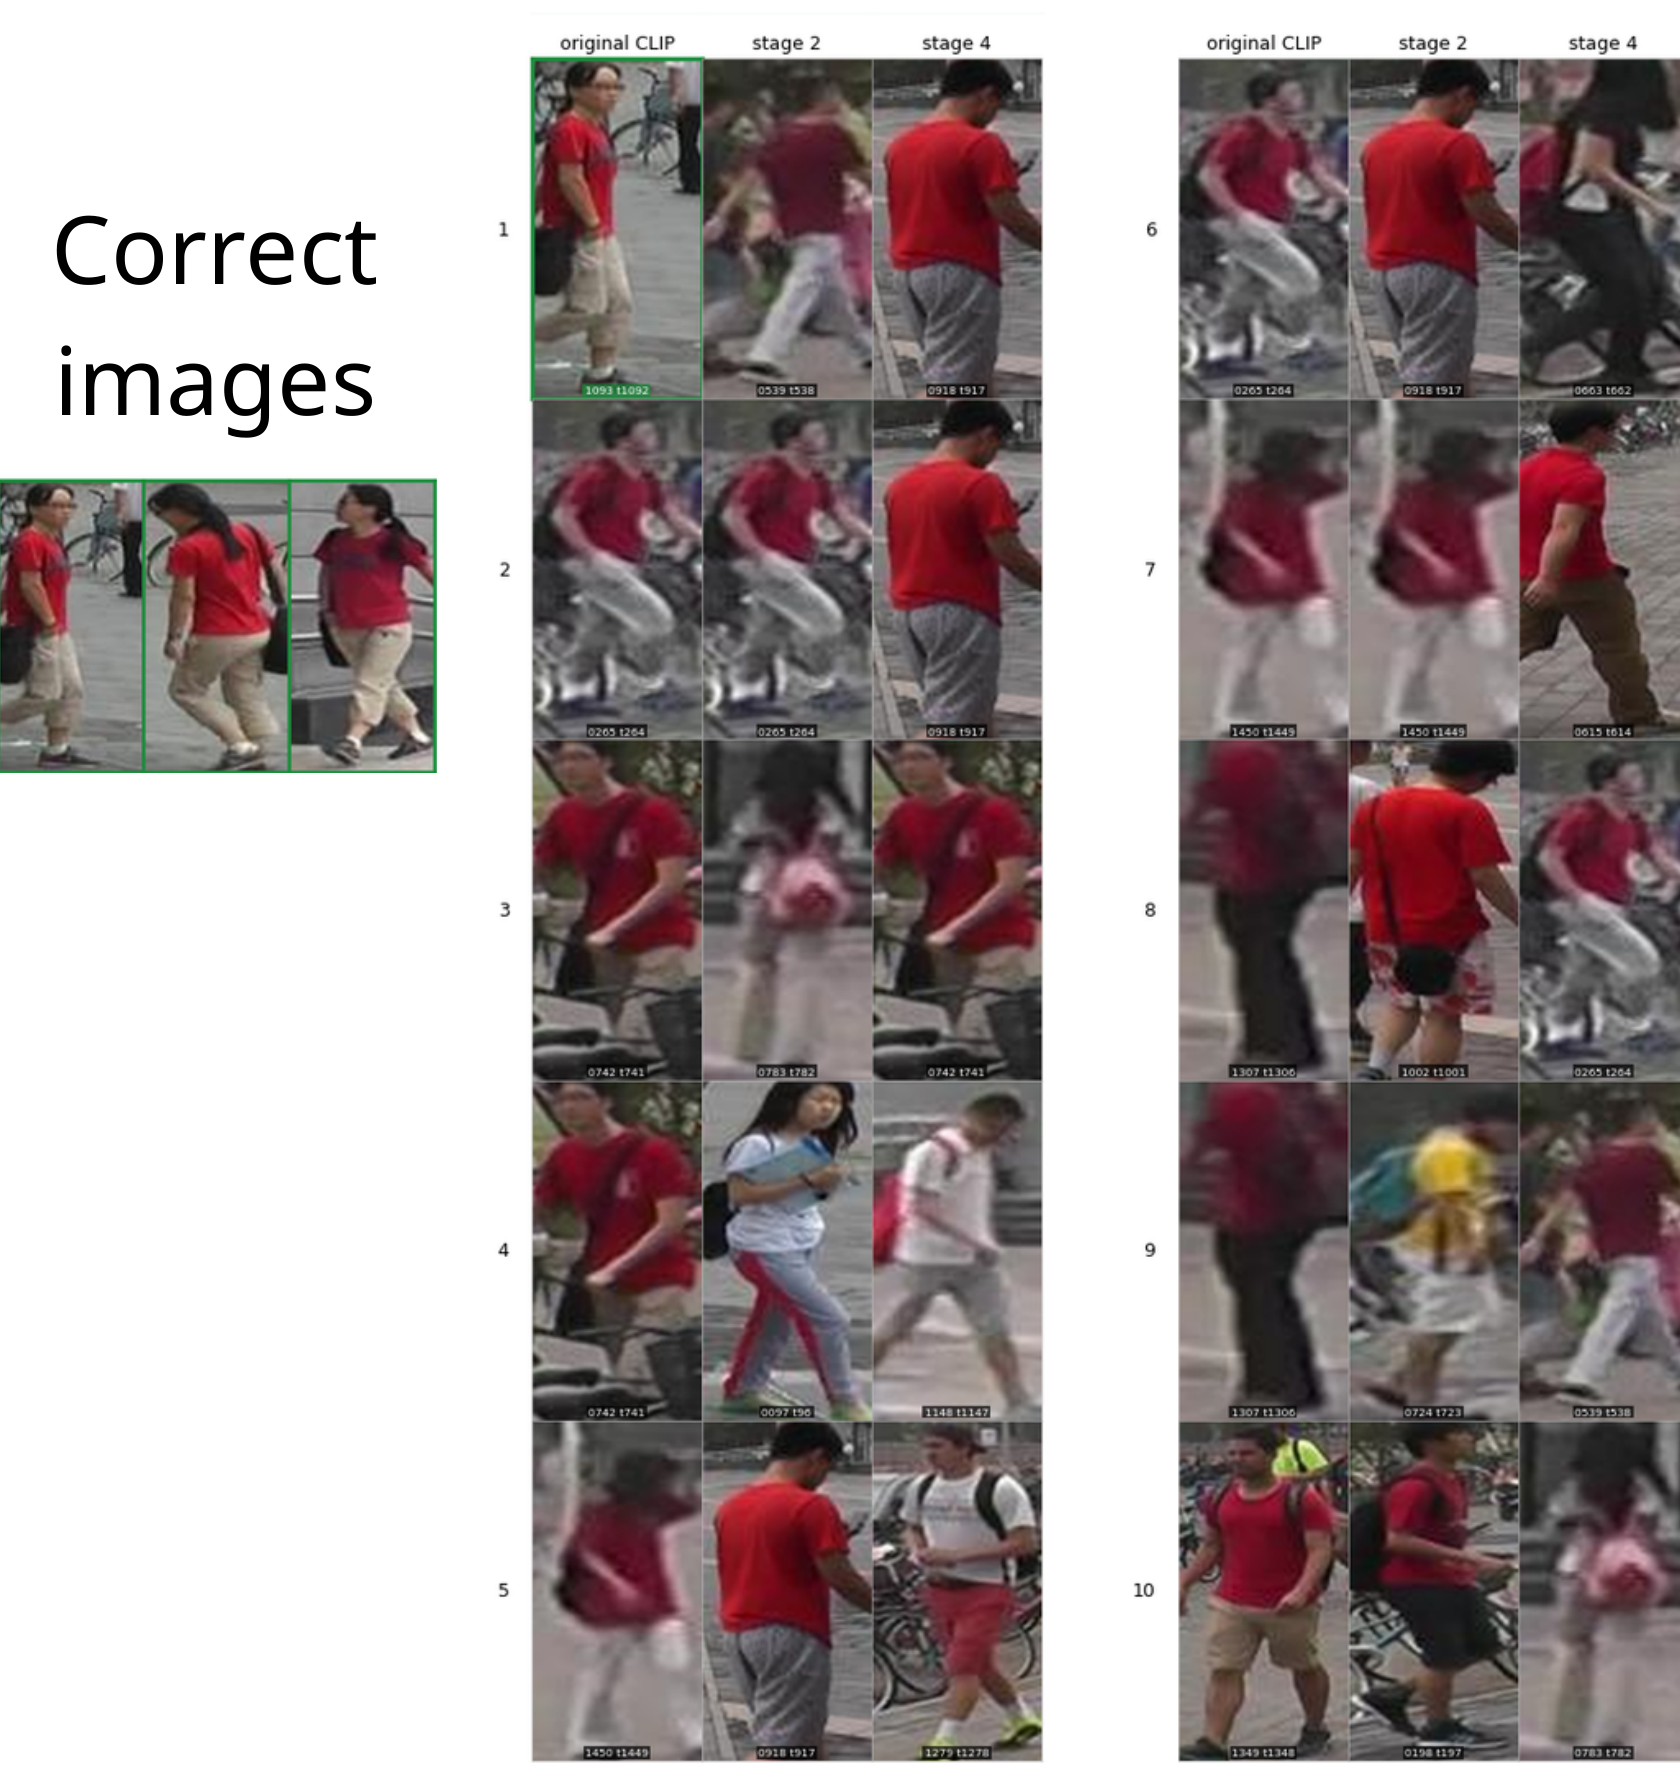
\includegraphics[width=\textwidth,height=0.78\textheight,keepaspectratio]{case_lost.png}
\caption{A lost case. Left: three gallery crops of the correct person. Right:
the CLIP ordering and the two funnel rounds, ranks 1 to 5 and 6 to 10.}
\label{fig:r-case-lost}
\end{figure}

\paragraph{The same case after the re-run (Figure~\ref{fig:r-case-lost-fixed}).}
The query and the evidence are identical, and only the two ranking calls are
answered by the larger model. The correct identity returns to the top of both
rounds. Nothing else in the pipeline changed, which makes the comparison direct.

\begin{figure}[H]
\centering
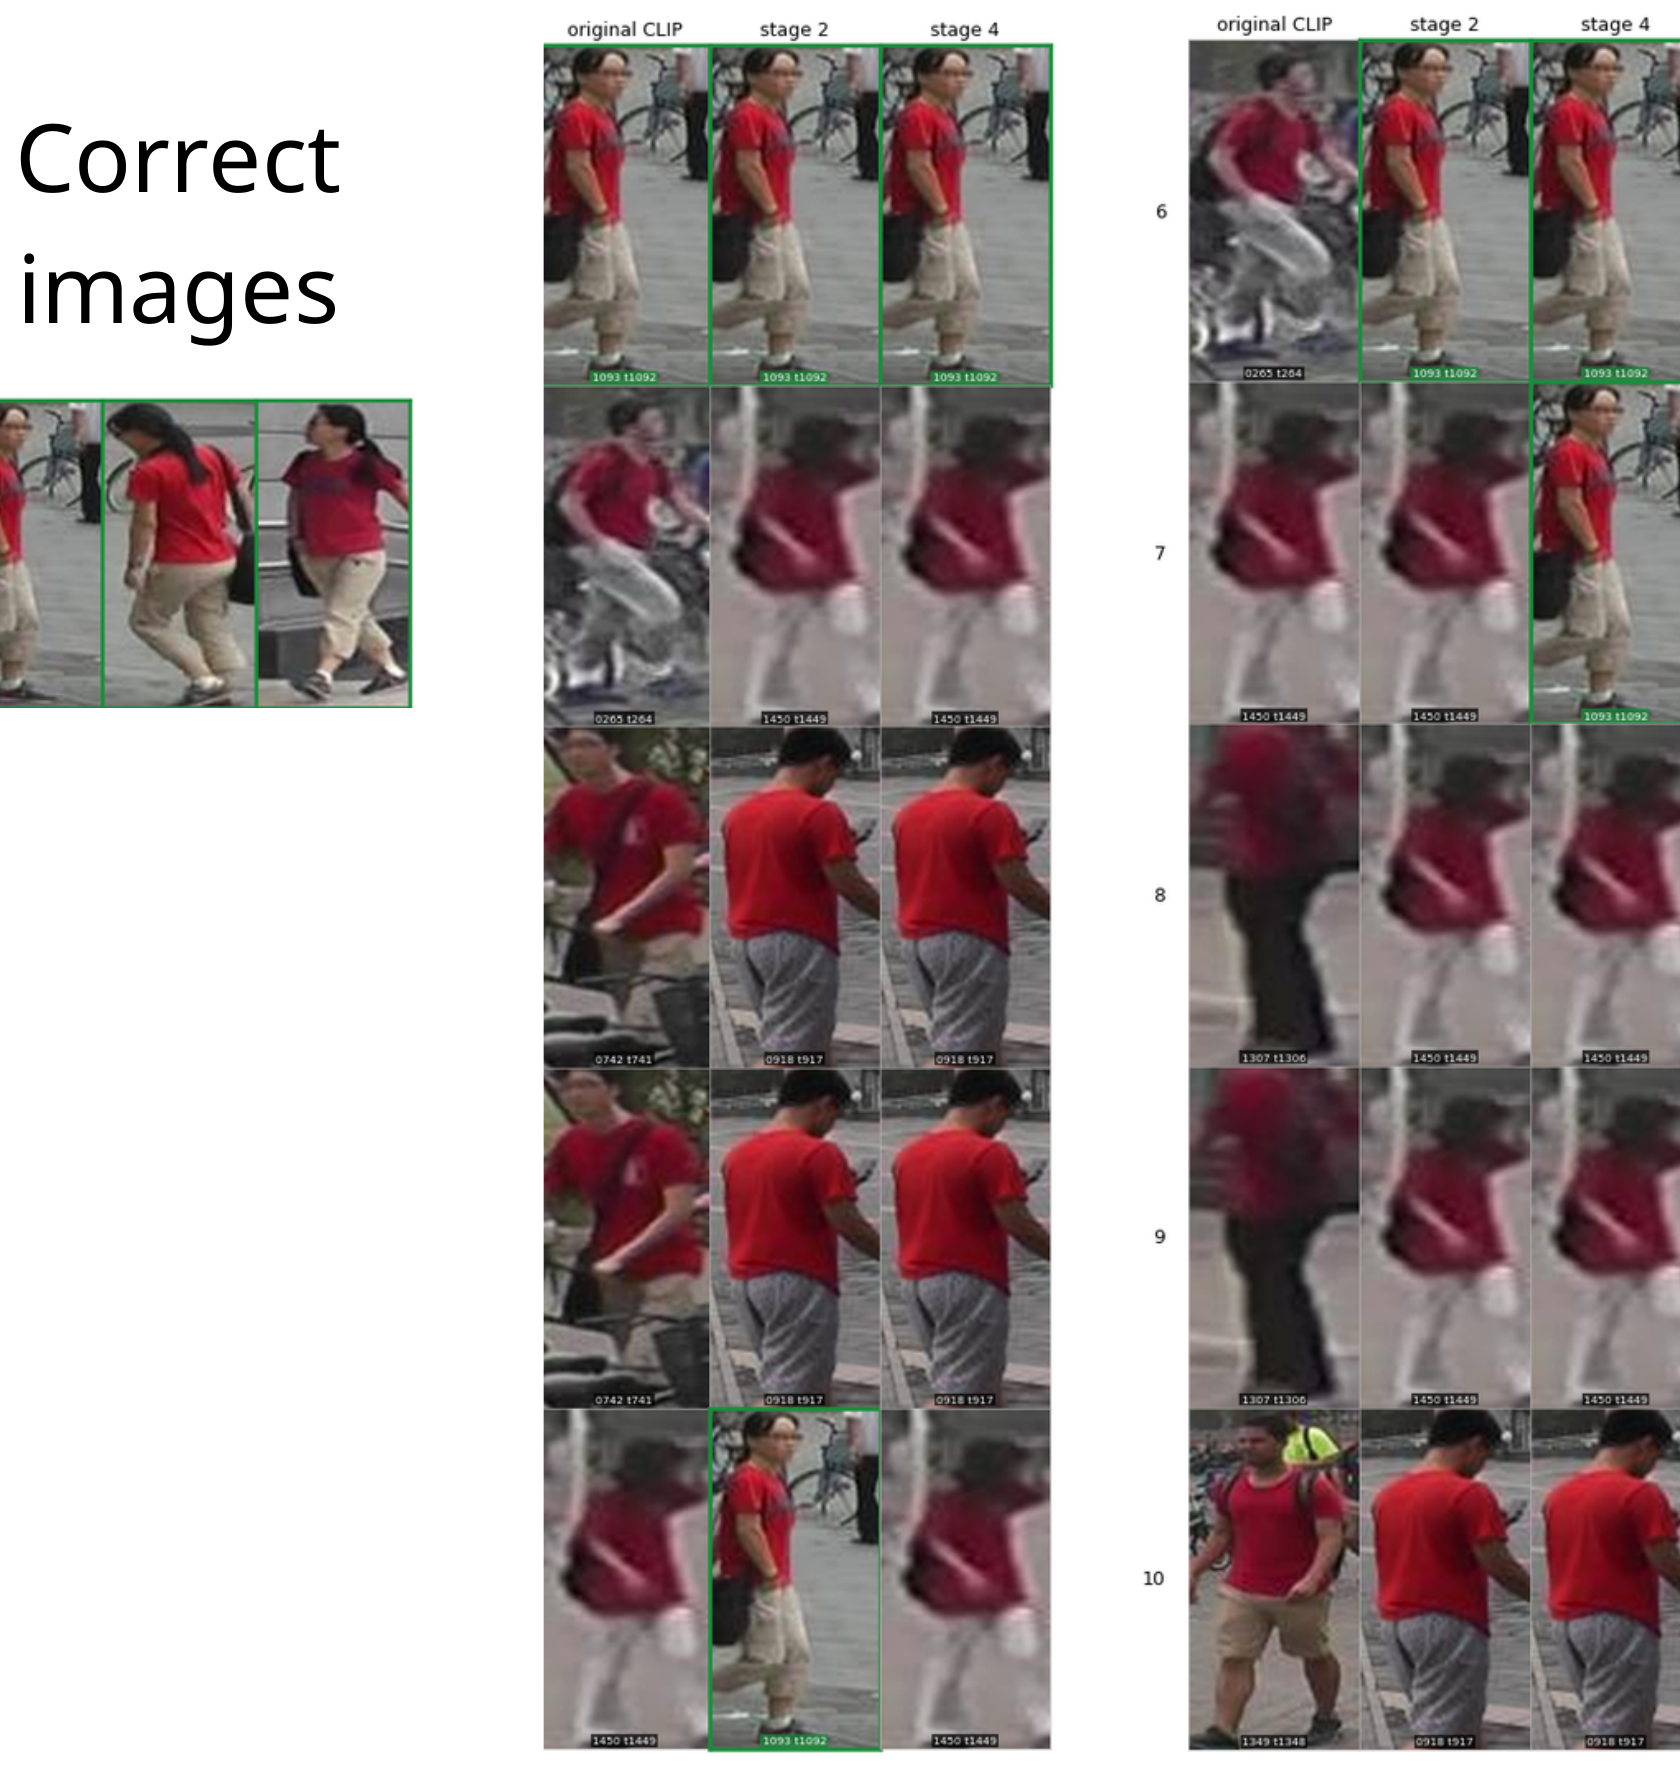
\includegraphics[width=\textwidth,height=0.78\textheight,keepaspectratio]{case_lost_fixed.png}
\caption{The same query after re-ranking with the larger model at stages 2B and
4B only. Stages 0, 1 and 2A were replayed unchanged.}
\label{fig:r-case-lost-fixed}
\end{figure}

\paragraph{A rescued case (Figure~\ref{fig:r-case-rescued}).}
Query: \emph{``A teenage man, with long hair, wearing a short-sleeve purple top
and blue trousers, with a handbag.''} CLIP's top 10 does not contain the right
person, while the funnel's does and places them first. The figure also shows
something that the recall figure cannot: the funnel gathers \emph{several crops of
the same identity} into its ten results without being told that the crops of one
track belong to one person. The grouping follows from the attribute evidence.

\begin{figure}[H]
\centering
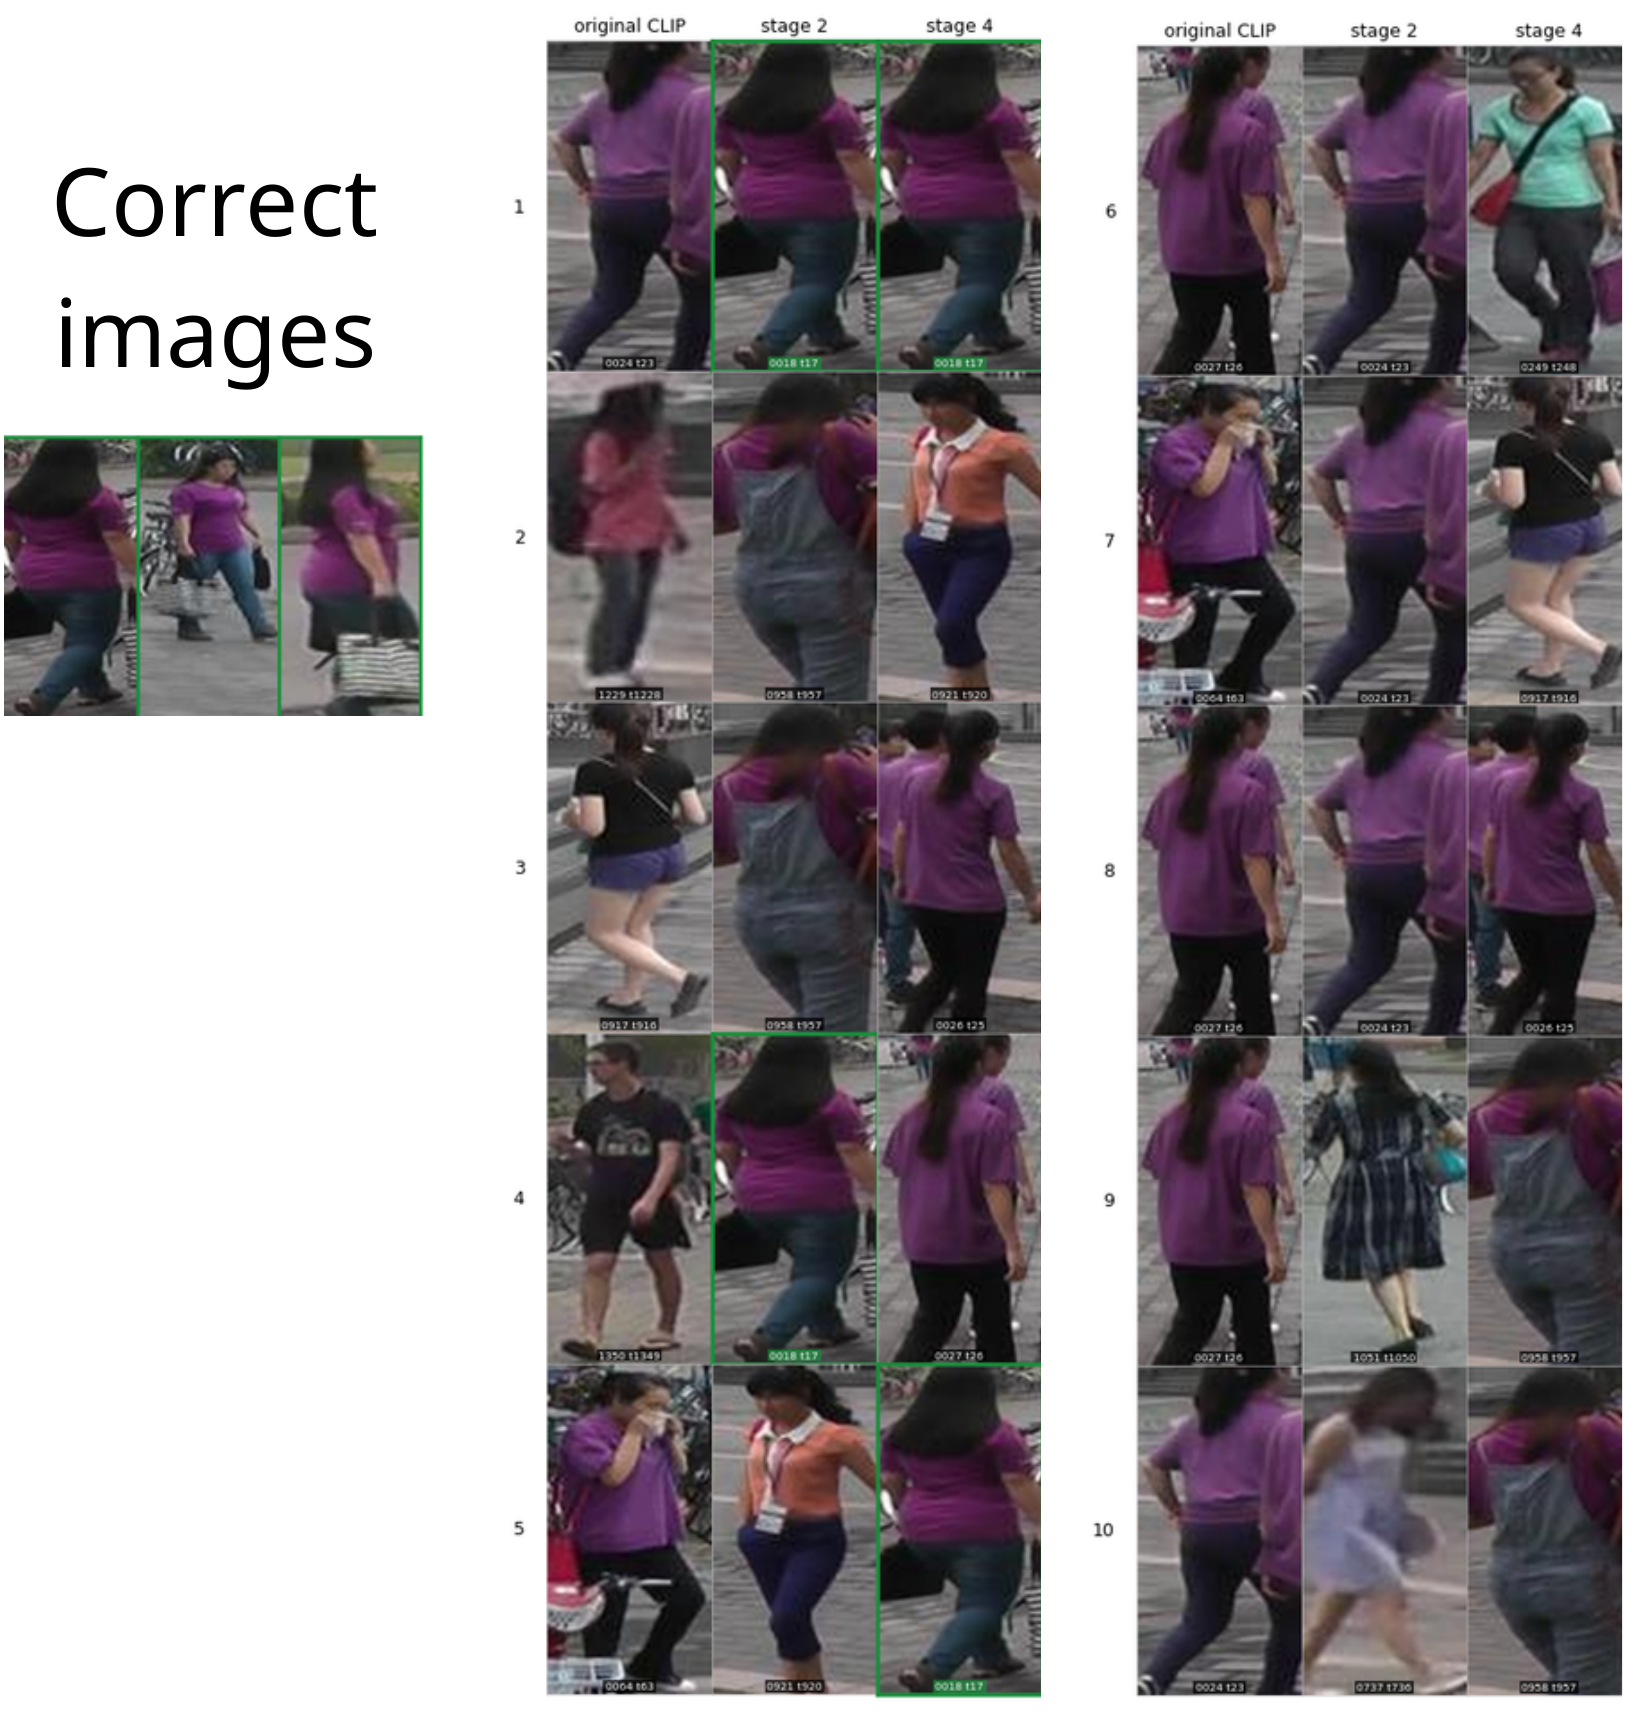
\includegraphics[width=\textwidth,height=0.78\textheight,keepaspectratio]{case_rescued.png}
\caption{A rescued case: outside CLIP's top 10, first after reasoning.}
\label{fig:r-case-rescued}
\end{figure}

\subsection{Error analysis}
\label{sec:r-error}
Combining the three tables, the sample of 100 identities divides as follows.

\begin{itemize}
\item 3 were never retrieved. The ground truth is outside the 75-crop pool, so no
      reranking could return it. This can only be fixed in retrieval, and the
      number is small.
\item 56 are returned, 28 of them only because the reasoning layer rescued them.
\item 5 were lost by the funnel after being found by CLIP.
      Section~\ref{sec:r-rerun} shows that four of these five are recovered by a
      larger model reading the \emph{same} evidence, so they are ranking failures,
      not evidence failures.
\item 36 were missed by both methods. They fall into two kinds that can be named
      but have not yet been counted separately at $n=100$: ambiguous attributes,
      where the describer itself is unsure (above all gender on small,
      rear-facing crops), and unread attributes, where a value was never written.
      Accessories are the clearest example: \at{carrying} is unread 28\% of the
      time, more often than its most common value \at{backpack} is read, so a
      query that relies on an accessory favours candidates whose accessory
      \emph{happened} to be described.
\end{itemize}

The failures of the reasoning layer itself, the five lost identities, form the
smallest category and the easiest to address; the large remainder comes from
upstream, from what the index contains.

% =========================================================== 8 ablations ====
\section{Ablations and Design Decisions}
\label{sec:r-ablation}

Almost every mechanism in Section~\ref{sec:r-reasoning} was added in response to a
measured failure rather than planned in advance, and most of them can still be
switched off. This section states, for each mechanism, what it changed and how
strong the evidence is, separating what was \emph{measured} from what is only
\emph{switchable}.

Two limitations apply to all of these numbers.

\paragraph{The sample behind a prompt measurement is a batch, not a sweep.} The
prompt-level numbers below were collected while developing each stage, on batches
of 25 to 75 candidates. They are large, categorical differences (19 to 0, 0 of 82)
rather than narrow ones, which is why they are reported, but they are not recall
measurements over 100 identities.

\paragraph{The model fixes a style per call.} Two batches with the same prompt,
run one after the other, produced 0 of 73 and 73 of 73 notes carrying a boundary
citation. The convention a call adopts at its first contested note holds for the
rest of that call. Any A/B comparison of prompt wording must therefore be read
across several calls, since a single-call comparison of two prompts may only
reflect this style lock.

% Longtable (2026-09-30): the table is taller than a page and a [H] float ran into the bottom margin.
\begin{longtable}{@{}P{4.0cm}P{5.7cm}P{5.4cm}@{}}
\caption{What each mechanism changed, and how strong the evidence is.}\label{tab:r-ablation}\\
\toprule
\textbf{Mechanism} & \textbf{What it changed} & \textbf{Evidence}\\
\midrule
\endfirsthead
\multicolumn{3}{l}{\textit{(continued from Table~\ref{tab:r-ablation})}}\\
\toprule
\textbf{Mechanism} & \textbf{What it changed} & \textbf{Evidence}\\
\midrule
\endhead
\bottomrule
\endlastfoot
Citation rule (2A): never name a mechanism without its figure
& Invented causes disappeared; every named mechanism carries a number.
& \textsc{measured}: 19 invented causes $\rightarrow$ 0; mechanism-without-figure
  0 of 82.\\
\addlinespace
Conditions channel (2A): render the per-region quality figures and pair them with
the value they explain
& The reader began citing capture conditions instead of only counts.
& \textsc{measured}: notes citing a condition with its figure 0 $\rightarrow$ 53
  $\rightarrow$ 73 of 75 across two prompt revisions.\\
\addlinespace
Reliability, not direction (2B)
& Stopped the ranker from opening every row with attributes the whole pool
  shares.
& \textsc{measured}: 69 of 75 rows had opened with the same shared-attribute
  phrase.\\
\addlinespace
Rarity table (2B/4B): state what each query value is worth in the index
& Gave the ranker a rarity channel it did not otherwise have.
& \textsc{measured} as a failure without it: 40 of 40 reasons led with the lower
  colour; gender appeared in 2, while gender split the pool 44/31.\\
\addlinespace
Coverage floor, round-dependent
& Protects a present-but-weak reading from the \emph{unrecoverable} coarse cut
  only.
& \textsc{reasoned}: the coarse cut cannot be undone and the refine cut can.
  Not A/B tested.\\
\addlinespace
Dropping \code{stab} from the decisive gate
& The floor applies to rare values even when the describer writes them
  unsteadily.
& \textsc{measured}: on one query every rare value scored $\text{stab}<0.20$,
  nothing was called decisive, and the floor never applied.\\
\addlinespace
Stage 1/3 restricted to query-constrained attributes
& Stopped the selector from spending slots on attributes the query never
  mentioned.
& \textsc{reasoned} from the selections; not A/B tested.\\
\addlinespace
CLIP score withheld from 2B/4B
& The ranker orders on evidence alone.
& \textsc{measured}: AUC 0.601 within the pool, adjacent-rank gap 2.7\% of one
  sd (Table~\ref{tab:r-clipscore}).\\
\addlinespace
The refine round (4 stages vs 2)
& $+3$ identities at R@10, $-8$ at R@1 and $-8$ at R@5.
& \textsc{measured}, $n=100$ (Table~\ref{tab:r-main}); both records come from the
  same run, so the comparison is paired.\\
\addlinespace
Model at the ranking stages
& 4 of 5 ranking failures recovered on identical evidence.
& \textsc{measured} on 5 oracle-selected queries (Table~\ref{tab:r-rerun}).\\
\end{longtable}

\paragraph{Switchable but not yet measured.} The pipeline has one flag per
experiment so that these comparisons can be run: \code{LAB\_QUALITY\_POPULATION}
(region quartiles over the candidate crops rather than over every frame of their
tracks), \code{LAB\_PAIR\_PROFILE} (the per-pair statistics block),
\code{LAB\_FRAME\_AGREEMENT} (the \code{agrees} line under each quoted frame),
\code{LAB\_TYPICAL\_GUARD}, and \code{VIEW\_MIN\_UNUSUAL} (how unusual a frame must
be before a \code{view} line is printed). They are separate flags rather than one
switch on purpose: the quality-population flag \emph{corrects} an earlier error,
while the others \emph{add} signal, and a result obtained with all of them on
would not show which one caused it.

{\sloppy Three further settings are configuration rather than prompt design and are also
untested: \code{CANDIDATES\_PER\_CALL} (25, the source of the output truncation
discussed in Section~\ref{sec:r-engineering}), \code{RANK\_KEEP\_EXTRA} (how many
rows past the cut the ranker must write), and the thinking level, which is HIGH at
every stage and uses roughly 70\% of the output budget on a 2A call.\par}

\paragraph{The ablation this part could not run.} The most informative experiment,
the whole sweep on the larger model, is limited by quota rather than by design.
Section~\ref{sec:r-rerun} is the part of it that could be afforded.

% ============================================================== 9 tooling ===
\section{Evaluation Tooling and Reproducibility}

Two properties of the measurement setup are reported here because they changed
results.

\paragraph{Records are rebuilt from replies, not trusted.} The sweep writes one
JSON record per configuration and one folder per query holding every stage's
rendered input and reply. Running two notebooks against the same record file
produced a \emph{lost update}: each held the whole file in memory and wrote it
back, so the later save silently dropped the other's queries, while the file still
parsed and could still be scored. The analysis notebook therefore ignores the
record files and rebuilds every ranking from the per-query folders, mapping the
ranker's numeric labels back to crops by aligning the CLIP-similarity sequence in
the saved prompt with the retrieval cache, position by position. When an alignment
check fails, the query is \emph{skipped and named}, never guessed, because
attaching a reply's labels to the wrong candidate list would produce a complete,
plausible and wrong record.

\paragraph{Every rate is reported with its denominator and its ceiling.} Queries
with no ground-truth track are counted and excluded rather than silently dropped,
since a dropped query inflates every rate by shrinking the denominator.
\code{cap@75} is stored per query rather than as one rate, so any later subset can
recompute its own ceiling.

The supporting tools built for this analysis are: a per-identity viewer showing
the ground truth's CLIP rank and its rank after each stage together with the
ranker's reason; a \emph{funnel-lost} report listing the identities that CLIP had
in its top 10 and the funnel did not (the source of Tables~\ref{tab:r-lost}
and~\ref{tab:r-lostwhy}); a coverage table over all evaluated identities; and a
work-queue notebook that classifies every full-pool query not yet evaluated as
\emph{CLIP hit}, \emph{miss but inside the pool} (what reranking can still gain)
or \emph{miss outside the pool} (to be fixed in retrieval).

% ============================================================ 9 limitations =


% ---- Shared
% Chapter 12 is shared by both parts: a gap in the TOC and a root-level bookmark keep it out of Part II.
\addtocontents{toc}{\protect\addvspace{1.5em}}
\bookmarksetup{startatroot}
% !TEX root = ../../main.tex
% Chapter 12 (shared) - the Vietnamese Chapter 9 translated, with the Part II results, limitations and future work
% taken from the research report (sections/research/_conclusion.tex, _limits.tex). Each section is split by part.
\chapter{Conclusion and Future Work}
\label{chapter:tongket}

\textit{This chapter summarises the results of both parts of the project, the limitations that remain and the directions for future work.}

% !TEX root = ../../main.tex
% C12.1 - Achievements. 12.1.1 = Vietnamese 9.1 translated (Part I); 12.1.2 = research conclusion (Part II), verbatim.
\section{Achievements}
\label{sec:9.1}

\subsection{Part I: The Application}
\label{sec:12.1.1}

Against the first five objectives set in Section~\ref{sec:1.2}, the application achieved the following:
\begin{enumerate}
    \item The system turns camera data into searchable data. RTSP streams and video files go through the same pipeline of sampling, detection, tracking, representative frame selection and encoding, with a consistent write mechanism across the three data stores. The demonstration data of 1,488 tracks from the seven WILDTRACK cameras was indexed without errors (Section~\ref{sec:7.2}).
    \item All three forms of query, by image, English description and attributes, are implemented in one vector space. Search by image performs well (Recall@8 of 0.89 on 26 queries). Search by text and by attributes by the vectors alone is nearly ineffective on the test data; with RaSa's matching head re-ranking the first 128 candidates, an optional stage added after the evaluation, text search reaches Recall@8 of 0.423 and attribute search 0.154, at about 17 seconds per query on the CPU (Section~\ref{sec:8.4}).
    \item Users can view each result in its full frame and save results into case files with a status and an information snapshot. Viewers can follow these case files in read-only mode.
    \item The three roles are controlled by the permission matrix of Section~\ref{sec:4.6}, with the search scope limited by area, and the access rule of every API is tested (Section~\ref{sec:8.1}). The Administrator has tools to monitor the status, check the AI and consult the audit log.
    \item The project measured the search quality, processing speed and storage when integrating YOLO11n, ByteTrack and RaSa on a CPU-only machine (Chapter~\ref{chapter:kiemthu}). The results clearly show the strength of search by image and the limitation of search by text caused by the domain gap.
\end{enumerate}
The application runs the whole workflow from receiving camera data, searching and assessing to saving case files. The demonstration script ran automatically twice in a row with 15/15 steps passed, and the test suite of 713 unit tests together with the integration and end-to-end tests all passed.

\subsection{Part II: The Reasoning Layer}
\label{sec:12.1.2}

For the sixth objective, the research of Part~II reached the following result.

% !TEX root = ../../main.tex
% Part II (Nguyen Huu Cuong) - merged from the research report (report_latex_v3), see MERGE_NOTES.md.
% Style pass 2026-09-30: em dashes and rhetorical sentences removed; technical content, numbers and references unchanged.
% Tightened 2026-10-05 (both authors agreed).
% Used by Chapter 12, section 12.1 (Part II results).
Attribute-level evidence, rendered as text and reasoned over by a small LLM,
recovers 28 of the 67 identities that CLIP alone ranks outside its top 10, a gain
of 23 points in R@10, with no fine-tuning and on a pool produced by CLIP itself.
The gain comes not from a better similarity measure but from readable evidence:
what this crop and the rest of the track read, how strongly those frames link, and
under what imaging conditions. The CLIP score, which the ranker does not use,
separates the ground truth within its pool at an AUC of only 0.601: CLIP retrieves
well but ranks its pool poorly.

The cost is small: five of the 33 identities already found by retrieval are pushed
out, and four of them are recovered when only the two ranking calls use a larger
model over the same evidence. Most of what remains is not a ranking problem: three
of 100 identities were never retrieved, and the rest comes from attributes the
describer could not read or did not write. Both causes are measurable, and with the
ceiling reported next to every number, further work starts from a clearer position
than the project did.


% !TEX root = ../../main.tex
% C12.2 - Limitations. 12.2.1 = Vietnamese 9.2 translated (Part I); 12.2.2 = research limitations (Part II), verbatim.
\section{Limitations}
\label{sec:9.2}

\subsection{Part I: The Application}
\label{sec:12.2.1}

The experiments confirm the limitations stated in Section~\ref{sec:1.4}. The largest is that search by text and by attributes is not yet effective on the test data: no query has a correct result in the top 16 (Section~\ref{sec:8.4}). The cause is the domain gap between RaSa's training data and person images cropped automatically from cameras.

On a CPU-only machine, processing is about seven times slower than real time. The system has to process the cameras in turn, part of the frames of a live stream are skipped, and the demonstration data had to be indexed from video files (Section~\ref{sec:7.2}). RTSP data is also only encoded and written at the end of each session, rather than as soon as each appearance ends, so there is a delay between a person appearing in front of a camera and becoming searchable (Section~\ref{sec:5.2.1}). RTSP frames are also timestamped when read rather than by the stream, so slow processing widens the gap between processed frames, ending tracks early and splitting appearances (Section~\ref{sec:3.3.5}); video files are not affected. The first search needs a warm-up to load the encoder, and memory is tight: with the server and the pipeline each loading their own models, processing uses about 8~GiB, nearly exhausting a 16~GB machine with other applications open (Section~\ref{sec:8.7}).

Finally, the evaluation is incomplete: the quality of search by image and by text at the current confidence threshold has not been measured again (Section~\ref{sec:8.4}). BoT-SORT is integrated but has not been used for indexing or evaluated.

\subsection{Part II: The Reasoning Layer}
\label{sec:12.2.2}

% !TEX root = ../../main.tex
% Part II (Nguyen Huu Cuong) - merged from the research report (report_latex_v3), see MERGE_NOTES.md.
% Style pass 2026-09-30: em dashes and rhetorical sentences removed; technical content, numbers and references unchanged.
% Used by Chapter 12, section 12.2 (Part II limitations).
\label{sec:r-limits}
\paragraph{Model.} The reasoning LLM is Flash-Lite 3.5, chosen for its larger
free-tier allowance rather than its quality. Section~\ref{sec:r-rerun} confirms
that this is a limitation: it recovers four of five ranking failures by switching
the two ranking calls to a larger model and changing nothing else. A full sweep on
the larger model is the most direct improvement available and has not been run;
the re-run covers five oracle-selected queries, not the sample.

\paragraph{Data.} Token limits restricted the evaluation to 100 of the 496
uniquely identifiable identities, so practical usability is not yet established,
and the subset itself is an easier population than the full 1501 identities
(Section~\ref{sec:r-dataset}). At $n=100$ a percentage point is one identity, and
the R@1 ordering in Table~\ref{tab:r-main} rests on differences of 3 and 8
identities. Extending the sweep requires no new work: the work-queue notebook
already selects the next identities to run, giving priority to queries whose
ground truth is inside the pool but outside CLIP's top 10.

\paragraph{The blocks this part did not change.} Detection and tracking were filled
with established defaults and left unchanged (Section~\ref{sec:r-choices}), and
their failures still reach the search block: a person the detector missed has no
crop, and a track merged by the tracker contains two people under one identity.
This part measures neither. A tracker-error analysis over the same 100 identities
is the next measurement to make, and it would move part of what
Section~\ref{sec:r-error} counts as a reasoning residue into an upstream category.

\paragraph{The refine round.} Four stages beat two at R@10 and lose to two at R@1
and R@5, and three of the five losses in Table~\ref{tab:r-lostwhy} were caused by
the refine round. Whether stages 3 and 4 should return a full ranking, or only
re-order the candidates the coarse round was unsure about, is still open.

\paragraph{Rarity versus mismatch cost.} The rarity table tells the ranker what a
query value is worth when it separates candidates. It does not yet state the
converse: a \emph{binary} attribute such as gender is ``almost nothing'' by rarity
(both values are common), yet a gender mismatch is the strongest exclusion
available. On one measured query, 40 of 40 reasons led with the lower colour and
gender appeared in 2, while gender split the pool 44 to 31. This asymmetry between
rarity and mismatch cost remains to be handled.

\paragraph{Output truncation.} At 25 candidates per 2A call, replies occasionally
stop at the output limit in the middle of a unit. The limit is currently detected
after the fact from the API's finish reason rather than requested explicitly, and
the two direct fixes, sending an explicit output cap or reducing the batch to 15
candidates, have not yet been compared.

\paragraph{Single phrasing.} Each identity is queried with one descriptive
sentence. Robustness to paraphrase is not measured, although the pipeline already
supports several phrasings per identity.


% !TEX root = ../../main.tex
% C12.3 - Future work. 12.3.1 = Vietnamese 9.3 translated (Part I); 12.3.2 = [MERGE] link between the two parts (to be reviewed).
\section{Future Work}
\label{sec:9.3}

\subsection{Part I: The Application}
\label{sec:12.3.1}

The priority is to improve search by text and by attributes. RaSa's re-ranking with its multimodal encoder is now an optional stage of the search flow and is where the model's accuracy lies (Section~\ref{sec:8.4}); making it fast enough for everyday use means computing the image tokens of each appearance at indexing time, in the background worker, instead of at the first search, and running the fusion passes on a GPU, where 128 candidates take well under a second. The measurement of Section~\ref{sec:8.4} also points to a simpler route: a second vector per appearance from a CLIP-like encoder, computed at indexing time and stored in its own Milvus collection, would give text and attribute search close to the re-ranked quality at the cost of one more vector search, while RaSa's vectors keep serving image queries; the design already keeps one collection per encoder version, so the change is contained in the indexing pipeline and the query router. Fine-tuning either model on data from the same domain as surveillance cameras remains the step after that.

For memory, one encoder process shared by the application server and the background worker would remove one of the two copies of the query encoder, about 1~GiB. For speed, inference on the CPU could be optimised, for example with OpenVINO, starting with the image encoder, which takes most of the processing time (Section~\ref{sec:8.5}), or the system could be deployed on a machine with a GPU to analyse many camera streams at the same time instead of in turn. Once the system keeps up with real time, each camera could be processed continuously, and each appearance could be encoded and written as soon as it ends to shorten the delay before it becomes searchable. The write to the three stores already handles each appearance separately, so the change lies mainly in the analysis pipeline.

The evaluation should also compare ByteTrack with BoT-SORT. Further ahead, the system could link the appearances of the same person across cameras, represent each appearance with several frames, and support queries in Vietnamese.

% [MERGE] New paragraph linking the two parts - to be reviewed by both authors.
\subsection{Bringing the Two Parts Together}
\label{sec:12.3.2}

The research of Part~II addresses exactly the weakest point of the application, search by text (Section~\ref{sec:8.4}). Its reasoning layer works on a candidate pool produced by vector retrieval, which is the output the application already obtains from Milvus, so it could be placed behind the application's search step as an optional re-ranking stage. Doing so would require an attribute index built alongside the vectors during indexing, a decision on where the language model runs given the application's on-premises deployment, and a measurement of the added latency per query. The further directions of the reasoning layer itself are stated in Section~\ref{sec:12.2.2}.



\printbibliography[heading=bibintoc,title={References}]

% Appendix A (verbatim prompts, ~54 pages) removed 2026-10-04 on the supervisor's advice: nobody reads it in print;
% the prompts stay in prompts/ beside the source. Restore with the two lines below.
% \appendix
% % !TEX root = ../../main.tex
% Part II (Nguyen Huu Cuong) - merged from the research report (report_latex_v3), see MERGE_NOTES.md.
\chapter{System Prompts of Part II}
\label{app:prompts}

The prompts are reproduced verbatim, as sent to the model. Every design decision
discussed in Section~\ref{sec:r-reasoning} and listed in Table~\ref{tab:r-ablation}
appears here as text. Placeholders in braces are filled by the renderers described
in Section~\ref{sec:r-reasoning}; the user messages show what data each stage
receives.

The two ranking rounds share one system prompt and differ only in the coverage
block inserted into it: \code{COVERAGE\_COARSE} for the $75\rightarrow25$ cut and
\code{COVERAGE\_FINAL} for the $25\rightarrow10$ cut. Stage 3 uses the prompt of
stage 1 with one paragraph inserted.

\section{Stage 0: query analyst}
\VerbatimInput[fontsize=\footnotesize,breaklines=true,breakanywhere=true,
               frame=leftline,framesep=4mm]{prompts/STAGE0_SYS.txt}
\paragraph{User message.}
\VerbatimInput[fontsize=\footnotesize,breaklines=true,breakanywhere=true,
               frame=leftline,framesep=4mm]{prompts/STAGE0_USER.txt}

\section{Stage 1: attribute-value selector}
\VerbatimInput[fontsize=\footnotesize,breaklines=true,breakanywhere=true,
               frame=leftline,framesep=4mm]{prompts/STAGE1_SYS.txt}
\paragraph{User message.}
\VerbatimInput[fontsize=\footnotesize,breaklines=true,breakanywhere=true,
               frame=leftline,framesep=4mm]{prompts/STAGE1_USER.txt}

\section{Stage 3: the refine selector's insertion}
Stage 3 sends the stage 1 prompt above with this paragraph added, and the anchor
phrase \emph{``VALUE for distinguishing candidates.''} replaced by it.
\VerbatimInput[fontsize=\footnotesize,breaklines=true,breakanywhere=true,
               frame=leftline,framesep=4mm]{prompts/STAGE3_REFINE.txt}

\section{Stage 2A / 4A: evidence reader}
\VerbatimInput[fontsize=\footnotesize,breaklines=true,breakanywhere=true,
               frame=leftline,framesep=4mm]{prompts/STAGE2A_SYS.txt}
\paragraph{User message.}
\VerbatimInput[fontsize=\footnotesize,breaklines=true,breakanywhere=true,
               frame=leftline,framesep=4mm]{prompts/STAGE2A_USER.txt}

\section{Stage 2B / 4B: the ranker}
\VerbatimInput[fontsize=\footnotesize,breaklines=true,breakanywhere=true,
               frame=leftline,framesep=4mm]{prompts/STAGE2B_SYS.txt}
\paragraph{User message.}
\VerbatimInput[fontsize=\footnotesize,breaklines=true,breakanywhere=true,
               frame=leftline,framesep=4mm]{prompts/STAGE2B_USER.txt}

\section{The coverage blocks}
\code{\{COVERAGE\}} in the ranker's system prompt is one of these two.
\paragraph{Coarse round ($75\rightarrow25$).}
\VerbatimInput[fontsize=\footnotesize,breaklines=true,breakanywhere=true,
               frame=leftline,framesep=4mm]{prompts/COVERAGE_COARSE.txt}
\paragraph{Final round ($25\rightarrow10$).}
\VerbatimInput[fontsize=\footnotesize,breaklines=true,breakanywhere=true,
               frame=leftline,framesep=4mm]{prompts/COVERAGE_FINAL.txt}

% ============================================================ references ====


\end{document}
